\RequirePackage{amsthm} % theorems, definitions etc.; needs to be loaded before "newtxmath", which is loaded by SDQ class

\documentclass[format=a4-sdq]{sdqdiss} % format used in dissertations of our chair
% SDQ class and template from https://gitlab.kit.edu/kit/kastel/sdq/dokumentvorlagen/sdq-dissertations-vorlage (commit e8956c532bc75db4c245cb3304325436bfc4d281 "Anpassung Titelseite auf Prüfungsordnung" (Jun 12, 2023))

%%% Packages %%%

\PassOptionsToPackage{hyphens}{url} % "url" is loaded by "hyperref", but we need to set an option for it (allow line breaks after "-" character)

\usepackage[linesnumbered,ruled,vlined]{algorithm2e} % pseudo-code
%\usepackage{amsmath} % mathematical symbols and equations; loaded by "newtxmath", which is loaded by SDQ class
%\usepackage{amssymb} % mathematical symbols; alternatively provided by "newtxmath", which is loaded by SDQ class
%\usepackage{amsthm} % theorems, definitions etc.; loaded before SDQ class
\usepackage[ngerman,english]{babel} % switching languages
\usepackage[citestyle=numeric,style=numeric,backend=biber]{biblatex}
\usepackage{booktabs} % nicely formatted tables (with top, mid, and bottom rule)
\usepackage{csquotes} % expected by "babel", which is used for language switching
%\usepackage{enumitem} % nicely formatted enumerations; loaded by SDQ class
%\usepackage[T1]{fontenc} % was loaded in SDQ template
%\usepackage{graphicx} % plots; loaded by "wallpaper", which is loaded by SDQ class
\usepackage{multirow} % cells spanning multiple rows in tables
\usepackage{pdfpages} % for the licensing disclaimer on the back of the title page
\usepackage{subcaption} % figures with multiple sub-figures and sub-captions
%\usepackage{url} % \url command; loaded by "hyperref"
%\usepackage{hyperref} % links and URLs; loaded by "pdfx"
\usepackage[a-1a]{pdfx} % create a PDF/A document (still not fully compliant, but more than before)

%%% Meta-data %%%

% see also "dissertation.xmpdata" for meta-data attached to the PDF file
\title{Leveraging Constraints for User-Centric Feature Selection}
\author{Jakob Bach}
\date{} % printed below author, is disabled if empty (but not if commented out); unused in dissertations of our chair
%\subject{} % printed above title; unused in dissertations of our chair

%%% Setup %%%

\pdfsuppresswarningpagegroup=1 % hide warning for multiple PDFs (e.g., figures) being on one page

\addbibresource{references.bib}

\setlength{\algomargin}{1em} % prevents pseudo-code algorithms' line numbers from appearing on margins of page

\renewcommand{\floatpagefraction}{0.5} % reset minimum fraction of a float-only page that must be occupied by floats to the LaTeX default; SDQ class uses a higher threshold, which causes some of our float-only pages (using [p] as position) to be moved to end of chapter since they are not filled up to this threshold

\newcommand{\Abstract}[1][Abstract]{\chapter*{#1}\addcontentsline{toc}{chapter}{#1}\markboth{#1}{#1}} % from SDQ template; just a special kind of chapter

\newtheorem{definition}{Definition}
\newtheorem{example}{Example}
\newtheorem{proposition}{Proposition}

%%% Title page %%%

\subtitle{
	\vskip2em
	Zur Erlangung des akademischen Grades eines\\[1em]
	{\Large Doktors der Ingenieurwissenschaften}\\[1em]
	von der KIT-Fakultät für Informatik des\\
	Karlsruher Instituts für Technologie (KIT)\\[.5em]
	genehmigte\\[.3em]
	{\Large Dissertation}
}

\author{
	\normalsize{von}\\
	{\LARGE Jakob Bach}\\
}

\publishers{%
	\flushleft\small
	Tag der mündlichen Prüfung: 20. Januar 2025\\
	1. Referent/Referentin: T.T.-Prof. Dr. Peer Nowack\\
	2. Referent/Referentin: Prof. Dr. Ira Assent\\
}

\begin{document}

%%% Front matter %%%

\pagenumbering{alph} % supresses "destination with the same identifier" warnings that are caused by title page being numered arabic by default (though not visible), same as main matter (which causes clash for "hyperref")
\selectlanguage{ngerman}
\maketitle

% license page downloaded from https://www.bibliothek.kit.edu/downloads/PDF/CC_Lizenzvermerke.zip
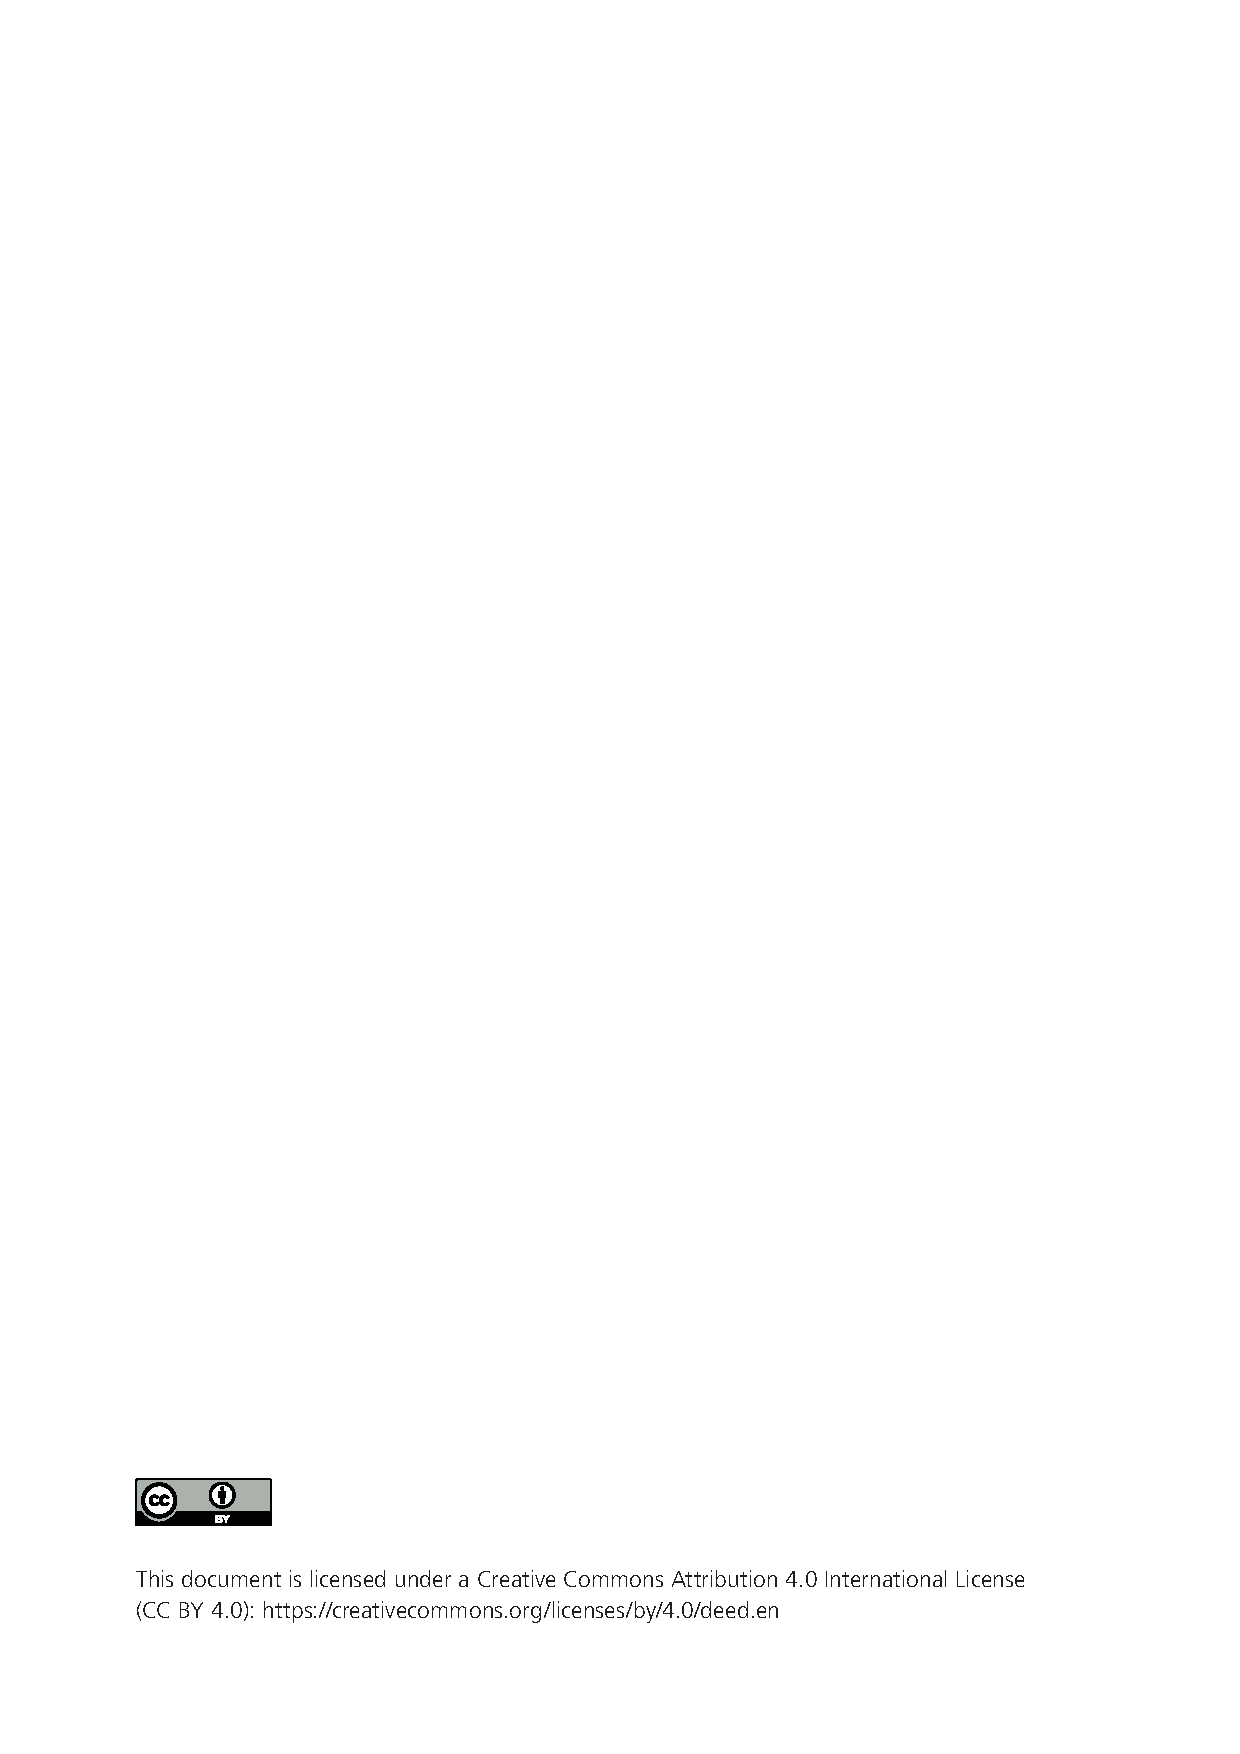
\includepdf{CC-BY_Vermerk_A4_2017_4.0_EN.pdf}

\frontmatter % uses roman page numbers

\selectlanguage{english}
\Abstract[Acknowledgments]{Obtaining a PhD is a long and challenging process, with many ups, downs, and intermediate results on the way there.
Nevertheless, all that formally matters are the dissertation and defense at the very end.
In this sense, I want to thank Prof. Peer Nowack and Prof. Ira Assent for serving as reviewers, Prof. Benjamin Schäfer for serving as the third examiner, and Prof. Klemens Böhm for the freedom and funding in the many years before.

To all PhD students reading this text:
Do not be fooled by the large number of people who are often mentioned in a dissertation's acknowledgments.
The PhD is, first and foremost, a personal project and essentially depends on your own motivation and work.
It can be a very lonely struggle from time to time.
If you do not advance your PhD project, nobody else will do.
However, other researchers and non-researchers can (and should) have a positive impact on your PhD's success, generally and in my personal case.

In the context of this dissertation, I want to thank Holger Trittenbach and Vadim Arzamasov for inspiration and advice on the topics that constitute my PhD research.
Further, my gratitude goes to Florian, Miki, Stas, and Tobias for proofreading.
Additional thanks go to all attendees of my defense and to those who made me a nice hat.

In the context of my work at KIT, several other persons made my PhD years more pleasant.
Elaheh, Markus, Pawel, and Tobias: Thanks for the successful collaborations and for showing me that collaborative research is much more fun than working alone, subject to having the right collaborators.
Edouard: Thanks for our joint undertaking to enhance the data science course.
Federico: Thanks for the sound teamwork regarding, but not limited to, the data science lab course.
Miki: Thanks for bringing cakes, games, and humor to the chair.
Pawel: Thanks for deep conversations on the PhD, research in general, and various other topics.
The rest of the chair: Thanks for also being there (participation trophy).
I particularly want to thank my fellow board-game and table-soccer players.
For legal reasons, I hereby declare that all playing took place during breaks and after work.

Finally, I want to thank my family and friends for their moral support, though they will not read this dissertation anyway.
(Honestly -- why should they?)
Special thanks go to my mum, whose systematic bread-slicing activities inspired me to investigate the problem of \textsc{Number Partitioning}, which kicked off my journey into complexity theory.
}
\Abstract{Feature selection in machine learning aims to identify the variables in a dataset that are most useful for predictions.
Feature-selection methods are ubiquitous for a variety of reasons:
They can increase prediction quality, reduce hardware requirements, and ease understanding of the data.
However, existing feature-selection methods do not satisfy user needs in certain scenarios:
(1)~Users may want to integrate domain knowledge into feature selection.
For example, established laws or hypotheses from the domain can make selecting certain feature combinations unintuitive for users.
In contrast, existing feature-selection methods typically ignore domain knowledge or only support particular types of it.
(2)~Multiple, differently composed feature sets may yield good predictions.
Such alternatives may provide users with different explanations for predictions.
In contrast, existing feature-selection methods typically yield just one feature set.

In this thesis, we make feature selection more user-centric by introducing constraints on the composition of feature sets.
Integrating such constraints into existing feature-selection methods is challenging since constraints may limit admissible feature sets arbitrarily, particularly when combining different constraint types.
In addition, constraints may negatively affect the feature sets' predictive quality.
Our contribution is fourfold:

(1) We analyze the impact of constraints on feature-selection results.
First, we formalize constrained feature selection as an optimization problem.
Our basic problem definition is independent of the feature-selection method.
To consider constraints, we propose employing a Satisfiability Modulo Theories (SMT) solver, which allows the use and combination of a wide range of constraint types.
Second, we evaluate the impact of constraints empirically.
We observe a trade-off between the strength of the constraints and the predictive quality of the selected features.
However, the effect is non-linear, i.e., strong constraints can still result in high feature-set quality.

(2) We use constraints to express and compare scientific hypotheses in a materials-science use case.
In particular, we collaborate with domain experts to formulate corresponding constraint types.
Our experiments demonstrate that some constraint types lead to differently composed feature sets with high quality, which motivates our following work.

(3) We use constraints to find alternative feature sets, i.e., feature sets that differ from others while simultaneously optimizing feature-set quality.
First, we formalize alternative feature selection with 0-1 integer linear constraints.
Users can control the number and dissimilarity of alternatives with one parameter each.
Second, we discuss how to integrate existing notions of feature-set quality as the objective of the optimization problem.
Third, we analyze the time complexity of this problem and show $\mathcal{NP}$-hardness, for a simple notion of feature-set quality already.
Fourth, we introduce heuristic approximations for the latter.
Fifth, we evaluate our approaches with five feature-selection methods.
We observe that our approaches can find high-quality alternative feature sets, and the two parameters allow users to exercise control over the quality.

(4) We use constraints to find sparse and alternative feature sets for subgroups.
Subgroup-discovery methods search interesting regions in a dataset that admit concise descriptions, e.g., a logical conjunction of bounds on feature values.
First, we formalize subgroup discovery as an SMT optimization problem.
Second, we formalize two user-centric constraint types:
(a) We make subgroup descriptions sparse by limiting the number of features used.
(b) We propose the problem of finding alternative subgroup descriptions, which use different features to describe a given subgroup.
Third, we prove $\mathcal{NP}$-hardness of optimization with either constraint type.
Fourth, we describe how to integrate both constraint types into existing heuristic subgroup-discovery methods.
Fifth, we evaluate solver-based and heuristic subgroup discovery empirically.
We observe that heuristic search methods are not only fast but also yield high-quality subgroups, even with the two constraint types.
}

\selectlanguage{ngerman}
\Abstract[Zusammenfassung]{Die Merkmalsauswahl (\emph{feature selection}) im maschinellen Lernen zielt darauf ab, die nützlichsten Variablen in einem Datensatz für Vorhersagen zu finden.
Methoden zur Merkmalsauswahl sind aus vielfältigen Gründen allgegenwärtig:
Sie können die Vorhersagequalität verbessern, Hardwareanforderungen verringern und das Verständnis der Daten erleichtern.
Allerdings reichen bestehende Methoden zur Merkmalsauswahl in bestimmten Szenarien nicht aus, um Nutzerbedürfnisse zu befriedigen:
(1)~Manche Nutzer möchten Domänenwissen in die Merkmalsauswahl miteinbeziehen.
Beispielsweise können etablierte Gesetzmäßigkeiten oder Hypothesen aus der Domäne die Auswahl bestimmter Merkmalskombinationen unintuitiv für Nutzer machen.
Bestehende Methoden zur Merkmalsauswahl ignorieren jedoch typischerweise Domänenwissen oder unterstützen nur bestimmte Arten davon.
(2)~Mehrere, unterschiedlich zusammengesetzte Merkmalsmengen können gute Vorhersagen liefern.
Solche Alternativen können Nutzern verschiedene Erklärungen für Vorhersagen bieten.
Bestehende Methoden zur Merkmalsauswahl geben jedoch typischerweise nur eine Merkmalsmenge zurück.

In dieser Dissertation machen wir die Merkmalsauswahl Nutzer-zentrierter, indem wir Nebenbedingungen (\emph{constraints}) für die Zusammensetzung der Merkmalsmengen einführen.
Die Integration solcher Nebenbedingungen in bestehende Methoden zur Merkmalsauswahl ist herausfordernd, da Nebenbedingungen die zulässigen Merkmalsmengen beliebig einschränken können, insbesondere beim Kombinieren verschiedener Arten von Nebenbedingungen.
Weiterhin können Nebenbedingungen die Vorhersagequalität der Merkmalsmengen negativ beeinflussen.
Unsere Arbeit leistet vier wesentliche Beiträge:

(1) Wir untersuchen den Einfluss von Nebenbedingungen auf die Ergebnisse der Merkmalsauswahl.
Als Erstes formalisieren wir Merkmalsauswahl unter Nebenbedingungen als ein Optimierungsproblem.
Unsere grundlegende Problemdefinition ist unabhängig von der Methode zur Merkmalsauswahl.
Um Nebenbedingungen zu berücksichtigen, setzen wir einen Löser für Satisfiability-Modulo-Theories-(SMT)-Probleme ein.
Dieser erlaubt die Nutzung und Kombination einer großen Bandbreite von Nebenbedingungen.
Als Zweites werten wir den Einfluss von Nebenbedingungen empirisch aus.
Wir beobachten einen Zielkonflikt zwischen der Stärke der Nebenbedingungen und der Vorhersagequalität der ausgewählten Merkmale.
Dieser Effekt ist jedoch nichtlinear; insbesondere können starke Nebenbedingungen immer noch zu einer hohen Qualität der Merkmalsmenge führen.

(2) Wir nutzen Nebenbedingungen zum Ausdrücken und Vergleichen wissenschaftlicher Hypothesen in einem materialwissenschaftlichen Anwendungsfall.
Insbesondere kooperieren wir mit Domänenexperten, um die entsprechenden Nebenbedingungen zu formulieren.
Unsere Experimente zeigen, dass manche Arten der Nebenbedingungen zu unterschiedlich zusammengesetzten Merkmalsmengen mit gleichzeitig hoher Qualität führen.
Dieses Ergebnis motiviert unsere folgende Arbeit.

(3) Wir nutzen Nebenbedingungen zum Finden alternativer Merkmalsmengen.
Letztere sind Merkmalsmengen, die sich von anderen Merkmalsmengen unterscheiden und gleichzeitig eine möglichst hohe Qualität erreichen sollen.
Als Erstes formalisieren wir alternative Merkmalsauswahl mittels ganzzahliger linearer Nebenbedingungen und binären Entscheidungsvariablen.
Nutzer können die Anzahl und die Unterschiedlichkeit der Alternativen durch jeweils einen Parameter bestimmen.
Als Zweites diskutieren wir, wie sich bestehende Konzepte für die Qualität von Merkmalsmengen als Zielfunktion des Optimierungsproblems integrieren lassen.
Als Drittes untersuchen wir die Zeitkomplexität des Optimierungsproblems und zeigen, dass es bereits mit einer einfachen Zielfunktion $\mathcal{NP}$-schwer ist.
Als Viertes stellen wir Näherungsheuristiken für diese Zielfunktion vor.
Als Fünftes werten wir unsere Ansätze mit fünf Methoden zur Merkmalsauswahl aus.
Wir beobachten, dass unsere Ansätze alternative Merkmalsmengen mit hoher Qualität finden können und dass die beiden Parameter den Nutzern Kontrolle über die Qualität geben.

(4) Wir nutzen Nebenbedingungen, um kleine und alternative Merkmalsmengen für Untergruppen (\emph{subgroups}) zu finden.
Methoden zur Untergruppenerkennung (\emph{subgroup discovery}) suchen in einem Datensatz nach interessanten Bereichen, die sich prägnant beschreiben lassen, beispielsweise mittels logischer Konjunktionen über Intervalle für Merkmalswerte.
Als Erstes formalisieren wir Untergruppenerkennung als ein SMT-Optimierungsproblem.
Als Zweites formalisieren wir zwei Nutzer-zentrierte Arten von Nebenbedingungen:
(a)~Wir verkleinern die Beschreibungen von Untergruppen, indem wir die Zahl der genutzten Merkmale begrenzen.
(b)~Wir definieren das Problem des Findens alternativer Untergruppenbeschreibungen.
Letztere beschreiben eine gegebene Untergruppe mit anderen Merkmalen.
Als Drittes beweisen wir, dass die Optimierung von Untergruppen mit beiden Arten von Nebenbedingungen $\mathcal{NP}$-schwer ist.
Als Viertes beschreiben wir, wie sich die beiden Arten von Nebenbedingungen in bestehende Heuristiken zur Untergruppenerkennung integrieren lassen.
Als Fünftes werten wir SMT-Löser-basierte und heuristische Methoden zur Untergruppenerkennung empirisch aus.
Wir beobachten, dass heuristische Suchmethoden nicht nur schnell sind, sondern auch Untergruppen mit hoher Qualität liefern, selbst wenn beide Arten von Nebenbedingungen berücksichtigt werden.
}

\selectlanguage{english}

\tableofcontents

%\listoffigures % used in most, but not all dissertations of our chair
%\listoftables % used in most, but not all dissertations of our chair

%%% Main part %%%

\mainmatter % uses arabic page numbers

\chapter{Introduction}
\label{sec:introduction}

\section{Background}
\label{sec:introduction:background}

With the rising importance of machine learning in general, the issue of interpretability has gained prominence in recent years~\cite{carvalho2019machine, gilpin2018explaining, molnar2020interpretable}.
In particular, interpretability considers the user perspective, going beyond prediction performance as the only quality criterion for machine-learning approaches.
There are various ways to foster interpretability in machine-learning pipelines.
Two important fields in this direction are feature selection and subgroup discovery.
We will briefly and informally introduce these two fields next; see Chapter~\ref{sec:fundamentals} for detailed fundamentals.

\paragraph{Feature selection}

Feature selection aims to identify the variables in a dataset that are most useful for predictions~\cite{guyon2003introduction}.
Some feature-selection methods act as a pre-processing step before training a prediction model, while others operate during or in combination with model training.
Several reasons speak for feature selection~\cite{chandrashekar2014survey, li2017feature}:
By reducing dataset dimensionality, it lowers the computational cost and memory requirements of training, storing, and using prediction models.
Next, prediction models may generalize better without irrelevant and spurious predictors.
While some model types can implicitly select relevant features, others cannot.
Finally, prediction models with fewer inputs may become simpler, thereby improving interpretability.

\begin{figure}[t]
	\centering
	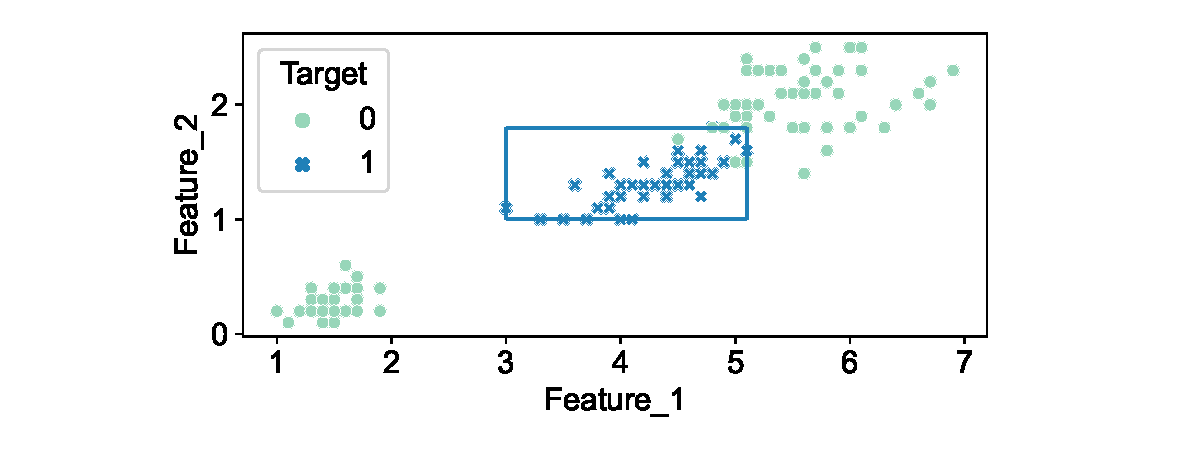
\includegraphics[width=\textwidth, trim=15 15 15 15, clip]{plots/csd-exemplary-subgroup.pdf}
	\caption{
		Exemplary subgroup description in the form of a rectangle for a dataset with two real-valued features and a binary prediction target.
	}
	\label{fig:csd:exemplary-subgroup}
\end{figure}

\paragraph{Subgroup discovery}

The goal of subgroup discovery is to find `interesting' subgroups, i.e., subsets of a dataset, like data objects where the prediction target takes a particular value~\cite{atzmueller2015subgroup}.
Additionally, such subgroups should be described with a combination of simple conditions on feature values, thereby fostering interpretability.
E.g., Figure~\ref{fig:csd:exemplary-subgroup} displays a rectangle-shaped subgroup description for a two-dimensional, real-valued dataset with a binary prediction target.
This subgroup is defined by $(\mathit{Feature\_1} \in [3.0, 5.1]) \land (\mathit{Feature\_2} \in [1.0, 1.8])$ and contains a considerably higher fraction of data objects with $\mathit{Target} = 1$ than the complete dataset.
One may see subgroup discovery as an extension of feature selection.
In particular, the result of subgroup discovery is not only a feature set but also comprises the value conditions.
Instead of training a prediction model with the selected feature set, the subgroup description implicitly forms a prediction model already.
In general, the subgroup description may define conditions on all features.
However, if it becomes too complex, i.e., involves too many features, its interpretability may decrease~\cite{meeng2021real}.
Thus, it makes sense to only use a subset of features in the subgroup description.

\section{Research Gaps}
\label{sec:introduction:research-gaps}

There are many existing methods for feature selection and subgroup discovery~\cite{atzmueller2015subgroup, li2017feature}.
However, we see two main research gaps where these two fields can be made more user-centric:
integrating domain knowledge and finding alternative solutions.
We will elaborate on these two points next.
Additionally, we will explain how we address both points with constraints on feature sets.

\subsection{Integrating Domain Knowledge}
\label{sec:introduction:research-gaps:integrating-domain-knowledge}

\paragraph{Motivation}

Most methods for feature selection and subgroup discovery optimize a quantitative quality criterion, e.g., a metric for prediction performance.
However, such approaches may yield suboptimal results from the user perspective, e.g., for interpreting the feature sets qualitatively.
In particular, these methods disregard domain knowledge about the dataset and its features.
Such domain knowledge is available in many scientific settings~\cite{karpatne2017theory, wagner2016theory}.
Users may want to consider different types of knowledge:
%
\begin{enumerate}
	\item
	\emph{Firm domain knowledge:}
	To make prediction models consistent with the domain, users may want them to adhere to known facts from the domain.
	For example, users may \emph{know} that some features are redundant from the domain perspective and thus want to rule out selecting combinations of these features.
	\item
	\emph{Hypotheses:}
	Hypotheses are ideas or expectations that users would like the selected feature sets to respect.
	For example, users may \emph{hypothesize} that certain features are redundant, and they want to study whether feature sets without these hypothesized redundancies suffice for predictions.
	If prediction performance drops significantly for feature sets respecting this hypothesis, the hypothesis may be wrong.
	\item
	\emph{Preferences:}
	Besides domain knowledge in the narrow sense, users may have further preferences on the selected feature sets.
	One example, which is already common in feature selection and subgroup discovery, is limiting the size of the feature sets.
	In particular, smaller feature sets may be easier to interpret.
\end{enumerate}

\paragraph{Problem and challenges}

In all previous scenarios, users want to limit the space of valid feature sets but not select individual feature sets manually.
Thus, we propose constraints on feature sets as a suitable approach to consider domain knowledge automatically.
We call the corresponding paradigms \emph{constrained feature selection} and \emph{constrained subgroup discovery}.
While observing constraints, we still want to optimize the quality of solutions, i.e., feature sets or subgroups.
The constraints may lower solution quality, but their exact impact is unclear a priori, and a certain decrease may still be acceptable for users.
Another central question is how to consider these constraints.
An ideal approach should support a wide range of constraints and their combination.
This flexibility gives users a lot of freedom, but it makes integration into existing methods for feature selection or subgroup discovery harder.
Also, the approach for integrating constraints should not be tied to one particular method.
I.e., we see the paradigm of constraints as orthogonal to existing methods.
However, the latter differ considerably in their objectives and internal structure, which poses a challenge for integrating constraints in a general fashion.

\paragraph{Related work}

Constraints have been used in many areas of data mining and machine learning~\cite{grossi2017survey}, e.g., automated machine learning~\cite{neutatz2023automl}, clustering \cite{dao2013declarative, dao2024review}, explainable AI~\cite{deutch2019constraints, gorji2022sufficient,  mothilal2020explaining, shrotri2022constraint}, and pattern mining \cite{ng1998exploratory, silva2016constrained}.
In feature selection, existing works tend to aim at just one feature-selection method and one constraint type, like group constraints \cite{friedman2010note, jacob2009group, simon2013sparse, yuan2006model, zhao2006grouped}, cost constraints \cite{jagdhuber2020cost, momeni2021cafs, paclik2002feature, plasberg2009feature, zhang2016learning}, or cardinality constraints \cite{khushaba2011feature, lee2018effective, serpico2001new, yang2015budget}.
Thus, there is potential for a more general approach to constrained feature selection.
In subgroup discovery, considering constraints is more common~\cite{atzmueller2015subgroup, meeng2021real}.
However, the subgroup-discovery methods that support constraints are typically limited to individual constraint types or at least require constraints to have particular properties, since the constraints need to be integrated into algorithmic search procedures.

\subsection{Finding Alternative Solutions}
\label{sec:introduction:research-gaps:finding-alternative-solutions}

\paragraph{Motivation}

Most methods for feature selection and subgroup discovery return only one solution, i.e., the optimum according to a quality criterion.
Nevertheless, there may be different solutions, i.e., using other features, that achieve similar quality.
Such alternative solutions are interesting for users, e.g., to obtain several diverse explanations.
In particular, alternatives can provide additional insights into predictions, enable users to develop and test different hypotheses, appeal to different kinds of users, and foster trust in the predictions~\cite{kim2021multi, wang2019designing}.
For example, in a dataset describing physical experiments, feature selection may help discover relationships between physical quantities.
If multiple alternative sets of similar quality exist, further analyses and experiments may be necessary to reveal the true underlying physical mechanism.
Only knowing one high-quality feature set and using it as the only explanation may be misleading in such a situation.

\paragraph{Problem and challenges}

We call our paradigms for finding alternative solutions \emph{alternative feature selection} and \emph{alternative subgroup description discovery}.
In the former case, we want to optimize feature-set quality; in the latter case, similarity regarding the set of data objects in the subgroup.
In both cases, constraints should enforce that the solutions are alternative in the sense of using different features.
For example, one can search for multiple solutions sequentially and require each new solution to optimize quality while being sufficiently dissimilar to previous solutions.
The constraints should be domain-independent since obtaining alternatives is a general concern and we want to free users from manually formulating corresponding constraint types.
However, users should have control over alternatives, e.g., their number and dissimilarity.
Depending on these user parameters, quality may drop, as with constraints in general, and users should decide on an acceptable quality trade-off.
Another recurring concern is to keep the approach for alternatives orthogonal to existing methods for feature selection and subgroup discovery.

\paragraph{Related work}

Only a few feature-selection methods return multiple, diverse feature sets~\cite{borboudakis2021extending}.
Existing approaches often do not guarantee diversity or do not give users control over diversity.
In fields related to feature selection, the goal of obtaining multiple, diverse solutions has been studied, e.g., for subspace clustering~\cite{hu2018subspace, mueller2009relevant}, subspace search~\cite{trittenbach2019dimension}, or explainable-AI techniques~\cite{artelt2022even, kim2016examples, mothilal2020explaining, russell2019efficient}.
These approaches are not directly applicable or easily adaptable to feature selection, and most of them provide limited or no user control.
In subgroup discovery, various methods yield a diverse set of subgroups~\cite{belfodil2019fssd, bosc2018anytime, leeuwen2012diverse, lemmerich2010fast, lucas2018ssdp+, proencca2022robust}.
However, this notion of alternatives typically aims to cover different subsets of data objects from the dataset.
In contrast, our notion of alternative subgroup descriptions aims to cover a similar set of data objects as in a given subgroup but with different features in the description.
Finally, for feature selection as well as subgroup discovery, existing work on alternatives typically proposes particular new search algorithms rather than an approach that is orthogonal to existing methods.

\section{Contributions}
\label{sec:introductions:contributions}

This dissertation provides four core contributions to make feature selection more user-centric with the help of constraints.
We address both research gaps from the previous section, i.e., integrating domain knowledge (cf.~Section~\ref{sec:introduction:research-gaps:integrating-domain-knowledge}) and finding alternative solutions (cf.~Section~\ref{sec:introduction:research-gaps:finding-alternative-solutions}).
Each core contribution corresponds to one chapter in the main part of this dissertation and may comprise several sub-contributions:

\paragraph{Evaluating the impact of constraints on feature-selection results (cf.~Chapter~\ref{sec:syn})}

First, we formalize constrained feature selection as an optimization problem.
Our problem definition is independent of the feature-selection method.
We also discuss how to solve this problem.
Second, we systematically analyze the impact of constraints.
To this end, we use datasets from various domains and generate random constraints.
A Satisfiability Modulo Theories (SMT) optimizer finds the optimal feature sets under these constraints.
Such a solver-based approach supports a wide range of constraint types.
We analyze the relationships between various evaluation metrics, describing the constraints and the feature-selection results.
Our experiments show that the impact of constraints strongly depends on the constraint type.
Additionally, we observe a nonlinear effect between the strength of constraints and feature-set quality:
Even if constraints prune a significant fraction of feature sets, the quality may not decrease to the same extent.

\paragraph{Formulating scientific hypotheses as constraints (cf.~Chapter~\ref{sec:ms})}

We conduct a case study in materials science to evaluate the impact of constraints for a concrete use case.
Here, we collaborate with domain experts to formulate constraints.
In particular, the constraints represent preferences and hypotheses from the domain.
We evaluate the hypotheses by analyzing how the corresponding constraints affect feature selection.
Our experiments show little variance in feature-set quality over the constraints, indicating that the data does not contradict the hypotheses.
However, the resulting feature sets differ in their composition, demonstrating that alternative solutions of similar quality exist.

\paragraph{Finding alternative feature sets (cf.~Chapter~\ref{sec:afs})}

First, we formalize alternative feature selection as an optimization problem.
In particular, we define alternatives via 0-1 integer linear constraints on feature sets.
Our approach is orthogonal to the feature-selection method and equips users with two parameters, i.e., the number of alternatives and a dissimilarity threshold.
For multiple alternatives, we consider sequential as well as simultaneous search.
Second, we discuss how to solve this optimization problem.
To that end, we describe how to integrate different categories of existing feature-selection methods into a solver-based search for alternatives.
Third, we analyze the time complexity of the optimization problem.
We show $\mathcal{NP}$-hardness, even for a simple notion of feature-set quality.
Fourth, we propose heuristic search methods that achieve a constant-factor approximation for a particular notion of feature-set quality.
Fifth, we conduct comprehensive experiments with five feature-selection methods, five search methods for alternatives, and varying the two user parameters.
Our experiments demonstrate that users can influence the quality of alternatives:
This quality tends to decrease for more alternatives and a higher dissimilarity threshold.
Runtime-wise, a solver-based sequential search for multiple alternatives is significantly faster than a simultaneous one while yielding a similar quality.
Additionally, our heuristic search methods yield a high quality in negligible runtime.

\paragraph{Discovering spare and alternative subgroup descriptions (cf.~Chapter~\ref{sec:csd})}

First, we formalize subgroup discovery as a Satisfiability Modulo Theories (SMT) optimization problem.
This formulation admits a solver-based search for subgroups and allows integrating constraints.
Second, we formalize two constraint types for this optimization problem.
\emph{Feature-cardinality constraints} limit the number of features used in subgroup descriptions.
\emph{Alternative subgroup descriptions} should use different features as a given subgroup description but cover a similar set of data objects.
Users control the number of alternatives and a dissimilarity threshold.
Third, we describe how to integrate these two constraint types into three existing heuristic search methods and two novel baselines for subgroup discovery.
Fourth, we analyze the time complexity of the subgroup-discovery problem with each of these two constraint types and prove several $\mathcal{NP}$-completeness results.
Fifth, we conduct comprehensive experiments with different experimental scenarios:
no constraints, feature-cardinality constraints, alternative subgroup descriptions, and different solver timeouts.
We observe that subgroups using only a few features already show relatively high quality compared to unconstrained subgroups.
With and without constraints, heuristic search methods yield similar subgroup quality as optimal solutions found by solver-based search, while being considerably faster.

\section{Materials}
\label{sec:introduction:materials}

We publish all code and experimental data for this dissertation under permissive licenses.

We provide the code, implemented in Python, via multiple \href{https://github.com/}{\emph{GitHub}} repositories, which we additionally backed up in the \href{https://archive.softwareheritage.org/}{\emph{Software Heritage archive}}:
%
\begin{itemize}
	\item Chapters~\ref{sec:syn} and~\ref{sec:ms}: \url{https://github.com/Jakob-Bach/Constrained-Filter-Feature-Selection} \newline
	Archived at \href{https://archive.softwareheritage.org/swh:1:dir:d94796f72c48b6f539cf528d0a8969b4ff61d42f;origin=https://github.com/Jakob-Bach/Constrained-Filter-Feature-Selection;visit=swh:1:snp:b9f0471bf7c5d1ee48572d687628ed14c786f901;anchor=swh:1:rev:77e893f8a6e42df004c999d009c2a02c8cdd9c5d}{swh:1:dir:d94796f72c48b6f539cf528d0a8969b4ff61d42f}
	\item Chapter~\ref{sec:afs}: \url{https://github.com/Jakob-Bach/Alternative-Feature-Selection} \newline
	Archived at \href{https://archive.softwareheritage.org/swh:1:dir:1e2b6605040a2151d31a90cde947787e92c98519;origin=https://github.com/Jakob-Bach/Alternative-Feature-Selection;visit=swh:1:snp:1413d85e1a9005d5681ee7dbeae0b4df851780de;anchor=swh:1:rev:14dea32227848c06b1430b6371e100f3d8c74010}{swh:1:dir:1e2b6605040a2151d31a90cde947787e92c98519}
	\item Chapter~\ref{sec:csd}: \url{https://github.com/Jakob-Bach/Constrained-Subgroup-Discovery} \newline
	Archived at \href{https://archive.softwareheritage.org/swh:1:dir:5527bcc4a86a1583e8bedf241f4738fc9b0e535c;origin=https://github.com/Jakob-Bach/Constrained-Subgroup-Discovery;visit=swh:1:snp:8f87dcdf0277985d373245e5a23a128efc861153;anchor=swh:1:rev:0c0e4a978c95d881c4c20eecdd5a1ae12ee08ac3}{swh:1:dir:5527bcc4a86a1583e8bedf241f4738fc9b0e535c}
\end{itemize}
%
We released all repositories under the \href{https://opensource.org/license/MIT}{MIT license}.
Each repository contains detailed instructions on how to reproduce the corresponding experiments.
Also, requirements files specify the versions of all dependencies.
Additionally, we organized all generally applicable functionality of each repository, e.g., methods for alternative feature selection, as a Python package to ease reuse.
The corresponding packages \href{https://pypi.org/project/alfese/}{\emph{alfese}}, \href{https://pypi.org/project/cffs/}{\emph{cffs}}, and \href{https://pypi.org/project/csd/}{\emph{csd}} are publicly available on \href{https://pypi.org}{\emph{PyPI}}.

We provide the experimental data via \href{https://radar.kit.edu}{\emph{RADAR4KIT}} and put it under the \href{https://creativecommons.org/licenses/by/4.0/}{CC-BY 4.0 license}: \url{https://doi.org/10.35097/4kjyeg0z2bxmr6eh}

\section{Prior Works}
\label{sec:introduction:prior-works}

This dissertation bases on the following preprints and publications:
%
\begin{itemize}
	\item \fullcite{bach2022empirical}
	\item \fullcite{bach2022leveraging}
	\item \fullcite{bach2023finding}
	\item \fullcite{bach2024alternative}
	\item \fullcite{bach2024using}
\end{itemize}
%
We have reused these prior works' content but revised it to form a coherent monograph.
In particular, these prior works contain all major contributions of this dissertation.
However, we have extended, rephrased, restructured, or shortened the text in various places.
Algorithms, definitions, equations, figures, notation, propositions, and tables in this dissertation may slightly differ from prior works, e.g., due to harmonization.
The four chapters in the main part of this dissertation explicitly state which prior works they base on.
All other chapters may reuse content from each of these prior works.

\section{Dissertation Outline}
\label{sec:introduction:outline}

The remainder of this dissertation is structured into three parts.

First, we present preliminaries.
Chapter~\ref{sec:fundamentals} describes relevant fundamentals of feature selection and subgroup discovery.
Chapter~\ref{sec:related-work} discusses related work for all our contributions.

The second part of this dissertation is the main part.
It consists of four chapters featuring our contributions.
Chapter~\ref{sec:syn} evaluates the impact of constraints on feature-selection results.
Chapter~\ref{sec:ms} presents a case study where constraints express scientific hypotheses.
Chapter~\ref{sec:afs} uses constraints to find alternative feature sets.
Chapter~\ref{sec:csd} employs constraints to discover sparse and alternative subgroup descriptions.

The third part of this dissertation wraps up our work.
Chapter~\ref{sec:conclusions} summarizes the conclusions, and Chapter~\ref{sec:future-work} discusses future work.
After the bibliography, Appendix~\ref{sec:appendix} contains proofs and technical details not included in the main part of this dissertation.

\chapter{Fundamentals}
\label{sec:fundamentals}

In this section, we introduce relevant fundamentals of feature selection (cf.~Section~\ref{sec:fundamentals:feature-selection}) and subgroup discovery (cf.~Section~\ref{sec:fundamentals:subgroup-discovery}).

\paragraph{Notation}

We focus on tabular, real-valued data.
In particular, $X \in \mathbb{R}^{m \times n}$ stands for a dataset in the form of a matrix.
Each row is a data object, and each column is a feature.
$\tilde{F} = \{f_1, \dots, f_n\}$ is the corresponding set of feature names.
We assume that categorical features have been made numeric, e.g., via a one-hot or an ordinal encoding~\cite{matteucci2023benchmark}.
$X_{i \cdot} \in \mathbb{R}^n$ denotes the values of all features for the $i$-th data object,
while $X_{\cdot j} \in \mathbb{R}^m$ denotes the values of the $j$-th feature for all data objects.
We consider supervised-learning scenarios.
In particular, the vector $y \in Y^m$ represents the prediction target with domain $Y$, e.g., $Y=\{0,1\}$ for binary classification or $Y=\mathbb{R}$ for regression.
The function $Q(\cdot)$ returns the quality of a feature set or subgroup; we will define its corresponding arguments later.

\section{Feature Selection}
\label{sec:fundamentals:feature-selection}

In this section, we introduce relevant fundamentals of feature selection:
the optimization problem (cf.~Section~\ref{sec:fundamentals:feature-selection:problem}) and feature-selection methods (cf.~Section~\ref{sec:fundamentals:feature-selection:methods}).

\subsection{Problem}
\label{sec:fundamentals:feature-selection:problem}

Feature selection makes a binary decision $s_j \in \{0,1\}$ for each feature, i.e., either selects it or not.
The vector $s \in \{0,1\}^n$ combines all these selection decisions and yields the selected feature set $F_s = \{f_j \mid s_j=1\} \subseteq \tilde{F}$.
To simplify notation, we drop the subscript~$s$ in definitions where we do not explicitly refer to the value of~$s$ but only the set~$F$.
The function $Q(s,X,y)$ returns the quality of such a feature set and depends on the feature-selection method.
Without loss of generality, we assume that this function should be maximized:
%
\begin{definition}[Feature selection]
	Given a dataset~$X \in \mathbb{R}^{m \times n}$ with prediction target~$y \in Y^m$,
	\emph{feature selection} is the problem of making feature-selection decisions~$s \in \{0,1\}^n$ that maximize a given notion of feature-set quality~$Q(s,X,y)$.
	\label{def:fs:feature-selection}
\end{definition}

Additionally, the user often defines a parameter $k \in \mathbb{N}$ denoting the exact or maximal number of selected features, i.e., the \emph{cardinality} of the feature set.

\subsection{Methods}
\label{sec:fundamentals:feature-selection:methods}

There are different ways to define feature-set quality $Q(s,X,y)$.
We only give a short overview and provide details for the methods we use in this dissertation. See~\cite{agrawal2021metaheuristic, chandrashekar2014survey, dhal2021comprehensive, li2017feature, njoku2023wrapper} for comprehensive studies and surveys of feature selection.
Feature-selection methods are typically categorized into filter, wrapper, and embedded methods~\cite{guyon2003introduction}.

\subsubsection{Filter Methods}
\label{sec:fundamentals:feature-selection:methods:filter}

Filter feature selection evaluates the quality $Q(s,X,y)$ without training a prediction model.
Univariate filters assess each feature's relevance independently.
Multivariate filters also consider relationships between features.
They often combine a measure of univariate feature relevance with a measure of bivariate feature redundancy.
Some filter methods also consider feature intercooperation, i.e., the joint relevance of two or more features~\cite{sosa2024feature}.

\paragraph{Univariate filter methods}

Univariate filter methods break $Q(s,X,y)$ down to the qualities $q_j = q(X_{\cdot{}j},y)$ of individual features.
$q(\cdot)$ is a bivariate dependency measure to quantify the relationship between each feature and the prediction target, e.g., mutual information~\cite{kraskov2004estimating} or the absolute value of Pearson correlation.
The overall optimization objective is an aggregate of the selected features' qualities, typically their sum:
%
\begin{equation}
	\max_s \quad Q_{\text{uni}}(s,X,y) = \sum_{j=1}^{n} q(X_{\cdot{}j},y) \cdot s_j = \sum_{j=1}^{n} q_j \cdot s_j
	\label{eq:fs:univariate-filter}
\end{equation}
%
This objective is cheap to compute but ignores interactions between features.
The optimal feature set of size~$k \in \mathbb{N}$ consists of the features with the $k$ highest individual qualities.

\paragraph{FCBF}

The Fast Correlation-Based Filter (FCBF)~\cite{yu2003feature} is a multivariate filter method that bases on the notion of predominance:
Each selected feature's correlation with the prediction target must exceed (1) a user-defined threshold and (2) the correlation of each other selected feature with the given one.
The first criterion ensures feature relevance, and the second criterion reduces feature redundancy.
\cite{yu2003feature} proposes a search algorithm to find a set of such predominant features.

\paragraph{mRMR}

Minimal Redundancy Maximal Relevance (mRMR)~\cite{peng2005feature} is a multivariate filter method that combines feature relevance and feature redundancy in one objective.
Relevance corresponds to the dependency between features and the prediction target, which should be maximized, as for univariate filters.
Redundancy, in turn, corresponds to the dependency between features, which should be minimized.
Both terms are averaged over the selected features.
Using a bivariate dependency measure~$q(\cdot)$, the objective is maximizing the following difference between relevance and redundancy:
%
\begin{equation}
	\max_s \quad Q_{\text{mRMR}}(s,X,y) = \frac{\sum_{j=1}^{n} q(X_{\cdot{}j},y) \cdot s_j}{\sum_{j=1}^{n} s_j} - \frac{\sum_{j_1=1}^{n} \sum_{j_2=1}^{n} q(X_{\cdot{}j_1}, X_{\cdot{}j_2}) \cdot s_{j_1} \cdot s_{j_2}}{(\sum_{j=1}^{n} s_j)^2}
	\label{eq:fs:mrmr}
\end{equation}

\subsubsection{Wrapper Methods}
\label{sec:fundamentals:feature-selection:methods:wrapper}

Wrapper methods~\cite{kohavi1997wrappers} evaluate feature-set quality~$Q(s,X,y)$ by training prediction models with feature sets and measuring prediction quality.
They employ a generic search strategy to iterate over candidate feature sets, e.g., genetic algorithms~\cite{agrawal2021metaheuristic}.
Feature-set quality is a black-box function in this search, i.e., the optimization algorithm only observes the objective's outputs rather than its internal structure.
On the one hand, the repeated model training makes wrapper methods costly.
On the other hand, the notion of feature-set quality stems from an actual prediction task rather than a simplified proxy objective.

\subsubsection{Embedded Methods}
\label{sec:fundamentals:feature-selection:methods:embedded}

Embedded methods train prediction models with built-in feature selection, e.g., decision trees~\cite{breiman1984classification} or random forests~\cite{breiman2001random}.
Thus, the criterion for feature-set quality is model-specific.
For example, tree-based models often use information gain or the Gini index to select features for creating the tree's decision nodes during training.

\subsubsection{Post-Hoc Feature-Importance Methods}
\label{sec:fundamentals:feature-selection:methods:importance}

Apart from conventional feature selection, there are various methods that assess feature importance after training a model.
These methods range from local explanation methods like LIME~\cite{ribeiro2016should} or SHAP~\cite{lundberg2017unified}, focusing on individual data objects, to global importance methods like permutation importance~\cite{breiman2001random} or SAGE~\cite{covert2020understanding}.
In particular, assessing feature importance plays a crucial role in the field of machine-learning interpretability~\cite{carvalho2019machine, molnar2020interpretable}.

\section{Subgroup Discovery}
\label{sec:fundamentals:subgroup-discovery}

In this section, we introduce relevant fundamentals of subgroup discovery:
the optimization problem (cf.~Section~\ref{sec:fundamentals:subgroup-discovery:problem}) and common heuristic search methods (cf.~Section~\ref{sec:fundamentals:subgroup-discovery:methods}).

\subsection{Problem}
\label{sec:fundamentals:subgroup-discovery:problem}

In general, subgroup discovery involves finding descriptions of interesting subsets of a dataset~\cite{atzmueller2015subgroup}.
There are multiple options for the type of dataset, kind of subgroup description, and criterion of interestingness.
In the following, we formalize the notion of subgroup discovery that we tackle in this dissertation.
For broader surveys, see~\cite{atzmueller2015subgroup, helal2016subgroup, herrera2011overview, ventura2018subgroup}.

\paragraph{Subgroup (description)}

A subgroup description typically comprises a conjunction of conditions on individual features~\cite{meeng2021real}.
For real-valued data, the conditions constitute intervals.
Thus, the subgroup description defines a hyperrectangle (cf.~Figure~\ref{fig:csd:exemplary-subgroup}) with a lower and upper bound for each feature.
The bounds for a feature may also be infinite to leave it unrestricted.
A data object resides in the subgroup if all its feature values are in the intervals formed by lower and upper bounds:
%
\begin{definition}[Subgroup (description)]
	Given a dataset~$X \in \mathbb{R}^{m \times n}$, a \emph{subgroup} is described by its lower bounds~$\mathit{lb} \in \{\mathbb{R} \cup \{-\infty, +\infty\}\}^n$ and upper bounds~$\mathit{ub} \in \{\mathbb{R} \cup \{-\infty, +\infty\}\}^n$.
	Data object $X_{i \cdot}$ is a \emph{member} of this subgroup if $\forall j \in \{1, \dots, n\}:~ \left( X_{ij} \geq \mathit{lb}_j \right) \land \left( X_{ij} \leq \mathit{ub}_j \right)$.
	\label{def:csd:subgroup}
\end{definition}
%
While we focus on real-valued data, some subgroup-discovery methods only support categorical data and require continuous features to be discretized~\cite{herrera2011overview, meeng2021real}.
In this case, the inequality comparisons become equality comparisons against feature values~\cite{atzmueller2015subgroup}.

Throughout this dissertation, we often use the terms \emph{subgroup} and \emph{subgroup description} interchangeably.
In a more strict sense, the former term denotes the subgroup's members, and the latter denotes the subgroup's bounds~\cite{atzmueller2015subgroup}.

\paragraph{Subgroup discovery}

Subgroup discovery sets the bounds $\mathit{lb}$ and $\mathit{ub}$ to optimize a notion of subgroup quality~$Q(\mathit{lb}, \mathit{ub}, X, y)$, i.e., the interestingness of the subgroup.
To harmonize formalization and evaluation, we focus on binary-classification targets~$y \in \{0,1\}^m$.
In general, one may also conduct subgroup discovery in multi-class, multi-target, or regression scenarios~\cite{atzmueller2015subgroup}.
Without loss of generality, we assume a maximization problem:
%
\begin{definition}[Subgroup discovery]
	Given a dataset~$X \in \mathbb{R}^{m \times n}$ with prediction target $y \in \{0, 1\}^m$,
	\emph{subgroup discovery} is the problem of finding a subgroup (cf.~Definition~\ref{def:csd:subgroup}) with bounds~$\mathit{lb}, \mathit{ub} \in \{\mathbb{R} \cup \{-\infty, +\infty\}\}^n$ that maximizes a given notion of subgroup quality $Q(\mathit{lb}, \mathit{ub}, X, y)$.
	\label{def:csd:subgroup-discovery}
\end{definition}
%
While this definition refers to one subgroup, some methods return a subgroup set~\cite{atzmueller2015subgroup}.

\paragraph{Subgroup quality}

For binary targets, interesting subgroups should typically contain many data objects from one class but few from the other.
Without loss of generality, we assume that the class with label~`1' is the class of interest, also called \emph{positive} class.
Weighted Relative Accuracy (WRAcc)~\cite{lavravc1999rule} is a popular metric for subgroup quality~\cite{meeng2021real}:
%
\begin{equation}
	\text{WRAcc} = \frac{m_b}{m} \cdot \left( \frac{m_b^+}{m_b} - \frac{m^+}{m} \right)
	\label{eq:csd:wracc}
\end{equation}
%
Besides the total number of data objects~$m$, this metric considers the number of positive data objects~$m^+$, the number of data objects in the subgroup~$m_b$, and the number of positive data objects in the subgroup~$m_b^+$.
In particular, WRAcc is the product of two factors:
$m_b / m$ expresses the generality of the subgroup as the relative frequency of subgroup membership.
The second factor measures the relative accuracy of the subgroup, i.e., the difference in the relative frequency of the positive class between the subgroup and the whole dataset.
If the subgroup contains the same fraction of positive data objects as the whole dataset, WRAcc is zero.
The theoretical maximum and minimum of WRAcc depend on the class frequencies in the dataset.
In particular, the maximum WRAcc for a dataset equals the product of the relative frequencies of positive and negative data objects in the dataset~\cite{mathonat2021anytime}:
%
\begin{equation}
	\text{WRAcc}_{\text{max}} = \frac{m^+}{m} \cdot \left( 1 - \frac{m^+}{m} \right)
	\label{eq:csd:wracc-max}
\end{equation}
%
This maximum is reached if all positive data objects are in the subgroup and all negative ones are outside, i.e., $m_b^+ = m_b = m^+$.
The corresponding value is 0.25 if both classes occur with equal frequency but becomes smaller the more imbalanced the classes are.
Thus, it makes sense to normalize WRAcc when working with datasets with different class frequencies.
One option is a max-normalization to the range $[-1, 1]$~\cite{mathonat2021anytime}:
%
\begin{equation}
	\text{nWRAcc} = \frac{\text{WRAcc}}{\text{WRAcc}_{\text{max}}} = \frac{m_b^+ \cdot m - m^+ \cdot m_b}{m^+ \cdot (m - m^+)}
	\label{eq:csd:wracc-normalized}
\end{equation}
%
Alternatively, one can also min-max-normalize the range to~$[0, 1]$~\cite{carmona2018unifying, ventura2018subgroup}.

\subsection{Methods}
\label{sec:fundamentals:subgroup-discovery:methods}

There are heuristic search methods to discover subgroups, like PRIM~\cite{friedman1999bump} and Best Interval~\cite{mampaey2012efficient}, as well as exhaustive search methods, like SD-Map~\cite{atzmueller2009fast, atzmueller2006sd}, MergeSD~\cite{grosskreutz2009subgroup}, and BSD~\cite{lemmerich2016fast, lemmerich2010fast}.
In this section, we discuss three heuristic search methods that are relevant for Chapter~\ref{sec:csd}; see~\cite{atzmueller2015subgroup, helal2016subgroup, herrera2011overview, ventura2018subgroup} for comprehensive surveys.

\begin{algorithm}[t]
	\DontPrintSemicolon
	\KwIn{Dataset~$X \in \mathbb{R}^{m \times n}$, \newline
		Prediction target~$y \in \{0, 1\}^m$, \newline
		Subgroup-quality function~$Q(\mathit{lb}, \mathit{ub}, X, y)$, \newline
		Peeling fraction~$\alpha \in (0, 1)$, \newline
		Support threshold~$\beta_0 \in [0, 1]$
	}
	\KwOut{Subgroup bounds~$\mathit{lb}, \mathit{ub} \in \{\mathbb{R} \cup \{-\infty, +\infty\}\}^n$}
	\BlankLine
	\For(\tcp*[f]{Start with unrestricted subgroup}){$j \leftarrow 1$ \KwTo $n$}{ \label{al:csd:prim:line:initialization-start}
		$(\mathit{lb}^{\text{opt}}_j,~ \mathit{ub}^{\text{opt}}_j) \leftarrow (-\infty, +\infty)$\;
	}
	$Q^{\text{opt}} \leftarrow Q(\mathit{lb}^{\text{opt}}, \mathit{ub}^{\text{opt}}, X, y)$\;
	$(\mathit{lb}^{\text{peel}}, \mathit{ub}^{\text{peel}}) \leftarrow (\mathit{lb}^{\text{opt}},~ \mathit{ub}^{\text{opt}})$\; \label{al:csd:prim:line:initialization-end}
	\While(\tcp*[f]{Support threshold satisfied}){$\frac{m_b}{m} > \beta_0$}{ \label{al:csd:prim:line:stop} \label{al:csd:prim:iteration-start}
		$Q^{\text{cand}} \leftarrow -\infty$\;
		\For{$j \in$ get\_permissible\_feature\_idxs(\dots)}{ \label{al:csd:prim:line:peel-start} \label{al:csd:prim:line:permissible-features}
			$(\mathit{lb},~ \mathit{ub}) \leftarrow (\mathit{lb}^{\text{peel}},~ \mathit{ub}^{\text{peel}})$ \tcp*{Try peeling lower bound}
			$\mathit{lb}_j \leftarrow$ quantile($X_{\cdot j}$, $\mathit{lb}$, $\mathit{ub}$, $\alpha$)\;
			\If{$Q(\mathit{lb}, \mathit{ub}, X, y) > Q^{\text{cand}}$}{
				$(\mathit{lb}^{\text{cand}}, \mathit{ub}^{\text{cand}}) \leftarrow (\mathit{lb}, \mathit{ub})$\;
			}
			$(\mathit{lb},~ \mathit{ub}) \leftarrow (\mathit{lb}^{\text{peel}},~ \mathit{ub}^{\text{peel}})$ \tcp*{Try peeling upper bound}
			$\mathit{ub}_j \leftarrow$ quantile($X_{\cdot j}$, $\mathit{lb}$, $\mathit{ub}$, $1-\alpha$)\;
			\If{$Q(\mathit{lb}, \mathit{ub}, X, y) > Q^{\text{cand}}$}{
				$(\mathit{lb}^{\text{cand}}, \mathit{ub}^{\text{cand}}) \leftarrow (\mathit{lb}, \mathit{ub})$\; \label{al:csd:prim:line:peel-end}
			}
		}
		$(\mathit{lb}^{\text{peel}}, \mathit{ub}^{\text{peel}}) \leftarrow (\mathit{lb}^{\text{cand}}, \mathit{ub}^{\text{cand}})$ \tcp*{Retain best candidate} \label{al:csd:prim:line:best-peel-selection}
		\If(\tcp*[f]{Update optimum}){$Q(\mathit{lb}^{\text{peel}}, \mathit{ub}^{\text{peel}}, X, y) > Q^{\text{opt}}$}{ \label{al:csd:prim:line:opt-check-start}
			$Q^{\text{opt}} \leftarrow Q(\mathit{lb}^{\text{peel}}, \mathit{ub}^{\text{peel}}, X, y)$\;
			$(\mathit{lb}^{\text{opt}},~ \mathit{ub}^{\text{opt}}) \leftarrow (\mathit{lb}^{\text{peel}},~ \mathit{ub}^{\text{peel}})$\; \label{al:csd:prim:line:opt-check-end} \label{al:csd:prim:iteration-end}
		}
	}
	$(\mathit{lb}, \mathit{ub}) \leftarrow (\mathit{lb}^{\text{opt}}, \mathit{ub}^{\text{opt}})$\; \label{al:csd:prim:line:select-optimal-bounds}
	\For(\tcp*[f]{Reset non-excluding bounds}){$j \leftarrow 1$ \KwTo $n$}{ \label{al:csd:prim:line:bounds-infty-start}
		\lIf{$\mathit{lb}_j = \min_{i \in \{1, \dots, m\}} X_{ij}$}{$\mathit{lb}_j \leftarrow -\infty$}
		\lIf{$\mathit{ub}_j = \max_{i \in \{1, \dots, m\}} X_{ij}$}{$\mathit{ub}_j \leftarrow +\infty$} \label{al:csd:prim:line:bounds-infty-end}
	}
	\Return{$\mathit{lb}, \mathit{ub}$}
	\caption{\emph{PRIM} for subgroup discovery.}
	\label{al:csd:prim}
\end{algorithm}

\paragraph{PRIM}

\emph{Patient Rule Induction Method (PRIM)}~\cite{friedman1999bump} is an iterative search algorithm.
Its basic form consists of a peeling phase and a pasting phase.
Peeling restricts the bounds of the subgroup iteratively, while pasting expands them.
Algorithm~\ref{al:csd:prim} outlines the peeling phase for finding one subgroup, which is the flavor of PRIM we consider in this dissertation and denote as \emph{PRIM}.
Pasting may have little effect on the subgroup quality and is often left out~\cite{arzamasov2021reds}.
Other extensions of PRIM are bumping~\cite{friedman1999bump, kwakkel2016improving}, which uses bagging of multiple PRIM runs to improve subgroup quality, and covering~\cite{friedman1999bump}, which returns a sequence of subgroups covering different data objects.

The algorithm \emph{PRIM} starts with a subgroup containing all data objects, which is the initial solution candidate (Lines~\ref{al:csd:prim:line:initialization-start}--\ref{al:csd:prim:line:initialization-end}).
It continues peeling until the current solution candidate contains at most a fraction~$\beta_0$ of data objects (Line~\ref{al:csd:prim:line:stop}).
The support threshold~$\beta_0 \in [0, 1]$ is a user parameter.
The returned subgroup is the optimal solution candidate over all peeling iterations (Line~\ref{al:csd:prim:line:select-optimal-bounds}).
In our \emph{PRIM} implementation, we additionally set \emph{non-excluding bounds} to infinity (Lines~\ref{al:csd:prim:line:bounds-infty-start}--\ref{al:csd:prim:line:bounds-infty-end}).
These are bounds that do not exclude any data objects from the subgroup, i.e., equal the minimum/maximum feature value over all data objects.
Thereby, we ensure that these bounds remain non-excluding for any new data and make it easier to see which features are selected in the subgroup description (cf.~Definition~\ref{def:csd:feature-selection}).

In the iterative peeling procedure (Lines~\ref{al:csd:prim:iteration-start}--\ref{al:csd:prim:iteration-end}), the algorithm generates new solution candidates by trying to restrict each \emph{permissible feature} (Lines~\ref{al:csd:prim:line:peel-start}--\ref{al:csd:prim:line:peel-end}).
By default, each feature is permissible, but the function \emph{get\_permissible\_feature\_idxs(\dots)} will become helpful once we introduce constraints.
For each Feature~$j$, the algorithm tests a new lower bound at the $\alpha$-quantile of feature values in the subgroup and a new upper bound at the $1-\alpha$-quantile of feature values in the subgroup.
The peeling fraction $\alpha \in (0, 1)$ is a user parameter.
It describes which fraction of data objects gets excluded from the subgroup in each peeling iteration.
Having tested two new bounds for each feature, the algorithm takes the subgroup with the highest associated quality (Line~\ref{al:csd:prim:line:best-peel-selection}) and continues peeling it in the next iteration.
Further, if this solution candidate improves upon the optimal solution candidate from all prior iterations, it is stored as the new optimum (Lines~\ref{al:csd:prim:line:opt-check-start}--\ref{al:csd:prim:line:opt-check-end}).

\begin{algorithm}[t]
	\DontPrintSemicolon
	\KwIn{Dataset~$X \in \mathbb{R}^{m \times n}$, \newline
		Prediction target~$y \in \{0, 1\}^m$, \newline
		Subgroup-quality function~$Q(\mathit{lb}, \mathit{ub}, X, y)$, \newline
		Beam width~$w \in \mathbb{N}$
	}
	\KwOut{Subgroup bounds~$\mathit{lb}, \mathit{ub} \in \{\mathbb{R} \cup \{-\infty, +\infty\}\}^n$}
	\BlankLine
	\For(\tcp*[f]{Initialize beam}){$l \leftarrow 1$ \KwTo $w$}{ \label{al:csd:generic-beam-search:line:initialization-start}
		\For{$j \leftarrow 1$ \KwTo $n$}{
			$(\mathit{lb}^{(\text{beam, } l)}_j,~ \mathit{ub}^{(\text{beam, } l)}_j) \leftarrow (-\infty, +\infty)$ \tcp*{Unrestricted}
		}
		$\mathit{cand\_has\_changed}^{(l)} \leftarrow$ \textbf{true} \tcp*{Subgroup should be updated}
		$Q^{(l)} \leftarrow Q(\mathit{lb}^{(\text{beam, } l)}, \mathit{ub}^{(\text{beam, } l)}, X, y)$\; \label{al:csd:generic-beam-search:line:initialization-end}
	}
	\While(\tcp*[f]{Beam has changed}){$\left( \sum_{l=1}^w \mathit{cand\_has\_changed}^{(l)} \right) > 0$}{ \label{al:csd:generic-beam-search:line:iteration-start} \label{al:csd:generic-beam-search:line:stop}
		$\mathit{prev\_cand\_changed\_idxs} \leftarrow \{l \mid \mathit{cand\_has\_changed}^{(l)} \}$\;
		\For(\tcp*[f]{Create temporary solution candidates}){$l \leftarrow 1$ \KwTo $w$}{
			$(\mathit{lb}^{(\text{cand, } l)},~ \mathit{ub}^{(\text{cand, } l)}) \leftarrow$ $(\mathit{lb}^{(\text{beam, } l)},~ \mathit{ub}^{(\text{beam, } l)})$\;
			$\mathit{cand\_has\_changed}^{(l)} \leftarrow$ \textbf{false}\;
		}
		\For(\tcp*[f]{Prepare beam updates}){$l \in \mathit{prev\_cand\_changed\_idxs}$}{ \label{al:csd:generic-beam-search:line:update-start}
			\For{$j \in$ get\_permissible\_feature\_idxs(\dots)}{ \label{al:csd:generic-beam-search:line:permissible-features}
				evaluate\_subgroup\_updates(\dots) \tcp*{Algorithm~\ref{al:csd:beam-search-subgroup-update} or~\ref{al:csd:best-interval-subgroup-update}} \label{al:csd:generic-beam-search:line:update-end}
			}
		}
		\For(\tcp*[f]{Update beam}){$l \leftarrow 1$ \KwTo $w$}{
			$(\mathit{lb}^{(\text{beam, } l)},~ \mathit{ub}^{(\text{beam, } l)}) \leftarrow$ $(\mathit{lb}^{(\text{cand, } l)},~ \mathit{ub}^{(\text{cand, } l)})$\; \label{al:csd:generic-beam-search:line:iteration-end}
		}
	}
	$l \leftarrow \arg\max_{l \in \{1, \dots, w\}} Q^{(l)}$ \tcp*{Select best subgroup from beam} \label{al:csd:generic-beam-search:line:finalization-start}
	$(\mathit{lb},~ \mathit{ub}) \leftarrow (\mathit{lb}^{(\text{beam, } l)},~ \mathit{ub}^{(\text{beam, } l)})$\;
	\For(\tcp*[f]{Reset non-excluding bounds}){$j \leftarrow 1$ \KwTo $n$}{ \label{al:csd:generic-beam-search:line:bounds-infty-start}
		\lIf{$\mathit{lb}_j = \min_{i \in \{1, \dots, m\}} X_{ij}$}{$\mathit{lb}_j \leftarrow -\infty$}
		\lIf{$\mathit{ub}_j = \max_{i \in \{1, \dots, m\}} X_{ij}$}{$\mathit{ub}_j \leftarrow +\infty$} \label{al:csd:generic-beam-search:line:bounds-infty-end}
	}
	\Return{$\mathit{lb}, \mathit{ub}$}  \label{al:csd:generic-beam-search:line:finalization-end}
	\caption{Generic beam search for subgroup discovery.}
	\label{al:csd:generic-beam-search}
\end{algorithm}

\begin{algorithm}[t]
	\DontPrintSemicolon
	\KwIn{Parameters and variables from Algorithm~\ref{al:csd:generic-beam-search}}
	\KwOut{None; modifies variables from Algorithm~\ref{al:csd:generic-beam-search} in-place}
	$(\mathit{lb},~ \mathit{ub}) \leftarrow (\mathit{lb}^{(\text{beam, } l)},~ \mathit{lb}^{(\text{beam, } l)})$ \tcp*{Next, update lower bound} \label{al:csd:beam-search-subgroup-update:line:lb-start}
	\For{$b \in $ sort(unique(get\_feature\_values($X$, $j$, $\mathit{lb}^{(\text{beam, } l)}$, $\mathit{ub}^{(\text{beam, } l)}$)))}{
		$\mathit{lb}_j \leftarrow b$\;
		\If{$\left( Q(\mathit{lb}, \mathit{ub}, X, y) > \min_{l \in \{1, ..., w\}} Q^{(l)} \right)$ \textbf{and} $(\mathit{lb},~ \mathit{ub}) \notin \{(\mathit{lb}^{(\text{cand, } l)},~ \mathit{ub}^{(\text{cand, } l)}) \mid l \in \{1, \dots, w\}\}$ }{ \label{al:csd:beam-search-subgroup-update:line:lb-replace-start}
			$l \leftarrow \arg\min_{l \in \{1, \dots, w\}} Q^{(l)}$ \tcp*{Replace worst candidate}
			$(\mathit{lb}^{(\text{cand, } l)},~ \mathit{ub}^{(\text{cand, } l)}) \leftarrow (\mathit{lb}, \mathit{ub})$\;
			$\mathit{cand\_has\_changed}^{(l)} \leftarrow$ \textbf{true}\;
			$Q^{(l)} \leftarrow Q(\mathit{lb}, \mathit{ub}, X, y)$\; \label{al:csd:beam-search-subgroup-update:line:lb-replace-end} \label{al:csd:beam-search-subgroup-update:line:lb-end}
		}
	}
	$(\mathit{lb},~ \mathit{ub}) \leftarrow (\mathit{lb}^{(\text{beam, } l)},~ \mathit{lb}^{(\text{beam, } l)})$ \tcp*{Next, update upper bound} \label{al:csd:beam-search-subgroup-update:line:ub-start}
	\For{$b \in $ sort(unique(get\_feature\_values($X$, $j$, $\mathit{lb}^{(\text{beam, } l)}$, $\mathit{ub}^{(\text{beam, } l)}$)))}{
		$\mathit{ub}_j \leftarrow b$\;
		\If{$\left( Q(\mathit{lb}, \mathit{ub}, X, y) > \min_{l \in \{1, ..., w\}} Q^{(l)} \right)$ \textbf{and} $(\mathit{lb},~ \mathit{ub}) \notin \{(\mathit{lb}^{(\text{cand, } l)},~ \mathit{ub}^{(\text{cand, } l)}) \mid l \in \{1, \dots, w\}\}$ }{ \label{al:csd:beam-search-subgroup-update:line:ub-replace-start}
			$l \leftarrow \arg\min_{l \in \{1, \dots, w\}} Q^{(l)}$ \tcp*{Replace worst candidate}
			$(\mathit{lb}^{(\text{cand, } l)},~ \mathit{ub}^{(\text{cand, } l)}) \leftarrow (\mathit{lb}, \mathit{ub})$\;
			$\mathit{cand\_has\_changed}^{(l)} \leftarrow$ \textbf{true}\;
			$Q^{(l)} \leftarrow Q(\mathit{lb}, \mathit{ub}, X, y)$\; \label{al:csd:beam-search-subgroup-update:line:ub-replace-end} \label{al:csd:beam-search-subgroup-update:line:ub-end}
		}
	}
	\caption{evaluate\_subgroup\_updates(\dots) for \emph{Beam Search}.}
	\label{al:csd:beam-search-subgroup-update}
\end{algorithm}

\paragraph{Beam Search}

Beam search is a generic search strategy that is also common in subgroup discovery~\cite{atzmueller2005exploiting}.
It maintains a set of currently best solution candidates, i.e., the beam, which it iteratively updates.
The number of solution candidates in the beam is a user parameter, i.e., the beam width~$w \in \mathbb{N}$.
We outline our specific implementation, which we denote as \emph{Beam Search}, in Algorithm~\ref{al:csd:generic-beam-search} combined with Algorithm~\ref{al:csd:beam-search-subgroup-update}.
It is an adapted version of the beam-search implementation in the Python package \emph{pysubgroup}~\cite{lemmerich2019pysubgroup}.

First, the algorithm \emph{Beam Search} initializes the beam by creating $w$ unrestricted subgroups (Lines~\ref{al:csd:generic-beam-search:line:initialization-start}--\ref{al:csd:generic-beam-search:line:initialization-end}).
Further, it stores the quality of each of these subgroups.
Additionally, it records which subgroups changed in the previous iteration (Lines~\ref{al:csd:generic-beam-search:line:iteration-start}--\ref{al:csd:generic-beam-search:line:iteration-end}) of the search.
In particular, it stops once all subgroups in the beam remain unchanged (Line~\ref{al:csd:generic-beam-search:line:stop}).
Subsequently, it returns the best subgroup from the beam (Lines~\ref{al:csd:generic-beam-search:line:finalization-start}--\ref{al:csd:generic-beam-search:line:finalization-end}).
As for \emph{PRIM} (cf.~Algorithm~\ref{al:csd:prim}), we replace all non-excluding bounds with infinity as a post-processing step.

The main loop (Lines~\ref{al:csd:generic-beam-search:line:iteration-start}--\ref{al:csd:generic-beam-search:line:iteration-end}) updates the beam.
In particular, for each subgroup that changed in the previous iteration, the algorithm creates new solution candidates by attempting to update the bounds of each feature separately (Lines~\ref{al:csd:generic-beam-search:line:update-start}--\ref{al:csd:generic-beam-search:line:update-end}).
There are different options for this update step.
Algorithm~\ref{al:csd:beam-search-subgroup-update} outlines the specific update procedure for \emph{Beam Search}, while \emph{Best Interval} uses a slightly different one (cf.~Algorithm~\ref{al:csd:best-interval-subgroup-update}).
For \emph{Beam Search}, the procedure tries to refine either the lower bound (Lines~\ref{al:csd:beam-search-subgroup-update:line:lb-start}--\ref{al:csd:beam-search-subgroup-update:line:lb-end}) or the upper bound (Lines~\ref{al:csd:beam-search-subgroup-update:line:ub-start}--\ref{al:csd:beam-search-subgroup-update:line:ub-end}) for a given Feature~$j$.
In particular, all unique feature values from data objects in the subgroup may act as new bounds.
Each solution candidate that improves upon the minimum subgroup quality from the beam replaces the corresponding subgroup, unless it already is part of the beam due to another update action (Lines~\ref{al:csd:beam-search-subgroup-update:line:lb-replace-start}--\ref{al:csd:beam-search-subgroup-update:line:lb-replace-end} and~\ref{al:csd:beam-search-subgroup-update:line:ub-replace-start}--\ref{al:csd:beam-search-subgroup-update:line:ub-replace-end}).

\begin{algorithm}[t]
	\DontPrintSemicolon
	\KwIn{Parameters and variables from Algorithm~\ref{al:csd:generic-beam-search}}
	\KwOut{None; modifies variables from Algorithm~\ref{al:csd:generic-beam-search} in-place}
	$(\mathit{lb},~ \mathit{ub}) \leftarrow (\mathit{lb}^{(\text{beam, } l)},~ \mathit{lb}^{(\text{beam, } l)})$ \tcp*{Value at index~$j$ will change}  \label{al:csd:best-interval-subgroup-update:line:main-start}
	$(\mathit{lb}^{\text{opt}},~ \mathit{ub}^{\text{opt}}) \leftarrow (\mathit{lb}^{(\text{beam, } l)},~ \mathit{lb}^{(\text{beam, } l)})$ \tcp*{$(l, r)$ in~\cite{mampaey2012efficient}}
	$Q^{\text{opt}} \leftarrow Q(\mathit{lb}^{\text{opt}}, \mathit{ub}^{\text{opt}}, X, y)$ \tcp*{$\textit{WRAcc}_{\text{max}}$ in~\cite{mampaey2012efficient}}
	$Q^{\text{temp}} \leftarrow -\infty$ \tcp*{$h_{\text{max}}$ in~\cite{mampaey2012efficient}}
	$\mathit{lb}^{\text{temp}}_j \leftarrow -\infty$ \tcp*{$t_{\text{max}}$ in~\cite{mampaey2012efficient}}
	\For{$b \in $ sort(unique(get\_feature\_values($X$, $j$, $\mathit{lb}^{(\text{beam, } l)}$, $\mathit{ub}^{(\text{beam, } l)}$)))}{
		$\mathit{lb}_j \leftarrow b$\;
		$\mathit{ub}_j \leftarrow \mathit{ub}^{(\text{beam, } l)}_j$\;
		\If{$Q(\mathit{lb}, \mathit{ub}, X, y) > Q^{\text{temp}}$}{
			$\mathit{lb}^{\text{temp}}_j \leftarrow b$\;
			$Q^{\text{temp}} \leftarrow Q(\mathit{lb}, \mathit{ub}, X, y)$\;
		}
		$\mathit{lb}_j \leftarrow \mathit{lb}^{\text{temp}}_j$\;
		$\mathit{ub}_j \leftarrow b$\;
		\If{$Q(\mathit{lb}, \mathit{ub}, X, y) > Q^{\text{opt}}$}{
			$(\mathit{lb}^{\text{opt}},~ \mathit{ub}^{\text{opt}}) \leftarrow (\mathit{lb},~ \mathit{ub})$\;
			$Q^{\text{opt}} \leftarrow Q(\mathit{lb}, \mathit{ub}, X, y)$\; \label{al:csd:best-interval-subgroup-update:line:main-end}
		}
	}
	\If{$\left( Q^{\text{opt}} > \min_{l \in \{1, ..., w\}} Q^{(l)} \right)$ \textbf{and} $(\mathit{lb}^{\text{opt}},~ \mathit{ub}^{\text{opt}}) \notin \{(\mathit{lb}^{(\text{cand, } l)},~ \mathit{ub}^{(\text{cand, } l)}) \mid l \in \{1, \dots, w\}\}$ }{ \label{al:csd:best-interval-subgroup-update:line:replace-start}
		$l \leftarrow \arg\min_{l \in \{1, \dots, w\}} Q^{(l)}$ \tcp*{Replace worst candidate}
		$(\mathit{lb}^{(\text{cand, } l)},~ \mathit{ub}^{(\text{cand, } l)}) \leftarrow (\mathit{lb}^{\text{opt}}, \mathit{ub}^{\text{opt}})$\;
		$\mathit{cand\_has\_changed}^{(l)} \leftarrow$ \textbf{true}\;
		$Q^{(l)} \leftarrow Q^{\text{opt}}$\; \label{al:csd:best-interval-subgroup-update:line:replace-end}
	}
	\caption{evaluate\_subgroup\_updates(\dots) for \emph{Best Interval}.}
	\label{al:csd:best-interval-subgroup-update}
\end{algorithm}

\paragraph{Best Interval}

\emph{Best Interval}~\cite{mampaey2012efficient} offers an update procedure for subgroups (cf.~Algorithm~\ref{al:csd:best-interval-subgroup-update}) that is tailored towards WRAcc (cf.~Equation~\ref{eq:csd:wracc}) as the subgroup-quality function.
This update procedure can be used within a generic beam-search strategy (cf.~Algorithm~\ref{al:csd:generic-beam-search}).
As before, a solution candidate from an update step becomes part of the beam if it improves upon the worst subgroup quality there and is not a duplicate (Lines~\ref{al:csd:best-interval-subgroup-update:line:replace-start}--\ref{al:csd:best-interval-subgroup-update:line:replace-end} in Algorithm~\ref{al:csd:best-interval-subgroup-update}).

However, solution candidates are generated differently than in the update procedure of \emph{Beam Search} (cf.~Algorithm~\ref{al:csd:beam-search-subgroup-update}).
In particular, \emph{Best Interval} updates lower and upper bounds for a given Feature~$j$ simultaneously rather than separately (Lines~\ref{al:csd:best-interval-subgroup-update:line:main-start}--\ref{al:csd:best-interval-subgroup-update:line:main-end} in Algorithm~\ref{al:csd:best-interval-subgroup-update}).
Thus, this procedure optimizes over all potential combinations of lower and upper bounds.
However, it still only requires one pass over the unique values of Feature~$j$ rather than quadratic cost, as it leverages theoretical properties of the WRAcc function~\cite{mampaey2012efficient}.

\chapter{Related Work}
\label{sec:related-work}

In this chapter, we discuss related work.
We organize this discussion according to the two main research gaps we address (cf.~Section~\ref{sec:introduction:research-gaps}):
Section~\ref{sec:related-work:constraints} covers approaches for integrating constraints and domain knowledge, while Section~\ref{sec:related-work:alternatives} examines approaches for finding alternative solutions.
In both sections, we elaborate on the fields of feature selection and subgroup discovery in detail before reviewing other related fields.

\section{Integrating Constraints and Domain Knowledge}
\label{sec:related-work:constraints}

In this section, we discuss related work on considering constraints and domain knowledge in feature selection
(cf.~Section~\ref{sec:related-work:constraints:feature-selection}), subgroup discovery
(cf.~Section~\ref{sec:related-work:constraints:subgroup-discovery}), and other related fields
(cf.~Section~\ref{sec:related-work:constraints:other-fields}).
Constraints for finding alternatives follow in Section~\ref{sec:related-work:alternatives}.

\subsection{Feature Selection}
\label{sec:related-work:constraints:feature-selection}

\paragraph{Constraint types and approaches}

Despite the number and variety of existing feature-selection methods (cf.~Section~\ref{sec:fundamentals:feature-selection:methods}), considering constraints and domain knowledge is less well-researched.
Existing work typically has a narrower scope than ours since it tends to focus only on one feature-selection method and one constraint type rather than pursuing a more general approach.
There is work on cost constraints~\cite{jagdhuber2020cost, momeni2021cafs, paclik2002feature, plasberg2009feature, zhang2016learning} and cardinality constraints~\cite{khushaba2011feature, lee2018effective, serpico2001new, yang2015budget}.
Feature selection with predefined groups of features has been studied as well, though mainly specific to linear prediction models, e.g., group lasso and its variants~\cite{friedman2010note, jacob2009group, simon2013sparse, yuan2006model, zhao2006grouped}.
As a more general work, \cite{groves2015toward}~presents four wrapper-feature-selection methods that can theoretically support arbitrary constraint types.
However, their evaluation only employs a narrow set of constraint types, related to lagged temporal features or a hierarchy of feature groups.
Also, their wrapper approaches treat constraints as a black box, i.e., they only check whether constraints are satisfied and correspondingly exclude invalid candidate feature sets from the search.
In contrast, we primarily use white-box solvers to consider constraints in the optimization.
\cite{neutatz2021enforcing}~introduces a wrapper approach supporting arbitrary constraint types and feature-selection methods.
However, they also implement constraints as black-box functions.
Apart from feature-set size, their constraints do not refer to feature sets per se but metrics for the whole machine-learning system, e.g., accuracy, fairness, or training time.
Further, the constraints are not integrated into feature selection but are checked after training and evaluating a prediction model with the selected features.

\paragraph{Other notions of constrained feature selection}

Some subfields of data mining refer to `constraints' in combination with `feature selection' but mean different problems than we do.
First, feature selection with constraints is studied in semi-supervised learning~\cite{hijazi2021active, rostami2020novel, sheikhpour2017survey, zhang2008constraint}.
However, the constraints there express relationships between data objects, not between features.
For example, constraints may state whether two data objects belong to the same class, without assigning a class label.
Second, constraints play a role in unsupervised feature selection~\cite{lu2018unsupervised, zhang2019nonlinear, zhang2020unsupervised}.
These constraints do not directly express user needs on feature sets but help find a low-dimensional representation of the data.
Third, there is constraint-based feature selection that builds on Bayesian network learning~\cite{lagani2017feature}.
It does not involve user-defined constraints but conditional independence constraints between features, which are automatically learned and propagated.

\subsection{Subgroup Discovery}
\label{sec:related-work:constraints:subgroup-discovery}

\paragraph{White-box formulations}

To consider constraints in subgroup discovery, we provide an SMT formulation of the problem (cf.~Section~\ref{sec:csd:approach:smt}) and tackle it with a corresponding solver.
To our knowledge, this formulation is novel.
There are a few other white-box formulations of particular variants of subgroup discovery, e.g., constraint-programming formulations of \textsc{Discriminative Itemset Mining}~\cite{guns2011itemset, koccak2020exploiting} and \textsc{Relevant Subgroup Discovery}~\cite{koccak2020exploiting}, and integer-programming formulations of the \textsc{Maximum Box} problem~\cite{eckstein2002maximum}, \textsc{Maximum $\alpha$-Pattern} problem~\cite{bonates2008maximum}, and the \textsc{Box Search} problem~\cite{louveaux2014combinatorial}.
Additionally, there are also white-box formulations for other prediction models~\cite{ignatiev2021reasoning} that share some similarities with subgroup descriptions, e.g., formulations in propositional logic (SAT) for decision trees, decision sets, and decision lists~\cite{narodytska2018learning, shati2021sat, yu2021learning}.
All previously mentioned works address different problem definitions than we do, e.g., use additional constraints but not the specific constraint types we analyze.
Also, their evaluations differ from ours.
For example, they do not compare against existing heuristic subgroup-discovery methods.

\paragraph{Constraint types}

There is work on considering different constraint types in subgroup discovery.
Typically, constraints are integrated into algorithmic search methods rather than formulated declaratively for solver-based optimization.
\cite{meeng2021real} mentions three common constraint types:
lower bounds on subgroup quality, lower bounds on the number of subgroup members, and upper bounds on the search depth.
The latter influences the number of features used.
Several subgroup-discovery methods employ quality-based pruning to reduce the search space, e.g., using optimistic estimates in exhaustive search~\cite{atzmueller2015subgroup, atzmueller2009fast, grosskreutz2009subgroup}.
However, such automatically determined bounds on subgroup quality are not user-defined constraints.
\cite{atzmueller2006methodological, atzmueller2005exploiting, atzmueller2007using} provide a taxonomy and examples for knowledge-based constraint types in subgroup discovery.
\cite{atzmueller2007using}~expresses domain knowledge declaratively with the logic programming language Prolog but does not use a solver for optimization.

\paragraph{Feature-cardinality constraints}

Feature-cardinality constraints (cf.~Definition~\ref{def:csd:feature-cardinality-constraint}) are one of the two constraint types we analyze in Chapter~\ref{sec:csd}.
While feature cardinality is a well-known metric for subgroup complexity~\cite{helal2016subgroup, herrera2011overview, ventura2018subgroup}, our SMT formulation of this constraint type is novel.
\cite{li2015efficient}~formulates a quadratic program to select non-redundant features for subgroups, but with real-valued feature weights as decision variables and only as a subroutine within an algorithmic search.
Two alternatives to feature-cardinality constraints are constraints~\cite{lavrac2006relevancy} or post-processing~\cite{friedman1999bump} to eliminate irrelevant features.

Several works on subgroup discovery use a feature-cardinality constraint in their experiments~\cite{arzamasov2022pedagogical, lavrac2006relevancy, leeuwen2012diverse, leeuwen2013discovering, mampaey2012efficient}, but there is a lack of studies that analyze the impact of different feature-cardinality thresholds on different subgroup-discovery methods broadly and systematically.
\cite{friedman1999bump, lemmerich2010fast, proencca2022robust} compare multiple feature-cardinality thresholds for one subgroup-discovery method each, while \cite{helal2016subgroup} compares multiple subgroup-discovery methods for one feature-cardinality threshold.
\cite{meeng2021real} evaluates three subgroup-discovery methods and four feature-cardinality thresholds but mainly focuses their evaluation on comparing strategies for handling numeric data.
Also, they use fewer and lower-dimensional datasets than we do.
Further, they do not compare to an unconstrained setting.

\subsection{Other Fields}
\label{sec:related-work:constraints:other-fields}

\paragraph{Data mining and machine learning}

Besides feature selection and subgroup discovery, working with constraints is a research area for various subfields of data mining and machine learning \cite{grossi2017survey}, e.g., automated machine learning~\cite{neutatz2023automl}, clustering \cite{dao2013declarative, dao2024review}, explainable AI~\cite{deutch2019constraints, gorji2022sufficient, mothilal2020explaining, shrotri2022constraint}, and pattern mining \cite{ng1998exploratory, silva2016constrained}.
There is also work in the other direction, i.e., using machine-learning techniques in constraint solving~\cite{popescu2022overview}.

\paragraph{Materials science}

Since we conduct a case study on constrained feature selection in materials science (cf.~Chapter~\ref{sec:ms}), we also review related work in this field.
In materials science, various feature-selection methods have already been applied~\cite{agrawal2014exploration, imbalzano2018automatic, janet2017resolving}, but without considering constraints.
At the same time, researchers argue for the integration of domain knowledge in machine learning~\cite{mangal2018comparative, wagner2016theory}.
To this end, \cite{childs2019embedding, ramprasad2017machine} survey machine-learning approaches in materials science, some of which use domain knowledge when creating new features rather than when selecting them.
For example, physical laws can guide which interaction terms should be created from the original features.
As another example, `fingerprint' feature vectors for describing materials have implicit physical constraints on feature values~\cite{huan2015accelerated}.
Apart from constraints, one can directly involve domain experts in feature selection.
\cite{liu2020multi} lets domain experts rate the importance of features and combines these manual ratings with several automated feature-selection steps.
Such an approach requires domain knowledge about the usefulness of individual features, while our constraints express knowledge about the relationships between features.

\paragraph{Software engineering}

There are approaches for constrained feature selection in software engineering~\cite{benavides2010automated, galindo2019automated, harman2014search}.
Despite technical similarities, the semantics of \emph{feature} and \emph{feature-set quality} differ from our work, which limits the comparability of empirical studies.

A \emph{feature} in software engineering is a characteristic of a software product, not a column in a tabular dataset (cf.~Section~\ref{sec:fundamentals:feature-selection:problem}).
\emph{Feature selection} then aims at configuring a software system, which may even be a machine-learning system~\cite{aloisio2023democratizing}.
\emph{Feature models} express logical relationships, i.e., constraints, between features, often forming a hierarchical structure.
Further, \emph{feature attributes} express properties like component costs, memory requirements, etc.
These properties form the base for further constraints or one or several target functions \cite{guo2011genetic, henard2015combining, sayyad2013value}.
Typical approaches to find feature sets include sampling \cite{oh2017finding}, constraint solving \cite{white2010automated}, adapting general-purpose optimization techniques \cite{guo2011genetic}, and combining satisfiability solving with general-purpose optimization~\cite{guo2014scaling, guo2019smtibea, henard2015combining}.

Empirical studies on feature selection in software engineering often use feature models with predefined constraints from repositories like LVAT \cite{lvat} and SPLOT \cite{mendonca2009splot}.
Only some works also generate constrained feature models for a more systematic evaluation.
\cite{guo2011genetic, ochoa2019constraint, thum2009reasoning} iteratively generate constraints, randomly picking constraint types and the features to be used, similar to our study with random constraints (cf.~Chapter~\ref{sec:syn}).
However, these works use generated constraints to evaluate new approaches for dealing with constraints, while we focus on evaluating the impact of constraints themselves.

\section{Finding Alternative Solutions}
\label{sec:related-work:alternatives}

In this section, we discuss related work on finding alternative solutions in feature selection
(cf.~Section~\ref{sec:related-work:alternatives:feature-selection}), subgroup discovery
(cf.~Section~\ref{sec:related-work:alternatives:subgroup-discovery}), and other related fields
(cf.~Section~\ref{sec:related-work:alternatives:other-fields}).

\subsection{Feature Selection}
\label{sec:related-work:alternatives:feature-selection}

\paragraph{Conventional feature selection}

Most feature-selection methods only yield one solution~\cite{borboudakis2021extending}, though some exceptions exist~\cite{emmanouilidis1999selecting, mueller2021feature, siddiqi2020genetic}.
However, none of the cited approaches searches for alternatives in our sense.
For example, they pursue different objectives and give users less control, e.g., do not guarantee the dissimilarity of alternatives.

\paragraph{Ensemble feature selection}

Ensemble feature selection~\cite{saeys2008robust, seijo2017ensemble} combines feature-selection results, e.g., obtained by different feature-selection methods or on different samples of the data.
Fostering diverse feature sets may be a sub-goal to improve prediction performance~\cite{guru2018alternative, liu2019subspace, shekar2017diverse, woznica2012model}, but it is usually only an intermediate step.
This focus differs from our notion of alternative feature sets, and users have less control over alternatives.

\paragraph{Statistically equivalent feature sets}

Methods for statistically equivalent feature sets~\cite{borboudakis2021extending, lagani2017feature} use statistical tests to determine features or feature sets that are equivalent for predictions.
Our notion of alternatives differs in several aspects.
In particular, building optimal alternatives from equivalent feature sets is not straightforward.
There can be arbitrarily many equivalent feature sets, without an explicit quality-based ordering, while we provide a user-defined number of alternatives.
Also, our alternatives need not have equivalent quality but should be optimal under constraints.
Further, our dissimilarity threshold allows controlling the overlap between sets instead of eliminating all redundancies.

\subsection{Subgroup Discovery}
\label{sec:related-work:alternatives:subgroup-discovery}

To our knowledge, alternative subgroup descriptions in the sense of this dissertation (cf.~Definition~\ref{def:csd:alternative-subgroup-description-discovery}) are a novel concept.
In particular, we \emph{maximize} the set similarity of contained data objects relative to a given subgroup while using a different subgroup description.
In contrast, various existing approaches strive for alternatives in the sense of diverse or non-redundant sets of subgroups, which \emph{minimize} the overlap of contained data objects without constraints on the description.
After presenting such techniques for \emph{subgroup-set selection}, we discuss approaches focusing on subgroup descriptions.

\paragraph{Subgroup-set selection}

Since subgroups only cover specific regions of the data, it is natural to search for multiple subgroups to cover multiple regions; see~\cite{atzmueller2015subgroup} for an overview of subgroup-set selection.
The \emph{covering} approach supports any subgroup-discovery method by removing all data objects contained in previous subgroups and repeating subgroup discovery~\cite{friedman1999bump}.
Alternatively, one may reweigh~\cite{gamberger2002expert, lavrac2004subgroup} or resample~\cite{scholz2005sampling} data objects based on their subgroup membership.
Other subgroup-discovery methods specifically search for multiple solutions simultaneously~\cite{leeuwen2012diverse, leeuwen2013discovering, lemmerich2010fast, lucas2018ssdp+, proencca2022robust}.
The notion of subgroup quality then typically goes beyond predictive quality like WRAcc and involves metrics for the diversity~\cite{belfodil2019fssd, leeuwen2012diverse, leeuwen2013discovering, lucas2018ssdp+} and number~\cite{helal2016subgroup, herrera2011overview, ventura2018subgroup} of subgroups.
One may also filter redundant subgroups as a post-processing step~\cite{bosc2018anytime, grosskreutz2012enhanced, hudson2023subgroup, leeuwen2013discovering}.

\paragraph{Description-based diverse subgroup-set selection}

\cite{leeuwen2012diverse} introduces six strategies to foster diversity between subgroups.
Two strategies refer to subgroup descriptions:
The first excludes subgroup descriptions that have the same quality and differ in only one condition from an existing subgroup description.
The second uses a global upper bound on how often a feature may be selected in a set of subgroup descriptions.
Both these strategies give users less control over the overlap of subgroup descriptions than we do.
Further, \cite{leeuwen2012diverse} optimizes subgroup quality in a simultaneous beam search.
In contrast, we search for alternative descriptions sequentially, optimize similarity to the original subgroup, and consider a solved-based search method in addition to heuristic search.

\paragraph{Diverse top-k characteristics lists}

\cite{lopez2023discovering}~introduces the notion of \emph{diverse top-k characteristic lists}, which is a set of lists, each containing multiple patterns, e.g., subgroups.
Within each list, the subgroups should be diverse in terms of data objects contained.
Further, exactly the same subgroup description must not appear in two lists.
However, any other partial overlap of descriptions is allowed, which is less specific than our definition.

\paragraph{Equivalent subgroup descriptions of minimal length}

\cite{boley2009non}~introduces the notion of \emph{equivalent subgroup descriptions of minimal length}, which is stricter than our notion of alternative subgroup descriptions.
In particular, the former descriptions need to cover exactly the same set of data objects instead of maximizing similarity.
Further, a subset of the original feature set should be found, instead of using a different feature set subject to a dissimilarity constraint.
The authors prove $\mathcal{NP}$-hardness, which influenced our proof of Proposition~\ref{prop:csd:complexity-cardinality-np-perfect-subgroup}, and propose two algorithms for their problem but do not pursue a solver-based search.

\paragraph{Redescription mining}

Redescription mining aims to find pairs or sets of descriptions that cover exactly or approximately the same data objects~\cite{galbrun2017redescription, ramakrishnan2004turning}.
We pursue a similar goal but search for alternative descriptions sequentially instead of simultaneously.
Also, we have a target variable while redescription mining is unsupervised~\cite{ramakrishnan2004turning}.
Further, redescription mining works with different feature-set dissimilarity criteria than we do~\cite{galbrun2017redescription, gallo2008finding, mihelcic2023complexity, parida2005redescription}, and the language for redescriptions may be more complex than for subgroups~\cite{galbrun2017redescription, gallo2008finding}.
Finally, most existing approaches for redescription mining are algorithmic rather than using white-box optimization~\cite{galbrun2017redescription, mihelcic2023complexity}, though~\cite{guns2013kpattern} provides a constraint-programming formulation.
\cite{mihelcic2023complexity} shows that several variants of redescription mining are $\mathcal{NP}$-hard.

\subsection{Other Fields}
\label{sec:related-work:alternatives:other-fields}

\paragraph{Clustering}

Finding alternative solutions has been addressed extensively in the field of clustering. \cite{bailey2014alternative} gives a taxonomy and describes corresponding algorithms.
On a high level, this work inspired our notions of alternatives in feature selection and subgroup discovery.
Nevertheless, the concrete problem definitions for alternatives are fundamentally different.
First, the notion of dissimilarity differs, as we focus on feature sets rather than limiting the assignments of data objects to clusters~\cite{bae2006coala, bae2010clustering}.
Second, using constraints is only one of several approaches to obtain alternative clusterings.
Third, we are in a supervised prediction scenario (cf.~Section~\ref{sec:fundamentals}) while clustering is unsupervised.

\paragraph{Subspace clustering and subspace search}

Finding multiple feature sets is part of subspace clustering~\cite{gunnemann2009detection, hu2018subspace, mueller2009relevant} and subspace search~\cite{fouche2021efficient, nguyen20134s, trittenbach2019dimension}.
These approaches strive to improve the results of data-mining algorithms by using subspaces, i.e., feature sets, rather than all features.
Some approaches explicitly try to remove redundancy between subspaces~\cite{gunnemann2009detection, hu2018subspace, nguyen20134s} or foster subspace diversity~\cite{fouche2021efficient, trittenbach2019dimension}.
However, these subspace approaches differ from alternative feature selection and alternative subgroup descriptions in at least one of the following aspects:
First, they pursue different optimization objectives, e.g., a different notion of quality.
Second, definitions of subspace redundancy may consider data objects and feature values instead of only binary feature-selection decisions.
Third, users may have less control over the dissimilarity of alternatives, e.g., only a regularization parameter rather than a hard threshold.

\paragraph{Explainable artificial intelligence (XAI)}

Alternative explanations in XAI can provide additional insights into predictions, enable users to develop and test different hypotheses, appeal to different kinds of users, and foster trust in the predictions~\cite{kim2021multi, wang2019designing}.
In contrast, significantly different explanations for the same prediction may raise doubts about how meaningful the explanations are~\cite{jain2019attention}.
Finding diverse explanations has been studied for various explainers, e.g., for counterfactuals~\cite{dandl2020multi, karimi2020model, mohammadi2021scaling, mothilal2020explaining, russell2019efficient, wachter2017counterfactual}, criticisms~\cite{kim2016examples}, and semifactual explanations~\cite{artelt2022even}.
There are several approaches to foster diversity, e.g., ensembling different kinds of explanations~\cite{silva2019produce}, considering multiple local minima~\cite{wachter2017counterfactual}, using a search algorithm that maintains diversity~\cite{dandl2020multi}, extending the optimization objective~\cite{artelt2022even, kim2016examples, mothilal2020explaining}, or introducing constraints~\cite{karimi2020model, mohammadi2021scaling, russell2019efficient}.
Of the various mentioned approaches, only~\cite{artelt2022even, mohammadi2021scaling, mothilal2020explaining} introduce a parameter to control the diversity of solutions.
Of these three works, only~\cite{mohammadi2021scaling} offers a user-friendly dissimilarity threshold in~$[0,1]$, while the other two approaches employ a regularization parameter in the objective.

Despite similarities, the previously mentioned XAI techniques tackle different problems than we do.
In particular, they provide local explanations, i.e., aim at predictions for individual data objects, while we focus on the global quality of feature sets.
For example, counterfactual explanations~\cite{guidotti2022counterfactual, stepin2021survey, verma2020counterfactual} alter feature \emph{values} \emph{as little as possible} to produce an alternative prediction \emph{outcome}.
In contrast, alternative feature sets might alter the feature \emph{selection} \emph{significantly} while trying to maintain the original prediction \emph{quality}.

\paragraph{Rashomon sets}

A Rashomon set is a set of prediction models that reach a certain, e.g., close-to-optimal, prediction performance~\cite{fisher2019all}.
Despite similar performance, these models may still assign different feature importance scores, leading to different explanations~\cite{laberge2023partial}.
Thus, Rashomon sets may yield partial information about alternative feature sets.
However, approaches for Rashomon sets do not explicitly search for alternative feature sets as a whole but focus on the range of each feature's importance over prediction models.
Further, our notion of alternatives is broader, as it is not tied to model-based feature importance.

\paragraph{Number partitioning}

Special cases of alternative feature selection resemble existing number-partitioning problems from theoretical computer science.
Several restrictions of our problem are necessary to draw this connection, e.g., univariate feature-set quality and each feature being selected exactly once (cf.~Section~\ref{sec:afs:approach:complexity:univariate}).
Without restricting set sizes, a corresponding problem is called \textsc{Multi-Way Number Partitioning} or \textsc{Multiprocessor Scheduling}.
It has multiple problem formulations~\cite{garey2003computers, korf2010objective, lawrinenko2017identical}, $\mathcal{NP}$-hardness results~\cite{garey2003computers, korf2009multi}, parameterized-complexity results~\cite{mnich2018parameterized}, exact algorithms~\cite{haouari2008maximizing, schreiber2018optimal, walter2017improved}, and approximation algorithms~\cite{alon1998approximation, deuermeyer1982scheduling, sahni1976algorithms, woeginger1997polynomial}.
When restricting the set sizes, a related problem is called \textsc{Balanced Number Partitioning} or \textsc{K-Partitioning}.
Again, there are $\mathcal{NP}$-hardness results~\cite{babel1998thek, he2003kappa} as well as approximation algorithms~\cite{chen2016efficient, kellerer2011a32approximation, lawrinenko2018reduction, michiels2012computer, zhang2011heuristic}.
Our $\mathcal{NP}$-hardness results and approximation algorithms for univariate alternative feature selection (cf.~Section~\ref{sec:afs:approach}) build on these existing works.
However, alternative feature selection generally has a much broader scope than number partitioning, allowing for more sophisticated objectives, additional parametrization options, and evaluation with prediction scenarios rather than only summing numbers.


\chapter{Evaluating the Impact of Constraints on Feature-Selection Results}
\label{sec:syn}

\section{Overview}
\label{sec:syn:overview}

\paragraph{Scope}

Building on the motivation provided in Section~\ref{sec:introduction:research-gaps}, this chapter lays the foundations for constrained feature selection in general.
In contrast, the subsequent three chapters will focus on specific constraint types.
Besides formally introducing constrained feature selection, this chapter empirically evaluates the impact of constraints.
Generally, adding constraints may lower feature-set quality.
An important question is if there are sweet spots, i.e., high-quality feature sets that satisfy the constraints.

\paragraph{Contributions}

Our contribution in this chapter is twofold:

(1) We formalize constrained feature selection as an optimization problem and discuss how to solve it.
Our problem definition is independent of the feature-selection method.

(2) We conduct a systematic, domain-independent study to analyze the impact of constraints on feature-selection results.
To this end, we propose an experimental design that enables such an analysis.
In particular, we use 35 regression datasets from various domains and generate random constraints systematically.
We vary the constraint types, number of constraints, and features used.
Further, we define evaluation metrics that quantify the constraints and the feature-selection results.
We then empirically evaluate the relationships between these metrics.
We find optimal feature sets with a Satisfiability Modulo Theories (SMT) solver, which supports a broad range of constraint types.
In particular, we use univariate filter feature selection as the objective and formulate constraints in propositional logic and linear arithmetic.
Section~\ref{sec:syn:evaluation:summary} summarizes key results.

\paragraph{Materials}

We publish all our code and experimental data online (cf.~Section~\ref{sec:introduction:materials}).

\paragraph{Prior works}

The content of this chapter bases on the following prior work:
%
\begin{itemize}
	\item \fullcite{bach2022empirical}
\end{itemize}

\paragraph{Chapter outline}

The remainder of this chapter is structured as follows:
Section~\ref{sec:syn:approach} describes and analyzes constrained feature selection.
Section~\ref{sec:syn:experimental-design} outlines our experimental design.
Section~\ref{sec:syn:evaluation} presents the corresponding experimental results.

\section{Constrained Feature Selection}
\label{sec:syn:approach}

In this section, we introduce the problem of constrained feature selection.
After briefly defining the overall optimization problem (cf.~Section~\ref{sec:syn:approach:problem}), we describe potential constraints (cf.~Section~\ref{sec:syn:approach:constraints}) and how to consider them (cf.~Section~\ref{sec:syn:approach:optimization}).
Finally, we discuss the time complexity of this problem (cf.~Section~\ref{sec:syn:approach:complexity}).

\subsection{Optimization Problem}
\label{sec:syn:approach:problem}

For constrained feature selection, we keep the objective and decision variables of conventional feature selection (cf.~Definition~\ref{def:fs:feature-selection}).
I.e., we still optimize the feature-set quality~$Q(s,X,y)$ for a dataset~$X \in \mathbb{R}^{m \times n}$ and a prediction target~$y \in Y^m$ by making feature-selection decisions~$s \in \{0, 1\}^n$.
Thus, the general concept of constrained feature selection is independent of the feature-selection method, which determines the objective~$Q(s,X,y)$.
The novelty is admitting a set~$C$ of user-defined constraints for this optimization problem.
Each constraint $c \in C$ maps the feature-selection decisions~$s$ to true (1) or false (0).
We assume hard constraints, i.e., a valid feature set needs to satisfy all constraints:
%
\begin{equation}
	\begin{aligned}
		\max_s &\quad Q(s,X,y) \\
		\text{subject to:} &\quad \forall c \in C:~ c(s) = 1 \\
		\text{with:} &\quad C \subseteq \{c \mid c: \{0,1\}^n \to \{0, 1\}\}
	\end{aligned}
	\label{eq:syn:cfs-problem}
\end{equation}
%
The full textual problem definition corresponding to Equation~\ref{eq:syn:cfs-problem} is the following:
%
\begin{definition}[Constrained feature selection]
	Given a dataset~$X \in \mathbb{R}^{m \times n}$ with prediction target~$y \in Y^m$, and a set of constraints $C \subseteq \{c \mid c: \{0,1\}^n \to \{0, 1\}\}$,
	\emph{constrained feature selection} is the problem of making feature-selection decisions~$s \in \{0,1\}^n$ that maximize a given notion of feature-set quality~$Q(s,X,y)$ while satisfying all constraints, i.e., ${\forall c \in C:}~ c(s) = 1$.
	\label{def:syn:constrained-feature-selection}
\end{definition}

\subsection{Constraints}
\label{sec:syn:approach:constraints}

There is a broad range of possible constraint types.
Limiting the feature-set size to a user-defined cardinality~$k \in \mathbb{N}$, as common in many existing feature-selection methods, is only one possible constraint type.
In general, users should ultimately decide which constraint types to employ.
However, depending on the optimization method (cf.~Section~\ref{sec:syn:approach:optimization}), it makes sense to limit the categories of admissible constraint types, e.g., by prescribing particular logics to formulate constraints.
Such a limitation still offers more flexibility than only allowing one particular constraint type, as common in related work (cf.~Section~\ref{sec:related-work:constraints:feature-selection}).
In our work, we admit arbitrary constraints in propositional logic and linear arithmetic.
These two categories are domain-independent and allow the formulation of various expressive constraint types.
In particular, all constraint types in our domain-specific case study (cf.~Chapter~\ref{sec:ms}) can be formulated that way.
Additionally, propositional logic and linear arithmetic subsume typical constraint types from related work (cf.~Chapter~\ref{sec:related-work:constraints}).
Finally, these logics allow using a white-box solver for optimization (cf.~Section~\ref{sec:syn:approach:optimization}).

\paragraph{Propositional constraints}

Propositional constraints describe relationships between features with propositional logic.
The binary selection decisions $s_j \in \{0,1\}$ correspond to the logical values $\{\text{false}, \text{true}\}$.
One can now use logical operators like AND~($\land$), inclusive OR~($\lor$), exclusive OR~($\oplus$), NOT~($\lnot$), IMPLIES~($\rightarrow$), and IFF~($\leftrightarrow$).
For example, $s_1 \rightarrow s_2$ means that if Feature~1 is selected, then Feature~2 has to be selected as well.
By combining the operators, one can describe more complex relationships.
For example, $(s_4 \land s_7 \land s_{10}) \oplus (s_2 \land s_{11})$ means that either the three features from the first group or the two features from the second group have to be selected.

\paragraph{Arithmetic constraints}

The theory of linear arithmetic supports four operators~\cite{barrett2018satisfiability}:
addition~($+$), subtraction~($-$), multiplication~($\cdot$), and less-or-equal~($\leq$).
In the terminology of first-order logic, the first three operators are functions, returning another arithmetic value, while the inequality is a predicate, yielding a logical value.
Linear arithmetic does not allow multiplying two variables, as at least one operand has to be a constant~\cite{barrett2018satisfiability}.
In general, one can use linear-arithmetic constraints by assigning each feature a numeric value and formulating an inequality.
For example, suppose that each feature has a weight~$w_j \in \mathbb{R}_{\geq 0}$, e.g., measurement cost, and one wants to select a feature set with a total weight below a threshold $w_{\text{max}} \in \mathbb{R}_{> 0}$.
This yields the following linear inequality: 
%
\begin{equation}
	\sum_{j=1}^n s_j \cdot w_j \leq w_{\text{max}}
\end{equation}

For instance, such a situation occurs if feature values are obtained with sensors with different energy consumption, and the total amount of energy per measurement is limited.

A cardinality constraint on the feature-set size is a special case of a weighted-sum constraint.
It has uniform weights and a desired minimum, exact, or maximum cardinality~$k \in \mathbb{N}$:
%
\begin{equation}
	\sum_{j=1}^n s_j = k
	\label{eq:syn:cardinality}
\end{equation}

One may use propositional and arithmetic constraints interchangeably in some situations.
Think of a group of five features, and one wants to select at least one of them.
Arithmetically, the sum of selection decisions for these five features should be at least one.
With propositional logic, one may employ the OR~($\lor$) operator.

\subsection{Optimization Methods}
\label{sec:syn:approach:optimization}

Depending on the formulation of the constrained optimization problem, different optimization methods are suitable.
Conventional feature-selection methods are typically not designed to operate in a constrained search space; they support a cardinality constraint at most.
Adapting individual feature-selection methods to individual constraint types is feasible in some cases but lacks generality.
Instead, we propose to use a generic white-box or black-box optimizer to tackle constrained feature selection.

White-box optimizers consider the internal structure of the optimization problem.
In particular, they must support formulating the chosen objective and constraint types.
Nevertheless, they provide more flexibility than adapting existing feature-selection methods since they typically support a broad range of expressions.
In particular, they allow users to combine arbitrary constraints within the supported logic declaratively.

In contrast, black-box optimization methods only process the objective value without knowing how its function is defined.
This characteristic increases generality but also means that some information about the internals of the optimization problem remains unused.
In some cases, constraint types may be black-box functions as well.

Our chapter on alternative feature selection (cf.~Section~\ref{sec:afs:approach:objectives}) provides a detailed discussion on white-box and black-box optimization for different feature-selection methods.
In the current chapter's experiments, we use univariate filter feature selection (cf.~Equation~\ref{eq:fs:univariate-filter}) as the optimization objective.
This simple linear objective is independent of the prediction model and allows us to use an off-the-shelf white-box solver to find optimal feature sets.
In particular, we employ a Satisfiability Modulo Theories (SMT) optimizer~\cite{barrett2018satisfiability}.
Such solvers support constraints in propositional logic and first-order theories like arithmetic, bit vectors, or arrays.
We already decided to formulate constraints in propositional logic and linear arithmetic (cf.~Section~\ref{sec:syn:approach:constraints}), which fits the scope of SMT.
The objective function in Equation~\ref{eq:fs:univariate-filter} is also linear once the feature qualities~$q(X_{\cdot{}j},y)$ are computed.

If all constraints are in propositional logic, then the optimization problem with this objective becomes a weighted \textsc{Max One} problem~\cite{khanna1997complete}.
This is a special case of a weighted partial maximum satisfiability (\textsc{MaxSAT}) problem~\cite{bacchus2021maximum, li2021maxsat}, where the individual binary decision variables form the soft clauses for optimization and the user-defined constraints constitute the hard clauses.
Such a problem formulation gives way to specialized \textsc{MaxSAT} solvers.
If we include arithmetic constraints, the formulation is a \textsc{MaxSMT} problem~\cite{nieuwenhuis2006sat}.

\subsection{Time Complexity}
\label{sec:syn:approach:complexity}

We analyze three aspects of time complexity for constrained feature selection:
the size of the search space for exhaustive search, parameterized complexity, and $\mathcal{NP}$-hardness.
While the results here are relatively straightforward, they also lay the foundation for further complexity analyses regarding alternative feature selection (cf.~Section~\ref{sec:afs:approach:complexity}) and constrained subgroup discovery (cf.~Sections~\ref{sec:csd:approach:cardinality:complexity} and~\ref{sec:csd:approach:alternatives:complexity}).

\paragraph{Exhaustive search}

Without constraints, the search space of feature selection grows exponentially with the number of features~$n$.
In particular, there are $2^n - 1$ possibilities to form a non-empty feature set of arbitrary size.
In the worst case, finding the optimal feature set requires iterating over this entire space.
In practice, particular notions of feature-set quality may allow finding the optimum faster, or a feature-selection method may only strive for an approximate solution.

Constraints can reduce the search space, but the upper bound remains the same:
%
\begin{proposition}[Complexity of exhaustive search for (constrained) feature selection]
	An exhaustive search for feature selection with or without constraints (cf.~Definitions~\ref{def:fs:feature-selection} and~\ref{def:syn:constrained-feature-selection}) needs to evaluate $O(2^n)$ feature sets.
	\label{prop:syn:complexity-constrained-exhaustive}
\end{proposition}
%
Even if constraints reduce the search space, an essential question is whether one can efficiently enumerate all valid feature sets.
The latter is possible for cardinality constraints, which have $\binom{n}{k} = \frac{n!}{k! \cdot (n-k)!} \leq n^k$ solution candidates for a fixed feature-set size~$k$:
%
\begin{proposition}[Complexity of exhaustive search for feature selection with cardinality constraint]
	An exhaustive search for feature selection (cf.~Definition~\ref{def:fs:feature-selection}) with an exact cardinality constraint (cf.~Equation~\ref{eq:syn:cardinality}) needs to evaluate~$O(n^k)$ feature sets.
	\label{prop:syn:complexity-cardinality-exhaustive}
\end{proposition}

\paragraph{Parameterized complexity}

Depending on the constraint types employed, the size of the search space may no longer be exponential in~$n$ but may depend on other parameters.
This situation occurs for cardinality constraints:
If we assume $k \ll n,~k \in O(1)$, i.e., $k$ being a small constant, independent from~$n$, then the complexity in Proposition~\ref{prop:syn:complexity-cardinality-exhaustive} is polynomial in~$n$.
This assumption makes sense if one wants to obtain a small feature set from a high-dimensional dataset, which is a typical goal of feature selection.
However, the exponent~$k$ may still render an exhaustive search practically infeasible.
In terms of parameterized complexity, the problem resides in class~$\mathcal{XP}$ since the complexity term has the form $O(f(k) \cdot n^{g(k)})$~\cite{downey1997parameterized}, here with parameter~$k$ and functions $f(k) = 1$, $g(k) = k$.
%
\begin{proposition}[Parameterized complexity of feature selection with cardinality constraint]
	The problem of feature selection (cf.~Definition~\ref{def:fs:feature-selection}) with an exact cardinality constraint (cf.~Equation~\ref{eq:syn:cardinality}) resides in the parameterized complexity class~$\mathcal{XP}$ for the parameter~$k$.
	\label{prop:syn:complexity-cardinality-xp}
\end{proposition}

\paragraph{NP-Hardness}

The constraint types also influence whether constrained feature selection resides in complexity class $\mathcal{P}$ or $\mathcal{NP}$.
In general, even determining whether there is at least one valid solution candidate is $\mathcal{NP}$-hard for propositional logic~\cite{cook1971complexity} and SMT~\cite{barrett2018satisfiability}.
In particular, only a few categories of propositional formulas guarantee a polynomial-time check for satisfiability~\cite{schaefer1978complexity}.
Further, optimization problems are generally at least as hard as the corresponding decision problems~\cite{garey2003computers}.
Thus, we obtain the following proposition:
%
\begin{proposition}[Complexity of constrained feature selection with propositional constraints]
	Assuming an arbitrary feature-set quality function~$Q(s,X,y)$ whose value can be computed in polynomial time,
	the problem of constrained feature selection (cf.~Definition~\ref{def:syn:constrained-feature-selection}) with arbitrary constraints in propositional logic is $\mathcal{NP}$-complete.
	\label{prop:syn:complexity-constrained-np}
\end{proposition}
%
This result is not tied to a particular feature-selection method.
Even with a univariate objective (cf.~Equation~\ref{eq:fs:univariate-filter}) and propositional constraints, optimization is hard in general:
%
\begin{proposition}[Complexity of constrained feature selection with univariate objective and propositional constraints]
	Assuming univariate feature qualities (cf.~Equation~\ref{eq:fs:univariate-filter}),
	the problem of constrained feature selection (cf.~Definition~\ref{def:syn:constrained-feature-selection}) with arbitrary constraints in propositional logic is $\mathcal{NP}$-complete.
	\label{prop:syn:complexity-constrained-univariate-np}
\end{proposition}
%
In particular, this weighted \textsc{Max One} problem only resides in $\mathcal{P}$ for a few categories of constraint types, but in $\mathcal{NP}$ for all others, and even finding an approximate solution with guaranteed quality may be hard~\cite{khanna1997complete}.
One polynomial-time case concerns the cardinality constraint.
If the optimization problem only involves this constraint type, one can sort the univariate feature qualities and pick the $k$ highest ones to obtain the exact optimum:
%
\begin{proposition}[Complexity of feature selection with univariate objective and cardinality constraint]
	Assuming univariate feature qualities (cf.~Equation~\ref{eq:fs:univariate-filter}),
	the problem of feature selection (cf.~Definition~\ref{def:fs:feature-selection}) with an exact cardinality constraint (cf.~Equation~\ref{eq:syn:cardinality}) has a time complexity of $O(n \cdot \log n)$.
	\label{prop:syn:complexity-cardinality-univariate-np}
\end{proposition}

\section{Experimental Design}
\label{sec:syn:experimental-design}

In this section, we introduce our experimental design for studying the impact of constraints.
We start with a brief overview (cf.~Section~\ref{sec:syn:experimental-design:overview}).
Next, we describe the components of the experimental design: constraints (cf.~Section~\ref{sec:syn:experimental-design:constraints}), objective function (cf.~Section~\ref{sec:syn:experimental-design:objective}), prediction models (cf.~Section~\ref{sec:syn:experimental-design:prediction}), evaluation metrics (cf.~Section~\ref{sec:syn:experimental-design:metrics}), and datasets (cf.~Section~\ref{sec:syn:experimental-design:datasets}).
Finally, we briefly outline our implementation (cf.~Section~\ref{sec:syn:experimental-design:implementation}).

\subsection{Overview}
\label{sec:syn:experimental-design:overview}

We evaluate the impact of constraints on feature-selection results with 35 regression datasets.
For our analyses, we repeatedly generate random constraints of ten different types and optimize the objective of univariate filter feature selection.
We use four evaluation metrics to quantify constraints and three evaluation metrics to quantify feature-selection results.
We analyze how the evaluation metrics relate to each other and how the impact of constraints differs between constraint types.

\subsection{Constraints}
\label{sec:syn:experimental-design:constraints}

The space of potential constraints is vast.
To obtain general insights, we systematically generate constraints with many repetitions, varying three aspects.
First, the \emph{generation method} varies the features involved in constraints, i.e., the operands of the constraints.
Second, the \emph{constraint type} defines the operator for constraints, e.g., AND, OR, etc.
Third, we conduct 10-fold cross-validation on multiple datasets (cf.~Section~\ref{sec:syn:experimental-design:datasets}).

\begin{algorithm}[t]
	\DontPrintSemicolon
	\KwIn{
		Constraint type $t$, \newline
		Optimization problem $o$, \newline
		Number of iterations $\mathit{n\_iters} \in \mathbb{N}$
	}
	\KwOut{Evaluation metrics from Section~\ref{sec:syn:experimental-design:metrics}}
	\BlankLine
	\For{$\mathit{iters} \leftarrow 1$ \KwTo $\mathit{n\_iters}$}{
		$o' \leftarrow o$\tcp*[r]{make copy}
		$C \leftarrow \emptyset$\tcp*[r]{set of constraints}
		$\mathit{num}_{\text{co}} \leftarrow$ Choose $\mathit{num}_{\text{co}} \in \{1, \dots, 10\}$ uniformly random\; \label{al:syn:constraint-generation:line:num-constraints}
		\For{$\mathit{con\_iters} \leftarrow 1$ \KwTo $\mathit{num}_{\text{co}}$}{
			\If{$t$ is `single' constraint}{ \label{al:syn:constraint-generation:line:num-features-start}
				$n' \leftarrow 2$\tcp*[f]{number of features in constraint}
			}
			\ElseIf{$t$ is `group' constraint}{
				$n' \leftarrow$ Choose $n' \in \{2, \dots, n\}$ uniformly random\; \label{al:syn:constraint-generation:line:num-features-end}
			}
			$F \leftarrow $ Choose $n'$ distinct features uniformly random\; \label{al:syn:constraint-generation:line:choose-features}
			$c \leftarrow$ Apply $t$ to $F$\tcp*[r]{one constraint}
			$C \leftarrow C \cup \{c\}$\;
		}
		$o' \leftarrow$ Add $C$ to $o'$\;
		Solve $o'$\;
		Evaluate $o'$\;
	}
	\caption{Constraint-generation method for evaluating the constraints' impact.}
	\label{al:syn:constraint-generation}
\end{algorithm}

\paragraph{Generation method} 

We employ the same generation method for all constraint types except for two, which we discuss later.
The generation method varies several characteristics of a constraint set:
the number of constraints, the number of features in each constraint, and the actual features in each constraint.
This flexibility gives way to a broad coverage of the evaluation space but also causes considerable variance.
Consequently, we repeat the constraint generation $\mathit{n\_iters} = 1000$ times per combination of constraint type, dataset, and cross-validation split.
We call each iteration a \emph{constraint-generation run}.

Algorithm~\ref{al:syn:constraint-generation} outlines the process of generating and evaluating constraints.
The initial optimization problem $o$ only consists of the objective function (cf.~Section~\ref{sec:syn:experimental-design:objective}) initialized for the current cross-validation split and dataset.
In each constraint-generation run, we vary the number of constraints uniformly at random between one and ten (Line~\ref{al:syn:constraint-generation:line:num-constraints}).
Next, we decide on the number of features per constraint (Lines~\ref{al:syn:constraint-generation:line:num-features-start}--\ref{al:syn:constraint-generation:line:num-features-end}).
Our \emph{single} constraint types always involve two features, while \emph{group} constraint types support larger sets, with the group size $n' \in \{2, \dots, n\}$ chosen uniformly at random.
We choose the features involved in a constraint uniformly random as well, sampling without replacement (Line~\ref{al:syn:constraint-generation:line:choose-features}).
After creating the constraints, we add them to the optimization problem, run the optimizer, and compute the evaluation metrics (cf.~Section~\ref{sec:syn:experimental-design:metrics}).

\paragraph{Constraint types}

To specify constraint types, we can select from a broad range of possible operators.
Also, combining operators can yields further operators.
For example, NAND can be expressed with an AND and a NOT.
Thus, exhaustively evaluating all possible constraint types is infeasible.
Additionally, the datasets in this study (cf.~Section~\ref{sec:syn:experimental-design:datasets}) come from different domains.
Thus, it is impossible to formulate a common set of domain-specific constraints.
Instead, we use ten generic constraint types.
When compiling the subsequent list, we aimed at simple yet diverse constraint types.

When reading the following formulas, consider these hints:
Each constraint type either refers to two features with indices~$\{j_1, j_2\}$, a group of features with indices~$\{j_1, \dots, j_{n'}\}$, or all $n$ features with indices~$\{1, \dots, n\}$.
Some constraint types have an additional parameter $k \in \mathbb{N}$ for the feature-set size.
For illustration purposes, we sometimes give two equivalent definitions.
Generally, our implementation may differ slightly but is logically equivalent.
%
\begin{enumerate}[label=(T\arabic*), wide, noitemsep]
	\item\label{enum:syn:constraint-type:global-at-most} \emph{Global-AT-MOST}:
	From the set of all $n$ features, select at most $k$ features.
	As this constraint type always refers to all features instead of a random subset, we do not use Algorithm~\ref{al:syn:constraint-generation} for generation.
	Instead, we evaluate all possible values of $k$ exhaustively.
	%
	\begin{equation}
		\text{Global-AT-MOST}(\{s_1, \dots, s_n\}, k) = \sum_{j=1}^{n} s_j \leq k \text{, with } k \in \{1, \dots, n-1\}
		\label{eq:syn:constraint:global-at-most}
	\end{equation}
	%
	\item\label{enum:syn:constraint-type:group-at-most} \emph{Group-AT-MOST}:
	From a subset of features of size $n'$, select at most $k$.
	We choose $k \in \{1, \dots, n'-1\}$ uniformly at random.
	%
	\begin{equation}
		\text{Group-AT-MOST}(\{s_{j_1}, \dots, s_{j_{n'}}\}, k) = \sum_{l=1}^{n'} s_{j_l} \leq k \text{, with } k \in \{1, \dots, n'-1\}
		\label{eq:syn:constraint:group-at-most}
	\end{equation}
	%
	\item\label{enum:syn:constraint-type:group-at-least} \emph{Group-AT-LEAST}:
	From a subset of features of size $n'$, select at least $k$.
	Again, we choose $k \in \{1, \dots, n'-1\}$ uniformly at random.
	This constraint type alone does not exclude the trivial solution of selecting all features.
	Thus, we combine it with~\ref{enum:syn:constraint-type:global-at-most}, requiring that at most half of all features are selected globally.
	%
	\begin{equation}
		\text{Group-AT-LEAST}(\{s_{j_1}, \dots, s_{j_{n'}}\}, k) = \sum_{l=1}^{n'} s_{j_l} \geq k \text{, with } k \in \{1, \dots, n'-1\}
		\label{eq:syn:constraint:group-at-least}
	\end{equation}
	%
	\item\label{enum:syn:constraint-type:single-iff} \emph{Single-IFF}:
	From a pair of features, select either both or none.
	To exclude the trivial solution of selecting all features, we combine this constraint type with~\ref{enum:syn:constraint-type:global-at-most}, requiring that at most half of all features are selected globally.
	%
	\begin{equation}
		\text{Single-IFF}(s_{j_1}, s_{j_2}) = s_{j_1} \leftrightarrow s_{j_2} = (s_{j_1} \land s_{j_2}) \lor (\lnot s_{j_1} \land \lnot s_{j_2})
		\label{eq:syn:constraint:single-iff}
	\end{equation}
	%
	\item\label{enum:syn:constraint-type:group-iff} \emph{Group-IFF}:
	An extension of~\ref{enum:syn:constraint-type:single-iff}:
	From a subset of features of size $n'$, either select all or none.
	To exclude the trivial solution, we combine this constraint type with~\ref{enum:syn:constraint-type:global-at-most}, requiring that at most half of all features are selected globally.
	%
	\begin{equation}
		\begin{aligned}
			\text{Group-IFF}(\{s_{j_1}, \dots, s_{j_{n'}}\}) &= s_{j_1} \leftrightarrow s_{j_2} \leftrightarrow \dots \leftrightarrow s_{j_{n'}} \\
			&= (s_{j_1} \land s_{j_2} \land \dots \land s_{j_{n'}}) \lor (\lnot s_{j_1} \land \lnot s_{j_2} \land \dots \land \lnot s_{j_{n'}})
		\end{aligned}
		\label{eq:syn:constraint:group-iff}
	\end{equation}
	%
	\item\label{enum:syn:constraint-type:single-nand} \emph{Single-NAND}:
	From a pair of features, do not select both simultaneously.
	This constraint type is a special case of~\ref{enum:syn:constraint-type:group-at-most} with $n'=2$ and $k=1$.
	%
	\begin{equation}
		\text{Single-NAND}(s_{j_1}, s_{j_2}) = \lnot (s_{j_1} \land s_{j_2})
		\label{eq:syn:constraint:single-nand}
	\end{equation}
	%
	\item\label{enum:syn:constraint-type:group-nand} \emph{Group-NAND}:
	From a subset of features of size $n'$, select at most $n'-1$.
	%
	\begin{equation}
		\text{Group-NAND}(\{s_{j_1}, \dots, s_{j_{n'}}\}) =	\lnot (s_{j_1} \land s_{j_2} \land \dots \land s_{j_{n'}}) = \sum_{l=1}^{n'} s_{j_l} \leq n'-1
		\label{eq:syn:constraint:group-nand}
	\end{equation}
	%
	\item\label{enum:syn:constraint-type:single-xor} \emph{Single-XOR}:
	From a pair of features, select exactly one.
	%
	\begin{equation}
		\text{Single-XOR}(s_{j_1}, s_{j_2}) = s_{j_1} \oplus s_{j_2} = (s_{j_1} \land \lnot s_{j_2}) \lor (\lnot s_{j_1} \land s_{j_2})
		\label{eq:syn:constraint:single-xor}
	\end{equation}
	%
	\item\label{enum:syn:constraint-type:group-mixed} \emph{Group-MIXED}:
	For each constraint to be generated, pick with equal probability between \ref{enum:syn:constraint-type:group-at-most}, \ref{enum:syn:constraint-type:group-at-least}, \ref{enum:syn:constraint-type:group-iff}, \ref{enum:syn:constraint-type:group-nand} and \ref{enum:syn:constraint-type:single-xor}.
	There is no global cardinality constraint~\ref{enum:syn:constraint-type:global-at-most}.
	%
	\item\label{enum:syn:constraint-type:unconstrained} \emph{UNCONSTRAINED}:
	As a reference point, we also consider the unconstrained solution, i.e., the upper bound for the objective value.
	We only compute this once for each dataset and cross-validation split instead of using Algorithm~\ref{al:syn:constraint-generation} since there are no random effects or parameters that would warrant repetitions.
	This constraint type is always satisfied.
	%
	\begin{equation}
		\text{UNCONSTRAINED}(\{s_1, \dots, s_n\}) = 1
		\label{eq:syn:constraint:unconstrained}
	\end{equation}
	%
\end{enumerate}

\subsection{Objective Function and Optimization}
\label{sec:syn:experimental-design:objective}

We optimize the univariate objective from Equation~\ref{eq:fs:univariate-filter}.
To this end, we compute the feature qualities on the training set of the current dataset and cross-validation split.
For the dependency measure~$q(\cdot)$, we take mutual information~\cite{kraskov2004estimating}, which can capture non-linear relationships in the data.
We obtained similar insights in experiments with the absolute value of Pearson correlation.
For optimization, we use the SMT solver \emph{Z3} \cite{bjorner2015nuz, deMoura2008z3}, which is popular in related work in software engineering (cf.~Section~\ref{sec:related-work:constraints:other-fields}).

\subsection{Prediction}
\label{sec:syn:experimental-design:prediction}

After selecting features under constraints, we use the resulting feature sets in regression models.
We choose four models with different learning paradigms, i.e., linear and tree-based, and different levels of complexity:
linear regression (\emph{Lin}), regression tree (\emph{Tree}), boosted linear regression (\emph{B-Lin}), and boosted trees (\emph{B-Tree}).
We leave the hyperparameters of the models mostly at their defaults but set random seeds to enable reproducibility.
We set the ensemble size for the two boosting models to 20 estimators.

\subsection{Evaluation Metrics}
\label{sec:syn:experimental-design:metrics}

In this section, we outline our evaluation metrics for this study.
After a brief overview (cf.~Section~\ref{sec:syn:experimental-design:metrics:overview}), we present metrics describing the constraints (cf.~Section~\ref{sec:syn:experimental-design:metrics:constraints}) and feature-selection results (cf.~Section~\ref{sec:syn:experimental-design:metrics:feature-selection}).

\subsubsection{Overview}
\label{sec:syn:experimental-design:metrics:overview}

Since we want to evaluate the impact of constraints on feature-selection results, we employ two kinds of metrics:
metrics describing the constraints and metrics describing the feature-selection results.
To describe the constraints, we consider four metrics, i.e., \emph{number of constraints}~$\mathit{num}_{\text{co}}$, \emph{fraction of constrained features}~$\mathit{frac}_{\text{cf}}$, \emph{fraction of unique constrained features}~$\mathit{frac}_{\text{ucf}}$, and \emph{fraction of solutions}~$\mathit{frac}_{\text{so}}$.
To describe the feature-selection results, we use three metrics, i.e., \emph{fraction of selected features}~$\mathit{frac}_{\text{se}}$, \emph{objective value}~$Q$, and \emph{prediction performance}~$R^2$.
We mostly normalize metrics to $[0, 1]$ to account for differences between the datasets, e.g., in the numbers of features and the distribution of feature qualities.

\subsubsection{Metrics Describing Constraints}
\label{sec:syn:experimental-design:metrics:constraints}

By nesting logical and arithmetic formulas, constraints can become arbitrarily complex.
Thus, one can come up with many metrics describing the constraints.
In the field of SAT solving, there are dozens of metrics to characterize logical formulas \cite{alfonso2014new, nudelman2004understanding}.
However, many of these metrics require formulas in a specific form, i.e., conjunctive normal form (CNF).
Further, many metrics capture rather complex concepts, e.g., referring to a graph representation of the logical formula. 
In this study, we use a small set of metrics that have simple interpretations and describe constraints at different granularity levels.

\paragraph{Number of constraints~$\mathit{num}_{\text{co}}$}

This metric is very coarse-grained, as it neither describes the strength of individual constraints nor the interactions between constraints.
For a set $C$ of constraints, the metric returns its size:
%
\begin{equation}
	\mathit{num}_{\text{co}} = |C|
\end{equation}

\paragraph{Fraction of constrained features~$\mathit{frac}_{\text{cf}}$}

For this metric, we count the decision variables in the formulas representing the constraints, i.e.,  how many features appear in the latter.
To that end, let \emph{feature\_list(c)} be a function that returns a list with the features that appear in the formula of the constraint $c$.
If a feature occurs several times in a constraint or a set of constraints, we count it that many times. 
For example, the constraint set $C=\{s_1 \leftrightarrow s_2, s_1 \lor s_3, s_4 \rightarrow s_5\}$ refers to Feature~1 twice.
For normalization, we divide by the number of features in the dataset, though the metric can still be greater than~1:
%
\begin{equation}
	\mathit{frac}_{\text{cf}} = \frac{\sum_{c \in C} |\text{feature\_list}(c)|}{n}
\end{equation}

\paragraph{Fraction of unique constrained features~$\mathit{frac}_{\text{ucf}}$}

Different from the previous metric, each feature is only counted once, even if it appears in a constraint or a set of constraints more than once.
Thus, the range of the metric becomes~$[0, 1]$:
%
\begin{equation}
	\mathit{frac}_{\text{ucf}} = \frac{\bigl\lvert \underset{c \in C}{\bigcup} \text{feature\_set}(c) \bigr\rvert}{n}
\end{equation}

\paragraph{Fraction of solutions~$\mathit{frac}_{\text{so}}$}

This metric quantifies the search space under the constraints, i.e., the fraction of valid feature sets.
It is the most fine-grained metric describing the constraints.
However, it is costly to compute, as it requires checking for each of the $2^n$ possible feature sets whether it satisfies the constraints.
This effect limits the dimensionality of the datasets in our evaluation (cf.~Section~\ref{sec:syn:experimental-design:datasets}).
We define the metric as follows:
%
\begin{equation}
	\mathit{frac}_{\text{so}} = \frac{\sum_{s \in \{0,1\}^n} \underset{c \in C}{\min}~c(s)}{2^n}
\end{equation}
%
In particular, we count how many values of the feature-selection decisions~$s$ satisfy all constraints.
Each constraint $c(s) \in C$ evaluates to zero (false) or one (true).
Mathematically, all constraints are satisfied if the minimum of all constraint evaluations equals one.
Finally, dividing by the total number of possible feature sets normalizes the metric to $[0, 1]$.

\subsubsection{Metrics Describing Feature-Selection Results}
\label{sec:syn:experimental-design:metrics:feature-selection}

We analyze the selected features and the feature-set quality.

\paragraph{Fraction of selected features~$\mathit{frac}_{\text{se}}$}

This metric quantifies the size of the solution, i.e., feature set.
We sum over all selection decisions~$s_j$ and normalize the metric to $[0, 1]$:
%
\begin{equation}
	\mathit{frac}_{\text{se}} = \frac{\sum_{j=1}^{n} s_j}{n}
\end{equation}
%
In a case study, one can also evaluate the selected features qualitatively, i.e., which domain-specific conclusions one can draw if particular features are selected or not.

\paragraph{Objective value~$Q_{\text{norm}}$}

The objective guides the search for the optimal feature set (cf.~Equation~\ref{eq:fs:univariate-filter} and Section~\ref{sec:syn:experimental-design:objective}) and is computed on the training set of the current dataset and cross-validation fold.
To normalize this metric to~$[0, 1]$, we divide by the value achievable in the unconstrained problem, i.e., summing all feature qualities:
%
\begin{equation}
	Q_{\text{norm}} = \frac{Q(s,X,y)}{\sum_{j=1}^{n} q(X_{\cdot{}j},y)} = \frac{\sum_{j=1}^{n} s_j  \cdot q(X_{\cdot{}j},y)}{\sum_{j=1}^{n} q(X_{\cdot{}j},y)}
\end{equation}
%
If no valid feature set exists, i.e., an infeasible optimization problem, we set $Q_{\text{norm}}$ to~0.

\paragraph{Prediction performance~$R^2$}

As an alternative metric for feature-set quality, we train regression models with the features selected under constraints (cf.~Section~\ref{sec:syn:experimental-design:prediction}).
We report prediction performance in terms of $R^2$, i.e., the coefficient of determination, which is a standard evaluation metric for regression problems.
If not stated otherwise, prediction performance refers to the test set.
With $\hat{y} \in \mathbb{R}^m$ denoting the prediction, $y \in \mathbb{R}^m$ the true target variable, and $\bar{y}$ the mean of~$y$, $R^2$ is defined as follows~\cite{james2013linear}:

\begin{equation}
	R^2 = 1 - \frac{\sum_{i=1}^{m} (y_i - \hat{y}_i)^2}{\sum_{i=1}^m (y_i - \bar{y})^2}\\
	\label{eq:syn:r2}
\end{equation}
%
Though $R^2$ already has a natural upper bound of~1, it may vary considerably between datasets and prediction models, as we analyze in Section~\ref{sec:syn:evaluation:prediction}.
Thus, for some evaluations, we use $R^{2}_{\text{norm}} \in [0, 1]$, defined as the min-max-normalization of $R^2$ by prediction model, dataset, and cross-validation fold.
Finally, we set $R^{2}_{\text{norm}}$ to~0 if no valid feature set exists.

\begin{table}[t]
	\centering
	\caption{
		Datasets from OpenML used in our experiments.
		$m$~denotes the number of data objects and $n$~the number of features.
	}
	\begin{tabular}{lrr}
		\toprule
		Dataset & $m$ & $n$ \\
		\midrule
		auml\_eml\_1\_d &  4585 &  10 \\
		auto\_price &   159 &  14 \\
		bodyfat &   252 &  14 \\
		boston &   506 &  11 \\
		chatfield\_4 &   235 &  12 \\
		cpu\_small &  8192 &  12 \\
		Diabetes(scikit-learn) &   442 &  10 \\
		forest\_fires &   517 &  10 \\
		fri\_c0\_1000\_10 &  1000 &  10 \\
		fri\_c0\_100\_10 &   100 &  10 \\
		fri\_c0\_250\_10 &   250 &  10 \\
		fri\_c0\_500\_10 &   500 &  10 \\
		fri\_c1\_1000\_10 &  1000 &  10 \\
		fri\_c1\_100\_10 &   100 &  10 \\
		fri\_c1\_250\_10 &   250 &  10 \\
		fri\_c1\_500\_10 &   500 &  10 \\
		fri\_c2\_1000\_10 &  1000 &  10 \\
		fri\_c2\_100\_10 &   100 &  10 \\
		fri\_c2\_250\_10 &   250 &  10 \\
		fri\_c2\_500\_10 &   500 &  10 \\
		fri\_c3\_1000\_10 &  1000 &  10 \\
		fri\_c3\_100\_10 &   100 &  10 \\
		fri\_c3\_250\_10 &   250 &  10 \\
		fri\_c3\_500\_10 &   500 &  10 \\
		fri\_c4\_1000\_10 &  1000 &  10 \\
		fri\_c4\_100\_10 &   100 &  10 \\
		fri\_c4\_250\_10 &   250 &  10 \\
		fri\_c4\_500\_10 &   500 &  10 \\
		ilpd-numeric &   583 &  10 \\
		plasma\_retinol &   315 &  10 \\
		pwLinear &   200 &  10 \\
		rmftsa\_ladata &   508 &  10 \\
		SWD &  1000 &  10 \\
		wind &  6574 &  14 \\
		wine\_quality &  6497 &  11 \\
		\bottomrule
	\end{tabular}
	\label{tab:syn:datasets}
\end{table}

\subsection{Datasets}
\label{sec:syn:experimental-design:datasets}

This study is domain-independent.
We take 35 regression datasets from the OpenML repository~\cite{vanschoren2014openml}, listed in Table~\ref{tab:syn:datasets}.
We only select and filter the datasets by technical criteria and do not conduct further pre-processing steps.
First, we exclude datasets with missing values since dealing with the latter is orthogonal to our work.
Second, we use medium-sized datasets with between 100 and 10,000 data objects.
This number does not affect the optimization time since feature-quality values can be pre-computed once per dataset and cross-validation split.
However, dataset size affects the training time for prediction models, which incurs separately for each constraint-generation run.
Third, we choose datasets with 10 to 14 numeric features, which might seem relatively low.
As we show in our case study in materials science (cf.~Chapter~\ref{sec:ms}), the solver we use can handle larger optimization problems.
However, counting the fraction of valid solutions under constraints $\mathit{frac}_{\text{so}}$, a key evaluation metric, becomes infeasible.
Also, we obtained similar results in preliminary experiments with high-dimensional data.

\subsection{Implementation and Execution}
\label{sec:syn:experimental-design:implementation}

We implemented our experimental pipeline in Python~3.7, using \emph{scikit-learn}~\cite{pedregosa2011scikit-learn} and \emph{xgboost}~\cite{chen2016xgboost} for machine learning and the SMT solver \emph{Z3}~\cite{bjorner2015nuz, deMoura2008z3} for optimization.
All code is available online (cf.~Section~\ref{sec:introduction:materials}).
We organized the constrained-feature-selection functionality as a Python package to ease reuse.

Our experimental pipeline parallelizes over datasets and constraint types, while each of these experimental tasks runs single-threaded.
We ran the pipeline on a server with 128~GB RAM and an \emph{AMD EPYC 7551} CPU, having 32~physical cores and a base clock of 2.0~GHz.
With this hardware, the parallelized pipeline run took approximately 7~hours.

\section{Evaluation}
\label{sec:syn:evaluation}

In this section, we evaluate our experiments on the impact of constraints.
After comparing prediction models (cf.~Section~\ref{sec:syn:evaluation:prediction}), we tackle the relationship between evaluation metrics (cf.~Section~\ref{sec:syn:evaluation:metrics}) and the impact of constraint types (cf.~Section~\ref{sec:syn:evaluation:constraint-types}).
Finally, we summarize key findings (cf.~Section~\ref{sec:syn:evaluation:summary}).

\begin{figure}[t]
	\centering
	\begin{subfigure}{0.48\textwidth}
		\centering
		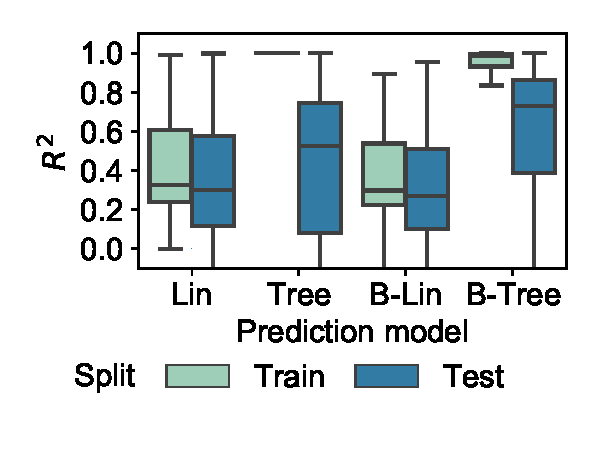
\includegraphics[width=\textwidth, trim=15 25 15 15, clip]{plots/syn-prediction-performance-all.pdf}
		\caption{All experimental runs.}
		\label{fig:syn:prediction-performance-all}
	\end{subfigure}
	\hfill
	\begin{subfigure}{0.48\textwidth}
		\centering
		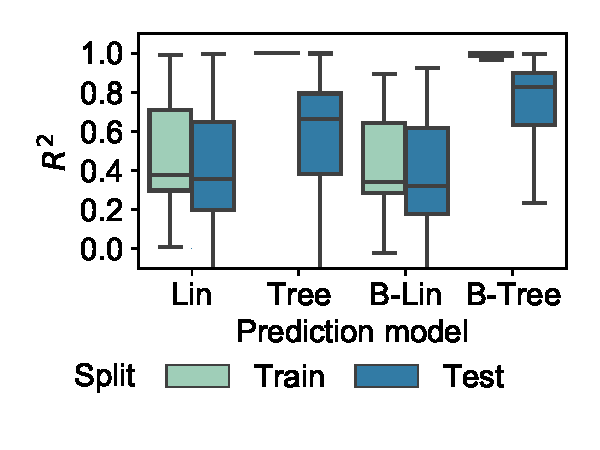
\includegraphics[width=\textwidth, trim=15 25 15 15, clip]{plots/syn-prediction-performance-unconstrained.pdf}
		\caption{Unconstrained experimental runs.}
		\label{fig:syn:prediction-performance-unconstrained}
	\end{subfigure}
	\caption{
		Distribution of prediction performance over datasets, cross-validation folds, and constraint-generation runs, by prediction model.
		Y-axes are truncated and outliers are removed to improve readability.
	}
	\label{fig:syn:prediction-performance}
\end{figure}

\subsection{Comparison of Prediction Models}
\label{sec:syn:evaluation:prediction}

Before studying the impact of constraints, we analyze prediction performance regarding the impact of the prediction model and dataset.
Figure~\ref{fig:syn:prediction-performance-all} shows a considerable variation in prediction performance for each model.
This plot aggregates all experimental runs, i.e., different datasets, cross-validation folds, constraint types, and constraint-generation repetitions.
However, Figure~\ref{fig:syn:prediction-performance-unconstrained} displays that there is still a considerable variation in prediction performance in the unconstrained~\ref{enum:syn:constraint-type:unconstrained} runs.
I.e., the datasets have a substantial impact on prediction performance.
We also see overfitting, i.e., the test-set performance is lower than the training-set performance, particularly for tree-based models.
In the following sections, we focus on test-set performance.
Further, we min-max normalize $R^2$ per dataset, cross-validation fold, and prediction model to focus on the relative impact of constraints, ignoring differences in dataset difficulty and model complexity.
Finally, we limit our analyses to two prediction models:
linear regression (\emph{Lin}), the simplest model we use, and gradient-boosted trees (\emph{B-Tree}), which yield the best average performance.

\begin{figure}[t]
	\centering
	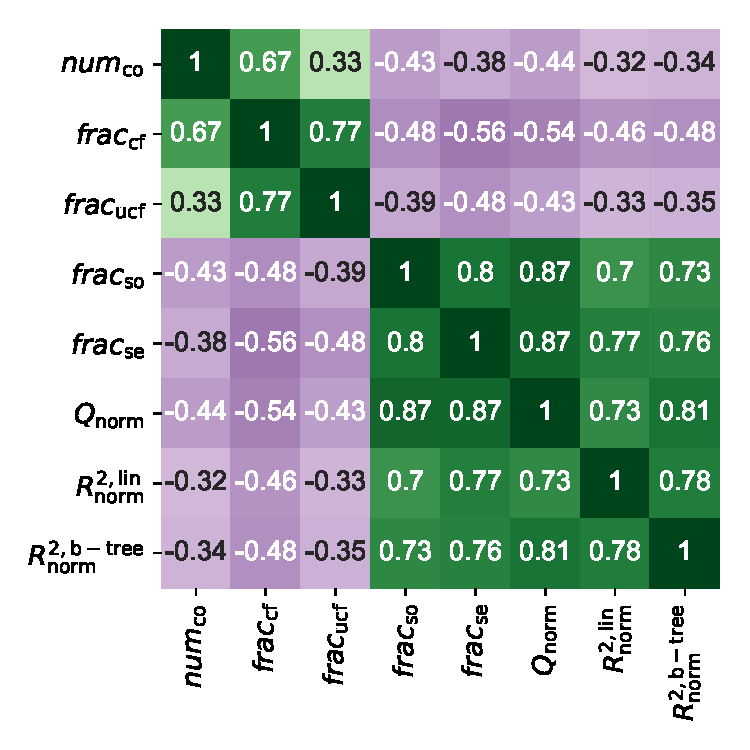
\includegraphics[width=0.66\textwidth, trim=10 10 10 10, clip]{plots/syn-evaluation-metrics-correlation.pdf}
	\caption{Spearman correlation between evaluation metrics, over datasets, cross-validation folds, and constraint-generation runs.}
	\label{fig:syn:evaluation-metrics-correlation}
\end{figure}

\begin{figure}[t]
	\centering
	\begin{subfigure}{0.48\textwidth}
		\centering
		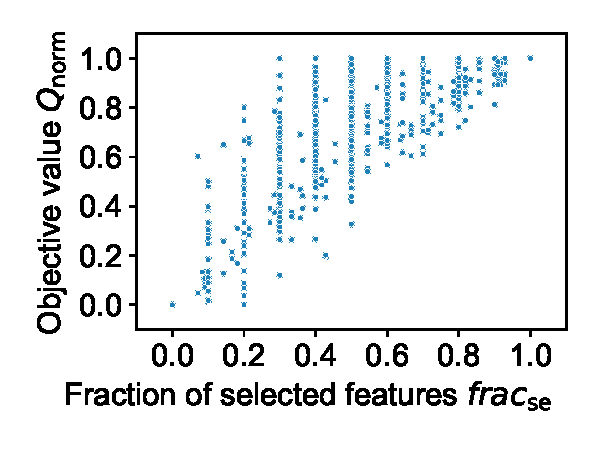
\includegraphics[width=\textwidth, trim=15 15 15 10, clip]{plots/syn-selected-vs-objective.pdf}
		\caption{Fraction of selected features.}
		\label{fig:syn:selected-vs-objective}
	\end{subfigure}
	\hfill
	\begin{subfigure}{0.48\textwidth}
		\centering
		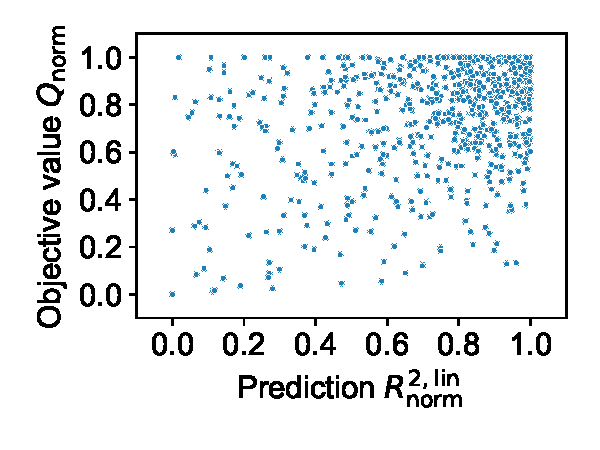
\includegraphics[width=\textwidth, trim=15 15 15 10, clip]{plots/syn-frac-linear-regression-r2-vs-objective.pdf}
		\caption{Test-set prediction performance of linear regression.}
		\label{fig:syn:frac-linear-regression-r2-vs-objective}
	\end{subfigure}
	\\
	\begin{subfigure}{0.48\textwidth}
		\centering
		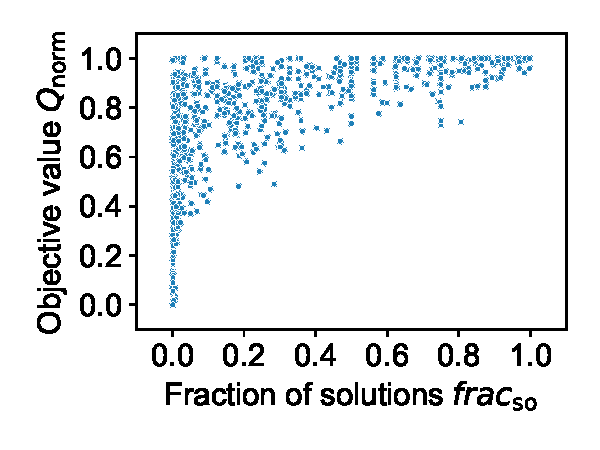
\includegraphics[width=\textwidth, trim=15 15 15 10, clip]{plots/syn-solutions-vs-objective.pdf}
		\caption{Fraction of solutions.}
		\label{fig:syn:solutions-vs-objective}
	\end{subfigure}
	\hfill
	\begin{subfigure}{0.48\textwidth}
		\centering
		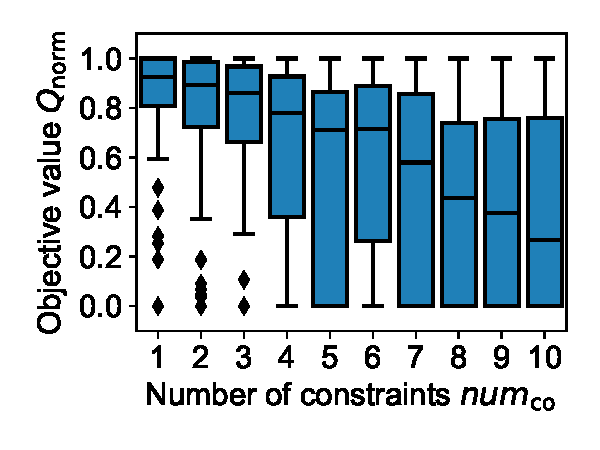
\includegraphics[width=\textwidth, trim=15 15 15 10, clip]{plots/syn-constraints-vs-objective.pdf}
		\caption{Number of constraints.}
		\label{fig:syn:constraints-vs-objective}
	\end{subfigure}
	\caption{
		Relationship of objective value~$Q_{\text{norm}}$ to other evaluation metrics.
		We have randomly sampled 1000 constraint-generation runs to keep the plot sizes and the time for rendering these plots reasonable.
	}
	\label{fig:syn:metrics-vs-metrics}
\end{figure}

\subsection{Relationship Between Evaluation Metrics}
\label{sec:syn:evaluation:metrics}

We study the relationships between evaluation metrics in two ways:
We analyze the correlation between metrics and also plot the metrics against each other.
For the correlation analysis, we take the values of each evaluation metric for all experimental runs and compute the Spearman rank correlation between these vectors.
The resulting correlation matrix (cf.~Figure~\ref{fig:syn:evaluation-metrics-correlation}) shows a strong positive correlation between the fraction of selected features~$\mathit{frac}_{\text{se}}$, the fraction of solutions~$\mathit{frac}_{\text{so}}$, the objective value~$Q_{\text{norm}}$, and the prediction performance~$R^{2}_{\text{norm}}$.
All pairwise correlations between these metrics are at least 0.7.

For a more detailed view, Figure~\ref{fig:syn:selected-vs-objective} shows a roughly linear relationship between the fraction of selected features~$\mathit{frac}_{\text{se}}$ and the objective value~$Q_{\text{norm}}$.
The linear objective function in our experiments (cf.~Section~\ref{sec:syn:experimental-design:objective}) makes this trend plausible.
However, the quality of the selected features and thus the objective value for a fixed feature-set size can still vary since different constraints may exclude different feature combinations.

Figure~\ref{fig:syn:frac-linear-regression-r2-vs-objective} shows that the objective value~$Q_{\text{norm}}$ and the prediction performance~$R^{2}_{\text{norm}}$ may lead to different assessments of feature-set quality.
The chosen objective function cannot describe interactions between features, as it only sums up the individual feature qualities.
This caveat is a general characteristic of univariate filter feature selection.
In contrast, prediction models evaluate a feature set as a whole.

Figure~\ref{fig:syn:solutions-vs-objective} shows that the relationship between the fraction of solutions~$\mathit{frac}_{\text{so}}$ and objective value~$Q_{\text{norm}}$ is non-linear.
Decreasing the fraction of valid feature sets tends to decrease the objective value.
However, it also matters which feature sets become invalid since the optimizer might find feature sets with a high objective value even in small search spaces, depending on the concrete constraints and the distribution of feature qualities.
In contrast, we have not observed any scenario with a large search space but a low objective value.

Coming back to the correlation matrix in Figure~\ref{fig:syn:evaluation-metrics-correlation},
there is a moderately negative correlation between the fraction of solutions~$\mathit{frac}_{\text{so}}$ on the one side and the number of constraints~$\mathit{num}_{\text{co}}$, fraction of constrained features~$\mathit{frac}_{\text{cf}}$, and fraction of unique constrained features~$\mathit{frac}_{\text{ucf}}$ on the other side.
This effect is expected since stronger constraint sets prune more solutions.
The correlation is only moderate, though, since the latter three metrics do not consider the constraint type.
E.g., for \emph{Group-NAND}~\ref{enum:syn:constraint-type:group-nand}, involving more features even makes the constraint weaker.
Further, the latter three metrics only show a moderately negative correlation to feature-set quality since they do not consider the individual feature qualities at all.
For example, Figure~\ref{fig:syn:constraints-vs-objective} shows the high variation in the relationship between the number of constraints~$\mathit{num}_{\text{co}}$ and the objective value~$Q_{\text{norm}}$.

\begin{figure}[t]
	\centering
	\begin{subfigure}{0.48\textwidth}
		\centering
		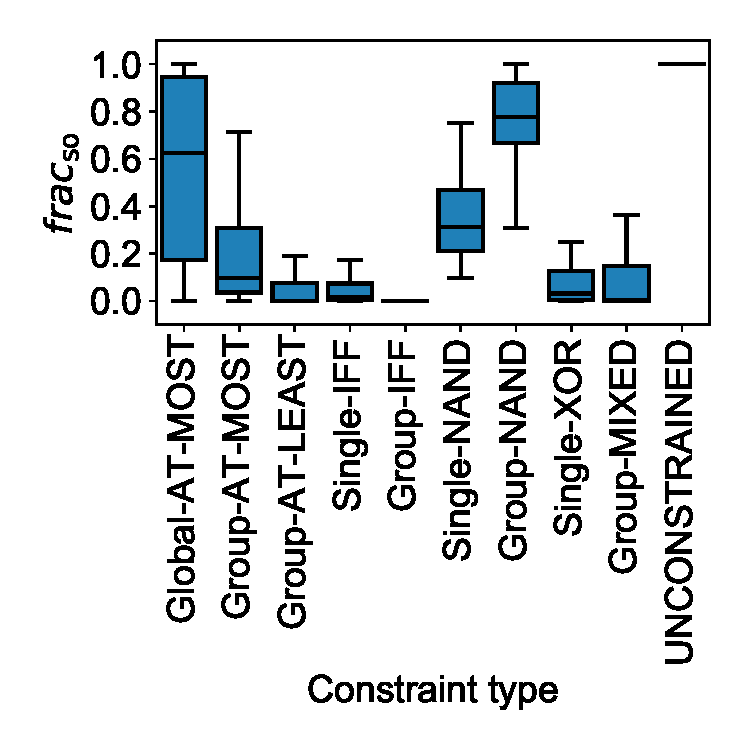
\includegraphics[width=\textwidth, trim=20 15 15 15, clip]{plots/syn-constraint-type-vs-solutions.pdf}
		\caption{Fraction of solutions.}
		\label{fig:syn:constraint-type-vs-solutions}
	\end{subfigure}
	\hfill
	\begin{subfigure}{0.48\textwidth}
		\centering
		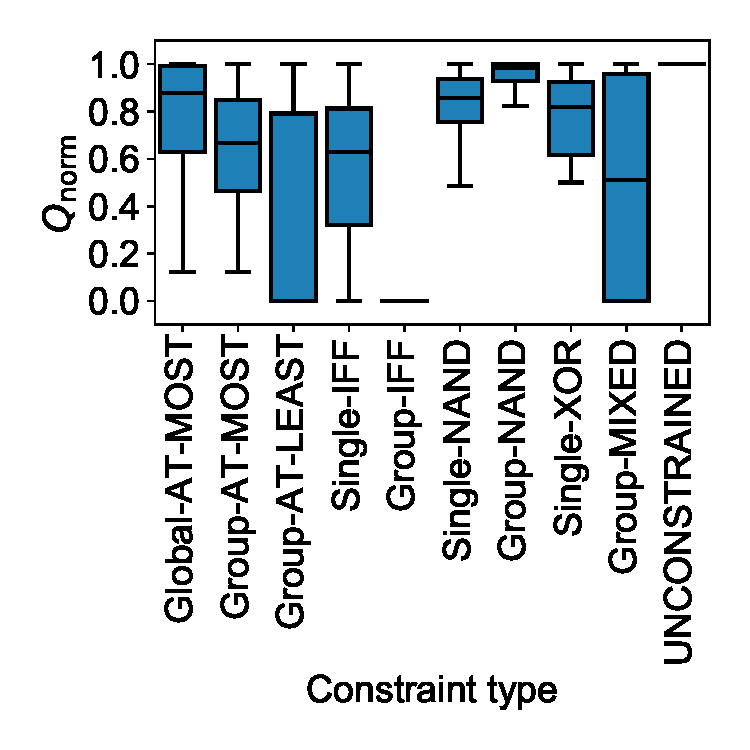
\includegraphics[width=\textwidth, trim=20 15 15 15, clip]{plots/syn-constraint-type-vs-objective.pdf}
		\caption{Objective value.}
		\label{fig:syn:constraint-type-vs-objective}
	\end{subfigure}
	\caption{
		Distribution of evaluation metrics over datasets, cross-validation folds, and constraint-generation runs, by constraint type.
		Outliers are removed to improve readability.
	}
	\label{fig:syn:constraint-type}
\end{figure}

\subsection{Impact of Constraint Types}
\label{sec:syn:evaluation:constraint-types}

Figure~\ref{fig:syn:constraint-type} shows how two evaluation metrics, i.e., fraction of solutions~$\mathit{frac}_{\text{so}}$ and objective value~$Q_{\text{norm}}$, vary between constraint types.
Normalized prediction performance exhibits similar trends as the objective value.
Overall, the impact of constraints strongly depends on the constraint type.
Without constraints, i.e., for the type \emph{UNCONSTRAINED}~\ref{enum:syn:constraint-type:unconstrained}, all feature sets are valid, and the objective value is maximal.
\emph{Global-AT-MOST}~\ref{enum:syn:constraint-type:global-at-most} has the largest inter-quartile range of the fraction of solutions (cf.~Figure~\ref{fig:syn:constraint-type-vs-solutions}).
This effect is expected since we systematically generate only one constraint of this type for each possible feature-set size, while the remaining constraint types employ up to 10 constraints (cf.~Algorithm~\ref{al:syn:constraint-generation}) and thereby typically limit the search space more.
Thus, \emph{GROUP-AT-MOST}~\ref{enum:syn:constraint-type:group-at-most} exhibits a smaller range and lower median of~$\mathit{frac}_{\text{so}}$ than \emph{Global-AT-MOST}~\ref{enum:syn:constraint-type:global-at-most}.
The type \emph{Group-MIXED}~\ref{enum:syn:constraint-type:group-mixed} shows the widest distribution of the objective value (cf.~Figure~\ref{fig:syn:constraint-type-vs-objective}) since it combines different other constraint types.
\emph{Single-NAND}~\ref{enum:syn:constraint-type:single-nand} and \emph{Group-NAND}~\ref{enum:syn:constraint-type:group-nand} exhibit only a small decrease in objective value since \emph{NAND} only excludes selecting all involved features simultaneously.
The more features are involved, the less restrictive the constraint becomes.
In contrast, \emph{IFF}~\ref{enum:syn:constraint-type:single-iff}~\ref{enum:syn:constraint-type:group-iff} constraints become stronger when applied to more features since they require either all of these features to be selected or none.
Further, remember that we combine \emph{IFF} with a \emph{Global-AT-MOST}~\ref{enum:syn:constraint-type:global-at-most} constraint to prevent the trivial outcome of selecting all features.
The more features are involved in \emph{IFF}s, the more difficult it becomes to satisfy the global cardinality constraint.
In the worst case, the set of selected features becomes empty, which is valid but has an objective value of zero.

\subsection{Summary}
\label{sec:syn:evaluation:summary}

We observed a relationship between the size of the search space~$\mathit{frac}_{\text{so}}$ and the feature-set quality, i.e., objective value~$Q_{\text{norm}}$ and prediction performance~$R^{2}_{\text{norm}}$.
Both the fraction of selected features $\mathit{frac}_{\text{se}}$ and the feature-set quality tended to decrease when constraints became stronger, i.e., pruned solutions.
However, the effect was non-linear, i.e., stronger constraints could still yield high feature-set quality.
In particular, there may be sweet spots, i.e., high-quality feature sets that adhere to the constraints.
While feature-set quality was strongly related to the fraction of solutions, the latter is costly to compute.
To a lesser extent, more coarse-grained metrics like the number of constraints~$\mathit{num}_{\text{co}}$ and the fraction of constrained features~$\mathit{frac}_{\text{cf}}$ were also related to feature-set quality.
Further, the distribution of evaluation metrics strongly depended on the constraint type.
Thus, it is difficult to make statements about the impact of constraints apart from some general trends. 
Finally, the optimization's objective value~$Q_{\text{norm}}$ and the prediction performance~$R^{2}_{\text{norm}}$ may yield different values for feature-set quality, particularly if the objective employs a simplified quality criterion like the linear function from Equation~\ref{eq:fs:univariate-filter}.

\chapter{Formulating Scientific Hypotheses as Constraints -- A Case Study}
\label{sec:ms}

\section{Overview}
\label{sec:ms:overview}

\paragraph{Scope}

In Chapter~\ref{sec:syn}, we formally introduced constrained feature selection and evaluated the impact of randomly generated constraints in a domain-independent manner.
We observed several general trends but also noted that the results depend on the constraint types.
In this chapter, we conduct a domain-specific case study in materials science.
The solver-based optimization approach for constrained feature selection remains the same as in Chapter~\ref{sec:syn}.
However, the goal and several other components of the current study's experimental design differ significantly from the previous study.
In particular, we involve users, and the constraints represent hypotheses and user preferences (cf.~Section~\ref{sec:introduction:research-gaps:integrating-domain-knowledge}).

\paragraph{Contributions}

Our contribution in this chapter is a case study to evaluate the impact of constraints for a concrete scenario.
We use a dataset from materials science with 135 features.
The dataset represents the microstructural evolution in a material specimen subjected to tensile loading.
The physical processes behind the data are complex and currently not fully understood.
Thus, we involve domain experts as users to formulate constraints.
We evaluate domain-specific hypotheses about the data by analyzing how the corresponding constraints affect feature selection, particularly feature-set quality and the composition of feature sets.
As in the study with generated constraints (cf.~Chapter~\ref{sec:syn}), we use univariate filter feature selection as the objective, formulate constraints with propositional logic and linear arithmetic, and find optimal feature sets with an SMT solver.
Section~\ref{sec:ms:evaluation:summary} summarizes key results.

\paragraph{Materials}

We publish all our code and experimental data online (cf.~Section~\ref{sec:introduction:materials}).

\paragraph{Prior works}

The content of this chapter bases on the following prior work:
%
\begin{itemize}
	\item \fullcite{bach2022empirical}
\end{itemize}

\paragraph{Chapter outline}

The remainder of this chapter is structured as follows:
Section~\ref{sec:ms:experimental-design} outlines our experimental design, and Section~\ref{sec:ms:evaluation} presents the experimental results.

\section{Experimental Design}
\label{sec:ms:experimental-design}

In this section, we introduce our experimental design for the case study in materials science.
First, we give a brief overview (cf.~Section~\ref{sec:ms:experimental-design:overview}).
Next, we present our scenario and dataset (cf.~Section~\ref{sec:ms:experimental-design:scenario}), objective function (cf.~Section~\ref{sec:ms:experimental-design:objective}), constraint types (cf.~Section~\ref{sec:ms:experimental-design:constraints}), evaluation metrics (cf.~Section~\ref{sec:ms:experimental-design:metrics}), and prediction models (cf.~Section~\ref{sec:ms:experimental-design:prediction}).
Finally, we briefly outline our implementation (cf.~Section~\ref{sec:ms:experimental-design:implementation}).

\subsection{Overview}
\label{sec:ms:experimental-design:overview}

In this case study, we evaluate constraints on one dataset from materials science.
In particular, we analyze twelve constraint types representing hypotheses from the domain and also add three domain-independent constraint types representing user preferences.
As in the study with generated constraints, we employ the objective of univariate filter feature selection.
We evaluate feature-set quality and the composition of the feature sets.

\subsection{Scenario and Dataset}
\label{sec:ms:experimental-design:scenario}

We collaborate with materials scientists who provide us with a dataset and act as domain experts for formulating constraints and interpreting results.
The general scenario of our study involves crystalline materials, such as most metals, on the micro-scale.
These materials incorporate defect structures, i.e., dislocations, within the regular crystal structure.
The line-like dislocations evolve over time and build complex 3D networks, which are mainly responsible for the permanent deformation of the material under load.
Understanding the network evolution is vital in characterizing the deformation behavior. 

The particular dataset in our study represents an aluminum specimen under tensile load~\cite{sudmanns2020data}.
Our domain experts created the dataset with numerical simulations using the method of discrete dislocation dynamics~\cite{weygand2001discrete}.
From a materials-science perspective, the research aims to study the evolution of properties characterizing the dislocation network.
An example of such a property is the slip system, i.e., the slip plane and slip direction in which a dislocation can move.
In face-centered cubic crystals, like our specimen, there are twelve slip systems.
Another example is the so-called Schmid factor.
It characterizes the slip plane and the slip direction that resolves the highest mechanical stress. 

\begin{table}[t]
	\centering
	\caption{
		Physical quantities and features in the materials-science dataset.
	}
	\begin{tabular}{llrrr}
		\toprule
		Base quantity & Symbol & Slip systems & Aggregates & Features \\
		\midrule
		edge\_resolved\_shear & $\sigma_\text{rss}^\text{edge}$ &            12 &           5 &        17 \\
		eps\_equiv & $\varepsilon_\text{eq}^\text{pl}$ &              0 &           0 &         1 \\
		eps\_xx & $\varepsilon_\text{xx}^\text{pl}$ &              0 &           0 &         1 \\
		eps\_xy & $\varepsilon_\text{xy}^\text{pl}$ &              0 &           0 &         1 \\
		eps\_xz & $\varepsilon_\text{xz}^\text{pl}$ &              0 &           0 &         1 \\
		eps\_yy & $\varepsilon_\text{yy}^\text{pl}$ &              0 &           0 &         1 \\
		eps\_yz & $\varepsilon_\text{yz}^\text{pl}$ &              0 &           0 &         1 \\
		eps\_zz & $\varepsilon_\text{zz}^\text{pl}$ &              0 &           0 &         1 \\
		free\_path\_per\_voxel & $\overline{l}_\text{norm}$ &              0 &           0 &         1 \\
		gamma & $\gamma$ &             12 &           5 &        17 \\
		gamma\_abs & $\gamma_\text{abs}$ &             12 &           5 &        17 \\
		kappa1 & $\kappa_\text{screw}$ &             12 &           5 &        17 \\
		kappa2 & $\kappa_\text{edge}$ &             12 &           5 &        17 \\
		mean\_free\_path & $\overline{l}$ &              0 &           0 &         1 \\
		n\_loops & $n_\text{loops}$ &              0 &           0 &         1 \\
		pos\_x & $x$ &              0 &           0 &         1 \\
		pos\_y & $y$ &              0 &           0 &         1 \\
		pos\_z & $z$ &              0 &           0 &         1 \\
		q & $q$ &             12 &           5 &        17 \\
		rho & $\rho$ &             12 &           5 &        17 \\
		step & -- &              0 &           0 &         1 \\
		time & $t$ &              0 &           0 &         1 \\
		vonMises & $\sigma_\text{vM}$ &              0 &           0 &         1 \\
		\bottomrule
	\end{tabular}
	\label{tab:ms:features}
\end{table}

Dislocation lines can react with each other in several ways.
Our prediction target is the density of dislocation line segments attached to so-called glissile reactions.
Table~\ref{tab:ms:features} gives an overview of the features in the dataset, which are other physical quantities of the system, like dislocation density, shear stress, etc.
Overall, the dataset consists of 14903 data objects and 135 features.
Each data object represents the state of the material specimen at a particular location and time step.
For predictions, we exclude the features for location, time, and simulation-step size, which leaves 130 features.
As Table~\ref{tab:ms:features} displays, some physical quantities correspond to one feature, while others yield 17 features.
In particular, some quantities in our dataset are measured separately for each of the twelve slip systems.
In this case, we also compute five aggregates, i.e., the minimum, maximum, median, sum, and standard deviation over the twelve slip systems.

\subsection{Objective Function and Optimization}
\label{sec:ms:experimental-design:objective}

As in the study with generated constraints (cf.~Section~\ref{sec:syn:experimental-design:objective}), we use the SMT solver \emph{Z3} \cite{bjorner2015nuz, deMoura2008z3} to optimize the univariate objective from Equation~\ref{eq:fs:univariate-filter}.
To instantiate the dependency measure~$q(\cdot)$, we take the absolute values of the Pearson correlation of each feature with the target variable, rather than the mutual information used in Chapter~\ref{sec:syn}.
In particular, preliminary experiments showed strong linear relationships in the data.
Also, the constraint types~\ref{enum:ms:constraint-type:inter-correlation} and~\ref{enum:ms:constraint-type:quality-filter}, which we introduce in the next section, assume that the dependency measure $q(\cdot)$ is bounded to $[0, 1]$, which mutual information violates.

\subsection{Constraints}
\label{sec:ms:experimental-design:constraints}

\paragraph{Overview}

This case study aims to evaluate the impact of constraints on feature selection in a concrete use case.
We did not identify firm domain knowledge suited for constraints.
However, we can still formulate constraints about hypothesized relationships between features.
We then evaluate how the resulting feature sets and feature-set quality change compared to an unconstrained selection.
Several outcomes are possible.
For example, the selected features may change, but the feature-set quality remains similar, indicating an alternative explanation.
Instead, feature-set quality may drop, indicating that the hypothesis behind the constraints is wrong.
By formulating different sets of constraints and evaluating them independently, one can also compare different hypotheses.

Besides domain-specific constraints representing the hypotheses, we also employ domain-independent constraints expressing preferences on the resulting feature sets.
As in our study with generated constraints (cf.~Chapter~\ref{sec:syn}), each constraint type may be formulated in multiple, logically equivalent ways.
In the following, we present one formulation each.

\paragraph{Domain-independent constraint types}

In preliminary experiments, we observed three phenomena that made it difficult for domain experts to interpret feature sets.
These phenomena were neither specific to our case study nor the domain in general.
We use three constraint types to alleviate these phenomena:
%
\begin{enumerate}[label=(I\arabic*), wide]
	\item\label{enum:ms:constraint-type:global-cardinality} \emph{Global-cardinality}:
	Larger feature sets may be harder to interpret for domain experts.
	Thus, we apply a global cardinality constraint, which is the same as~\ref{enum:syn:constraint-type:global-at-most} from the previous chapter.
	Here, we apply thresholds of $k \in \{5, 10\}$ features, so we can also compare how the feature-set quality changes from the smaller to the larger cardinality.
	%
	\begin{equation}
		\text{Global-cardinality}(\{s_1, \dots, s_n\}, k) =\\
		\sum_{j=1}^{n} s_j \leq k \text{, with } k \in \{5,10\}
		\label{eq:ms:constraint:global-cardinalty}
	\end{equation}
	%
	\item\label{enum:ms:constraint-type:inter-correlation} \emph{Inter-correlation}:
	Datasets may contain features strongly correlated with each other.
	Having such highly correlated features in the result may be undesirable, e.g., if they describe the same physical phenomenon, only measured or encoded differently.
	However, the objective function in Equation~\ref{eq:fs:univariate-filter} considers features independently, thus ignoring inter-feature correlation.
	Thus, we employ a correlation threshold:
	If a pair of features has an absolute Pearson correlation of at least $\tau = 0.8$, we select at most one of these features.
	The correlation values~$q(X_{\cdot{}j_1},X_{\cdot{}j_2})$ for each pair of features $j_1$,~$j_2$ can be precomputed and are therefore constants in the following formula, as is the user parameter~$\tau$.
	%
	\begin{multline}
		\text{Inter-correlation}(\{s_1, \dots, s_n\}, \tau) = \bigwedge_{\substack{(j_1, j_2) \in \{1, \dots, n\}^2 \\ j_1 \neq j_2}} \left( \left( q(X_{\cdot{}j_1},X_{\cdot{}j_2}) \geq \tau \right) \rightarrow \lnot (s_{j_1} \land s_{j_2}) \right)\\
		\text{with } \tau = 0.8
		\label{eq:ms:constraint:inter-correlation}
	\end{multline}
	%
	\item\label{enum:ms:constraint-type:quality-filter} \emph{Quality-filter}:
	Datasets may contain features with a quality close to zero.
	These features provide little value when being selected but may increase optimization time.
	Thus, it makes sense to remove such features manually before optimization or to add a respective constraint.
	We set a quality threshold of 0.2 and exclude features with a lower quality.
	The feature qualities~$q(X_{\cdot{}j},y)$ and the threshold $\tau$ are constants.
	%
	\begin{equation}
		\text{Quality-filter}(\{s_1, \dots, s_n\}, \tau) =\\
		\bigwedge_{j=1}^{n} \left( \left( q(X_{\cdot{}j},y) < \tau \right) \rightarrow \lnot s_j \right) \text{, with } \tau = 0.2
		\label{eq:ms:constraint:quality-filter}
	\end{equation}
	%
\end{enumerate}

\paragraph{Domain-specific constraint types}

The following constraint types express hypotheses:
%
\begin{enumerate}[label=(D\arabic*), wide]
	\item\label{enum:ms:constraint-type:schmid-group} \emph{Schmid-group}:
	For the crystal orientation of the considered specimen, the twelve slip systems can be divided into two non-overlapping groups based on the Schmid factor.
	Let $\mathbb{G}$ be this partitioning, i.e., a set of sets with $|\mathbb{G}| = 2$.
	We hypothesize that having features from at most one of these groups should suffice.
	Within the chosen group, an arbitrary number of features can be selected.
	To formalize this notion, let $P$ be the set of physical quantities measured for the twelve slip systems (cf.~Table~\ref{tab:ms:features}).
	Further, let the subscript $(p,g)$ identify a feature derived for a physical quantity $p$ and a slip system $g$.
	%
	\begin{equation}
		\text{Schmid-group}(\{s_1, \dots, s_n\}) = \sum_{G \in \mathbb{G}} \left( \bigvee_{p \in P,~g \in G} s_{(p,g)} \right) \leq 1
		\label{eq:ms:constraint:schmid-group}
	\end{equation}
	%
	\item\label{enum:ms:constraint-type:quantity-schmid-group} \emph{Quantity-Schmid-group}:
	The constraint type~\ref{enum:ms:constraint-type:schmid-group} goes over all physical quantities.
	Alternatively, one can choose between the two slip-system groups for each quantity independently.
	With such a constraint, we hypothesize that one slip-system group may be relevant for some quantities and the other group for other quantities.
	This constraint type makes feature selection more flexible, i.e., the hypothesis is less strict.
	%
	\begin{equation}
		\text{Quantity-Schmid-group}(\{s_1, \dots, s_n\}) = \bigwedge_{p \in P} \left( \sum_{G \in \mathbb{G}} \left( \bigvee_{g \in G} s_{(p,g)} \right) \leq 1 \right)
		\label{eq:ms:constraint:quantity-schmid-group}
	\end{equation}
	%
	\item\label{enum:ms:constraint-type:schmid-group-representative} \emph{Schmid-group-representative}:
	Using the grouping of~\ref{enum:ms:constraint-type:schmid-group}, one can also select at most one feature from each group instead of selecting features from at most one group.
	This constraint type corresponds to the situation where both groups are important, but it is sufficient to pick a representative feature in each group.
	%
	\begin{equation}
		\text{Schmid-group-representative}(\{s_1, \dots, s_n\}) = \bigwedge_{G \in \mathbb{G}} \left( \sum_{p \in P,~g \in G} s_{(p,g)} \leq 1 \right)
		\label{eq:ms:constraint:schmid-group-representative}
	\end{equation}
	%
	\item\label{enum:ms:constraint-type:quantity-schmid-group-representative} \emph{Quantity-Schmid-group-representative}:
	We merge the ideas of \ref{enum:ms:constraint-type:quantity-schmid-group} and \ref{enum:ms:constraint-type:schmid-group-representative}:
	For each quantity independently, select at most one feature per slip-system group.
	%
	\begin{equation}
		\text{Quantity-Schmid-group-representative}(\{s_1, \dots, s_n\}) = \bigwedge_{p \in P,~G \in \mathbb{G}} \left( \sum_{g \in G} s_{(p,g)} \leq 1 \right)
		\label{eq:ms:constraint:quantity-schmid-group-representative}
	\end{equation}
	%
	\item\label{enum:ms:constraint-type:plastic-strain-tensor} \emph{Plastic-strain-tensor}:
	Six features in our dataset describe the plastic strain tensor, corresponding to six different directions in space.
	These are the quantities starting with \emph{eps\_} in Table~\ref{tab:ms:features}, excluding \emph{eps\_quiv}.
	We hypothesize that selecting three of the six directions should be sufficient.
	To formalize this notion, let $T$ be a set of indices, identifying features that describe the plastic strain tensor.
	%
	\begin{equation}
		\text{Plastic-strain-tensor}(\{s_1, \dots, s_n\}) = \sum_{t \in T} s_t \leq 3
		\label{eq:ms:constraint:plastic-strain-tensor}
	\end{equation}
	%
	\item\label{enum:ms:constraint-type:dislocation-density} \emph{Dislocation-density}:
	In our dataset, several features describe dislocation density aggregated over all slip systems:
	the five standard aggregates of \emph{rho} as well as the quantities \emph{free\_path\_per\_voxel} and \emph{mean\_free\_path} (cf.~Table~\ref{tab:ms:features}).
	We hypothesize that selecting at most one such feature is sufficient.
	To formalize this notion, let $D$ be a set of indices, identifying features that describe dislocation density aggregated over all slip systems.
	%
	\begin{equation}
		\text{Dislocation-density}(\{s_1, \dots, s_n\}) = \sum_{d \in D} s_d \leq 1
		\label{eq:ms:dislocation-density}
	\end{equation}
	%
	\item\label{enum:ms:constraint-type:plastic-strain-rate} \emph{Plastic-strain-rate}:
	For the plastic strain rate, our dataset contains features originating from two different computation methods.
	These quantities are named \emph{gamma} and \emph{gamma\_abs} in Table~\ref{tab:ms:features}.
	We hypothesize that selecting features from at most one method should suffice.
	To formalize this notion, let $R_1$ and $R_2$ be sets of indices, identifying features originating from the two computation methods.
	%
	\begin{equation}
		\text{Plastic-strain-rate}(\{s_1, \dots, s_n\}) = \left( \bigvee_{r \in R_1} s_{r} \right) + \left( \bigvee_{r \in R_2} s_{r} \right) \leq 1
		\label{eq:ms:plastic-strain-rate}
	\end{equation}
	%
	\item\label{enum:ms:constraint-type:aggregate} \emph{Aggregate}:
	We have aggregated several physical quantities over the twelve slip systems (cf.~Table~\ref{tab:ms:features}).
	However, the five aggregate functions may be redundant to each other.
	Thus, we hypothesize that at most one kind of aggregate should suffice.
	To formalize this notion, let $P$ be the set of physical quantities measured for the twelve slip systems and let $A$ be the set of aggregate functions.
	Further, let subscript $(p,a)$ identify a feature derived for a physical quantity $p$ and an aggregate function $a$.
	%
	\begin{equation}
		\text{Aggregate}(\{s_1, \dots, s_n\}) = \sum_{a \in A} \left( \bigvee_{p \in P} s_{(p,a)} \right) \leq 1
		\label{eq:ms:constraint:aggregate}
	\end{equation}
	%
	\item\label{enum:ms:constraint-type:quantity-aggregate} \emph{Quantity-aggregate}:
	Constraint type~\ref{enum:ms:constraint-type:aggregate} can be refined to choose the aggregate function for each physical quantity independently.
	This new constraint type allows choosing different aggregate functions for different quantities.
	%
	\begin{equation}
		\text{Quantity-aggregate}(\{s_1, \dots, s_n\}) = \bigwedge_{p \in P} \left( \sum_{a \in A} s_{(p,a)} \leq 1 \right)
		\label{eq:ms:constraint:quantity-aggregate}
	\end{equation}
	%
	\item\label{enum:ms:constraint-type:aggregate-or-original} \emph{Aggregate-or-original}:
	Aggregates describe the same physical quantities as the features they aggregate.
	Thus, we hypothesize that selecting original features or aggregates for each quantity should suffice.
	To formalize this notion, let subscript $(p,l)$ identify a feature derived for a physical quantity $p$ and a slip system $l \in \{1, \dots, 12\}$.
	%
	\begin{equation}
		\text{Aggregate-or-original}(\{s_1, \dots, s_n\}) = \bigwedge_{p \in P} \left( \left( \bigvee_{a \in A} s_{(p,a)} \right) + \left( \bigvee_{l \in \{1, \dots, 12\}} s_{(p,l)} \right) \leq 1 \right)
		\label{eq:ms:aggregate-or-original}
	\end{equation}
	%
	\item\label{enum:ms:constraint-type:mixed} \emph{Mixed}:
	Various combinations of the previous constraint types above are possible, though some constraint types are redundant or compete with each other.
	For comparison, we consider the union of \ref{enum:ms:constraint-type:quantity-schmid-group-representative}, \ref{enum:ms:constraint-type:plastic-strain-tensor}, \ref{enum:ms:constraint-type:dislocation-density}, \ref{enum:ms:constraint-type:plastic-strain-rate}, \ref{enum:ms:constraint-type:quantity-aggregate}, and \ref{enum:ms:constraint-type:aggregate-or-original}.
	%
	\begin{equation}
		\begin{aligned}
			\text{Mixed}(\{s_1, \dots, s_n\}) &=~\text{Quantity-Schmid-group-representative}(\{s_1, \dots, s_n\}) \land \\
			& \text{Plastic-strain-tensor}(\{s_1, \dots, s_n\}) \land \\
			& \text{Dislocation-density}(\{s_1, \dots, s_n\}) \land \\
			& \text{Plastic-strain-rate}(\{s_1, \dots, s_n\}) \land \\
			& \text{Quantity-aggregate}(\{s_1, \dots, s_n\}) \land \\
			& \text{Aggregate-or-original}(\{s_1, \dots, s_n\})
		\end{aligned}
		\label{eq:ms:constraint:mixed}
	\end{equation}
	%
	\item\label{enum:ms:constraint-type:unconstrained} \emph{Unconstrained}:
	As a reference point, we evaluate the setting without domain-specific constraints.
	This definition is the same as~\ref{enum:syn:constraint-type:unconstrained} in the previous chapter.
	%
	\begin{equation}
		\text{Unconstrained}(\{s_1, \dots, s_n\}) = 1
		\label{eq:ms:constraint:unconstrained}
	\end{equation}
	%
\end{enumerate}

\paragraph{Combining domain-independent and domain-specific constraint types}

We create two sets of constraints from the domain-independent constraint types \ref{enum:ms:constraint-type:global-cardinality}, \ref{enum:ms:constraint-type:inter-correlation}, and \ref{enum:ms:constraint-type:quality-filter}.
Both sets involve all three types, but one uses the feature-set cardinality $k=5$, and the other $k=10$.
We combine each of these two constraint sets with each of the twelve domain-specific constraint types.
Thus, we get 24 constraint sets overall.
In the following evaluation, we mainly mention the names of the domain-specific constraint types, but the domain-independent constraint types are always active as well.

\subsection{Evaluation Metrics}
\label{sec:ms:experimental-design:metrics}

To evaluate our hypotheses expressed as constraints, we focus on selected features and feature-set quality, i.e., objective value and prediction performance.
In particular, we analyze how these outcomes differ between hypotheses.
Technically, we could use the complete set of evaluation metrics from the study with generated constraints (cf.~Section~\ref{sec:syn:experimental-design:metrics}).
However, we only have 24 experimental runs here, so statements on the relationship between evaluation metrics would be less generalizable.

\subsection{Prediction}
\label{sec:ms:experimental-design:prediction}

We use the same prediction models as in the study with generated constraints (cf.~Section~\ref{sec:syn:experimental-design:prediction}).
As our current dataset has a temporal dimension, we apply a time-based 80:20 holdout split instead of cross-validation,
i.e., all data objects in the training data are from earlier time steps than in the test data.
However, our predictions do not go into the future.
Instead, we predict the target variable from feature values at the same time step.

\subsection{Implementation and Execution}
\label{sec:ms:experimental-design:implementation}

As in the previous study (cf.~Section~\ref{sec:syn:experimental-design:implementation}), we implemented our experimental pipeline in Python~3.7, using \emph{scikit-learn}~\cite{pedregosa2011scikit-learn} and \emph{xgboost}~\cite{chen2016xgboost} for machine learning and the SMT solver \emph{Z3}~\cite{bjorner2015nuz, deMoura2008z3} for optimization.
All code is available online (cf.~Section~\ref{sec:introduction:materials}).
We organized the constrained-feature-selection functionality as a Python package.

Our experimental pipeline parallelizes over constraint types, while each of these experimental tasks runs single-threaded.
We ran the pipeline on a server with 128~GB RAM and an \emph{AMD EPYC 7551} CPU, having 32~physical cores and a base clock of 2.0~GHz.
With this hardware, the parallelized pipeline run took less than one hour.

\section{Evaluation}
\label{sec:ms:evaluation}

In this section, we evaluate our case study in materials science.
In particular, we analyze feature-set quality (cf.~Section~\ref{sec:ms:evaluation:quality}) and selected features (cf.~Section~\ref{sec:ms:evaluation:features}).
Finally, we summarize key findings (cf.~Section~\ref{sec:ms:evaluation:summary}).

\subsection{Feature-Set Quality}
\label{sec:ms:evaluation:quality}

\begin{figure}[t]
	\centering
	\begin{subfigure}{0.48\textwidth}
		\centering
		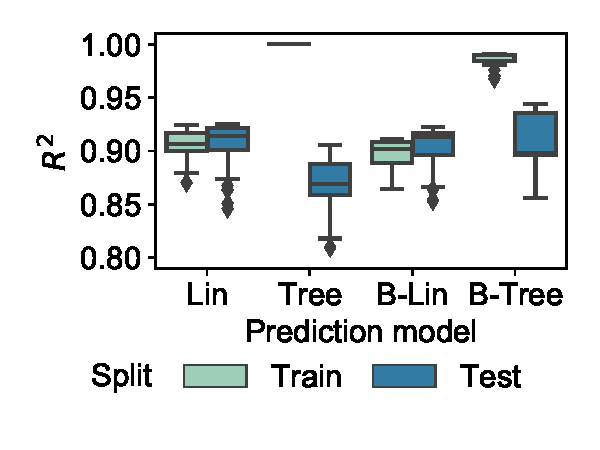
\includegraphics[width=\textwidth, trim=15 25 15 15, clip]{plots/ms-prediction-performance-split.pdf}
		\caption{All data, by split.}
		\label{fig:ms:prediction-performance-split}
	\end{subfigure}
	\hfill
	\begin{subfigure}{0.48\textwidth}
		\centering
		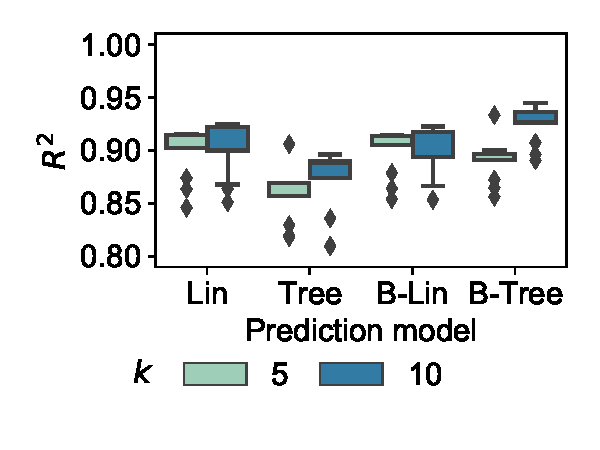
\includegraphics[width=\textwidth, trim=15 25 15 15, clip]{plots/ms-prediction-performance-cardinality.pdf}
		\caption{Only test data, by cardinality~$k$.}
		\label{fig:ms:prediction-performance-cardinality}
	\end{subfigure}
	\caption{Distribution of prediction performance over constraint types, by prediction model.}
	\label{fig:ms:prediction-performance}
\end{figure}

\paragraph{Prediction performance}

Figure~\ref{fig:ms:prediction-performance-split} shows the prediction performance over all 24 experimental runs.
All four prediction models perform well, even simple linear regression.
The twelve domain-specific constraint types cause some but not substantial variation in prediction performance.
Figure~\ref{fig:ms:prediction-performance-cardinality} shows that models with five features tend to perform only slightly worse than models with ten features.
I.e., one can make good predictions with a small set of features, which renders the scenario suitable for feature selection.

\paragraph{Objective value}

The objective value, i.e., summed univariate feature quality (cf.~Section~\ref{sec:ms:experimental-design:objective}), is also high and has a relatively low variance over constraint types.
In particular the objective value is in $[3.79, 4.04]$ for $k=5$ features and in $[6.45, 7.48]$ for $k=10$.
The theoretical upper bound on each feature's quality is~1.
In our dataset, the maximum feature quality is 0.92, and the average feature quality is 0.27.
Thus, the objective values achieved are considerably higher than the expected values, i.e.,
$0.27\cdot 5=1.35$ and $0.27 \cdot 10=2.7$.

The constraint type \emph{Mixed}~\ref{enum:ms:constraint-type:mixed} yields the lowest objective value for both cardinalities.
This type combines six other constraint types and thus restricts the search space more than the others.
Without this constraint type, the ranges of the objective value narrow down to $[3.92, 4.04]$ and $[7.03, 7.48]$.
I.e., our domain-specific constraint types have relatively little impact on the objective value.
In contrast, cardinality does have a noticeable impact, as can be expected from the linear objective.
Nevertheless, the size of the increase indicates that the sixth to tenth selected features still have relatively high quality.
This result should give way to alternative feature sets with similar quality, as we analyze later.

\paragraph{Comparing hypotheses}

As none of the analyzed constraint types significantly decrease feature-set quality, none of the underlying hypotheses seem to be invalidated.
Further, the modest variation of feature-set quality between hypotheses makes it challenging to draw conclusions regarding individual hypotheses.
A more detailed, domain-specific analysis of the hypotheses may be beneficial but is beyond the scope of this dissertation.

\subsection{Selected Features}
\label{sec:ms:evaluation:features}

\begin{figure}[t]
	\centering
	\begin{subfigure}{0.48\textwidth}
		\centering
		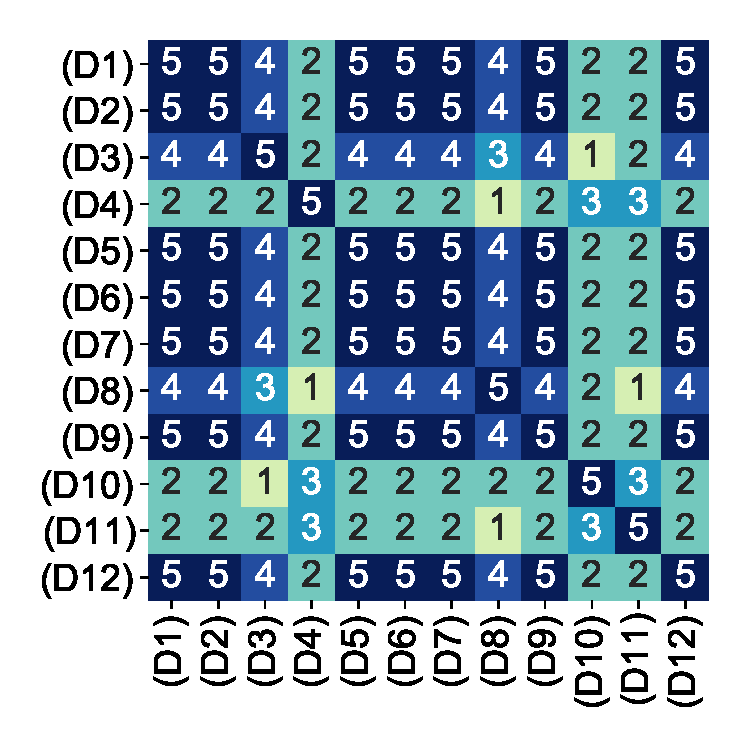
\includegraphics[width=\textwidth, trim=15 15 15 15, clip]{plots/ms-selected-similarity-card5.pdf}
		\caption{Cardinality $k=5$.}
		\label{fig:ms:selected-similarity-card5}
	\end{subfigure}
	\hfill
	\begin{subfigure}{0.48\textwidth}
		\centering
		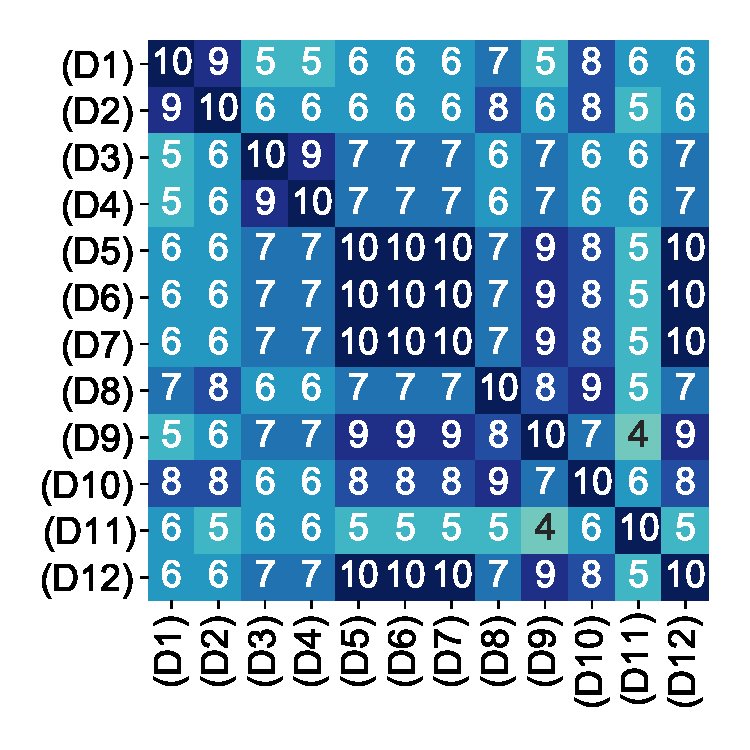
\includegraphics[width=\textwidth, trim=15 15 15 15, clip]{plots/ms-selected-similarity-card10.pdf}
		\caption{Cardinality $k=10$.}
		\label{fig:ms:selected-similarity-card10}
	\end{subfigure}
	\caption{Number of common features between resulting feature sets for different constraint types.}
	\label{fig:ms:selected-similarity}
\end{figure}

For all constraint types, the selected feature sets contain several dislocation-density-related features.
This observation is expected, as the target variable quantifies reactions of dislocations.
Figure~\ref{fig:ms:selected-similarity} shows how many selected features are the same when comparing results with different constraint types.
For $k=5$ (cf.~Figure~\ref{fig:ms:selected-similarity-card5}), several constraint types share more than half of their selected features.
In particular, six constraint types yield the same feature set as the reference case, i.e., \emph{Unconstrained}~\ref{enum:ms:constraint-type:unconstrained}.
We see two reasons for such `inactive' constraints.
First, the constraints may already be consistent with the unconstrained result even if they refer to its features.
For example, \emph{Unconstrained}~\ref{enum:ms:constraint-type:unconstrained} with $k=5$ only selects dislocation-density features from one slip-system group, so the constraint types \emph{Schmid-group}~\ref{enum:ms:constraint-type:schmid-group} and \emph{Quantity-Schmid-group}~\ref{enum:ms:constraint-type:quantity-schmid-group} are satisfied already.
Second, some constraint types may not affect any of the selected features in the reference case.
For example, \emph{Plastic-strain-rate}~\ref{enum:ms:constraint-type:plastic-strain-rate} and \emph{Plastic-strain-tensor}~\ref{enum:ms:constraint-type:plastic-strain-tensor} refer to physical quantities that have low quality in the prediction scenario. 
In future work, one might apply an iterative approach to avoid inactive constraints:
inspect the unconstrained result, formulate constraints, inspect the results, etc.

The picture becomes slightly more diverse for $k=10$ (cf.~Figure~\ref{fig:ms:selected-similarity-card10}).
Most constraint types still share at least half the selected features.
However, there are fewer cases where all features are the same since the reference case violates more constraint types now.
Still, as observed in the previous section, the feature-set quality is pretty similar between the constraint types.
For example, \emph{Mixed}~\ref{enum:ms:constraint-type:mixed} swaps 3/5 or 5/10 features compared to \emph{Unconstrained}~\ref{enum:ms:constraint-type:unconstrained}.
At the same time, the objective value only drops by 6.2\% or 13.8\%, which is a much smaller share.
This observation indicates that constraints may yield alternative feature sets that differ from the reference case but still have a similar quality.

\subsection{Summary}
\label{sec:ms:evaluation:summary}

We observed that our domain-specific constraint types had a relatively small impact on feature-set quality.
In other words, our analysis did not yield evidence against our hypotheses.
However, constraints resulted in features being replaced with alternatives of similar quality, motivating a principled approach for alternative feature selection (cf.~Chapter~\ref{sec:afs}).
Also, selecting only a few features sufficed to reach a high prediction performance.
Additionally, several constraint types were already satisfied in the solution of the unconstrained reference case.
Thus, we recommend an iterative approach of inspecting solutions and formulating new constraints instead of formulating all constraints upfront.

\chapter{Finding Alternative Feature Sets}
\label{sec:afs}

\section{Overview}
\label{sec:afs:overview}

\paragraph{Scope}

Our case study in Chapter~\ref{sec:ms} showed that differently composed feature sets of similar quality may exist.
However, these particular alternative feature sets were only a side-effect of employing different domain-specific constraints.
Nevertheless, obtaining such alternative solutions is generally desirable for users (cf.~Section~\ref{sec:introduction:research-gaps:finding-alternative-solutions}).
In this chapter, we formally introduce alternative feature selection in a domain-independent manner.
This new problem definition instantiates constrained feature selection (cf.~Chapter~\ref{sec:syn}) with particular constraint types.
Users can employ these predefined constraint types and configure them with user-friendly parameters.

\paragraph{Contributions}

Our contribution in this chapter is fivefold.

(1) We formalize alternative feature selection as an optimization problem, using 0-1 integer linear constraints to express alternative feature sets.
This approach is orthogonal to the feature-selection method so that users can choose the latter according to their needs.
Additionally, users may add further constraints on feature sets, e.g., to capture domain knowledge.
We let users control the search for alternatives with two parameters, i.e., the number of alternatives and a dissimilarity threshold.
For multiple alternatives, we consider sequential and simultaneous search.

(2) We discuss how to solve this optimization problem.
To that end, we describe how to integrate different categories of conventional feature-selection methods into the optimization problem's objective function.
In particular, we outline solver-based search methods for white-box and black-box optimization.

(3) We analyze the time complexity of the problem.
We show $\mathcal{NP}$-hardness, even for a simple notion of feature-set quality, i.e., univariate feature qualities.

(4) We propose heuristic search methods for univariate feature qualities.
We show that, under certain conditions, the optimization problem resides in the complexity class $\mathcal{APX}$, i.e., a constant-factor approximation exists.

(5) We conduct comprehensive experiments with 30 binary-classification datasets from the Penn Machine Learning Benchmarks (PMLB)~\cite{olson2017pmlb, romano2021pmlb} and five feature-selection methods.
We evaluate feature-set quality and runtime to investigate our search methods for alternatives and their user parameters.
Section~\ref{sec:afs:evaluation:summary} summarizes key results.

\paragraph{Materials}

We publish all our code and experimental data online (cf.~Section~\ref{sec:introduction:materials}).

\paragraph{Prior works}

The content of this chapter bases on the following prior works:
%
\begin{itemize}
	\item \fullcite{bach2023finding}
	\item \fullcite{bach2024alternative}
\end{itemize}

\paragraph{Chapter outline}

The remainder of this chapter is structured as follows:
Section~\ref{sec:afs:approach} describes and analyzes alternative feature selection.
Section~\ref{sec:afs:experimental-design} outlines our experimental design.
Section~\ref{sec:afs:evaluation} presents the corresponding experimental results.

\section{Alternative Feature Selection}
\label{sec:afs:approach}

In this section, we present the problem and approaches for alternative feature selection.
First, we define the overall structure of the optimization problem (cf.~Section~\ref{sec:afs:approach:problem}).
Second, we formalize alternatives via constraints (cf.~Section~\ref{sec:afs:approach:constraints}).
Third, we discuss objective functions for different feature-set quality measures and describe how to solve the resulting optimization problem (cf.~Section~\ref{sec:afs:approach:objectives}).
Fourth, we analyze the problem's time complexity (cf.~Section~\ref{sec:afs:approach:complexity}).
Fifth, we propose and analyze heuristic search methods for univariate feature qualities in the objective (cf.~Section~\ref{sec:afs:approach:univariate-heuristics}).

\subsection{Optimization Problem}
\label{sec:afs:approach:problem}

Alternative feature selection has two goals.
First, the quality of an alternative feature set should be high, as in conventional feature selection (cf.~Definition~\ref{def:fs:feature-selection}).
Second, an alternative feature set should differ from one or more other feature set(s).
There are several ways to combine these two goals in an optimization problem:

First, one can consider both goals as objectives, obtaining an unconstrained multi-objective problem.
Second, one can define constraints for both, feature-set quality and being alternative, searching for feasible solutions instead of optimizing.
Third, one can consider being alternative as objective and constrain feature-set quality, e.g., with a lower bound.
Fourth, one can treat feature-set quality as objective and enforce alternatives with constraints.

We pursue the last formulation, i.e., optimizing feature-set quality subject to being alternative.
This formulation is a special case of constrained feature selection (cf.~Definition~\ref{def:syn:constrained-feature-selection}) and keeps the original objective of feature selection.
Users need not set a threshold on feature-set quality but control how alternative the feature sets must be instead.
We obtain the following optimization problem for a single alternative feature set~$F_s$:

\begin{equation}
	\begin{aligned}
		\max_s &\quad Q(s,X,y) \\
		\text{subject to:} &\quad F_s~\text{being alternative}
	\end{aligned}
	\label{eq:afs:afs-general}
\end{equation}
%
In the following, we discuss different objective functions $Q(s,X,y)$ (cf.~Section~\ref{sec:afs:approach:objectives}) and suitable constraints for feature sets \emph{being alternative} (cf.~Section~\ref{sec:afs:approach:constraints}).
As in the previous chapter, we also typically limit the feature-set size $|F_s|$ to a user-defined value~$k \in \mathbb{N}$, which adds a further, simple constraint (cf.~Equation~\ref{eq:syn:cardinality}) to the optimization problem.

\subsection{Constraints -- Defining Alternatives}
\label{sec:afs:approach:constraints}

In this section, we formalize alternative feature sets.
First, we discuss the base case where an individual feature set is an alternative to another one (cf.~Section~\ref{sec:afs:approach:constraints:single}).
Second, we extend this notion to multiple alternatives, considering sequential and simultaneous search as two different problems (cf.~Section~\ref{sec:afs:approach:constraints:multiple}).
Our notion of alternatives is independent of the feature-selection method.
We provide two parameters, i.e., a dissimilarity threshold~$\tau$ and the number of alternatives~$a$, allowing users to control the search for alternatives.

\subsubsection{Single Alternative}
\label{sec:afs:approach:constraints:single}

We consider a feature set an alternative to another if it differs sufficiently.
Formally, we express this notion with a set-dissimilarity measure~\cite{choi2010survey, egghe2009new}.
Such measures typically assess set overlap and set sizes.
E.g., a well-known set-dissimilarity measure is the Jaccard distance, which is defined as follows for the (feature) sets $F'$ and $F''$:
%
\begin{equation}
	d_{\text{Jacc}}(F',F'') = 1 - \frac{|F' \cap F''|}{|F' \cup F''|} = 1 - \frac{|F' \cap F''|}{|F'| + |F''| - |F' \cap F''|}
	\label{eq:afs:jaccard}
\end{equation}
%
In this dissertation, we use a dissimilarity measure based on the Dice coefficient:
%
\begin{equation}
	d_{\text{Dice}}(F',F'') = 1 - \frac{2 \cdot |F' \cap F''|}{|F'| + |F''|}
	\label{eq:afs:dice}
\end{equation}
%
Generally, we only have mild assumptions on the set-dissimilarity measure~$d(\cdot)$.
Our subsequent definitions, examples, and propositions assume symmetry, i.e., $d(F',F'')=d(F'',F')$, normalization $d(\cdot) \in [0,1]$, and that $d(\cdot) = 1$ implies an empty intersection of the two sets.
In particular, $d(\cdot)$~does not need to be a metric but can also be a semi-metric~\cite{wilson1931semi} like~$d_{\text{Dice}}(\cdot)$.
In contrast to metrics, semi-metrics may violate the triangle inequality.

We leverage the set-dissimilarity measure~$d(\cdot)$ for the following definition:
%
\begin{definition}[Single alternative]
	Given a symmetric set-dissimilarity measure~$d(\cdot) \in [0, 1]$ with $d(\cdot) = 1$ implying no set overlap, and a dissimilarity threshold~$\tau \in [0, 1]$, a feature set $F'$ is an alternative to a feature set~$F''$ (and vice versa) if $d(F',F'') \geq \tau$.
	\label{def:afs:single-alternative}
\end{definition}
%
The threshold~$\tau$ controls how dissimilar alternative feature sets must be.
A larger~$\tau$ may reduce feature-set quality more, but the exact impact depends on the dataset and is unclear a priori.
Also, only users can decide which drop in feature-set quality is acceptable as a trade-off for obtaining alternatives.
Thus, we leave $\tau$ as a user parameter.
For dissimilarity measures $d(\cdot)$ with range $[0,1]$, like the Dice dissimilarity (cf.~Equation~\ref{eq:afs:dice}) or Jaccard distance (cf.~Equation~\ref{eq:afs:jaccard}), $\tau$~has a user-friendly interpretation:
$\tau=0$ allows identical feature sets, while $\tau=1$ implies zero overlap.
Users can adjust~$\tau$ to find an acceptable quality-dissimilarity trade-off, e.g., with a binary search over $\tau$'s range.

When implementing Definition~\ref{def:afs:single-alternative}, the following proposition gives way to using a broad range of solvers to tackle the related optimization problem:
%
\begin{proposition}[Linearity of constraints for alternatives]
	Using the Dice dissimilarity (cf.~Equation~\ref{eq:afs:dice}), alternative feature sets (cf.~Definition~\ref{def:afs:single-alternative}) can be expressed with 0-1 integer linear constraints.
	\label{prop:afs:linear-constraints}
\end{proposition}
%
\begin{proof}
	We re-arrange terms in the Dice dissimilarity (cf.~Equation~\ref{eq:afs:dice}) to eliminate the quotient of feature-set sizes:
	%
	\begin{equation}
		\begin{aligned}
			d_{\text{Dice}}(F',F'') &= & 1 - \frac{2 \cdot |F' \cap F''|}{|F'| + |F''|} &\geq \tau \\
			&\Leftrightarrow & |F' \cap F''| &\leq \frac{1 - \tau}{2} \cdot (|F'| + |F''|)
		\end{aligned}
		\label{eq:afs:dice-rearranged}
	\end{equation}
	%
	Next, we express the set sizes in terms of the feature-selection vector $s$:
	%
	\begin{equation}
		\begin{aligned}
			|F_s| =& \sum_{j=1}^n s_j \\
			|F_{s'} \cap F_{s''}| =& \sum_{j=1}^n s'_j \cdot s''_j
		\end{aligned}
		\label{eq:afs:feature-set-size}
	\end{equation}
	%
	Finally, we replace each product $s'_j \cdot s''_j$ with an auxiliary variable~$t_j$, bound by additional constraints, to linearize it~\cite{mosek2022modeling}:
	%
	\begin{equation}
		\begin{aligned}
			t_j \leq& s'_j \\
			t_j \leq& s''_j \\
			1 + t_j \geq& s'_j + s''_j \\
			t_j \in& \{0,1\}
		\end{aligned}
		\label{eq:afs:product-linear}
	\end{equation}
	%
	Combining Equations~\ref{eq:afs:dice-rearranged},~\ref{eq:afs:feature-set-size}, and~\ref{eq:afs:product-linear}, we obtain a set of constraints that only involve linear expressions of binary decision variables.
	In particular, there are only sum expressions and multiplications with constants but no products between variables.
	If one feature set is known, i.e., either $s'$ or $s''$ is fixed, Equation~\ref{eq:afs:feature-set-size} is already linear without Equation~\ref{eq:afs:product-linear}.
\end{proof}
%
Given a suitable objective function, which we discuss in Section~\ref{sec:afs:approach:objectives}, linear constraints allow using a broad range of solvers.
Alternatively, one could also encode these constraints into propositional logic (SAT)~\cite{ulrich2022selecting} to enable using another category of solvers.

If the set sizes $|F'|$ and $|F''|$ are constant, e.g., a user-defined~$k \in \mathbb{N}$, Equation~\ref{eq:afs:dice-rearranged} implies that the threshold~$\tau$ has a linear relationship to the maximum number of overlapping features~$|F' \cap F''|$.
This correspondence makes~$\tau$ easy to interpret, so we use the Dice dissimilarity in the following.
In contrast, the Jaccard distance leads to a non-linear relationship between $\tau$ and the overlap size (cf.~Definition~\ref{def:afs:single-alternative} with Equation~\ref{eq:afs:jaccard}):
%
\begin{equation}
	\begin{aligned}
		d_{\text{Jacc}}(F',F'') &= & 1 - \frac{|F' \cap F''|}{|F'| + |F''| - |F' \cap F''|} &\geq \tau \\
		&\Leftrightarrow & |F' \cap F''| &\leq \frac{1 - \tau}{2 - \tau} \cdot (|F'| + |F''|)
	\end{aligned}
	\label{eq:afs:jaccard-rearranged}
\end{equation}
%
Further, if $|F'| = |F''|$, as in our experiments, the Dice dissimilarity becomes identical to several other set-dissimilarity measures~\cite{egghe2009new}.
The parameter~$\tau$ then directly expresses which fraction of features in one set needs to differ from the other set and vice versa:
%
\begin{equation}
	d_{\text{Dice}}(F',F'') \geq \tau \Leftrightarrow |F' \cap F''| \leq (1 - \tau) \cdot |F'| = (1 - \tau) \cdot |F''|
	\label{eq:afs:dice-rearranged-equal-size}
\end{equation}
%
Thus, if users are uncertain how to choose $\tau$ and $|F'|$ is reasonably small, they can try out all values of $\tau \in \{l / |F'|\}$ with $l \in \{1, \dots, |F'|\}$.
In particular, these $|F'|$~unique values of $\tau$ suffice to produce all distinct solutions that one could obtain with an arbitrary $\tau \in (0,1]$.

\subsubsection{Multiple Alternatives}
\label{sec:afs:approach:constraints:multiple}

If users desire multiple alternative feature sets rather than only one, we can determine these alternatives sequentially or simultaneously.
The number of alternatives~$a \in \mathbb{N}_0$ is a parameter to be set by the user.
The overall number of feature sets is $a + 1$ since we deem one feature set the \emph{original} one.
Table~\ref{tab:afs:seq-sim-comparison} shows the sizes of the two search problems.

\begin{table}[t]
	\centering
	\caption{Number of variables and constraints for $a$~alternatives ($a + 1$~feature sets overall) and $n$ features.}
	\renewcommand*{\arraystretch}{1.3}
	\begin{tabular}{lccc}
		\toprule
		& \multicolumn{2}{c}{Sequential search} & \multirow{2}{*}{Simultaneous search} \\
		\cmidrule(lr){2-3}
		& $l$-th Alternative & Summed & \\
		\midrule
		Decision variables~$s$ & $n$ & $ (a+1) \cdot n$ & $(a+1) \cdot n$ \\
		Linearization variables~$t$ & $0$ & $0$ & $\frac{a \cdot (a+1) \cdot n}{2}$ \\
		Alternative constraints & $l$ & $\frac{a \cdot (a+1)}{2}$ & $\frac{a \cdot (a+1)}{2}$ \\
		Linearization constraints & $0$ & $0$ & $\frac{3 \cdot a \cdot (a+1) \cdot n}{2}$ \\
		\bottomrule
	\end{tabular}
	\label{tab:afs:seq-sim-comparison}
\end{table}

\paragraph{Sequential-search problem}

In the sequential-search problem, users obtain several alternatives iteratively, with one feature set per iteration.
We constrain this new set to be an alternative to all previously found ones, which are given in a set~$\mathbb{F}$:
%
\begin{definition}[Sequential alternative]
	A feature set~$F''$ is an alternative to a set of feature sets~$\mathbb{F}$ (and vice versa) if $F''$ is a single alternative (cf.~Definition~\ref{def:afs:single-alternative}) to each $F' \in \mathbb{F}$.
	\label{def:afs:sequential-alternative}
\end{definition}
%
One could also think of less strict constraints, e.g., only bounding the average dissimilarity to all previously found feature sets.
However, definitions like the latter may allow some feature sets to overlap heavily or even be identical if others are very dissimilar.
Thus, we require pairwise dissimilarity in Definition~\ref{def:afs:sequential-alternative}.
Combining Equation~\ref{eq:afs:afs-general} with Definition~\ref{def:afs:sequential-alternative}, we obtain the following optimization problem for each iteration of the search:
%
\begin{equation}
	\begin{aligned}
		\max_s &\quad Q(s,X,y) \\
		\text{subject to:} &\quad \forall F' \in \mathbb{F}:~d(F_s,F') \geq \tau
	\end{aligned}
	\label{eq:afs:afs-sequential}
\end{equation}
%
The full textual problem definition corresponding to Equation~\ref{eq:afs:afs-sequential} is the following:
%
\begin{definition}[Sequential-search problem for one alternative feature set]
	Given
	\begin{itemize}[noitemsep]
		\item a dataset~$X \in \mathbb{R}^{m \times n}$ with prediction target~$y \in Y^m$,
		\item a set~$\mathbb{F}$ of existing feature sets for~$X$,
		\item a symmetric set-dissimilarity measure~$d(\cdot) \in [0,1]$ with $d(\cdot) = 1 \rightarrow$ no set overlap,
		\item and a dissimilarity threshold~$\tau \in [0,1]$,
	\end{itemize}
	sequential search for one alternative feature set is the problem of making feature-selection decisions~$s \in \{0,1\}^n$ that maximize a given notion of feature-set quality~$Q(s,X,y)$ while making the corresponding feature set~$F_s$ a sequential alternative to~$\mathbb{F}$ (cf.~Definition~\ref{def:afs:sequential-alternative}).
	\label{def:afs:alternative-feature-selection-sequential}
\end{definition}
%
We solve this optimization problem repeatedly, thereby optimizing only one feature set's quality at once.
$\mathbb{F} = \emptyset$ in the first iteration yields the \emph{original} feature set, i.e., the best unconstrained feature set.
Each alternative enlarges~$\mathbb{F}$ and adds one constraint, but the number of decision variables remains the same.
Further, we do not need to introduce linearization variables (cf.~Equation~\ref{eq:afs:product-linear}) since all feature sets except one are fixed.
Thus, the runtime of a solver-based sequential search should scale well with the number of alternatives.
Additional runtime gains may arise if the solver keeps a state between iterations and can warm-start.
Further, users do not need to define the number of alternatives a priori but can stop after each iteration once the feature-set quality is too low.
As a caveat, the stepwise optimization may yield alternatives with significantly different quality.

\paragraph{Simultaneous-search problem}

In the simultaneous-search problem, users obtain multiple alternatives at once, so they need to decide on the number of alternatives~$a$ beforehand.
We use pairwise dissimilarity constraints for alternatives again:
%
\begin{definition}[Simultaneous alternatives]
	A set of feature sets~$\mathbb{F}$ contains simultaneous alternatives if each feature set~$F' \in \mathbb{F}$ is a single alternative (cf.~Definition~\ref{def:afs:single-alternative}) to each other feature set~$F'' \in \mathbb{F}$ with $F' \neq F''$.
	\label{def:afs:simultaneous-alternative}
\end{definition}
%
Combining Equation~\ref{eq:afs:afs-general} with Definition~\ref{def:afs:simultaneous-alternative}, we obtain the following optimization problem for $a+1$ feature sets, i.e., including the original feature set:
%
\begin{equation}
	\begin{aligned}
		\max_{s^{(0)}, \dots, s^{(a)}} &\quad \operatorname*{agg}_{l \in \{0, \dots, a\}} Q(s^{(l)},X,y) \\
		\text{subject to:} &\quad \forall l_1, l_2 \in \{0, \dots, a\},~l_1 \neq l_2:~d(F_{s^{(l_1)}},F_{s^{(l_2)}}) \geq \tau
	\end{aligned}
	\label{eq:afs:afs-simultaneous}
\end{equation}
%
The full textual problem definition corresponding to Equation~\ref{eq:afs:afs-simultaneous} is the following:
%
\begin{definition}[Simultaneous-search problem for alternative feature sets]
	Given
	\begin{itemize}[noitemsep]
		\item a dataset~$X \in \mathbb{R}^{m \times n}$ with prediction target~$y \in Y^m$,
		\item the number of alternatives~$a \in \mathbb{N}_0$,
		\item an aggregation operator $\text{agg}(\cdot): \mathbb{R}^{a+1} \to \mathbb{R}$ for feature-set qualities,
		\item a symmetric set-dissimilarity measure~$d(\cdot) \in [0,1]$ with $d(\cdot) = 1 \rightarrow$ no set overlap,
		\item and a dissimilarity threshold~$\tau \in [0,1]$,
	\end{itemize}
	simultaneous search for alternative feature sets is the problem of making feature-selection decisions~$s^{(l)} \in \{0,1\}^n$ for $l \in \{0, \dots, a\}$ that maximize a given notion of feature-set quality~$Q(s,X,y)$ aggregated over the alternatives with $\operatorname*{agg}_{l \in \{0, \dots, a\}} Q(s^{(l)},X,y)$ while making the corresponding feature sets $\mathbb{F} = \{F_{s^{(0)}}, \dots, F_{s^{(a)}}\}$ simultaneous alternatives (cf.~Definition~\ref{def:afs:simultaneous-alternative}).
	\label{def:afs:alternative-feature-selection-simultaneous}
\end{definition}
%
In contrast to the sequential case (cf.~Definition~\ref{def:afs:alternative-feature-selection-sequential}), the problem requires $a+1$ instead of one decision vector~$s$ of length~$n$, and a modified objective function.
The operator~$\text{agg}(\cdot)$ defines how to aggregate the feature-set qualities of the alternatives, which we discuss later.
Runtime-wise, exact simultaneous search should scale worse with the number of alternatives than exact sequential search, as it tackles one large optimization problem instead of multiple smaller ones.
Besides requiring more decision variables, we need to introduce an auxiliary variable for each feature and pair of alternatives if we want to obtain linear constraints (cf.~Equation~\ref{eq:afs:product-linear} and Table~\ref{tab:afs:seq-sim-comparison}).
Quality-wise, simultaneous search may have an advantage over sequential search due to optimizing alternatives globally rather than greedily.
Also, the quality can be more evenly distributed over the alternatives, as opposed to the dropping quality over the course of the sequential procedure.
As a downside, there are no intermediate steps where users could interrupt the search.

\paragraph{Sum-aggregation}

One straightforward way to aggregate the qualities of feature sets in the simultaneous-search objective is to sum them up, which we call \emph{sum-aggregation}:
%
\begin{equation}
	\max_{s^{(0)}, \dots, s^{(a)}} \sum_{l=0}^a Q(s^{(l)},X,y)
	\label{eq:afs:afs-simultaneous-sum-objective}
\end{equation}
%
While this objective fosters a high average feature-set quality, it does not guarantee that the alternatives have similar quality:
%
\begin{example}[Sum-aggregation]
	Consider $n=6$~features with univariate feature qualities (cf.~Equation~\ref{eq:fs:univariate-filter}) $q = (9,8,7,3,2,1)$, feature-set size~$k=3$, number of alternatives~$a=2$, the Dice dissimilarity (cf.~Equation~\ref{eq:afs:dice}) as~$d(\cdot)$, and dissimilarity threshold~$\tau = 0.5$, which permits an overlap of one feature between sets here (cf.~Equation~\ref{eq:afs:dice-rearranged-equal-size}).
	Exact sequential search (cf.~Definition~\ref{def:afs:alternative-feature-selection-sequential}) yields the selection $s^{(0)} = (1,1,1,0,0,0)$, $s^{(1)} = (1,0,0,1,1,0)$, and $s^{(2)} = (0,1,0,1,0,1)$, with a summed quality of $\,24+14+12=50$.
	One possible exact simultaneous-search (cf.~Definition~\ref{def:afs:alternative-feature-selection-simultaneous}) solution consists of the feature sets $s^{(0)} = (1,1,0,1,0,0)$, $s^{(1)} = (1,0,1,0,1,0)$, and $s^{(2)} = (0,1,1,0,0,1)$, with a summed quality of $\,20+18+16=54$.
	Another possible exact simultaneous-search solution is $s^{(0)} = (1,1,0,0,0,1)$, $s^{(1)} = (1,0,1,0,1,0)$, and $s^{(2)} = (0,1,1,1,0,0)$, with a summed quality of $\,18+18+18=54$.
	\label{ex:afs:sum-aggregation}
\end{example}
%
This example yields several insights.
First, exact sequential search yields worse quality than exact simultaneous search here, i.e., 50 vs.~54.
Second, the feature-set qualities of the sequential solution, i.e., 24, 14, and~12, differ significantly.
Third, an exact simultaneous search can admit multiple solutions whose feature-set quality is differently balanced.
I.e., the solution with feature-set qualities 18, 18, and~18 is more balanced than the one with 20, 18, and~16.
However, both solutions are equally optimal for sum-aggregation.

\paragraph{Min-aggregation}

To actively foster balanced feature-set qualities in simultaneous search, we propose \emph{min-aggregation} in the objective:
%
\begin{equation}
	\max_{s^{(0)}, \dots, s^{(a)}} \min_{l \in \{0, \dots, a\}} Q(s^{(l)},X,y) \\
	\label{eq:afs:afs-simultaneous-min-objective}
\end{equation}
%
This formulation maximizes the quality of the worst alternative.
Thereby, it incentivizes all alternatives to have high quality and implicitly balances their quality.
In the terminology of social choice theory, it uses an egalitarian rule instead of a utilitarian one~\cite{myerson1981utilitarianism}.

Optimizing with either sum-aggregation or min-aggregation does not necessarily optimize the other.
Example~\ref{ex:afs:sum-aggregation} already showed a solution optimizing sum-aggregation but not min-aggregation.
In the following, we demonstrate the other direction:
%
\begin{example}[Min-aggregation]
	Consider $n=6$~features with univariate feature qualities (cf.~Equation~\ref{eq:fs:univariate-filter}) $q = (11,10,6,5,4,1)$, feature-set size~$k=3$, number of alternatives~$a=1$, the Dice dissimilarity (cf.~Equation~\ref{eq:afs:dice}) as~$d(\cdot)$, and dissimilarity threshold~$\tau = 0.5$, which permits an overlap of one feature between sets here (cf.~Equation~\ref{eq:afs:dice-rearranged-equal-size}).
	One simultaneous-search (cf.~Definition~\ref{def:afs:alternative-feature-selection-simultaneous}) solution with min-aggregation (cf.~Equation~\ref{eq:afs:afs-simultaneous-min-objective}) is $s^{(0)} = (1,1,0,0,1,0)$ and $s^{(1)} = (1,0,1,1,0,0)$, with a summed quality of $\,25+22=47$.
	Another solution is $s^{(0)} = (1,1,0,0,0,1)$ and $s^{(1)} = (1,0,1,1,0,0)$, with a summed quality of $\,22+22=44$.
	\label{ex:afs:min-aggregation}
\end{example}
%
While both solutions have the same minimum feature-set quality, only the first solution optimizes sum-aggregation.
In particular, min-aggregation permits reducing the quality of feature sets as long as the latter remains above the minimum quality of all sets.

From the technical perspective, Equation~\ref{eq:afs:afs-simultaneous-min-objective} has the disadvantage of being non-linear regarding the decision variables $s^{(0)}, \dots, s^{(a)}$.
However, we can linearize it with an auxiliary variable~$Q_{\text{min}}$ and one constraint per feature set:
%
\begin{equation}
	\begin{aligned}
		\max_{s^{(0)}, \dots, s^{(a)}} &\quad &Q_{\text{min}} & \\
		\text{subject to:} &\quad \forall l \in \{0, \dots, a\}: &Q_{\text{min}} &\leq Q(s^{(l)},X,y) \\
		&\quad & Q_{\text{min}} &\in \mathbb{R}
	\end{aligned}
	\label{eq:afs:afs-simultaneous-min-objective-linear}
\end{equation}
%
As we maximize~$Q_{\text{min}}$, this variable will implicitly assume the actual minimum value of~$Q(s^{(l)},X,y)$ with equality since the solution would not be optimal otherwise.
This situation relieves us from introducing further auxiliary variables that are usually necessary when linearizing maximum or minimum expressions~\cite{mosek2022modeling}.

\paragraph{Further approaches for balancing quality}

Min-aggregation provides no control or guarantee of how much the feature-set qualities will actually differ between alternatives.
One can alleviate this issue by adapting the objective or constraints.
First, related work on \textsc{Multi-Way Number Partitioning} also uses other objectives for balancing~\cite{korf2010objective, lawrinenko2017identical}.
E.g., one could minimize the difference between maximum and minimum feature-set quality.
Second, one could use sum-aggregation but constrain the minimum or maximum quality of sets or the difference between them.
However, such constraint-based approaches introduce one or several quality-threshold parameters that are difficult to determine a priori.
Third, one could treat balancing qualities as another objective besides maximizing the summed quality.
One can then optimize two objectives simultaneously, filtering results for Pareto-optimal solutions or optimizing a weighted combination of the two objectives.
In both cases, users may need to define an acceptable trade-off between the objectives.

\subsection{Objective Functions -- Finding Alternatives}
\label{sec:afs:approach:objectives}

In this section, we discuss how to find alternative feature sets.
In particular, we describe how to address the different categories of feature-set quality measures from Section~\ref{sec:fundamentals:feature-selection:methods} in the optimization problem from Section~\ref{sec:afs:approach:problem}.
We consider white-box (cf.~Section~\ref{sec:afs:approach:objectives:white-box}), black-box (cf.~Section~\ref{sec:afs:approach:objectives:black-box}), and embedded approaches (cf.~Section~\ref{sec:afs:approach:objectives:embedding}).

\subsubsection{White-Box Optimization}
\label{sec:afs:approach:objectives:white-box}

If the structure of the alternative-feature-selection problem is sufficiently simple, one can employ a solver for white-box optimization (cf.~Section~\ref{sec:syn:approach:optimization}).
We already showed that our notion of alternative feature sets results in 0-1 integer linear constraints (cf.~Proposition~\ref{prop:afs:linear-constraints}).
We now discuss several feature-selection methods with objectives, i.e., feature-set quality functions~$Q(s,X,y)$, that admit formulating a 0-1 integer linear problem.

\paragraph{Univariate filter feature selection}

For univariate filter feature selection (cf.~Equation~\ref{eq:fs:univariate-filter}), the objective function is linear by default.
Due to its simplicity, this objective admits various formalizations and search methods.
Appendix~\ref{sec:appendix:afs:univariate-complete-optimization-problem} specifies the complete 0-1 integer linear optimization problem, including the constraints for alternatives.
Section~\ref{sec:afs:approach:univariate-heuristics} proposes heuristic search methods.
As another encoding for solver-based search, one could formulate a weighted \textsc{Max One} problem~\cite{khanna1997complete}, i.e., a special type of \textsc{MaxSAT} problem~\cite{bacchus2021maximum, li2021maxsat}.
In particular, Equation~\ref{eq:fs:univariate-filter} is a sum of weighted binary variables, and a cardinality encoding~\cite{sinz2005towards} can turn the constraints for alternatives into SAT formulas.

Further, the monotonicity of the univariate objective enables speeding up arbitrary search methods if the user-defined feature-set sizes~$k$ and the number of alternatives~$a$ are small.
In particular, replacing one selected feature with another feature of lower quality cannot increase the objective value.
Sum-aggregation (cf.~Equation~\ref{eq:afs:afs-simultaneous-sum-objective}) and min-aggregation (cf.~Equation~\ref{eq:afs:afs-simultaneous-min-objective}) for the simultaneous-search problem are monotonic as well.
Thus, assuming $(a + 1) \cdot k < n$, it suffices to use the $(a + 1) \cdot k$ highest feature qualities when searching for an optimal solution with $a + 1$ feature sets.
As the remaining feature qualities cannot improve the objective, one can drop them before optimization.
We call this step \emph{pre-selection}.
While there may also be optimal solutions using the dropped features, their objective value cannot be higher.
Such solutions may arise in case of multiple identical qualities or for min-aggregation.
Also, the optimal solution may not contain all pre-selected features, i.e., pre-selection over-approximates the set of finally selected features.

\paragraph{Post-hoc feature importance}

Technically, one can also insert the values of post-hoc feature-importance scores (cf.~Section~\ref{sec:fundamentals:feature-selection:methods:importance}) as univariate feature qualities~$q(X_{\cdot{}j},y)$ into Equation~\ref{eq:fs:univariate-filter}.
However, such post-hoc importance scores typically evaluate the quality of each feature in the presence of the dataset's other features, i.e., the scores are not truly univariate.
Thus, treating pre-computed post-hoc importance scores as univariate feature qualities in the optimization objective is a simplification and may not faithfully represent the actual feature qualities in a particular subset of selected features~\cite{fryer2021shapley}.

\paragraph{FCBF}

While the original FCBF (cf.~Section~\ref{sec:fundamentals:feature-selection:methods:filter}) is an algorithm, we formulate a constrained optimization problem to enable a solver-based optimization for alternatives:
%
\begin{equation}
	\begin{aligned}
		\max_s &\quad Q_{\text{FCBF}}(s,X,y) = \sum_{j=1}^{n} q(X_{\cdot{}j},y) \cdot s_j \\
		\text{subject to:} &\quad \forall j_1, j_2 \in \{1, \dots, n\},~j_1 \neq j_2,~(*): s_{j_1} + s_{j_2} \leq 1 \\
		\text{with } (*) \text{:} &\quad q(X_{\cdot{}j_1},y) \leq q(X_{\cdot{}j_2}, X_{\cdot{}j_1}) \\
	\end{aligned}
	\label{eq:afs:fcbf}
\end{equation}
%
We drop the original FCBF's threshold on feature-target correlation and maximize the latter instead, as in the univariate-filter case.
Further, we keep FCBF's constraints on feature-feature correlation.
In particular, we prevent the simultaneous selection of two features if the correlation between them is at least as high as one of the features' correlation to the target.
Since the condition~$q(X_{\cdot{}j_1},y) \leq q(X_{\cdot{}j_2}, X_{\cdot{}j_1})$ in Equation~\ref{eq:afs:fcbf} does not depend on the decision variables~$s$, one can check whether it holds before optimization and add the corresponding linear constraint $s_{j_1} + s_{j_2} \leq 1$ only for feature pairs where it is needed.

\paragraph{mRMR}

For user-defined feature-set size $k = \sum_{j=1}^{n} s_j$, mRMR's objective (cf.~Equation~\ref{eq:fs:mrmr}) yields a quadratic-programming problem~\cite{nguyen2014effective, rodriguez2010quadratic}.
Replacing each product term $s_{j_1} \cdot s_{j_2}$ according to Equation~\ref{eq:afs:product-linear} makes the problem linear.
However, there is a more efficient linearization~\cite{nguyen2009optimizing, nguyen2010towards}, which we further adapt as follows:
%
\begin{equation}
	\begin{aligned}
		\max_s &\quad & Q_{\text{mRMR}}(s,X,y) &= \frac{\sum_{j=1}^{n} q(X_{\cdot{}j},y) \cdot s_j}{k} - \frac{\sum_{j=1}^{n} z_j}{k \cdot (k-1)} \\
		\text{subject to:} &\quad \forall j_1: & A_{j_1} &:= \sum_{j_2 \neq j_1} q(X_{\cdot{}j_1}, X_{\cdot{}j_2}) \cdot s_{j_2} \\
		&\quad \forall j: & z_j &\geq M \cdot (s_j - 1) + A_j \\
		&\quad \forall j: & z_j &\in \mathbb{R}_{\geq 0} \\
		\text{with indices:} &\quad & j, j_1, j_2 &\in \{1, \dots, n\}
	\end{aligned}
	\label{eq:afs:mrmr-linear}
\end{equation}
%
Here, $A_{j_1}$ is the sum of all redundancy terms related to the feature with index~$j_1$, i.e., the summed dependency value between this feature and all other selected features.
Thus, one can linearize with one real-valued auxiliary variable $z_j$ for each feature instead of one new binary variable for each pair of features.
$A_j$ does not need a separate variable but can be directly inserted in the subsequent constraint, so we wrote `$:=$' instead of `$=$'.
Since redundancy should be minimized, $z_j$ assumes the value of $A_j$ with equality if the feature with index~$j$ is selected~($s_j=1$) and is zero otherwise ($s_j=0$).
To this end, $M$ is a large positive value that deactivates the constraint $z_j \geq A_j$ if $s_j=0$.

Since Equation~\ref{eq:afs:mrmr-linear} assumes the feature-set size~$k \in \mathbb{N}$ to be user-defined before optimization, it requires fewer auxiliary variables and constraints than the more general formulation in~\cite{nguyen2009optimizing, nguyen2010towards}.
Additionally, in accordance with~\cite{nguyen2014effective}, we assign a value of zero to the self-redundancy terms $q(X_{\cdot{}j},X_{\cdot{}j})$, effectively excluding them from the objective function.
Thus, the redundancy term uses $k \cdot (k-1)$ instead of $k^2$ for averaging.

\subsubsection{Black-Box Optimization}
\label{sec:afs:approach:objectives:black-box}

\paragraph{Overview}

If feature-set quality does not have an expression suitable for white-box optimization, one may treat it as a black-box function when searching for alternatives.
This situation applies to wrapper feature-selection methods (cf.~Section~\ref{sec:fundamentals:feature-selection:methods:wrapper}), which use prediction models to assess feature-set quality.
One can optimize such black-box functions with search heuristics that systematically iterate over candidate feature sets.
However, search heuristics often assume an unconstrained search space and may propose candidate feature sets that are not alternative enough.
We see different ways to address this issue:

First, one may enumerate all possible feature sets that are alternative enough.
For example, one can iterate over all possible feature sets and remove the invalid ones or use a solver to enumerate valid alternatives directly.
Both approaches are usually very inefficient due to the vast number of potential alternatives.
Sampling only some alternatives may improve efficiency but affect quality.
Further, uniform sampling from a constrained space is a computationally hard problem~\cite{ermon2012uniform}.
Second, one can phrase alternative feature selection as a multi-objective problem, so there are no hard constraints anymore and one could apply a standard multi-objective black-box search method.
However, as Section~\ref{sec:afs:approach:problem} explains, we pursue a single-objective formulation with constraints.
Third, one can adapt an existing search heuristic to consider constraints.
One idea is to prevent the search from producing invalid feature sets or at least make the latter less likely, e.g., with a penalty in the objective function.
Another idea is to `repair' feature sets in the search that violate constraints, e.g., replacing them with the most similar valid feature sets.
Such solver-assisted search approaches are common in search methods for software feature models~\cite{guo2018preserve, henard2015combining, white2010automated}, and our following method for wrapper feature selection falls into this category as well.

\begin{algorithm}[t]
	\DontPrintSemicolon
	\KwIn{Dataset $X \in \mathbb{R}^{m \times n}$, \newline
		Prediction target $y \in Y^m$, \newline
		Quality function $Q(S,X,y)$ for sets of feature sets, \newline
		Set~$C$ of constraints for alternatives, \newline
		Maximum number of iterations $\mathit{max\_iters} \in \mathbb{N}$}
	\KwOut{Set of feature-selection decision vectors $S = \{s^{(0)}, \dots, s^{(a)}\}$}
	\BlankLine
	$S^{\text{opt}} \leftarrow \text{solve}(C)$ \tcp*{Initial alternatives} \label{al:afs:greedy-wrapper:line:init}
	$\mathit{iters} \leftarrow 1$ \tcp*{Number of iterations = solver calls}
	\lIf(\tcp*[f]{No valid alternatives exist}){$S^{\text{opt}} = \emptyset$}{\Return{$\emptyset$}} \label{al:afs:greedy-wrapper:line:no-valid}
	$j_1 \leftarrow 1$ \tcp*{Indices of features to be swapped} \label{al:afs:greedy-wrapper:line:swap-init-start}
	$j_2 \leftarrow j_1 + 1$\; \label{al:afs:greedy-wrapper:line:swap-init-end}
	\While{$\mathit{iters} < \mathit{max\_iters}$ \textbf{and} $j_1 < n$}{ \label{al:afs:greedy-wrapper:line:stop}
		$S \leftarrow $ solve(Equation~\ref{eq:afs:greedy-wrapper-problem-linear}) \tcp*{Try swap} \label{al:afs:greedy-wrapper:line:swap}
		$\mathit{iters} \leftarrow \mathit{iters} + 1$\;
		\If(\tcp*[f]{Swap if improved}){$S \neq \emptyset$ \textbf{and} $Q(S,X,y) > Q(S^{\text{opt}},X,y)$}{ \label{al:afs:greedy-wrapper:line:improved-condition}
			$S^{\text{opt}} \leftarrow S$\; \label{al:afs:greedy-wrapper:line:improved-start}
			$j_1 \leftarrow 1$ \tcp*{Reset swap-feature indices}
			$j_2 \leftarrow j_1 + 1$\; \label{al:afs:greedy-wrapper:line:improved-end}
		}
		\ElseIf(\tcp*[f]{Try next swap; advance one index}){$j_2 < n$}{ \label{al:afs:greedy-wrapper:line:next-start}
			$j_2 \leftarrow j_2 + 1$\;
		}
		\Else(\tcp*[f]{Try next swap; advance both indices}){
			$j_1 \leftarrow j_1 + 1$\;
			$j_2 \leftarrow j_1 + 1$\; \label{al:afs:greedy-wrapper:line:next-end}
		}
	}
	\Return{$S^{\text{opt}}$}
	\caption{\emph{Greedy Wrapper} for alternative feature selection.}
	\label{al:afs:greedy-wrapper}
\end{algorithm}

\paragraph{Greedy Wrapper}

For wrapper feature selection in our experiments, we propose a novel hill-climbing procedure, displayed in Algorithm~\ref{al:afs:greedy-wrapper}.
Unlike standard hill climbing for feature selection~\cite{kohavi1997wrappers}, our procedure observes constraints.
First, the algorithm uses a solver to find one solution that is alternative enough for the set of constraints~$C$ (Line~\ref{al:afs:greedy-wrapper:line:init}) and stores it as the currently best solution~$S^{\text{opt}}$.
Thus, the algorithm has a valid starting point and can always return a solution unless there are no valid solutions at all (Line~\ref{al:afs:greedy-wrapper:line:no-valid}).
Note that the solution is not only one feature-selection decision vector~$s$ but a set~$S$ of them, to enable simultaneous search.
For sequential search, $|S| = 1$ and $a=0$.
Also, we adapt the notion of feature-set quality~$Q(S,X,y)$ in this algorithm to support a set of feature sets, encompassing the aggregation operator~$\text{agg}(\cdot)$ for simultaneous search (cf.~Definition~\ref{def:afs:alternative-feature-selection-simultaneous}).

Next, the algorithm tries `swapping' two features, i.e., selecting them if they were deselected or deselecting them if they were selected (Line~\ref{al:afs:greedy-wrapper:line:swap}).
The corresponding swap indices~$j_1$ and $j_2$ start at~$1$ and~$2$, respectively (Lines~\ref{al:afs:greedy-wrapper:line:swap-init-start}--\ref{al:afs:greedy-wrapper:line:swap-init-end}).
For simultaneous search, we swap the affected features in each alternative.
As the swap may violate constraints, the algorithm calls the solver to find the solution~$S$ that is closest to the currently best one $S^{\text{opt}}$ while satisfying the swap constraints and the constraints for alternatives~$C$.
To this end, we measure the similarity between feature-selection decisions with the Hamming distance~\cite{choi2010survey}, i.e., how many values of decision variables differ between~$S$ and~$S^{\text{opt}}$.
Overall, we define the corresponding maximization problem for Line~\ref{al:afs:greedy-wrapper:line:swap} of Algorithm~\ref{al:afs:greedy-wrapper} as follows:
%
\begin{equation}
	\begin{aligned}
		\max_{s^{(0)}, \dots, s^{(a)}} &\quad & \text{sim}(S, S^{\text{opt}}) &= \sum_{l=0}^{a} \sum_{j=1}^{n} \left( s^{(l)}_j \leftrightarrow s^{(\text{opt, } l)}_{j} \right) \\
		\text{subject to:} &\quad & C & \\
		&\quad \forall l \in \{0, \dots, a\}: & s^{(l)}_{j_1} &\leftrightarrow \neg s^{(\text{opt, } l)}_{j_1} \\
		&\quad \forall l \in \{0, \dots, a\}: & s^{(l)}_{j_2} &\leftrightarrow \neg s^{(\text{opt, } l)}_{j_2} \\
	\end{aligned}
	\label{eq:afs:greedy-wrapper-problem}
\end{equation}
%
The values of $s^{(\text{opt, } l)}$ as well as $j_1$ and $j_2$ in this problem are fixed based on Algorithm~\ref{al:afs:greedy-wrapper}, while $s^{(l)}$ remains variable.
Thus, we obtain a 0-1 integer linear program:
%
\begin{equation}
	\begin{aligned}
		\max_{s^{(0)}, \dots, s^{(a)}} &\quad & \text{sim}(S, S^{\text{opt}}) &= \sum_{l=0}^{a} \Big( \sum\limits_{\substack{j \in \{1, \dots, n\} \\ s^{(\text{opt, } l)}_{j} = 1}} s^{(l)}_j + \sum\limits_{\substack{j \in \{1, \dots, n\} \\ s^{(\text{opt, } l)}_{j} = 0}} \left( 1- s^{(l)}_j \right) \Big) \\
		\text{subject to:} &\quad & C & \\
		&\quad \forall l \in \{0, \dots, a\}: & s^{(l)}_{j_1} &= 1 - s^{(\text{opt, } l)}_{j_1} \\
		&\quad \forall l \in \{0, \dots, a\}: & s^{(l)}_{j_2} &= 1 - s^{(\text{opt, } l)}_{j_2} \\
	\end{aligned}
	\label{eq:afs:greedy-wrapper-problem-linear}
\end{equation}

If a solution~$S$ for Equation~\ref{eq:afs:greedy-wrapper-problem-linear} exists and its quality~$Q(S,X,y)$ improves upon the currently best solution~$S^{\text{opt}}$, the algorithm proceeds with the new solution, attempting again to swap the first and second features (Lines~\ref{al:afs:greedy-wrapper:line:improved-start}--\ref{al:afs:greedy-wrapper:line:improved-end}).
Otherwise, it tries to swap another pair of features (Lines~\ref{al:afs:greedy-wrapper:line:next-start}--\ref{al:afs:greedy-wrapper:line:next-end}).
Specifically, we assess only one solution per swap instead of exhaustively enumerating and evaluating all valid solutions involving the swap.

The algorithm terminates if it reaches a local optimum, i.e., no swap leads to an improvement, or a fixed number of iterations~$\mathit{max\_iters}$ (Line~\ref{al:afs:greedy-wrapper:line:stop}).
We define the iteration count as the number of solver calls, i.e., attempts to generate valid alternatives.
This number also bounds the number of prediction models trained.
However, we only train a model for valid solutions (Line~\ref{al:afs:greedy-wrapper:line:improved-condition}), and not all solver invocations may yield one.

\subsubsection{Embedding Alternatives}
\label{sec:afs:approach:objectives:embedding}

If feature selection is embedded into a prediction model (cf.~Section~\ref{sec:fundamentals:feature-selection:methods:embedded}), there is no general approach for finding alternative feature sets.
Instead, one would also need to embed the search for alternatives into model training.
Thus, we leave the formulation of specific approaches open for future work.
For example, one could adapt the training of decision trees to not split on a feature if the resulting feature set of the tree was too similar to a given feature set.
As another example, there are various formal encodings of prediction models, e.g., as SAT formulas~\cite{narodytska2018learning, schidler2021sat, yu2021learning}, where `training' already uses a solver.
In such representations, one may directly add constraints for alternatives.

\subsection{Time Complexity}
\label{sec:afs:approach:complexity}

In this section, we analyze the time complexity of alternative feature selection.
In particular, we study the scalability regarding the number of features~$n \in \mathbb{N}$, also considering the feature-set size~$k \in \mathbb{N}$ and the number of alternatives~$a \in \mathbb{N}_0$.
Section~\ref{sec:afs:approach:complexity:exhaustive} discusses exhaustive search for arbitrary feature-selection methods, while Section~\ref{sec:afs:approach:complexity:univariate} examines the univariate objective (cf.~Equation~\ref{eq:fs:univariate-filter}) in detail.
Section~\ref{sec:afs:approach:complexity:summary} summarizes key results.

\subsubsection{Exhaustive Search for Arbitrary Feature-Selection Methods}
\label{sec:afs:approach:complexity:exhaustive}

An exhaustive search over the entire search space is a simple but inefficient approach to find alternatives, which provides an upper bound for the time complexity.

\paragraph{Sequential search}

Sequential search for alternatives (cf.~Definition~\ref{def:afs:alternative-feature-selection-sequential}) optimizes feature sets one at a time, like conventional feature selection (cf.~Definition~\ref{def:fs:feature-selection}).
The constraints for alternatives put an extra cost on each solution candidate.
Constraint checking involves iterating over all existing feature sets and features (cf.~Equation~\ref{eq:afs:afs-sequential-complete}), which entails a cost of~$O(a \cdot n)$ for each alternative and~$O((a+1)^2 \cdot n)$ for the whole search with $a$~alternatives.
Combined with the search cost from Proposition~\ref{prop:syn:complexity-cardinality-exhaustive}, we obtain the following proposition:
%
\begin{proposition}[Complexity of exhaustive sequential search]
	Exhaustive sequential search (cf.~Definition~\ref{def:afs:alternative-feature-selection-sequential}) for $a \in \mathbb{N}_0$~alternative feature sets of size~$k \in \mathbb{N}$ from $n$~features has a time complexity of~$O((a+1)^2 \cdot n^{k+1})$ without the cost of evaluating the objective.
	\label{prop:afs:complexity-sequential-exhaustive}
\end{proposition}
%
Thus, the runtime remains polynomial in~$n$ if $k$ is a small constant $k \in O(1)$, which places the problem in the parameterized complexity class~$\mathcal{XP}$, like conventional feature selection with a cardinality constraint (cf.~Proposition~\ref{prop:syn:complexity-cardinality-xp}).
Due to the fixed~$k$, only choosing $a \leq \binom{n}{k} \in O(n^k)$ admits valid alternatives and therefore does~$a$ not affect polynomiality.

\paragraph{Simultaneous search}

The simultaneous-search problem (cf.~Definition~\ref{def:afs:alternative-feature-selection-simultaneous}) enlarges the search space since it optimizes $a+1$ feature sets at once.
Thus, an exhaustive search over size-$k$ feature sets iterates over~$O((n^k)^{a+1}) = O(n^{k \cdot (a+1)})$ solution candidates.
Including the cost of constraint checking, we arrive at the following proposition:
%
\begin{proposition}[Complexity of exhaustive simultaneous search]
	Exhaustive simultaneous search (cf.~Definition~\ref{def:afs:alternative-feature-selection-simultaneous}) for $a \in \mathbb{N}_0$~alternative feature sets of size~$k \in \mathbb{N}$ from $n$~features has a time complexity of~$O((a+1)^2 \cdot n^{k \cdot (a+1) + 1})$ without the cost of evaluating the objective.
	\label{prop:afs:complexity-simultaneuos-exhaustive}
\end{proposition}
%
The scalability with~$n$ is worse than for exhaustive sequential search since the number of alternatives appears in the exponent now.
The time complexity only remains polynomial in~$n$ if $a$ and~$k$ are small and independent from~$n$, i.e., $a \cdot k \in O(1)$:
%
\begin{proposition}[Parameterized complexity of simultaneous-search problem]
	The simulta\-neous-search problem (cf.~Definition~\ref{def:afs:alternative-feature-selection-simultaneous}) for $a \in \mathbb{N}$~alternative feature sets of size~$k \in \mathbb{N}$ from $n$~features resides in the parameterized complexity class $\mathcal{XP}$ for the parameter~$a \cdot k$.
	\label{prop:afs:complexity-simultaneuos-xp}
\end{proposition}

\subsubsection{Univariate Feature Qualities}
\label{sec:afs:approach:complexity:univariate}

\paragraph{Motivation}

While the assumption $a \cdot k \in O(1)$ leads to polynomial runtime regarding~$n$ for arbitrary feature-selection methods, the optimization problem can still be hard in general.
We already established that various feature-selection methods allow us to phrase alternative feature selection as a 0-1 integer linear program (cf.~Section~\ref{sec:afs:approach:objectives:white-box}).
\textsc{Integer Programming} is $\mathcal{NP}$-complete in general, even for binary decision variables~\cite{garey2003computers, karp1972reducibility}.
However, alternative feature selection could still be easier since it only uses particular constraint types.
Vice versa, \textsc{Integer Programming} assumes a particular problem encoding, i.e., the problem's input size contains each constraint.
If we instead define our input size as the total encoding length of the objective function plus parameters~$a$, $k$, and $\tau$, the problem could be harder.
In particular, increasing the number of alternatives~$a$ would increase the encoding length logarithmically but the cost of constraint checking quadratically.

\paragraph{Scenario}

In the following, we derive complexity results for \emph{univariate feature qualities} (cf.~Equation~\ref{eq:fs:univariate-filter} and Appendix~\ref{sec:appendix:afs:univariate-complete-optimization-problem}).
This feature-selection method arguably has the simplest objective function, where the quality of a feature set equals the sum of its constituent features' individual qualities.
This simplicity eases the transformation from well-known $\mathcal{NP}$-hard problems.
The feature qualities~$q(X_{\cdot{}j},y)$ can be pre-computed and are constants during optimization, so their computation does not affect the complexity.

\paragraph{Min-aggregation with complete partitioning}

To obtain our first $\mathcal{NP}$-hardness result, we start with three assumptions, which we will drop later:
First, we use a dissimilarity threshold of~$\tau = 1$, i.e., no overlap of feature sets.
Second, all features must be part of one set.
Third, we analyze the simultaneous-search problem (cf.~Definition~\ref{def:afs:alternative-feature-selection-simultaneous}) with min-aggregation (cf.~Equation~\ref{eq:afs:afs-simultaneous-min-objective}).
We call the combination of the first two assumptions, which implies $n = (a+1) \cdot k$ if all sets have size~$k$, a \emph{complete partitioning}.
This scenario differs from $a \cdot k \in O(1)$, which yielded polynomial runtime in Proposition~\ref{prop:afs:complexity-simultaneuos-xp}.

Our complete-partitioning scenario is a variant of a problem called \textsc{Multi-Way Number Partitioning}~\cite{korf2010objective} or \textsc{Multiprocessor Scheduling}~\cite{garey2003computers}:
Partition a multiset of $n$~numbers into a fixed number~$a$ of subsets such that all subset sums are as equal as possible.
One application is assigning tasks with different lengths to processors such that the load is balanced.
Maximizing the minimum subset sum is one possible objective~\cite{korf2010objective, lawrinenko2017identical}.
This objective corresponds to min-aggregation (cf.~Equation~\ref{eq:afs:afs-simultaneous-min-objective}) for the simultaneous-search problem (cf.~Definition~\ref{def:afs:alternative-feature-selection-simultaneous}).
Since \textsc{Multiprocessor Scheduling} is $\mathcal{NP}$-complete, even for just two partitions~\cite{garey2003computers}, our problem is $\mathcal{NP}$-complete as well:
%
\begin{proposition}[Complexity of simultaneous-search problem with min-aggregation, complete partitioning, and unconstrained feature-set size]
	Assuming univariate feature qualities (cf.~Equation~\ref{eq:fs:univariate-filter}), a dissimilarity threshold~$\tau = 1$, unconstrained feature-set sizes, and all $n$~features have to be selected, the simultaneous-search problem (cf.~Definition~\ref{def:afs:alternative-feature-selection-simultaneous}) for alternative feature sets with min-aggregation (cf.~Equation~\ref{eq:afs:afs-simultaneous-min-objective}) is $\mathcal{NP}$-complete.
	\label{prop:afs:complexity-partitioning-min-unconstrained-k}
\end{proposition}
%
We can also drop assumptions on the problem definition while retaining $\mathcal{NP}$-hardness since the following more general problem still contains the previous special case:
%
\begin{proposition}[Complexity of simultaneous-search problem with min-aggregation]
	The simultaneous-search problem (cf.~Definition~\ref{def:afs:alternative-feature-selection-simultaneous}) for alternative feature sets with min-aggregation (cf.~Equation~\ref{eq:afs:afs-simultaneous-min-objective}) is $\mathcal{NP}$-hard.
	\label{prop:afs:complexity-simultaneous-np}
\end{proposition}
%
While Proposition~\ref{prop:afs:complexity-partitioning-min-unconstrained-k} allowed arbitrary set sizes, the hardness result remains valid for fixed or bounded set sizes, known as \textsc{Balanced Number Partitioning}~\cite{michiels2012computer, zhang2011heuristic} or \textsc{K-Partitioning}~\cite{babel1998thek, lawrinenko2018reduction} in the literature:
%
\begin{proposition}[Complexity of simultaneous-search problem with min-aggregation, complete partitioning, and constrained feature-set size]
	Assuming univariate feature qualities (cf.~Equation~\ref{eq:fs:univariate-filter}), a dissimilarity threshold~$\tau = 1$, desired feature-set size~$k \in \mathbb{N}$, and all $n$~features have to be selected, the simultaneous-search problem (cf.~Definition~\ref{def:afs:alternative-feature-selection-simultaneous}) for alternative feature sets with min-aggregation (cf.~Equation~\ref{eq:afs:afs-simultaneous-min-objective}) is $\mathcal{NP}$-complete.
	\label{prop:afs:complexity-partitioning-min-constrained-k}
\end{proposition}

\paragraph{Min-aggregation with incomplete partitioning}

We now allow that some features are not part of any feature set while keeping the assumption of no feature-set overlap.
The problem of finding such an \emph{incomplete partitioning} is still $\mathcal{NP}$-complete in general (cf.~Appendix~\ref{sec:appendix:afs:proofs:complexity-incomplete-partitioning-min-constrained-k} for the proof):
%
\begin{proposition}[Complexity of simultaneous-search problem with min-aggregation, incomplete partitioning, and constrained feature-set size]
	Assuming univariate feature qualities (cf.~Equation~\ref{eq:fs:univariate-filter}), a dissimilarity threshold~$\tau = 1$, desired feature-set size~$k \in \mathbb{N}$, and \emph{not} all $n$~features have to be selected, the simultaneous-search problem (cf.~Definition~\ref{def:afs:alternative-feature-selection-simultaneous}) for alternative feature sets with min-aggregation (cf.~Equation~\ref{eq:afs:afs-simultaneous-min-objective}) is $\mathcal{NP}$-complete.
	\label{prop:afs:complexity-incomplete-partitioning-min-constrained-k}
\end{proposition}

\paragraph{Min-aggregation with overlapping feature sets}

The problem with $\tau < 1$, i.e., allowing set overlap, is also $\mathcal{NP}$-hard in general (cf.~Appendix~\ref{sec:appendix:afs:proofs:complexity-no-partitioning-min-constrained-k} for the proof):
%
\begin{proposition}[Complexity of simultaneous-search problem with min-aggregation, $\tau < 1$, and constrained feature-set size]
	Assuming univariate feature qualities (cf.~Equation~\ref{eq:fs:univariate-filter}), a dissimilarity threshold~$\tau < 1$, and desired feature-set size~$k \in \mathbb{N}$, the simultaneous-search problem (cf.~Definition~\ref{def:afs:alternative-feature-selection-simultaneous}) for alternative feature sets with min-aggregation (cf.~Equation~\ref{eq:afs:afs-simultaneous-min-objective}) is $\mathcal{NP}$-hard.
	\label{prop:afs:complexity-no-partitioning-min-constrained-k}
\end{proposition}

\paragraph{Sum-aggregation}

In contrast to the previous $\mathcal{NP}$-hardness results for min-aggregation, $\tau=1$ admits polynomial-time solutions for sum-aggregation (cf.~Equation~\ref{eq:afs:afs-simultaneous-sum-objective}) and sequential search (cf.~Appendix~\ref{sec:appendix:afs:proofs:complexity-partitioning-sum} for the proof):
%
\begin{proposition}[Complexity of search problems with sum-aggregation and $\tau=1$]
	Assuming univariate feature qualities (cf.~Equation~\ref{eq:fs:univariate-filter}) and a dissimilarity threshold~$\tau = 1$, the problems for (1) sequential search (cf.~Definition~\ref{def:afs:alternative-feature-selection-sequential}) and (2) simultaneous search with sum-aggregation (cf.~Definition~\ref{def:afs:alternative-feature-selection-simultaneous} and Equation~\ref{eq:afs:afs-simultaneous-sum-objective}) have a time complexity of $O(n \cdot \log n)$.
	\label{prop:afs:complexity-partitioning-sum}
\end{proposition}
%
This feasibility result applies to an arbitrary number of alternatives~$a$ and arbitrary feature-set sizes.
The key reason for polynomial runtime is that sum-aggregation does not require balancing the feature sets' qualities.
Thus, $\tau=1$ admits many solutions with the same summed feature-set quality.
While at least one of these solutions also optimizes the objective with min-aggregation, most do not, so the latter problem can be harder.

\subsubsection{Summary}
\label{sec:afs:approach:complexity:summary}

We showed that the simultaneous-search problem for alternative feature sets is $\mathcal{NP}$-hard in general (cf.~Proposition~\ref{prop:afs:complexity-simultaneous-np}).
We also placed it in the parameterized complexity class $\mathcal{XP}$ (cf.~Proposition~\ref{prop:afs:complexity-simultaneuos-xp}), having~$a$ and~$k$ as the parameters that drive the hardness of the problem.
For univariate feature qualities and min-aggregation, we obtained more specific $\mathcal{NP}$-hardness results for (1)~complete partitioning, i.e., $\tau = 1$ and $(a+1) \cdot k = n$ (cf.~Proposition~\ref{prop:afs:complexity-partitioning-min-constrained-k}), (2)~incomplete partitioning, i.e., $(a+1) \cdot k < n$ (cf.~Proposition~\ref{prop:afs:complexity-incomplete-partitioning-min-constrained-k}) and (3)~feature-set overlap, i.e., $\tau < 1$ (cf.~Proposition~\ref{prop:afs:complexity-no-partitioning-min-constrained-k}).
In contrast, we also inferred polynomial runtime for $\tau = 1$ with sum-aggregation or sequential search (cf.~Proposition~\ref{prop:afs:complexity-partitioning-sum}).

\subsection{Heuristic Search for Univariate Feature Qualities}
\label{sec:afs:approach:univariate-heuristics}

In this section, we propose heuristic search methods for alternative feature selection with univariate feature qualities (cf.~Equation~\ref{eq:fs:univariate-filter} and Appendix~\ref{sec:appendix:afs:univariate-complete-optimization-problem}) and the Dice dissimilarity (cf.~Equation~\ref{eq:afs:dice}) as~$d(\cdot)$.
These heuristics complement the solver-based search discussed in Section~\ref{sec:afs:approach:objectives:white-box}.
In particular, we describe \emph{Greedy Replacement} (cf.~Section~\ref{sec:afs:approach:univariate-heuristics:greedy-replacement}), which is a sequential search method, and \emph{Greedy Balancing} (cf.~Section~\ref{sec:afs:approach:univariate-heuristics:greedy-balancing}), which is a simultaneous search method.
The proposed heuristics should be faster than exact optimization at the expense of lower feature-set quality.

\subsubsection{Greedy Replacement}
\label{sec:afs:approach:univariate-heuristics:greedy-replacement}

\paragraph{Algorithm}

\begin{algorithm}[t]
	\DontPrintSemicolon
	\KwIn{Univariate feature qualities~$q \in \mathbb{R}^n$, \newline
		Feature-set size~$k \in \mathbb{N}$, \newline
		Number of alternatives~$a \in \mathbb{N}_0$, \newline
		Dissimilarity threshold~$\tau \in (0, 1]$}
	\KwOut{List of feature-selection decision vectors~$s^{(\cdot)}$}
	\BlankLine
	$\mathit{indices} \leftarrow$ sort\_indices($q$, order=descending) \tcp*{Order by qualities} \label{al:afs:greedy-replacement:line:sorting}
	$s \leftarrow \{0\}^n$ \tcp*{Initial selection for all alternatives} \label{al:afs:greedy-replacement:line:common-features-start}
	$\mathit{feature\_position} \leftarrow 1$ \tcp*{Index of index of current feature}
	\While{$\mathit{feature\_position} \leq \lfloor (1 - \tau) \cdot k \rfloor$}{
		$j \leftarrow \mathit{indices}[\mathit{feature\_position}]$ \tcp*{Index feature by quality}
		$s_j \leftarrow 1$ \;
		$\mathit{feature\_position} \leftarrow \mathit{feature\_position} + 1$\;
	} \label{al:afs:greedy-replacement:line:common-features-end}
	$l \leftarrow 0$\ \tcp*{Number of current alternative} \label{al:afs:greedy-replacement:line:disjoint-features-start}
	\While{$l \leq a$ \textbf{and} $l \leq \frac{n - k}{\lceil \tau \cdot k \rceil}$}{ \label{al:afs:greedy-replacement:line:stop}
		$s^{(l)} \leftarrow s$ \tcp*{Select top $\lfloor (1 - \tau) \cdot k \rfloor$ features} \label{al:afs:greedy-replacement:line:copy-common-selection}
		\For(\tcp*[f]{Select remaining $\lceil \tau \cdot k \rceil$ features}){$\_ \leftarrow 1$ \KwTo $\lceil \tau \cdot k \rceil$}{ \label{al:afs:greedy-replacement:line:one-disjoint-feature-start}
			$j \leftarrow \mathit{indices}[\mathit{feature\_position}]$\;
			$s^{(l)}_j \leftarrow 1$\;
			$\mathit{feature\_position} \leftarrow \mathit{feature\_position} + 1$\; \label{al:afs:greedy-replacement:line:one-disjoint-feature-end}
		}
		$l \leftarrow l + 1$\;
	} \label{al:afs:greedy-replacement:line:disjoint-features-end}
	\Return{$s^{(0)}, \dots, s^{(l)}$}
	\caption{\emph{Greedy Replacement} for alternative feature selection.}
	\label{al:afs:greedy-replacement}
\end{algorithm}

Algorithm~\ref{al:afs:greedy-replacement} outlines \emph{Greedy Replacement}, which conducts a sequential search for alternatives.
It retains a fixed subset of features in each alternative while iteratively replacing the remaining ones.
We start by sorting the features decreasingly based on their qualities~$q_j$ (Line~\ref{al:afs:greedy-replacement:line:sorting}).
For a fixed feature-set size~$k$, a dissimilarity threshold~$\tau$, and using the Dice dissimilarity (cf.~Equation~\ref{eq:afs:dice}), one subset with $\lfloor (1 - \tau) \cdot k \rfloor$~features can be contained in all alternatives without violating the dissimilarity threshold (cf.~Equation~\ref{eq:afs:dice-rearranged-equal-size}).
Thus, our algorithm indeed selects the $\lfloor (1 - \tau) \cdot k \rfloor$~features with highest quality in each alternative~$s^{(\cdot)}$ (Lines~\ref{al:afs:greedy-replacement:line:common-features-start}--\ref{al:afs:greedy-replacement:line:common-features-end}).
We fill the remaining spots in the sets by iterating over the alternatives and remaining features (Lines~\ref{al:afs:greedy-replacement:line:disjoint-features-start}--\ref{al:afs:greedy-replacement:line:disjoint-features-end}).
For each alternative, we select the $\lceil \tau \cdot k \rceil$~highest-quality features not used in any prior alternative, thereby satisfying the dissimilarity threshold.
We continue this procedure until we reach the desired number of alternatives~$a$ or until there are not enough unused features to form further alternatives (Line~\ref{al:afs:greedy-replacement:line:stop}).
%
\begin{example}[Algorithm of \emph{Greedy Replacement}]
	With $n=10$ features, feature-set size~$k=5$, and $\tau=0.4$, each feature set must differ by $\lceil \tau \cdot k \rceil = 2$ features from the other feature sets.
	The original feature set~$s^{(0)}$ consists of the top $k=5$ features regarding quality~$q_j$.
	The first alternative~$s^{(1)}$ consists of the top $\lfloor (1 - \tau) \cdot k \rfloor = 3$ features plus the sixth- and seventh-best feature.
	The second alternative~$s^{(2)}$ consists of the top three features plus the eighth- and ninth-best one.
	The algorithm cannot continue beyond $l=2$ since there are not enough unused features to form further alternatives in the same manner.
	\label{ex:afs:greedy-replacement:algorithm}
\end{example}
%
In general, the $l$-th alternative consists of the top $\lfloor (1 - \tau) \cdot k \rfloor$ features plus the features $k + (l-1) \cdot \lceil \tau \cdot k \rceil + 1$ to $k + l \cdot \lceil \tau \cdot k \rceil$ in descending quality order.

\paragraph{Time complexity}

Sorting $n$~feature qualities (Line~\ref{al:afs:greedy-replacement:line:sorting}) has a time complexity of $O(n \cdot \log n)$.
Next, the algorithm iterates over the features and processes each feature at most once.
In particular, after selecting a feature in an alternative, $\mathit{feature\_position}$ increases by~1.
The maximum value of this variable depends on~$a$ and~$k$ (Line~\ref{al:afs:greedy-replacement:line:stop}) but cannot exceed the total number of features~$n$.
For each $\mathit{feature\_position}$, the algorithm conducts a constant number of update operations (Lines~\ref{al:afs:greedy-replacement:line:one-disjoint-feature-start}--\ref{al:afs:greedy-replacement:line:one-disjoint-feature-end}).
Assuming each array access takes $O(1)$, the total update cost is $O(n)$.
Further, each alternative $s^{(l)}$ gets initialized as the selection~$s$ of the top $\lfloor (1 - \tau) \cdot k \rfloor$ features (Line~\ref{al:afs:greedy-replacement:line:copy-common-selection}), which the algorithm determines once before the main loop (Lines~\ref{al:afs:greedy-replacement:line:common-features-start}--\ref{al:afs:greedy-replacement:line:common-features-end}).
Initializing $a$~arrays costs $O(a \cdot n)$.
Since the algorithm can only yield $a < n$ alternatives, the overall time complexity is~$O(n^2)$, i.e., polynomial in~$n$.

\paragraph{Quality}

While not optimizing exactly, \emph{Greedy Replacement} still offers an approximation guarantee relative to exact search methods:
%
\begin{proposition}[Approximation quality of \emph{Greedy Replacement}]
	Assume non-negative univariate feature qualities of $n$~features (cf.~Equation~\ref{eq:fs:univariate-filter}), $a \in \mathbb{N}_0$~alternatives, the Dice dissimilarity (cf.~Equation~\ref{eq:afs:dice}) as~$d(\cdot)$, a dissimilarity threshold~$\tau \in (0,1]$, desired feature-set size~$k \in \mathbb{N}$, and $k + a \cdot \lceil \tau \cdot k \rceil \leq n$.
	Under these conditions, \emph{Greedy Replacement} reaches at least a fraction of $\frac{\lfloor (1 - \tau) \cdot k \rfloor}{k}$ of the optimal objective values of the optimization problems for (1) sequential search (cf.~Definition~\ref{def:afs:alternative-feature-selection-sequential}), (2) simultaneous search with sum-aggregation (cf.~Definition~\ref{def:afs:alternative-feature-selection-simultaneous} and Equation~\ref{eq:afs:afs-simultaneous-sum-objective}), and (3) simultaneous search with min-aggregation (cf.~Definition~\ref{def:afs:alternative-feature-selection-simultaneous} and Equation~\ref{eq:afs:afs-simultaneous-min-objective}).
	\label{prop:afs:approximation-greedy-replacement}
\end{proposition}
%
\begin{proof}
	For univariate feature qualities, the quality of a feature set is the sum of the qualities of the contained features.
	\emph{Greedy Replacement} includes the $\lfloor (1 - \tau) \cdot k \rfloor$ highest-quality features in each alternative of size~$k$, while the remaining $\lceil \tau \cdot k \rceil$ features may have an arbitrary quality.
	In comparison, the optimal original, i.e., unconstrained, feature set of size~$k$ contains the top $k$ features, which are the union of the top $\lfloor (1 - \tau) \cdot k \rfloor$ features and the next-best $\lceil \tau \cdot k \rceil$ features.
	Due to quality sorting, each of the next-best $\lceil \tau \cdot k \rceil$ features has at most the quality of each of the top $\lfloor (1 - \tau) \cdot k \rfloor$ features, i.e., contributes the same or less to the summed quality of the feature set.
	Hence, assuming non-negative qualities, each alternative yielded by \emph{Greedy Replacement} has at least a quality of $\lfloor (1 - \tau) \cdot k \rfloor / k$ relative to the optimal original feature set of size~$k$ since the $\lfloor (1 - \tau) \cdot k \rfloor$ highest-quality features are part of both feature sets.
	Next, the optimal original feature set of size~$k$ upper-bounds the quality of any feature set of size~$k$.
	Consequently, alternative feature sets found by exact sequential or simultaneous search can also not be better.
	Thus, the quality bound of the heuristic solution relative to the exact solution also applies to the minimum and sum of qualities over multiple alternative feature sets.
\end{proof}
%
In particular, \emph{Greedy Replacement} yields a constant-factor approximation for the three optimization problems mentioned in Proposition~\ref{prop:afs:approximation-greedy-replacement}.
The condition $k + a \cdot \lceil \tau \cdot k \rceil \leq n$ describes scenarios where \emph{Greedy Replacement} can yield all desired alternatives, i.e., does not run out of unused features.
As the heuristic has polynomial runtime, alternative feature selection lies in the complexity class $\mathcal{APX}$~\cite{khanna1998syntactic} under the specified conditions:
%
\begin{proposition}[Approximation complexity of alternative feature selection]
	Assume non-negative univariate feature qualities of $n$~features (cf.~Equation~\ref{eq:fs:univariate-filter}), $a \in \mathbb{N}_0$~alternatives, the Dice dissimilarity (cf.~Equation~\ref{eq:afs:dice}) as~$d(\cdot)$, a dissimilarity threshold~$\tau \in [0,1]$, desired feature-set size~$k \in \mathbb{N}$, and $k + a \cdot \lceil \tau \cdot k \rceil \leq n$.
	Under these conditions, the optimization problems for (1) sequential search (cf.~Definition~\ref{def:afs:alternative-feature-selection-sequential}), (2) simultaneous search with sum-aggregation (cf.~Definition~\ref{def:afs:alternative-feature-selection-simultaneous} and Equation~\ref{eq:afs:afs-simultaneous-sum-objective}), and (3) simultaneous search with min-aggregation (cf.~Definition~\ref{def:afs:alternative-feature-selection-simultaneous} and Equation~\ref{eq:afs:afs-simultaneous-min-objective}) reside in the complexity class~$\mathcal{APX}$.
	\label{prop:afs:approximation-apx}
\end{proposition}
%
For~$\tau = 1$, \emph{Greedy Replacement} even yields the same objective value as exact sequential search and exact simultaneous search with sum-aggregation since it becomes identical to a procedure we outlined in our complexity analysis earlier (cf.~Proposition~\ref{prop:afs:complexity-partitioning-sum} and Appendix~\ref{sec:appendix:afs:proofs:complexity-partitioning-sum}).
In contrast, for arbitrary~$\tau$, the following example shows that the heuristic can be worse than an exact sequential search for as few as $a=2$ alternatives:
%
\begin{example}[Quality of \emph{Greedy Replacement} vs. exact search]
	Consider $n=6$~features with univariate feature qualities $q = (9,8,7,3,2,1)$, feature-set size~$k=2$, number of alternatives~$a=2$, the Dice dissimilarity (cf.~Equation~\ref{eq:afs:dice}) as~$d(\cdot)$, and dissimilarity threshold~$\tau = 0.5$, which permits an overlap of one feature between sets here.
	Exact sequential search and exact simultaneous search, for min- and sum-aggregation, yield the selection $s^{(0)} = (1,1,0,0,0,0)$, $s^{(1)} = (1,0,1,0,0,0)$, and $s^{(2)} = (0,1,1,0,0,0)$, with a summed quality of $\,17+16+15=48$.
	\emph{Greedy Replacement} yields the selection $s^{(0)} = (1,1,0,0,0,0)$, $s^{(1)} = (1,0,1,0,0,0)$, and $s^{(2)} = (1,0,0,1,0,0)$, with a summed quality of $\,17+16+12=45$.
	\label{ex:afs:greedy-replacement:worse-than-exact}
\end{example}
%
While all searches yield the same $s^{(0)}$ and $s^{(1)}$, the quality of $s^{(2)}$ is lower for the heuristic (12 vs.~15).
In particular, by always selecting all the top $\lfloor (1 - \tau) \cdot k \rfloor$~features, the heuristic misses feature sets not involving all of them.
For min-aggregation in simultaneous search, even $a=1$ alternative suffices for the heuristic being potentially worse than exact search:
%
\begin{example}[Quality of \emph{Greedy Replacement} vs. min-aggregation]
	Consider $n=6$~features with univariate feature qualities $q = (9,8,7,3,2,1)$, feature-set size~$k=3$, number of alternatives~$a=1$, the Dice dissimilarity (cf.~Equation~\ref{eq:afs:dice}) as~$d(\cdot)$, and dissimilarity threshold~$\tau = 0.5$, which permits an overlap of one feature between sets here.
	Exact simultaneous search with min-aggregation yields the selection $s^{(0)} = (1,1,0,0,1,0)$ and $s^{(1)} = (1,0,1,1,0,0)$, with a quality of $\,\min \{19,19\} = 19$.
	\emph{Greedy Replacement} and exact sequential search yield the selection $s^{(0)} = (1,1,1,0,0,0)$ and $s^{(1)} = (1,0,0,1,1,0)$, with a quality of $\,\min \{24,14\} = 14$.
	Exact simultaneous search with sum-aggregation may yield either of these two solutions or the selection $s^{(0)} = (1,1,0,1,0,0)$ and $s^{(1)} = (1,0,1,0,1,0)$, all with the same sum-aggregated quality of~38 but different min-aggregated quality.
	\label{ex:afs:greedy-replacement:worse-than-min-agg}
\end{example}
%
In particular, \emph{Greedy Replacement} is sequential, so it does not balance feature-set qualities.
We alleviate this issue with \emph{Greedy Balancing} (cf.~Section~\ref{sec:afs:approach:univariate-heuristics:greedy-balancing}).

\paragraph{Limitations}

Proposition~\ref{prop:afs:approximation-greedy-replacement} and Examples~\ref{ex:afs:greedy-replacement:worse-than-exact},~\ref{ex:afs:greedy-replacement:worse-than-min-agg} already showed the potential quality loss of \emph{Greedy Replacement} compared to an exact search.
Further, the heuristic only works as long as some features have not been part of any feature set yet, i.e., $k + a \cdot \lceil \tau \cdot k \rceil \leq n$.
Thus, a smaller feature-set size~$k$ and dissimilarity threshold~$\tau$ enable a higher number of alternatives~$a$.
Beyond the scope of this dissertation, \cite{bach2023finding}~introduces \emph{Greedy Depth Search}, which extends the procedure of \emph{Greedy Replacement} to yield more alternatives but with a higher and more variable runtime per alternative.
Another drawback is that \emph{Greedy Replacement} assumes univariate feature qualities.
For more complex objectives, quality-based feature ordering (Line~\ref{al:afs:greedy-replacement:line:sorting}) may be impossible or suboptimal.
Further, \emph{Greedy Replacement} cannot accommodate additional constraints on feature sets, e.g., based on domain knowledge.
Finally, the heuristic assumes the same size~$k$ for all feature sets.

\subsubsection{Greedy Balancing}
\label{sec:afs:approach:univariate-heuristics:greedy-balancing}

\begin{algorithm}[t]
	\DontPrintSemicolon
	\KwIn{Univariate feature qualities~$q \in \mathbb{R}^n$, \newline
		Feature-set size~$k \in \mathbb{N}$, \newline
		Number of alternatives~$a \in \mathbb{N}_0$, \newline
		Dissimilarity threshold~$\tau \in [0, 1]$}
	\KwOut{List of feature-selection decision vectors~$s^{(0)}, \dots, s^{(a)}$}
	\BlankLine
	\lIf{$\lceil \tau \cdot k \rceil \cdot a + k > n$}{ \label{al:afs:greedy-balancing:line:stop-early}
		\Return{$\emptyset$}
	}
	$\mathit{indices} \leftarrow$ sort\_indices($q$, order=descending) \tcp*{Order by qualities} \label{al:afs:greedy-balancing:line:sorting} \label{al:afs:greedy-balancing:line:common-features-start} 
	\For(\tcp*[f]{Initial selection for all alternatives}){$l \leftarrow 0$ \KwTo $a$}{ \label{al:afs:greedy-balancing:line:array-initialization-start}
		$s^{(l)} \leftarrow \{0\}^n$ \; \label{al:afs:greedy-balancing:line:array-initialization-end}
	}
	$\mathit{feature\_position} \leftarrow 1$ \tcp*{Index of index of current feature}
	\While(\tcp*[f]{Select top features}){$\mathit{feature\_position} \leq \lfloor (1 - \tau) \cdot k \rfloor$}{ \label{al:afs:greedy-balancing:line:common-features-loop}
		$j \leftarrow \mathit{indices}[\mathit{feature\_position}]$ \tcp*{Index feature by quality}
		\For(\tcp*[f]{Same features in all alternatives}){$l \leftarrow 0$ \KwTo $a$}{ \label{al:afs:greedy-balancing:line:common-features-alternatives-start}
			$s^{(l)}_j \leftarrow 1$ \;
		}
		$\mathit{feature\_position} \leftarrow \mathit{feature\_position} + 1$\;
	} \label{al:afs:greedy-balancing:line:common-features-end}
	\For{$l \leftarrow 0$ \KwTo $a$}{ \label{al:afs:greedy-balancing:line:disjoint-features-start}
		$Q^{(l)} \leftarrow 0$\ \tcp*{Relative quality of each alternative}
	}
	\While(\tcp*[f]{Fill all positions}){$\mathit{feature\_position} \leq \lceil \tau \cdot k \rceil \cdot a + k$}{ \label{al:afs:greedy-balancing:line:stop} \label{al:afs:greedy-balancing:line:disjoint-features-loop}
		$Q_\text{min} \leftarrow \infty$ \tcp*{Find alternative with lowest quality}
		$l_\text{min} \leftarrow -1$ \;
		\For{$l \leftarrow 0$ \KwTo $a$}{ \label{al:afs:greedy-balancing:line:disjoint-features-alternatives-start}
			\If(\tcp*[f]{Check cardinality}){$Q^{(l)} < Q_\text{min}$ \textbf{and} $\sum_{j=1}^{n} s^{(l)}_j < k$}{ \label{al:afs:greedy-balancing:line:cardinality-check}
				$Q_\text{min} \leftarrow Q^{(l)}$ \;
				$l_\text{min} \leftarrow l$ \;
			}
		}
		$j \leftarrow \mathit{indices}[\mathit{feature\_position}]$ \tcp*{Index feature by quality}
		$s^{(l_\text{min})}_j \leftarrow 1$ \tcp*{Add to lowest-quality, non-full alternative}
		$Q^{(l_\text{min})} \leftarrow Q^{(l_\text{min})} + q_j$ \tcp*{Update quality of that alternative}
		$\mathit{feature\_position} \leftarrow \mathit{feature\_position} + 1$\;
	} \label{al:afs:greedy-balancing:line:disjoint-features-end}
	\Return{$s^{(0)}, \dots, s^{(a)}$}
	\caption{\emph{Greedy Balancing} for alternative feature selection.}
	\label{al:afs:greedy-balancing}
\end{algorithm}

\paragraph{Algorithm}

Algorithm~\ref{al:afs:greedy-balancing} outlines \emph{Greedy Balancing}, which modifies \emph{Greedy Replacement} to obtain more balanced feature-set qualities via a simultaneous search.
In particular, it tries to distribute the individual feature qualities evenly to alternatives.
First, we check whether the algorithm should terminate early, i.e., whether the number of features~$n$ is not high enough to satisfy the desired user parameters~$k$, $a$, and~$\tau$ (Line~\ref{al:afs:greedy-balancing:line:stop-early}).
Next, we select the first $\lfloor (1 - \tau) \cdot k \rfloor$ features in each alternative like in \emph{Greedy Replacement} (cf.~Algorithm~\ref{al:afs:greedy-replacement}), i.e., we pick the features with the highest quality~$q_j$ (Lines~\ref{al:afs:greedy-balancing:line:common-features-start}--\ref{al:afs:greedy-balancing:line:common-features-end}).
For the remaining spots in the alternatives, we use a Longest Processing Time (LPT) heuristic (Lines~\ref{al:afs:greedy-balancing:line:disjoint-features-start}--\ref{al:afs:greedy-balancing:line:disjoint-features-end}), which is common for \textsc{Multiprocessor Scheduling} and \textsc{Balanced Number Partitioning} problems~\cite{babel1998thek, chen20023partitioning, lawrinenko2018reduction}.
In particular, we continue iterating over features by decreasing quality.
We assign each feature to the alternative that currently has the lowest summed quality~$Q^{(l)}$ and whose size~$k$ has not been reached yet.
We continue this procedure until all alternatives have reached size~$k$ (Line~\ref{al:afs:greedy-balancing:line:stop}).
%
\begin{example}[Algorithm of \emph{Greedy Balancing}]
	Consider $n=6$~features with univariate feature qualities $q = (9,8,7,3,2,1)$, feature-set size~$k=4$, number of alternatives~$a=1$, and dissimilarity threshold~$\tau = 0.5$.
	The features with qualities~$9$ and $8$ become part of both feature sets, $s^{(0)}$ and $s^{(1)}$, since $\lfloor (1 - \tau) \cdot k \rfloor = 2$ (Lines~\ref{al:afs:greedy-balancing:line:common-features-start}--\ref{al:afs:greedy-balancing:line:common-features-end}).
	At this point, both alternatives have the same relative quality $Q^{(0)} = Q^{(1)} = 0$, which ignores the quality of the shared features.
	Now the LPT heuristic becomes active (Lines~\ref{al:afs:greedy-balancing:line:disjoint-features-start}--\ref{al:afs:greedy-balancing:line:disjoint-features-end}).
	The feature with quality~$7$ is added to $s^{(0)}$, which causes $Q^{(0)} > Q^{(1)}$ (i.e., $7 > 0$).
	Thus, the feature with quality~3 is added to $s^{(1)}$.
	As $Q^{(0)} > Q^{(1)}$ (i.e., $7 > 3$) still holds, the feature with quality~2 becomes part of $s^{(1)}$ as well.
	Because $s^{(1)}$ has reached size~$k = 4$, the feature with quality~1 is added to $s^{(0)}$, even if the latter still has a higher relative quality (i.e., $7 > 5$).
	Now both alternatives have reached their desired size and $n = 6 = \lceil 0.5 \cdot 4 \rceil \cdot 1 + 4 = \lceil \tau \cdot k \rceil \cdot a + k$ (Line~\ref{al:afs:greedy-balancing:line:stop}).
	Thus, the algorithm terminates.
	The solution consists of $s^{(0)} = (1,1,1,0,0,1)$ and $s^{(1)} = (1,1,0,1,1,0)$.
	\label{ex:afs:greedy-balancing:algorithm}
\end{example}

\paragraph{Time complexity}

Like \emph{Greedy Replacement}, \emph{Greedy Balancing} has an upfront cost of $O(n \cdot \log n)$ for sorting feature qualities (Line~\ref{al:afs:greedy-balancing:line:sorting}) and then iterates over $O(n)$ $\mathit{feature\_position}$s (Lines~\ref{al:afs:greedy-balancing:line:common-features-loop} and~\ref{al:afs:greedy-balancing:line:disjoint-features-loop}).
For each $\mathit{feature\_position}$, the algorithm iterates over $a$~alternatives (Lines~\ref{al:afs:greedy-balancing:line:common-features-alternatives-start} and~\ref{al:afs:greedy-balancing:line:disjoint-features-alternatives-start}) and conducts a constant number of operations each, which yields total update costs of $O(a \cdot n)$.
This figure assumes cardinality checks (Line~\ref{al:afs:greedy-balancing:line:cardinality-check}) can be done in $O(1)$, e.g., by storing the current feature-set sizes.
There is also a total cost of~$O(a \cdot n)$ for array initialization (Lines~\ref{al:afs:greedy-balancing:line:array-initialization-start}--\ref{al:afs:greedy-balancing:line:array-initialization-end}).
Since $a < n$ (Line~\ref{al:afs:greedy-balancing:line:stop-early}), the overall time complexity of \emph{Greedy Balancing} is $O(n^2)$, as for \emph{Greedy Replacement}.

\paragraph{Quality}

\emph{Greedy Balancing} selects the same features as \emph{Greedy Replacement} and only changes their assignment to the feature sets.
Hence, the quality guarantee of \emph{Greedy Replacement} (cf.~Proposition~\ref{prop:afs:approximation-greedy-replacement}) holds here as well:
%
\begin{proposition}[Approximation quality of \emph{Greedy Balancing}]
	Assume non-negative univariate feature qualities of $n$~features (cf.~Equation~\ref{eq:fs:univariate-filter}), $a \in \mathbb{N}_0$~alternatives, the Dice dissimilarity (cf.~Equation~\ref{eq:afs:dice}) as~$d(\cdot)$, a dissimilarity threshold~$\tau \in [0,1]$, desired feature-set size~$k \in \mathbb{N}$, and $k + a \cdot \lceil \tau \cdot k \rceil \leq n$.
	Under these conditions, \emph{Greedy Balancing} reaches at least a fraction of $\frac{\lfloor (1 - \tau) \cdot k \rfloor}{k}$ of the optimal objective values of the optimization problems for (1) sequential search (cf.~Definition~\ref{def:afs:alternative-feature-selection-sequential}), (2) simultaneous search with sum-aggregation (cf.~Definition~\ref{def:afs:alternative-feature-selection-simultaneous} and Equation~\ref{eq:afs:afs-simultaneous-sum-objective}), and (3) simultaneous search with min-aggregation (cf.~Definition~\ref{def:afs:alternative-feature-selection-simultaneous} and Equation~\ref{eq:afs:afs-simultaneous-min-objective}).
	\label{prop:afs:approximation-greedy-balancing}
\end{proposition}
%
For min-aggregation, \emph{Greedy Balancing} can even beat exact sequential search, which does not try to balance qualities.
Example~\ref{ex:afs:greedy-replacement:worse-than-min-agg} demonstrates such a case, where the heuristic would yield the same solution as exact simultaneous search with min-aggregation.
However, the heuristic can also be worse than exact sequential and simultaneous search, as Example~\ref{ex:afs:greedy-replacement:worse-than-exact} shows, where \emph{Greedy Balancing} would yield the same solution as \emph{Greedy Replacement}.

\paragraph{Limitations}

\emph{Greedy Balancing} shares several limitations with \emph{Greedy Replacement}, e.g., it may be worse than exact search, assumes univariate feature qualities, and does not work if the number of features~$n$ is too low relative to~$k$, $a$, and $\tau$.
In the latter case, \emph{Greedy Balancing} yields no solution due to its simultaneous nature, while \emph{Greedy Replacement} yields at least some alternatives.
However, one could easily adapt \emph{Greedy Balancing} to yield the highest feasible number of alternatives.
Further, \emph{Greedy Balancing} has the advantage of more balanced feature-set qualities.

\section{Experimental Design}
\label{sec:afs:experimental-design}

In this section, we introduce our experimental design for alternative feature selection.
After a brief overview of its goal and components (cf.~Section~\ref{sec:afs:experimental-design:overview}), we describe its components in detail:
evaluation metrics (cf.~Section~\ref{sec:afs:experimental-design:evaluation}), methods (cf.~Section~\ref{sec:afs:experimental-design:approaches}), and datasets (cf.~Section~\ref{sec:afs:experimental-design:datasets}).
Finally, we briefly outline our implementation (cf.~Section~\ref{sec:afs:experimental-design:implementation}).

\subsection{Overview}
\label{sec:afs:experimental-design:overview}

We conduct experiments with 30 binary-classification datasets.
As evaluation metrics, we consider feature-set quality and runtime.
We compare five feature-selection methods, representing different notions of feature-set quality.
Also, we train prediction models with the resulting feature sets and analyze prediction performance.
To find alternatives, we consider simultaneous and sequential search, both with solver-based and heuristic search methods.
We systematically vary the two user parameters for searching alternatives, i.e., the number of alternatives~$a$ and the dissimilarity threshold~$\tau$.

\subsection{Evaluation Metrics}
\label{sec:afs:experimental-design:evaluation}

\paragraph{Feature-set quality}

We evaluate feature-set quality with two metrics.
First, we report the \emph{objective value}~$Q(s,X,y)$ of the feature-selection methods, which guided the search for alternatives.
Second, we train prediction models with the found feature sets.
We report \emph{prediction performance} in terms of the Matthews correlation coefficient (MCC)~\cite{matthews1975comparison}.
This coefficient is insensitive to class imbalance, reaches its maximum of~1 for perfect predictions, and is~0 for random guessing as well as constant predictions.

We conduct a stratified five-fold cross-validation.
In particular, the search for alternatives and model training only use the training data, while we employ the test data for evaluation:
For the test-set objective value, we compute the objective on the test set but with the feature selection from the training set.
For the test-set prediction performance, we predict on the test set but use a prediction model trained with these features on the training set.

\paragraph{Runtime}

We consider two metrics related to runtime.

First, we analyze the \emph{optimization time}.
For white-box feature-selection methods in solver-based search for alternatives, we sum the measured runtime of solver calls.
We exclude the time for computing feature qualities and feature dependencies for the objective since one can compute these values once per dataset and then reuse them in each solver call.
For \emph{Greedy Wrapper} feature selection and the heuristic search methods for alternatives, we measure the runtime of the corresponding search algorithms.
For \emph{Greedy Wrapper}, this search procedure involves multiple solver calls and trainings of a prediction model.

Second, we examine the \emph{optimization status}, which can take four values for the solver-based search.
If the solver finished before reaching a timeout, it either found an \emph{optimal} solution or proved the problem \emph{infeasible}, i.e., no solution exists.
If the solver reached its timeout, it either found a \emph{feasible} solution without proving its optimality or found no valid solution, though one might exist, so the problem is \emph{not solved}.
For the heuristic search methods, we only use \emph{not solved} and \emph{feasible} as statuses, as these search methods are neither guaranteed to find the optimum nor do they prove infeasibility if they terminate early.

\subsection{Methods}
\label{sec:afs:experimental-design:approaches}

We employ multiple methods for making predictions (cf.~Section~\ref{sec:afs:experimental-design:approaches:prediction}), feature selection (cf.~Section~\ref{sec:afs:experimental-design:approaches:feature-selection}), and searching alternatives (cf.~Section~\ref{sec:afs:experimental-design:approaches:alternatives}).

\subsubsection{Prediction}
\label{sec:afs:experimental-design:approaches:prediction}

As prediction models, we use decision trees~\cite{breiman1984classification}, which admit learning complex, non-linear dependencies from the data.
Preliminary experiments with random forests~\cite{breiman2001random} and k-nearest neighbors yielded similar insights.
We leave the trees' hyperparameters at their defaults, except for using information gain instead of Gini impurity as the split criterion, to be consistent with our filter feature-selection methods.
Note that tree models also select features themselves, so they may not use all features from the alternative feature sets.
However, this is not an issue for our study.
We are interested in which performance the models achieve if limited to certain feature sets, not how they use each available feature.

\subsubsection{Feature Selection (Objective Functions)}
\label{sec:afs:experimental-design:approaches:feature-selection}

We search for alternatives under different notions of feature-set quality in the objective function.
We choose five well-known feature-selection methods that are easy to parameterize and cover the different categories from Section~\ref{sec:fundamentals:feature-selection:methods} except \emph{embedded}, as explained in Section~\ref{sec:afs:approach:objectives:embedding}.
However, we use feature importance from an embedded method as post-hoc importance scores.
Four feature-selection methods allow a white-box formulation of the optimization problem, while \emph{Greedy Wrapper} is black-box.
With each feature-selection method, we employ Equation~\ref{eq:syn:cardinality} to obtain fixed feature-set sizes of $k \in \{5,10\}$.

\paragraph{Filter feature selection}

We evaluate three filter methods, all using mutual information~\cite{kraskov2004estimating} as the dependency measure~$q(\cdot)$.
This measure can capture arbitrary dependencies rather than, e.g., just linear ones.
\emph{MI} denotes a univariate filter (cf.~Equation~\ref{eq:fs:univariate-filter}), while \emph{FCBF} (cf.~Equation~\ref{eq:afs:fcbf}) and \emph{mRMR} (cf.~Equation~\ref{eq:afs:mrmr-linear}) are multivariate.
We normalize the mutual-information values per dataset and cross-validation fold to improve comparability:
For \emph{FCBF} and \emph{MI}, we scale the individual features' qualities with a constant such that the overall objective value is in $[0, 1]$.
For \emph{mRMR}, we min-max-normalize all mutual-information values to $[0,1]$, so the overall objective is in $[-1,1]$.

\paragraph{Wrapper feature selection}

As a wrapper method, we employ our hill-climbing procedure \emph{Greedy Wrapper} (cf.~Algorithm~\ref{al:afs:greedy-wrapper}) with $\mathit{max\_iters} = 1000$.
To evaluate feature-set quality in the wrapper, we apply a stratified 80:20 holdout split and train decision trees.
$Q(s,X,y)$ corresponds to the prediction performance in terms of MCC on the 20\% validation part.

\paragraph{Post-hoc feature importance}

As a post-hoc importance measure called \emph{Model Gain}, we use importance scores from \emph{scikit-learn's} decision trees.
There, importance expresses a feature's contribution towards optimizing the split criterion of the tree, for which we choose information gain.
These importances are normalized to sum up to~1 by default.
We plug them into Equation~\ref{eq:fs:univariate-filter}, i.e., treat them like univariate filter scores, though they actually originate from trees trained with all features and thus are not univariate.

\subsubsection{Alternatives (Constraints)}
\label{sec:afs:experimental-design:approaches:alternatives}

\paragraph{Overview}

In our evaluation, we categorize search methods for alternatives in two dimensions that are orthogonal to each other:
Solver-based vs. heuristic and sequential vs. simultaneous.
Also, we analyze the impact of the user parameters~$a$ and~$\tau$.

\paragraph{Solver-based search methods}

For the four feature-selection methods with white-box objectives, we use the integer-programming solver \emph{SCIP}~\cite{bestuzheva2021scip} to solve the underlying optimization problems exactly.
Given sufficient solving time, these alternatives are globally optimal.
For \emph{Greedy Wrapper}, the search procedure (Algorithm~\ref{al:afs:greedy-wrapper}) is heuristic (though still solver-based, so we place it in this category) and might not cover the entire search space.
There, the solver only assists in finding valid solutions but does not optimize quality.

For each feature selection method, we analyze \emph{sequential} (cf.~Definition~\ref{def:afs:alternative-feature-selection-sequential}) and \emph{simultaneous} (cf.~Definition~\ref{def:afs:alternative-feature-selection-simultaneous}) solver-based search for alternatives.
For the latter, we employ sum-aggregation (cf.~Equation~\ref{eq:afs:afs-simultaneous-sum-objective}) and min-aggregation (cf.~Equation~\ref{eq:afs:afs-simultaneous-min-objective}) in the objective.
In figures and tables, we use the abbreviations \emph{seq.}, \emph{sim. (sum)}, and \emph{sim. (min)}.

\paragraph{Heuristic search methods}

We also compare heuristic search methods, which do not use a solver (cf.~Section~\ref{sec:afs:approach:univariate-heuristics}).
In particular, we employ \emph{Greedy Replacement} (cf.~Algorithm~\ref{al:afs:greedy-replacement}), which is a sequential search method, and \emph{Greedy Balancing} (cf.~Algorithm~\ref{al:afs:greedy-balancing}), which is a simultaneous search method.
In figures and tables, we use the abbreviations \emph{rep.} and \emph{bal.}.
Since these heuristics assume univariate feature qualities (cf.~Equation~\ref{eq:fs:univariate-filter}), we only combine them with the univariate feature-selection methods \emph{MI} and \emph{Model Gain}.

\paragraph{Search parametrization}

We vary the parameters of the search systematically:
We evaluate $a \in \{1, \dots, 10\}$~alternatives for sequential search methods and $a \in \{1, \dots, 5\}$ for simultaneous search methods due to the higher runtime of the latter.
For the dissimilarity threshold~$\tau$, we analyze all possible sizes of the feature-set overlap in the Dice dissimilarity (cf.~Equations~\ref{eq:afs:dice} and~\ref{eq:afs:dice-rearranged-equal-size}).
Thus, for $k=5$, we consider $\tau \in \{0.2, 0.4, 0.6, 0.8, 1.0\}$, corresponding to an overlap of four to zero features.
For $k=10$, we consider $\tau \in \{0.1, 0.2, \dots, 1.0\}$.
We exclude $\tau = 0$, which would allow returning duplicate feature sets.

\paragraph{Timeout}

In solver-based search, we employ a timeout to enable a large-scale evaluation and account for the high variance of solver runtime.
In particular, we grant each solver call 60~s multiplied by the number of feature sets sought.
Thus, solver-based sequential search conducts multiple solver calls with 60~s timeout each, while solver-based simultaneous search conducts one solver call with proportionally more time, e.g., 300~s for five feature sets.
For 84\% of the feature sets in our evaluation, the solver finished before the timeout.

\paragraph{Competitors for search methods}

As discussed in Section~\ref{sec:related-work:alternatives:feature-selection}, related work pursues different objective functions, operates with different notions of alternatives, and may only target particular feature-selection methods.
All these points prevent a meaningful comparison to our search methods.
E.g., a feature set deemed alternative in related work may violate our constraints for alternatives.
Further, we can still put the feature-set quality into perspective by comparing alternatives to each other.
In particular, the original feature set, i.e., without constraints for alternatives, serves as a natural reference point.

\begin{table}[t]
	\centering
	\caption{
		Datasets from PMLB used in our experiments.
		$m$~denotes the number of data objects and $n$~the number of features.
	}
	\begin{tabular}{lrr}
		\toprule
		Dataset & $m$ & $n$ \\
		\midrule
		backache & 180 & 32 \\
		chess & 3196 & 36 \\
		churn & 5000 & 20 \\
		clean1 & 476 & 168 \\
		clean2 & 6598 & 168 \\
		coil2000 & 9822 & 85 \\
		credit\_a & 690 & 15 \\
		credit\_g & 1000 & 20 \\
		dis & 3772 & 29 \\
		GAMETES\_Epistasis\_2\_Way\_20atts\_0.1H\_EDM\_1\_1 & 1600 & 20 \\
		GAMETES\_Epistasis\_2\_Way\_20atts\_0.4H\_EDM\_1\_1 & 1600 & 20 \\
		GAMETES\_Epistasis\_3\_Way\_20atts\_0.2H\_EDM\_1\_1 & 1600 & 20 \\
		GAMETES\_Heterogeneity\_20atts\_1600\_Het\_0.4\_0.2\_50\_EDM\_2\_001 & 1600 & 20 \\
		GAMETES\_Heterogeneity\_20atts\_1600\_Het\_0.4\_0.2\_75\_EDM\_2\_001 & 1600 & 20 \\
		hepatitis & 155 & 19 \\
		Hill\_Valley\_with\_noise & 1212 & 100 \\
		horse\_colic & 368 & 22 \\
		house\_votes\_84 & 435 & 16 \\
		hypothyroid & 3163 & 25 \\
		ionosphere & 351 & 34 \\
		molecular\_biology\_promoters & 106 & 57 \\
		mushroom & 8124 & 22 \\
		ring & 7400 & 20 \\
		sonar & 208 & 60 \\
		spambase & 4601 & 57 \\
		spect & 267 & 22 \\
		spectf & 349 & 44 \\
		tokyo1 & 959 & 44 \\
		twonorm & 7400 & 20 \\
		wdbc & 569 & 30 \\
		\bottomrule
	\end{tabular}
	\label{tab:afs:datasets}
\end{table}

\subsection{Datasets}
\label{sec:afs:experimental-design:datasets}

We use a variety of datasets from the Penn Machine Learning Benchmarks (PMLB)~\cite{olson2017pmlb,romano2021pmlb}.
To harmonize evaluation, we only consider binary-classification datasets, though alternative feature selection also works for regression and multi-class problems.
We exclude datasets with less than 100 data objects since they may entail a high uncertainty when assessing feature-set quality.
Also, we exclude datasets with less than 15 features to leave room for alternatives.
Next, we exclude one dataset with 1000 features, which would dominate the overall runtime.
Finally, we manually exclude datasets that seem to be duplicated or modified versions of other datasets.
Consequently, we obtain 30 datasets with 106 to 9822 data objects and 15 to 168 features (cf.~Table~\ref{tab:afs:datasets}).
The datasets do not contain any missing values.
Categorical features have an ordinal encoding by default.

\subsection{Implementation and Execution}
\label{sec:afs:experimental-design:implementation}

We implemented our experimental pipeline in Python~3.8, using \emph{scikit-learn}~\cite{pedregosa2011scikit-learn} for machine learning and the integer-programming solver \emph{SCIP}~\cite{bestuzheva2021scip} via the package \emph{OR-Tools}~\cite{perron2022or-tools} for solver-based search.
All code is available online (cf.~Section~\ref{sec:introduction:materials}).
We organized the alternative-feature-selection methods as a Python package to ease reuse.

Our experimental pipeline parallelizes over datasets, cross-validation folds, and feature-selection methods, while each of these experimental tasks runs single-threaded.
We ran the pipeline on a server with 160~GB RAM and an \emph{AMD EPYC 7551} CPU, having 32~physical cores and a base clock of 2.0~GHz.
With this hardware, the parallelized pipeline run took approximately 249~hours, i.e., about 10.4~days.

\section{Evaluation}
\label{sec:afs:evaluation}

In this section, we evaluate our experiments for alternative feature selection.
After comparing feature-selection methods without constraints (cf.~Section~\ref{sec:afs:evaluation:feature-selection}), we discuss the parametrization for searching alternatives: the search methods (cf.~Section~\ref{sec:afs:evaluation:search-methods}) and the two user parameters~$a$ and~$\tau$ (cf.~Section~\ref{sec:afs:evaluation:parameters}).
Section~\ref{sec:afs:evaluation:summary} summarizes key findings.

\subsection{Feature-Selection Methods}
\label{sec:afs:evaluation:feature-selection}

\begin{figure}[t]
	\centering
	\begin{subfigure}[t]{0.48\textwidth}
		\centering
		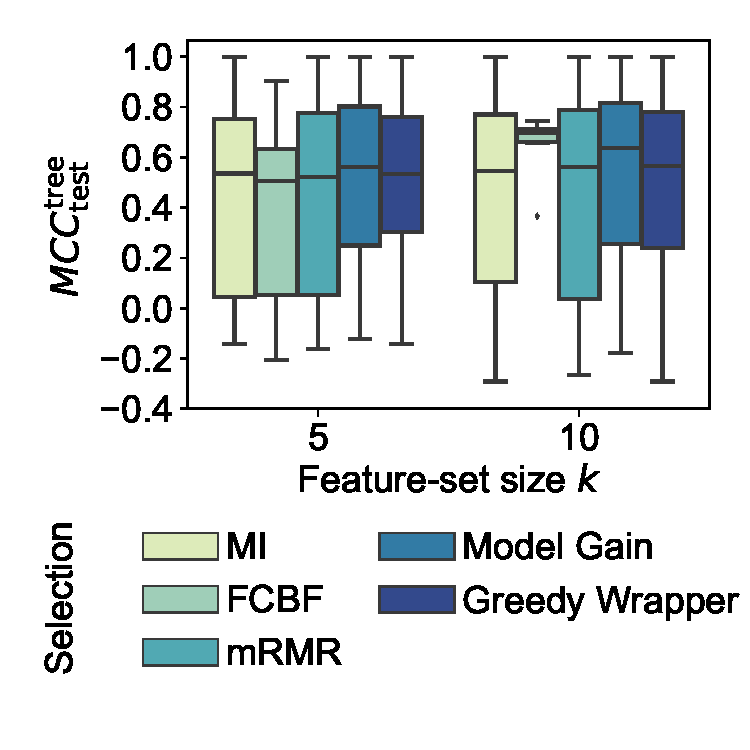
\includegraphics[width=\textwidth, trim=15 35 5 15, clip]{plots/afs-impact-fs-method-k-decision-tree-test-mcc.pdf}
		\caption{Test-set prediction performance by feature-set size~$k$.}
		\label{fig:afs:impact-fs-method-k-decision-tree-test-mcc}
	\end{subfigure}
	\hfill
	\begin{subfigure}[t]{0.48\textwidth}
		\centering
		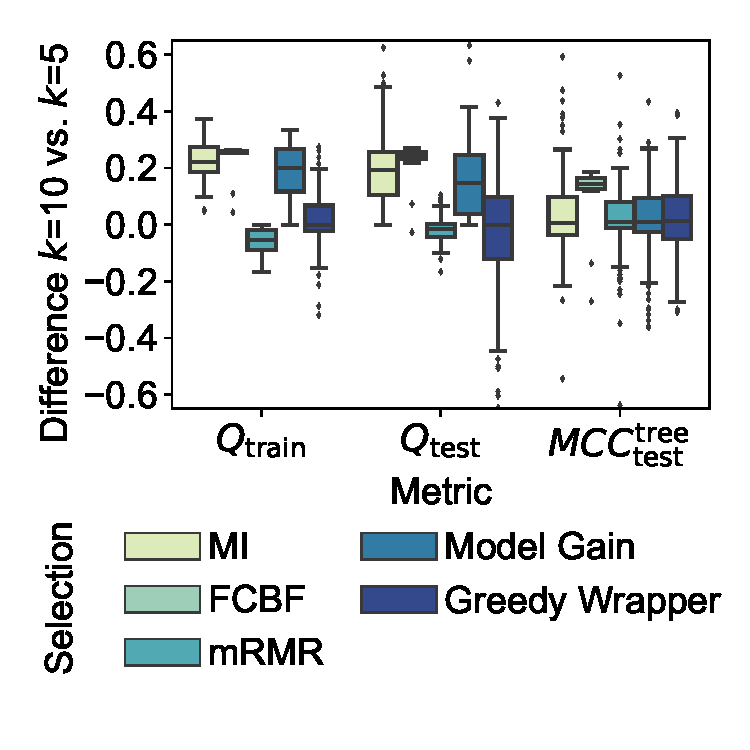
\includegraphics[width=\textwidth, trim=15 35 5 15, clip]{plots/afs-impact-fs-method-k-metric-diff.pdf}
		\caption{
			Difference in feature-set quality between $k=10$ and $k=5$ by evaluation metric.
			Y-axis is truncated to improve readability.
		}
		\label{fig:afs:impact-fs-method-k-metric-diff}
	\end{subfigure}
	\caption{
		Distribution of feature-set quality over datasets and cross-validation folds, by feature-selection method.
		Results from the original feature sets of solver-based sequential search.
	}
	\label{fig:afs:impact-fs-method-k-quality}
\end{figure}

\paragraph{Prediction performance}

The five feature-selection methods in our experiments employ different objective functions~$Q(s,X,y)$, so comparing objective values between them does not make sense.
However, we can analyze the prediction performance of the obtained feature sets.
Figure~\ref{fig:afs:impact-fs-method-k-decision-tree-test-mcc} displays the distribution of a decision tree's test-set MCC on the original feature sets, i.e., without constraints, for the feature-selection methods.
The mean test-set MCC is 0.53 for \emph{Model Gain} and \emph{Greedy Wrapper}, 0.47 for \emph{MI}, 0.46 for \emph{mRMR}, and 0.43 for \emph{FCBF}.
Thus, the analyses of alternative feature sets in Sections~\ref{sec:afs:evaluation:search-methods} and~\ref{sec:afs:evaluation:parameters} focus on \emph{Model Gain} while still discussing the remaining feature-selection methods.

The univariate, model-free method \emph{MI} keeps up surprisingly well with more sophisticated methods.
It uses the same objective function as \emph{Model Gain} but obtains its feature qualities from a bivariate dependency measure rather than a prediction model.

\emph{Greedy Wrapper} uses prediction performance to assess feature-set quality but employs a search heuristic instead of optimizing globally.
In particular, it performed 661 iterations on average to determine the original feature sets.
However, the number of possible feature sets is higher, e.g., already $\binom{15}{5} = 3003$ for the lowest-dimensional dataset in our evaluation (cf.~Table~\ref{tab:afs:datasets}) and $k=5$.
The still high prediction performance comes at the expense of high runtime (cf.~Table~\ref{tab:afs:impact-search-fs-method-optimization-time}), so we prefer \emph{Model Gain} for later evaluations.

\emph{FCBF}'s results may be taken with a grain of salt:
The original feature set in solver-based sequential search is already infeasible, i.e., no solution satisfied the constraints, in 71\% of the cases for \emph{FCBF} but never for the other feature-selection methods.
Over all solver-based search runs, even 89\% of the feature sets were infeasible for \emph{FCBF} but only 18\% for \emph{Model Gain}.
In particular, the combination of feature-correlation constraints in our formulation of \emph{FCBF} (cf.~Equation~\ref{eq:afs:fcbf}) with a cardinality constraint (cf.~Equation~\ref{eq:syn:cardinality}), i.e., enforcing a feature-set size~$k$, may make the problem infeasible, especially if~$k$ gets larger.

\paragraph{Influence of feature-set size~$k$}

One could expect larger feature sets to exhibit a higher feature-set quality than smaller ones, but the picture in our experiments is more nuanced.
In particular, quality may not increase proportionally with $k$ or may even decrease.
As Figure~\ref{fig:afs:impact-fs-method-k-metric-diff} shows for the original feature sets of solver-based sequential search, \emph{MI} and \emph{Model Gain} exhibit an increase of the training-set objective value~$Q_\text{train}$ from~$k=5$ to~$k=10$, i.e., the difference depicted in Figure~\ref{fig:afs:impact-fs-method-k-metric-diff} is positive.
As these objectives are monotonic and the feature qualities are non-negative, a decrease in the training-set objective value is impossible.
In contrast, \emph{Greedy Wrapper} with its black-box objective does not necessarily benefit from more features.
The latter insight also applies to \emph{mRMR}, which normalizes its objective with the number of selected features and penalizes feature redundancy.
For \emph{FCBF}, the fraction of feasible feature sets changes considerably from $k=5$ to $k=10$, so the overall quality between these two settings should not be compared.
As Figure~\ref{fig:afs:impact-fs-method-k-metric-diff} also displays, the benefit of larger feature sets is even less clear for prediction performance.
In particular, all feature-selection methods except \emph{FCBF} show a median difference in test-set MCC close to zero when comparing $k=5$ to $k=10$.

\subsection{Search Methods for Alternatives}
\label{sec:afs:evaluation:search-methods}

\begin{figure}[t]
	\centering
	\begin{subfigure}[t]{\textwidth}
		\centering
		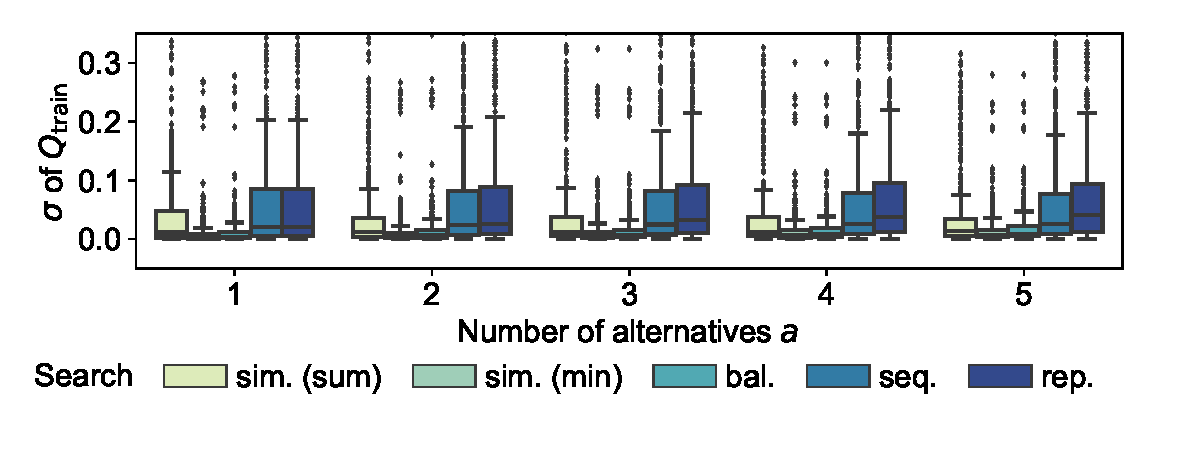
\includegraphics[width=\textwidth, trim=15 25 35 15, clip]{plots/afs-impact-search-stddev-train-objective.pdf}
		\caption{Training-set objective value.}
		\label{fig:afs:impact-search-stddev-train-objective}
	\end{subfigure}
	\\ \vspace{\baselineskip}
	\begin{subfigure}[t]{\textwidth}
		\centering
		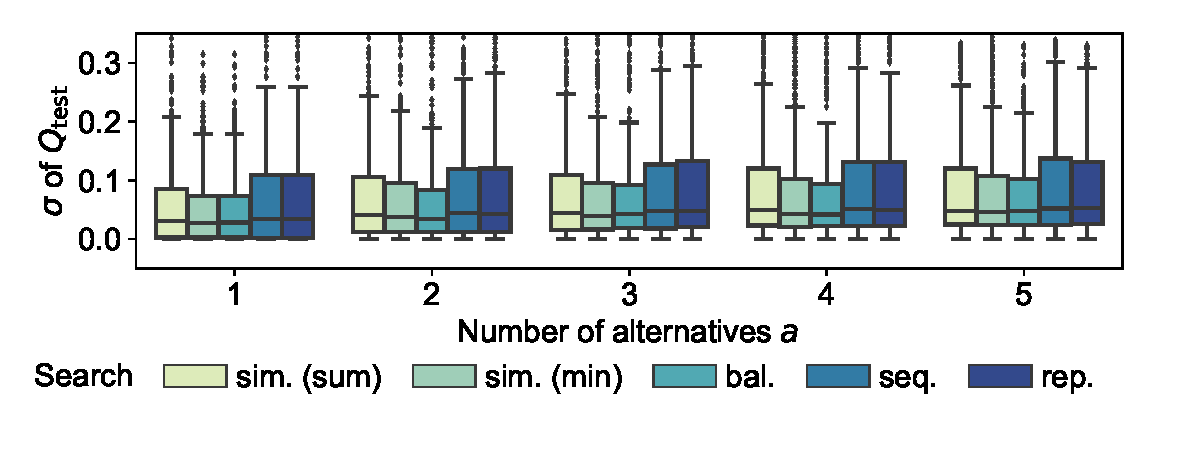
\includegraphics[width=\textwidth, trim=15 25 35 15, clip]{plots/afs-impact-search-stddev-test-objective.pdf}
		\caption{Test-set objective value.}
		\label{fig:afs:impact-search-stddev-test-objective}
	\end{subfigure}
	\\ \vspace{\baselineskip}
	\begin{subfigure}[t]{\textwidth}
		\centering
		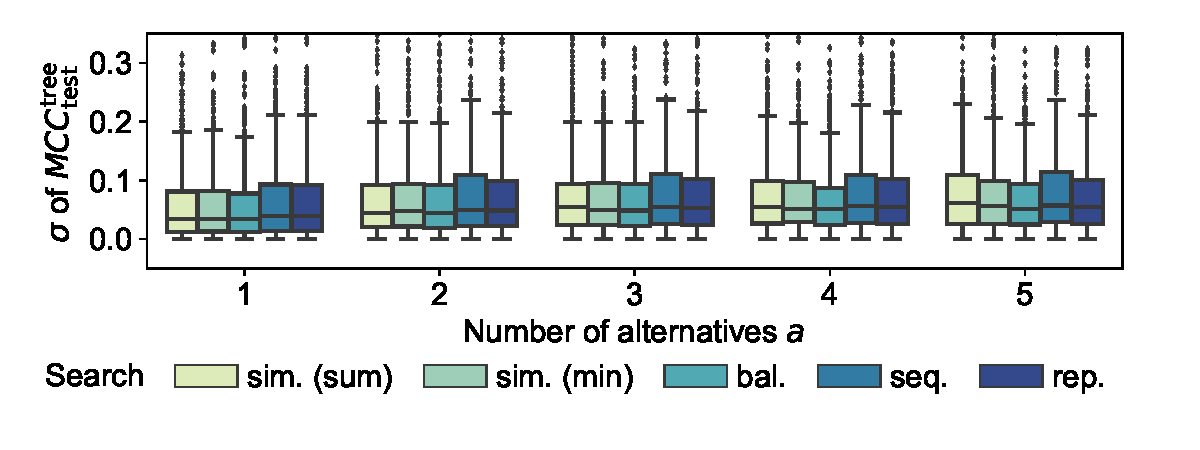
\includegraphics[width=\textwidth, trim=15 25 35 15, clip]{plots/afs-impact-search-stddev-decision-tree-test-mcc.pdf}
		\caption{Test-set prediction performance.}
		\label{fig:afs:impact-search-stddev-decision-tree-test-mcc}
	\end{subfigure}
	\caption{
		Distribution of standard deviation of feature-set quality within search runs over datasets, cross-validation-folds, and~$\tau$, by search method for alternatives and number of alternatives~$a$.
		Results with \emph{Model Gain} as the feature-selection method and $k=5$.
		Excludes search settings where at least one combination of search method and~$a$ yielded no valid solution.
		Y-axes are truncated to improve readability.
	}
	\label{fig:afs:impact-search-stddev-quality}
\end{figure}

\paragraph{Variance in feature-set quality}

As expected, the search method influences how much the training-set objective value~$Q$ varies between multiple alternatives obtained for the same experimental settings, i.e., within one search run for alternatives.
Figure~\ref{fig:afs:impact-search-stddev-train-objective} visualizes this result for \emph{Model Gain} as the feature-selection method and $k=5$.
The figure shows how the standard deviation of the training-set objective value within individual search runs for alternatives is distributed over other experimental settings, e.g., datasets and cross-validation folds.
In particular, the quality of multiple alternatives varies more if they are found by solver-based sequential search rather than solver-based simultaneous search.
For solver-based simultaneous search, min-aggregation yields considerably more homogeneous feature-set quality than sum-aggregation.
These findings apply to all white-box feature-selection methods but not \emph{Greedy Wrapper}.

The heuristic search method \emph{Greedy Balancing} yields a small variance of training-set objective value within search runs, only slightly higher than for solver-based simultaneous search with min-aggregation.
In contrast, \emph{Greedy Replacement} rather mimics solver-based sequential search, having a substantial variance of quality.
Additionally, the variance of \emph{Greedy Replacement} noticeably grows with the number of alternatives~$a$.

As Figures~\ref{fig:afs:impact-search-stddev-test-objective} and~\ref{fig:afs:impact-search-stddev-decision-tree-test-mcc} show, the variance of feature-set quality differs considerably less between the search methods on the test set, for the objective value as well as prediction performance.
This effect might result from overfitting:
Even if the training-set quality is similar, some alternatives might generalize better than others.
Thus, this variance caused by overfitting could alleviate the effect caused by the choice of search method.

\begin{figure}[t]
	\centering
	\begin{subfigure}[t]{\textwidth}
		\centering
		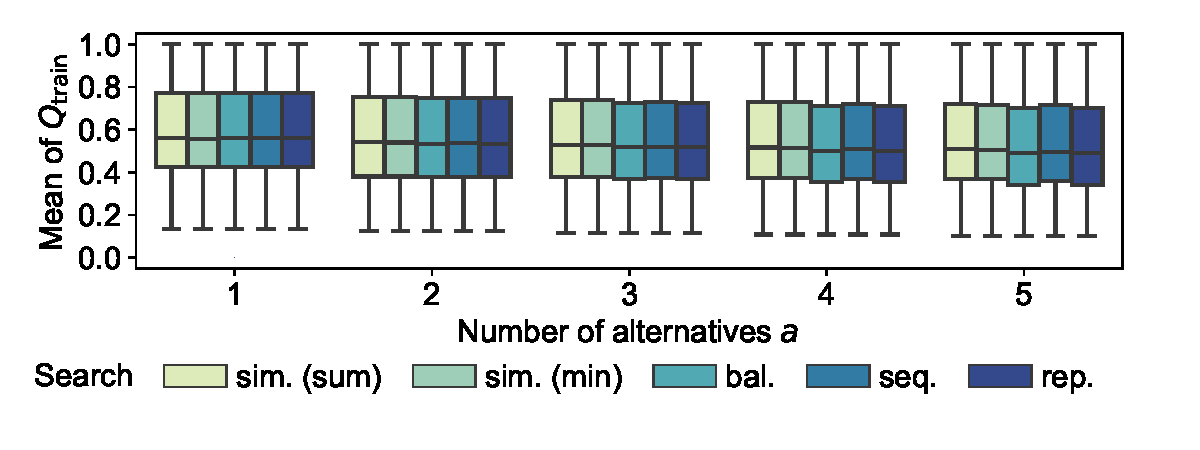
\includegraphics[width=\textwidth, trim=15 25 35 15, clip]{plots/afs-impact-search-mean-train-objective.pdf}
		\caption{Training-set objective value.}
		\label{fig:afs:impact-search-mean-train-objective}
	\end{subfigure}
	\\ \vspace{\baselineskip}
	\begin{subfigure}[t]{\textwidth}
		\centering
		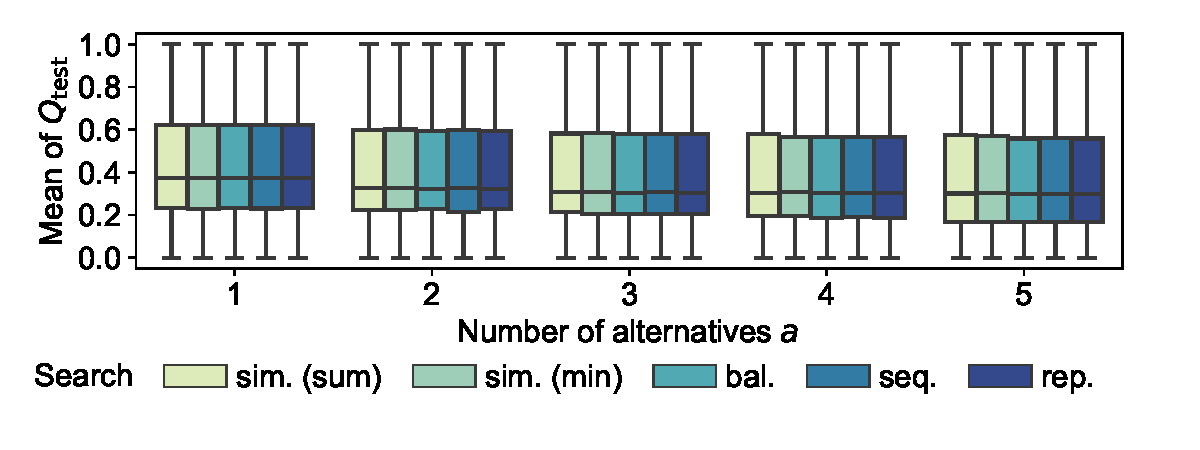
\includegraphics[width=\textwidth, trim=15 25 35 15, clip]{plots/afs-impact-search-mean-test-objective.pdf}
		\caption{Test-set objective value.}
		\label{fig:afs:impact-search-mean-test-objective}
	\end{subfigure}
	\\ \vspace{\baselineskip}
	\begin{subfigure}[t]{\textwidth}
		\centering
		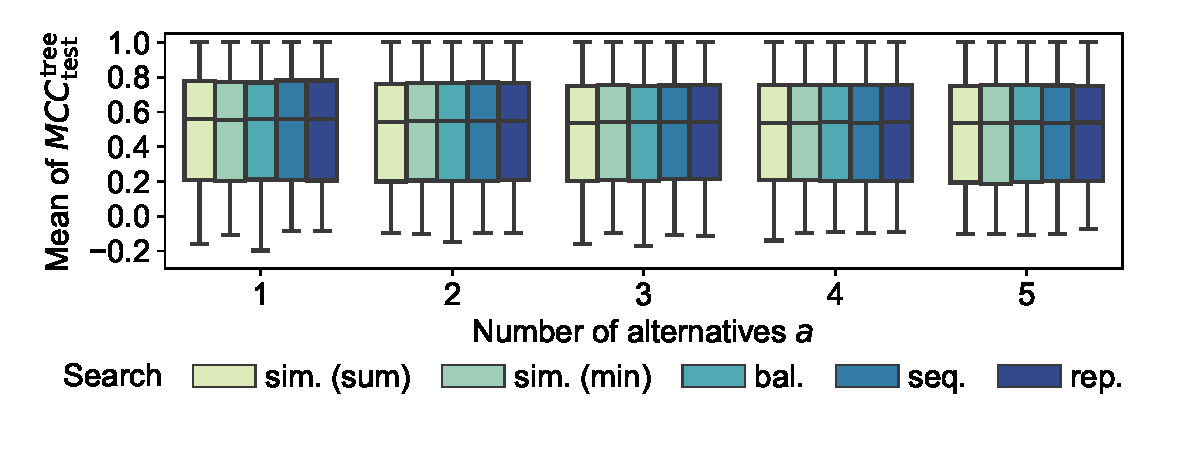
\includegraphics[width=\textwidth, trim=15 25 35 14, clip]{plots/afs-impact-search-mean-decision-tree-test-mcc.pdf}
		\caption{Test-set prediction performance.}
		\label{fig:afs:impact-search-mean-decision-tree-test-mcc}
	\end{subfigure}
	\caption{
		Distribution of mean feature-set quality within search runs over datasets, cross-validation-folds, and~$\tau$, by search method for alternatives and number of alternatives~$a$.
		Results with \emph{Model Gain} as the feature-selection method and $k=5$.
		Excludes search settings where at least one combination of search method and~$a$ yielded no valid solution.
		Y-axes are truncated to improve readability.
	}
	\label{fig:afs:impact-search-mean-quality}
\end{figure}

\paragraph{Average value of feature-set quality}

While obtaining alternatives of homogeneous quality can be one goal of simultaneous search, another selling point would be obtaining alternatives of higher average quality than sequential search.
However, this potential advantage rarely materialized in our experiments.
In particular, Figure~\ref{fig:afs:impact-search-mean-train-objective} compares the distribution of the mean training-set objective value in search runs with \emph{Model Gain} as the feature-selection method and $k=5$.
We observe that all search methods yield very similar overall distributions of average feature-set quality.
Comparing solver-based sequential and simultaneous search on each experimental setting separately and then aggregating also shows a mean quality difference close to zero.
Further, outliers can occur in both directions, i.e., either solver-based search method may yield higher quality.

The mean test-set objective value in Figure~\ref{fig:afs:impact-search-mean-test-objective} and the mean test-set prediction performance in Figure~\ref{fig:afs:impact-search-mean-decision-tree-test-mcc} also exhibit a negligible quality difference between the search methods.
Finally, the other four feature-selection methods besides \emph{Model Gain} do not show a general quality advantage of solver-based simultaneous search either.

\begin{figure}[t]
	\centering
	\begin{subfigure}[t]{0.48\textwidth}
		\centering
		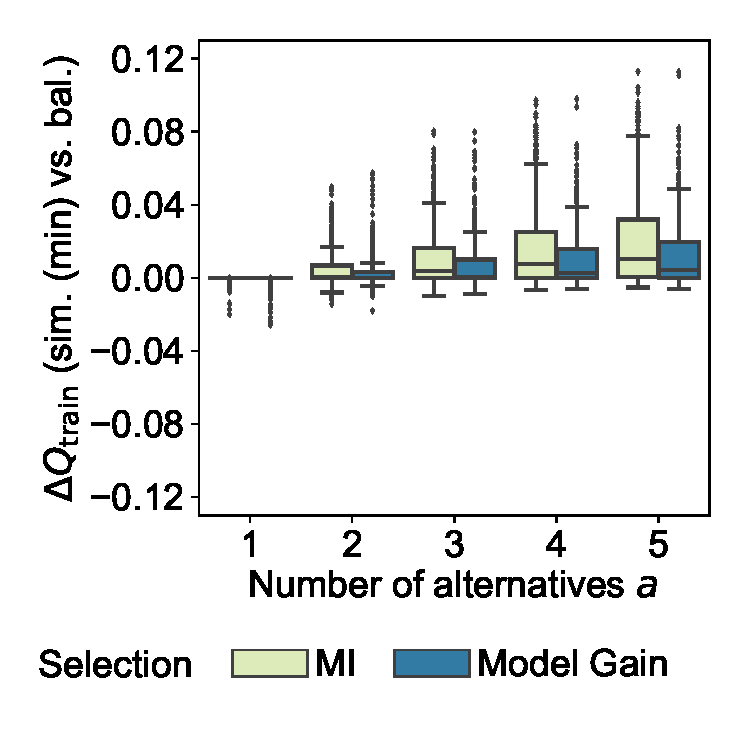
\includegraphics[width=\textwidth, trim=15 30 15 15, clip]{plots/afs-impact-search-heuristics-metric-diff-sim-num-alternatives.pdf}
		\caption{
			Difference between solver-based simultaneous (min-aggregation) search and \emph{Greedy Balancing}, by the number of alternatives~$a$.
		}
		\label{fig:afs:impact-search-heuristics-metric-diff-sim-num-alternatives}
	\end{subfigure}
	\hfill
	\begin{subfigure}[t]{0.48\textwidth}
		\centering
		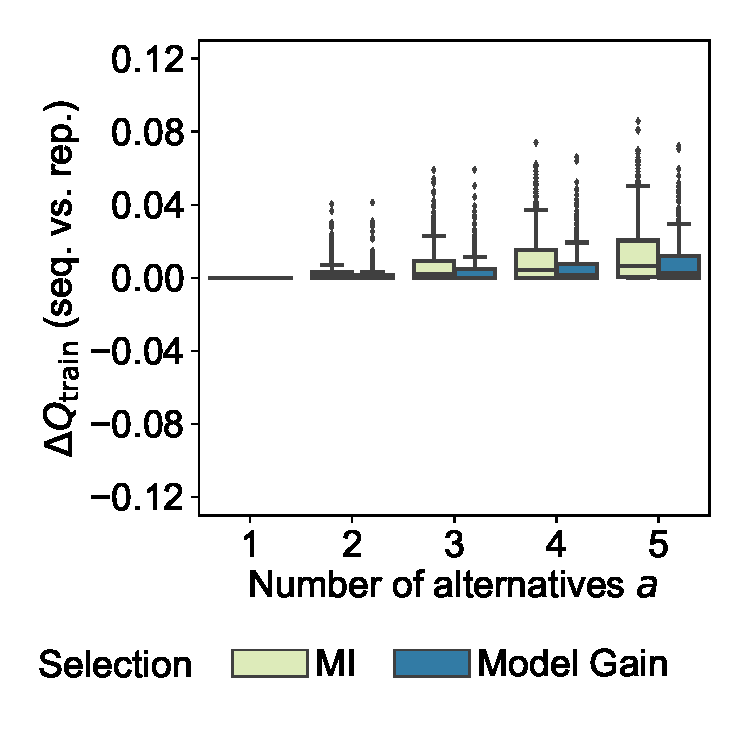
\includegraphics[width=\textwidth, trim=15 30 15 15, clip]{plots/afs-impact-search-heuristics-metric-diff-seq-num-alternatives.pdf}
		\caption{
			Difference between solver-based sequential search and \emph{Greedy Replacement}, by the number of alternatives~$a$.
		}
		\label{fig:afs:impact-search-heuristics-metric-diff-seq-num-alternatives}
	\end{subfigure}
	\\ \vspace{\baselineskip}
	\begin{subfigure}[t]{0.48\textwidth}
		\centering
		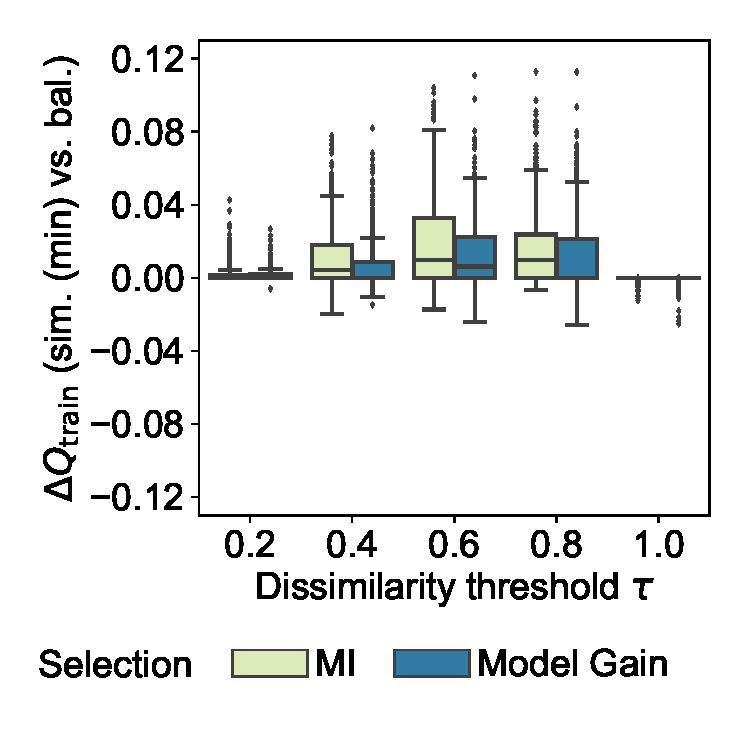
\includegraphics[width=\textwidth, trim=15 30 15 15, clip]{plots/afs-impact-search-heuristics-metric-diff-sim-tau.pdf}
		\caption{
			Difference between solver-based simultaneous (min-aggregation) search and \emph{Greedy Balancing}, by the dissimilarity threshold~$\tau$.
		}
		\label{fig:afs:impact-search-heuristics-metric-diff-sim-tau}
	\end{subfigure}
	\hfill
	\begin{subfigure}[t]{0.48\textwidth}
		\centering
		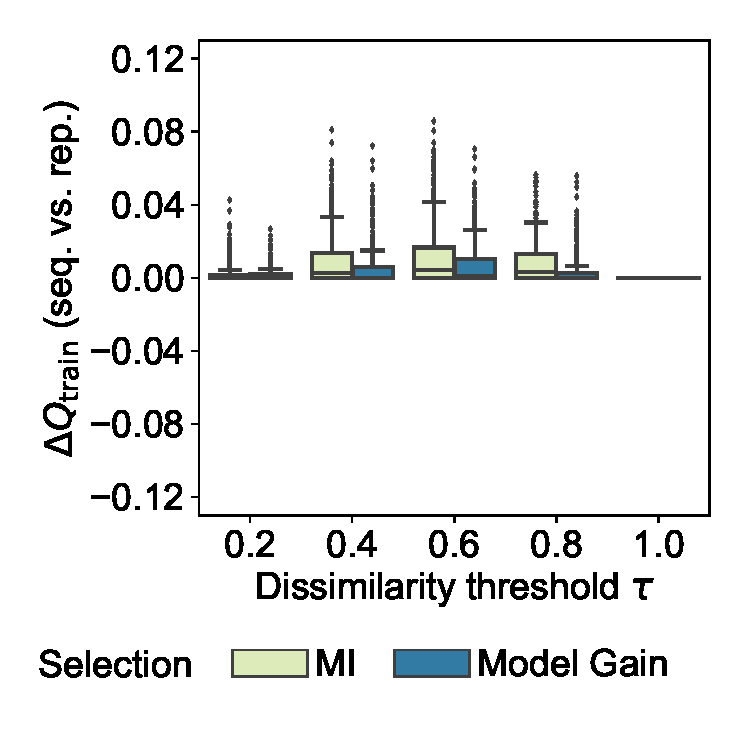
\includegraphics[width=\textwidth, trim=15 30 15 15, clip]{plots/afs-impact-search-heuristics-metric-diff-seq-tau.pdf}
		\caption{
			Difference between solver-based sequential search and \emph{Greedy Replacement}, by the dissimilarity threshold~$\tau$.
		}
		\label{fig:afs:impact-search-heuristics-metric-diff-seq-tau}
	\end{subfigure}
	\caption{
		Distribution of difference in mean training feature-set quality within a search run between solver-based and heuristic search methods over remaining experimental settings, by feature-selection method.
		Results with $k=5$.
		Excludes search settings where at least one combination of search method and~$a$ yielded no valid solution.
	}
	\label{fig:afs:impact-search-heuristics-metric-diff}
\end{figure}

\paragraph{Quality difference of heuristics}

We now look closer at the quality difference between solver-based and heuristic search.
Figure~\ref{fig:afs:impact-search-heuristics-metric-diff} compares the mean training feature-set quality within search runs for each experimental setting separately.
In particular, we compare solver-based simultaneous search with min-aggregation to \emph{Greedy Balancing} (cf.~Figures~\ref{fig:afs:impact-search-heuristics-metric-diff-sim-num-alternatives} and~\ref{fig:afs:impact-search-heuristics-metric-diff-sim-tau}) and solver-based sequential search to \emph{Greedy Replacement} (cf.~Figures~\ref{fig:afs:impact-search-heuristics-metric-diff-seq-num-alternatives} and~\ref{fig:afs:impact-search-heuristics-metric-diff-seq-tau}).
Positive values in Figure~\ref{fig:afs:impact-search-heuristics-metric-diff} express that solver-based search yields higher quality; negative values favor heuristic search.
The latter can occur if solver-based search yields suboptimal solutions due to timeouts, as we analyze later (cf.~Table~\ref{tab:afs:impact-search-fs-method-optimization-status}).

Figures~\ref{fig:afs:impact-search-heuristics-metric-diff-sim-num-alternatives} and~\ref{fig:afs:impact-search-heuristics-metric-diff-seq-num-alternatives} compare solver-based and heuristic search over the number of alternatives~$a$.
For $a=1$, solver-based and heuristic search yield the same mean training feature-set quality except when timeouts occur.
The more alternatives are desired, the more advantageous a solver-based search is quality-wise.
As in prior analyses, the picture is less clear on the test set, which shows a smaller quality difference here.
Further, the difference in mean training feature-set quality between \emph{Greedy Balancing} and solver-based simultaneous search (cf.~Figure~\ref{fig:afs:impact-search-heuristics-metric-diff-sim-num-alternatives}) grows faster with~$a$ than between \emph{Greedy Replacement} and solver-based sequential search (cf.~Figure~\ref{fig:afs:impact-search-heuristics-metric-diff-seq-num-alternatives}).
As an explanation, consider that optimal simultaneous search may generally develop a quality advantage over optimal sequential search for more alternatives.
\emph{Greedy Balancing} selects the same features as \emph{Greedy Replacement}, i.e., a sequential search heuristic, and only distributes them differently into feature sets, yielding the same mean feature-set quality.

Figures~\ref{fig:afs:impact-search-heuristics-metric-diff-sim-tau} and~\ref{fig:afs:impact-search-heuristics-metric-diff-seq-tau} compare solver-based and heuristic search over the dissimilarity threshold~$\tau$.
Unlike for~$a$, the difference in mean training feature-set quality between solver-based and heuristic search does not increase over the whole range of~$\tau$ but shows an increase followed by a decrease.
In particular, $\tau=1$ allows the two heuristic search methods to reach the same mean training feature-set quality as the solver-based methods.
This observation corresponds to our theoretical result that optimizing the summed quality of alternatives with~$\tau=1$ admits polynomial-time algorithms (cf.~Proposition~\ref{prop:afs:complexity-partitioning-sum}).

\begin{table}[t]
	\centering
	\caption{
		Frequency of optimization statuses (cf.~Section~\ref{sec:afs:experimental-design:evaluation}) over datasets, cross-validation folds, $a$, and $\tau$, by feature-selection method and search method for alternatives.
		Results with $k=5$, $a \in \{1,2,3,4,5\}$, and excluding \emph{Greedy Wrapper}, which does not use the solver for optimizing.
		Each row adds up to 100\%.
	}
	\begin{tabular}{llrrrr}
		\toprule
		\multirow{2}{*}{Feature selection} & \multirow{2}{*}{Search} & \multicolumn{4}{c}{Optimization status} \\
		\cmidrule(lr){3-6}
		& & Infeasible & Not solved & Feasible & Optimal \\
		\midrule
		FCBF & seq. & 74.51\% & 0.00\% & 0.00\% & 25.49\% \\
		FCBF & sim. (min) & 73.07\% & 0.00\% & 1.60\% & 25.33\% \\
		FCBF & sim. (sum) & 73.07\% & 0.00\% & 2.19\% & 24.75\% \\
		MI & bal. & 0.00\% & 9.20\% & 90.80\% & 0.00\% \\
		MI & rep. & 0.00\% & 9.20\% & 90.80\% & 0.00\% \\
		MI & seq. & 4.93\% & 0.00\% & 0.00\% & 95.07\% \\
		MI & sim. (min) & 4.67\% & 0.00\% & 9.33\% & 86.00\% \\
		MI & sim. (sum) & 4.67\% & 0.00\% & 3.04\% & 92.29\% \\
		Model Gain & bal. & 0.00\% & 9.20\% & 90.80\% & 0.00\% \\
		Model Gain & rep. & 0.00\% & 9.20\% & 90.80\% & 0.00\% \\
		Model Gain & seq. & 4.93\% & 0.00\% & 0.00\% & 95.07\% \\
		Model Gain & sim. (min) & 4.67\% & 0.00\% & 5.28\% & 90.05\% \\
		Model Gain & sim. (sum) & 4.67\% & 0.00\% & 1.87\% & 93.47\% \\
		mRMR & seq. & 4.88\% & 0.00\% & 9.55\% & 85.57\% \\
		mRMR & sim. (min) & 4.67\% & 0.00\% & 48.64\% & 46.69\% \\
		mRMR & sim. (sum) & 4.67\% & 0.00\% & 67.04\% & 28.29\% \\
		\bottomrule
	\end{tabular}
	\label{tab:afs:impact-search-fs-method-optimization-status}
\end{table}

\begin{table}[t]
	\centering
	\caption{
		Frequency of optimization statuses (cf.~Section~\ref{sec:afs:experimental-design:evaluation}) over datasets, cross-validation folds, feature-selection methods, and~$\tau$, by number of alternatives~$a$.
		Results from solver-based simultaneous search with sum-aggregation, $k=5$, and excluding \emph{Greedy Wrapper}.
		Each row adds up to 100\%.
	}
	\begin{tabular}{rrrr}
		\toprule
		\multirow{2}{*}{$a$} & \multicolumn{3}{c}{Optimization status} \\
		\cmidrule(lr){2-4}
		& Infeasible & Feasible & Optimal \\
		\midrule
		1 & 16.10\% & 7.60\% & 76.30\% \\
		2 & 17.50\% & 13.27\% & 69.23\% \\
		3 & 20.00\% & 20.20\% & 59.80\% \\
		4 & 27.00\% & 21.43\% & 51.57\% \\
		5 & 28.23\% & 30.17\% & 41.60\% \\
		\bottomrule
	\end{tabular}
	\label{tab:afs:impact-num-alternatives-optimization-status}
\end{table}

\paragraph{Optimization status}

Suboptimal search results are one reason why solver-based simultaneous search fails to consistently beat solver-based sequential search quality-wise.
For \emph{Greedy Wrapper}, the search is heuristic per se and does not cover the entire search space.
For all feature-selection methods, the solver can time out.
Table~\ref{tab:afs:impact-search-fs-method-optimization-status} shows that solver-based simultaneous search has a higher likelihood of timeouts than solver-based sequential search, likely due to the larger size of the optimization problem (cf.~Table~\ref{tab:afs:seq-sim-comparison}).
In particular, for up to five alternatives and $k=5$, all solver-based sequential searches for \emph{FCBF}, \emph{MI}, and \emph{Model Gain} finished within the timeout, i.e., yielded the optimal feature set or ascertained infeasibility, while \emph{mRMR} had about 10\% timeouts.
In contrast, for solver-based simultaneous search with sum-aggregation, all feature-selection methods experience timeouts:
1--3\% of the searches for \emph{FCBF}, \emph{MI}, and \emph{Model Gain}, and 67\% of the searches for \emph{mRMR} found a feasible solution but could not prove optimality.
Such timeout-affected simultaneous solutions can be worse than optimal sequential solutions.

\emph{mRMR} is especially prone to suboptimal solutions, likely because it has a more complex objective (cf.~Equation~\ref{eq:afs:mrmr-linear}) than~\emph{MI} and \emph{Model Gain}.
\emph{FCBF} often results in infeasible optimization problems since its constraints, which prevent the selection of redundant features (cf.~Equation~\ref{eq:afs:fcbf}), might prevent finding any valid feature set of size~$k$.
Min-aggregation instead of sum-aggregation in solver-based simultaneous search exhibits more timeouts for \emph{MI} and \emph{Model Gain} but less for \emph{FCBF} and \emph{mRMR}.
Still, solver-based sequential search incurs fewer timeouts for all of these four feature-selection methods.

Also, note that the fraction of timeouts in solver-based simultaneous search strongly depends on the number of alternatives~$a$, as Table~\ref{tab:afs:impact-num-alternatives-optimization-status} displays:
For $k=5$ and sum-aggregation, roughly 8\% of the white-box searches timed out for~$a=1$, but 20\% for~$a=3$ and 30\% for~$a=5$.
While we grant solver-based simultaneous searches proportionally more time for multiple alternatives (cf.~Section~\ref{sec:afs:experimental-design:approaches:alternatives}), the observed increase in timeouts suggests that runtime increases super-proportionally with~$a$, as we analyze later.

For the heuristic search methods, Table~\ref{tab:afs:impact-search-fs-method-optimization-status} shows that \emph{Greedy Replacement} more often did not find a valid alternative (9.20\%) than solver-based sequential search (4.93\%).
A similar phenomenon occurred for \emph{Greedy Balancing} (9.20\%) compared to solver-based simultaneous search (4.67\%).
Such a result can be expected since both heuristic search methods stop early as soon as each feature is part of at least one alternative.

\begin{table}[t]
	\centering
	\caption{
		Mean optimization time over datasets, cross-validation folds, $a$, and $\tau$, by feature-selection method and search method for alternatives.
		Results with $k=5$ and $a \in \{1,2,3,4,5\}$.
	}
	\begin{tabular}{lrrrrr}
		\toprule
		\multirow{2}{*}{Feature selection} & \multicolumn{5}{c}{Optimization time} \\
		\cmidrule(lr){2-6}
		& Bal. & Rep. & Seq. & Sim. (min) & Sim. (sum) \\
		\midrule
		FCBF & --- & --- & 0.22~s & 11.41~s & 12.62~s \\
		Greedy Wrapper & --- & --- & 52.62~s & 68.39~s & 70.36~s \\
		MI & 0.00~s & 0.00~s & 0.03~s & 47.39~s & 24.56~s \\
		Model Gain & 0.00~s & 0.00~s & 0.03~s & 30.38~s & 19.08~s \\
		mRMR & --- & --- & 33.59~s & 156.00~s & 189.25~s \\
		\bottomrule
	\end{tabular}
	\label{tab:afs:impact-search-fs-method-optimization-time}
\end{table}

\begin{table}[t]
	\centering
	\caption{
		Mean optimization time over datasets, cross-validation folds, and $\tau$, by number of alternatives and feature-selection method.
		Results from solver-based simultaneous search with sum-aggregation and $k=5$.
	}
	\begin{tabular}{lrrrrr}
		\toprule
		\multirow{2}{*}{$a$} & \multicolumn{5}{c}{Optimization time} \\
		\cmidrule(lr){2-6}
		& FCBF & Greedy Wrapper & MI & Model Gain & mRMR \\
		\midrule
		1 & 0.45~s & 28.44~s & 0.03~s & 0.02~s & 44.68~s \\
		2 & 0.86~s & 41.76~s & 0.09~s & 0.08~s & 117.62~s \\
		3 & 2.97~s & 62.70~s & 0.30~s & 0.27~s & 208.14~s \\
		4 & 13.32~s & 96.65~s & 3.68~s & 3.47~s & 258.19~s \\
		5 & 45.52~s & 122.26~s & 118.72~s & 91.58~s & 317.63~s \\
		\bottomrule
	\end{tabular}
	\label{tab:afs:impact-num-alternatives-fs-method-optimization-time}
\end{table}

\paragraph{Optimization time}

As Table~\ref{tab:afs:impact-search-fs-method-optimization-time} shows, solver-based sequential search is faster on average than solver-based simultaneous search for all five feature-selection methods.
In particular, the difference is up to three orders of magnitude for the four white-box feature-selection methods.
Further, \emph{FCBF}, \emph{MI}, and \emph{Model Gain} experience a dramatic increase in optimization time with the number of alternatives~$a$ in solver-based simultaneous search, as Table~\ref{tab:afs:impact-num-alternatives-fs-method-optimization-time} displays.
In contrast, the runtime increase is considerably less for solver-based sequential search, which shows an approximately linear trend with the number of alternatives.

Table~\ref{tab:afs:impact-search-fs-method-optimization-time} also shows that the optimization time of the heuristic search methods for \emph{MI} and \emph{Model Gain} is negligible.
In particular, \emph{Greedy Replacement} and \emph{Greedy Balancing} never took longer than 1~ms per search run for alternatives.
These results highlight the runtime advantage of the heuristics, particularly of \emph{Greedy Balancing} for simultaneous search.

An interesting question for practitioners is how the runtime relates to~$n$, the number of features in the dataset.
One could expect a positive correlation since the problem instance increases with~$n$.
Roughly speaking, this trend appears in our experimental data indeed.
However, the observed trend is rather noisy, particularly for solver-based simultaneous search, and some higher-dimensional datasets even show lower average runtimes than lower-dimensional ones.
This result indicates that other factors than~$n$ influence runtime as well, e.g., other experimental settings or the solver's internal search heuristics.

Based on all results described in this section, we focus on solver-based sequential search in the next section.
In particular, it was significantly faster than solver-based simultaneous search while yielding similar feature-set quality.

\subsection{User Parameters \texorpdfstring{$a$ And $\tau$}{}}
\label{sec:afs:evaluation:parameters}

\begin{figure}[p]
	\centering
	\begin{subfigure}[t]{0.48\textwidth}
		\centering
		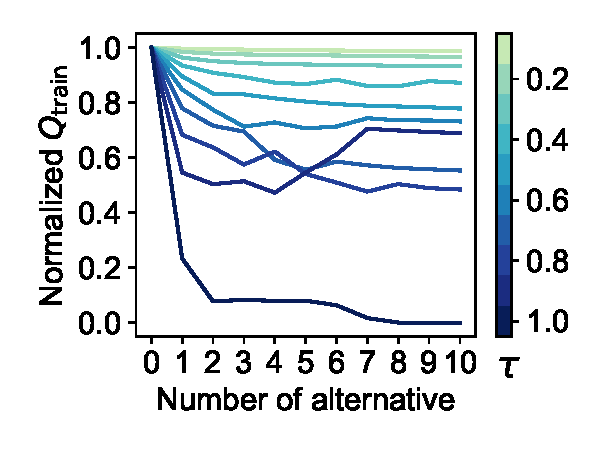
\includegraphics[width=\textwidth, trim=15 17 10 15, clip]{plots/afs-impact-num-alternatives-tau-train-objective-max.pdf}
		\caption{
			Training-set objective value.
			Infeasible feature sets excluded.
		}
		\label{fig:afs:impact-num-alternatives-tau-train-objective-max}
	\end{subfigure}
	\hfill
	\begin{subfigure}[t]{0.48\textwidth}
		\centering
		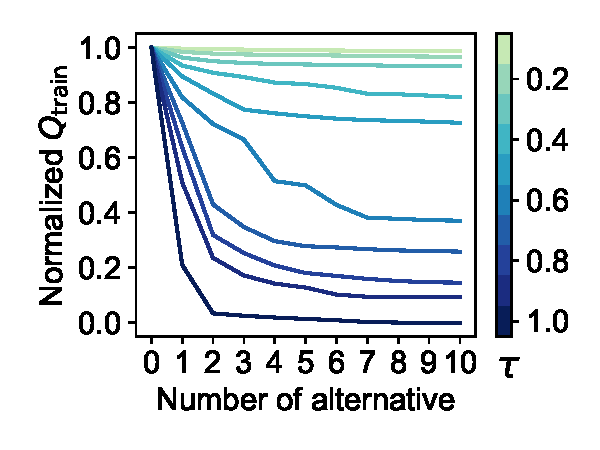
\includegraphics[width=\textwidth, trim=15 17 10 15, clip]{plots/afs-impact-num-alternatives-tau-train-objective-max-fillna.pdf}
		\caption{
			Training-set objective value.
			Infeasible feature sets assigned a quality of~0.
		}
		\label{fig:afs:impact-num-alternatives-tau-train-objective-max-fillna}
	\end{subfigure}
	\\ \vspace{\baselineskip}
	\begin{subfigure}[t]{0.48\textwidth}
		\centering
		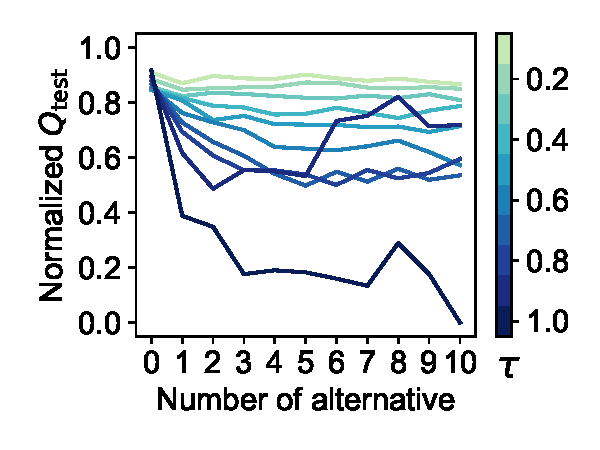
\includegraphics[width=\textwidth, trim=15 17 10 15, clip]{plots/afs-impact-num-alternatives-tau-test-objective-max.pdf}
		\caption{
			Test-set objective value.
			Infeasible feature sets excluded.
		}
		\label{fig:afs:impact-num-alternatives-tau-test-objective-max}
	\end{subfigure}
	\hfill
	\begin{subfigure}[t]{0.48\textwidth}
		\centering
		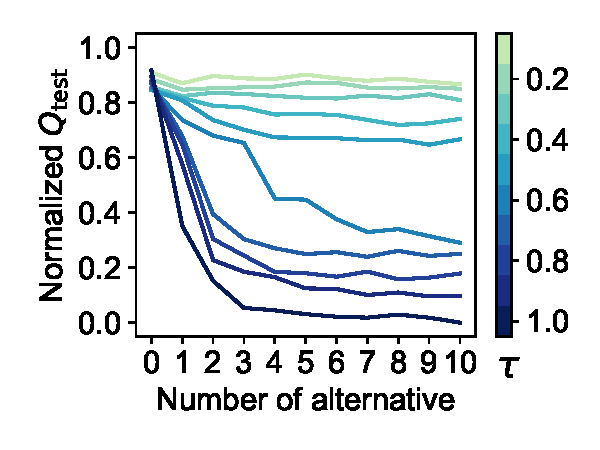
\includegraphics[width=\textwidth, trim=15 17 10 15, clip]{plots/afs-impact-num-alternatives-tau-test-objective-max-fillna.pdf}
		\caption{
			Test-set objective value.
			Infeasible feature sets assigned a quality of~0.
		}
		\label{fig:afs:impact-num-alternatives-tau-test-objective-max-fillna}
	\end{subfigure}
	\\ \vspace{\baselineskip}
	\begin{subfigure}[t]{0.48\textwidth}
		\centering
		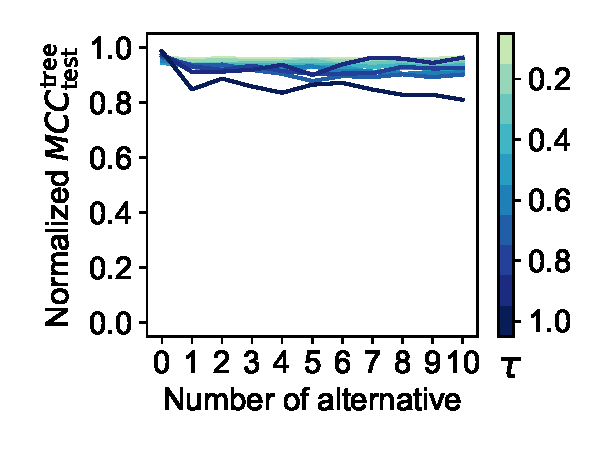
\includegraphics[width=\textwidth, trim=15 17 10 15, clip]{plots/afs-impact-num-alternatives-tau-decision-tree-test-mcc-max.pdf}
		\caption{
			Test-set prediction performance.
			Infeasible feature sets excluded.
		}
		\label{fig:afs:impact-num-alternatives-tau-decision-tree-test-mcc-max}
	\end{subfigure}
	\hfill
	\begin{subfigure}[t]{0.48\textwidth}
		\centering
		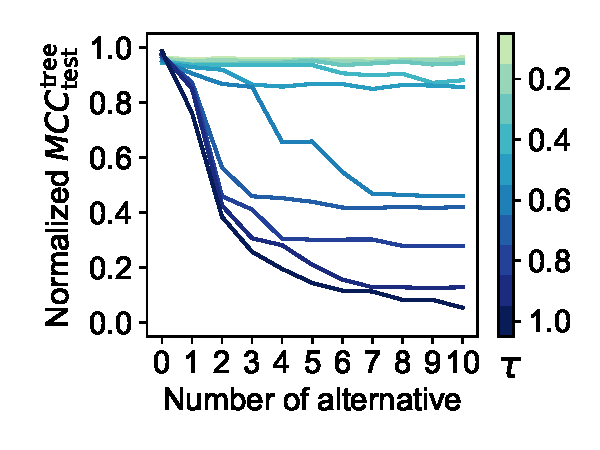
\includegraphics[width=\textwidth, trim=15 17 10 15, clip]{plots/afs-impact-num-alternatives-tau-decision-tree-test-mcc-max-fillna.pdf}
		\caption{
			Test-set prediction performance.
			Infeasible feature sets assigned a quality of~0.
		}
		\label{fig:afs:impact-num-alternatives-tau-decision-tree-test-mcc-max-fillna}
	\end{subfigure}
	\caption{
		Mean feature-set quality over datasets and cross-validation folds, max-normalized per search run for alternatives, by the number of alternative and dissimilarity threshold~$\tau$.
		Results from solver-based sequential search with \emph{Model Gain} as the feature-selection method and $k=10$.
	}
	\label{fig:afs:impact-num-alternatives-tau-quality}
\end{figure}

\paragraph{Feature-set quality}

Higher values of the two user parameters introduce more (for~$a$) or stronger (for~$\tau$) constraints into the optimization problem of alternative feature selection.
Thus, one would expect a corresponding decrease in feature-set quality.
Figure~\ref{fig:afs:impact-num-alternatives-tau-quality} illustrates this trend for \emph{Model Gain} as the feature-selection method and $k=10$.
Since the maximum feature-set quality varies among datasets, we max-normalize quality in this figure.
In particular, we set the highest feature-set quality in each search run for alternatives to~1 and scale the other feature-set qualities accordingly.
For prediction performance in terms of MCC, we shift its range from~$[-1,1]$ to~$[0,1]$ before normalization.

Figure~\ref{fig:afs:impact-num-alternatives-tau-quality} shows that multiple alternatives may have a similar quality.
Further, the training-set objective value (cf.~Figure~\ref{fig:afs:impact-num-alternatives-tau-train-objective-max}) decreases most from the original feature set, i.e., the zeroth alternative, to the first alternative, but less beyond.
Also, the decrease strongly depends on the dissimilarity threshold~$\tau$.
For a low dissimilarity threshold like $\tau=0.1$, the training-set objective value barely drops over the number of alternatives.
Additionally, note that Figure~\ref{fig:afs:impact-num-alternatives-tau-quality} averages the normalized feature-set quality over multiple datasets.
In our experiments, datasets with more features tend to experience a smaller decrease in quality over~$a$ and~$\tau$.
As higher-dimensional datasets offer more options for alternatives, this observation makes sense.
However, this effect is not guaranteed since datasets with many features could also contain many useless features instead of interesting alternatives.

The overall decrease in quality is slightly less pronounced for the test-set objective value (Figure~\ref{fig:afs:impact-num-alternatives-tau-test-objective-max}) than on the training set (Figure~\ref{fig:afs:impact-num-alternatives-tau-train-objective-max}) since overfitting might occur.
In particular, the original feature set can even have lower test-set quality than the subsequent alternatives.
The trend becomes even less clear for prediction performance, which varies little over~$a$ and~$\tau$ in our experiments (cf.~Figure~\ref{fig:afs:impact-num-alternatives-tau-decision-tree-test-mcc-max}).
In general, the optimization objective~$Q$ may only partially indicate actual prediction performance since the former may use a simplified feature-set quality criterion.
Indeed, the correlation between optimization objective~$Q$ and prediction MCC is only weak to moderate in our experiments.

\begin{figure}[t]
	\centering
	\begin{subfigure}[t]{0.48\textwidth}
		\centering
		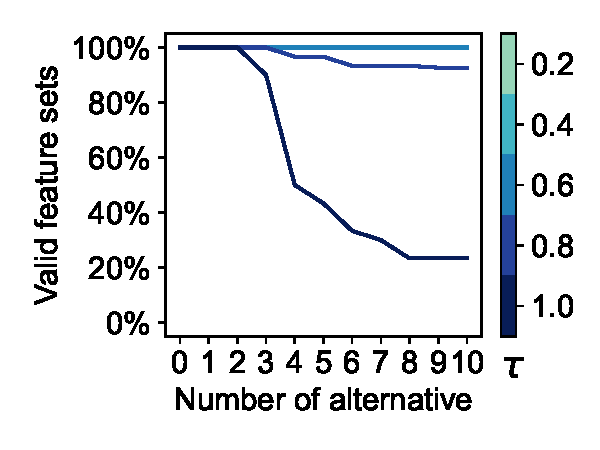
\includegraphics[width=\textwidth, trim=15 15 10 15, clip]{plots/afs-impact-num-alternatives-tau-optimization-status-k-5.pdf}
		\caption{Feature-set size~$k=5$.}
		\label{fig:afs:impact-num-alternatives-tau-optimization-status-k-5}
	\end{subfigure}
	\hfill
	\begin{subfigure}[t]{0.48\textwidth}
		\centering
		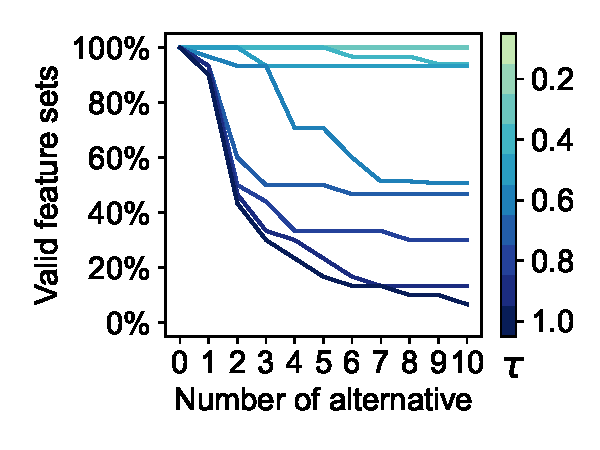
\includegraphics[width=\textwidth, trim=15 15 10 15, clip]{plots/afs-impact-num-alternatives-tau-optimization-status-k-10.pdf}
		\caption{Feature-set size~$k=10$.}
		\label{fig:afs:impact-num-alternatives-tau-optimization-status-k-10}
	\end{subfigure}
	\caption{
		Frequency of optimization runs yielding a valid feature set over datasets and cross-validation folds, by the number of alternative and dissimilarity threshold~$\tau$.
		Results from solver-based sequential search with \emph{Model Gain} as the feature-selection method.
	}
	\label{fig:afs:impact-num-alternatives-tau-optimization-status}
\end{figure}

\paragraph{Optimization status}

The previous observations refer to the quality of the found feature sets.
However, the more alternatives one desires and the more they should differ, the likelier an infeasible optimization problem is.
Figure~\ref{fig:afs:impact-num-alternatives-tau-optimization-status} visualizes the fraction of valid feature sets over the number of alternatives and dissimilarity threshold~$\tau$, showing the expected trend.
Additionally, Figures~\ref{fig:afs:impact-num-alternatives-tau-train-objective-max-fillna},~\ref{fig:afs:impact-num-alternatives-tau-test-objective-max-fillna}, and~\ref{fig:afs:impact-num-alternatives-tau-decision-tree-test-mcc-max-fillna} display the same data as Figures~\ref{fig:afs:impact-num-alternatives-tau-train-objective-max},~\ref{fig:afs:impact-num-alternatives-tau-test-objective-max}, and~\ref{fig:afs:impact-num-alternatives-tau-decision-tree-test-mcc-max} but with the quality of infeasible feature sets set to zero instead of excluding these feature sets from evaluation.
Consequently, the decrease in feature-set quality over~$a$ and~$\tau$ is noticeably stronger.
In contrast, if only considering valid feature sets, the mean quality in our experiments can increase over the number of alternatives, e.g., as visible in Figures~\ref{fig:afs:impact-num-alternatives-tau-train-objective-max} and~\ref{fig:afs:impact-num-alternatives-tau-test-objective-max} for $\tau=0.9$.
This counterintuitive phenomenon can occur because some datasets run out of valid feature sets sooner than others, so the average quality may be determined for different sets of datasets at each number of alternatives.

\begin{figure}[t]
	\centering
	\begin{subfigure}[t]{0.48\textwidth}
		\centering
		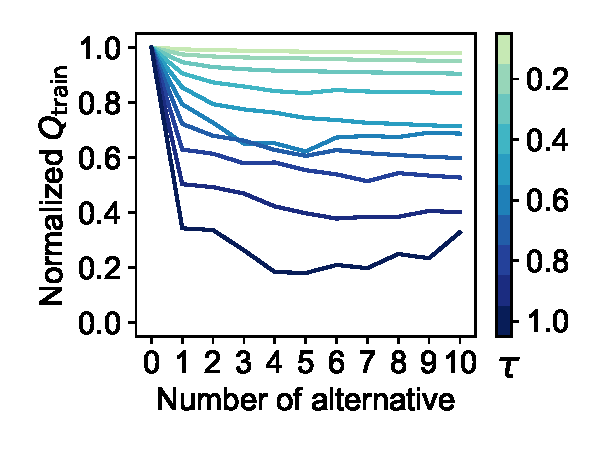
\includegraphics[width=\textwidth, trim=15 17 10 15, clip]{plots/afs-impact-num-alternatives-tau-train-objective-max-mi.pdf}
		\caption{
			\emph{MI} as the feature-selection method.
		}
		\label{fig:afs:impact-num-alternatives-tau-train-objective-max-mi}
	\end{subfigure}
	\hfill
	\begin{subfigure}[t]{0.48\textwidth}
		\centering
		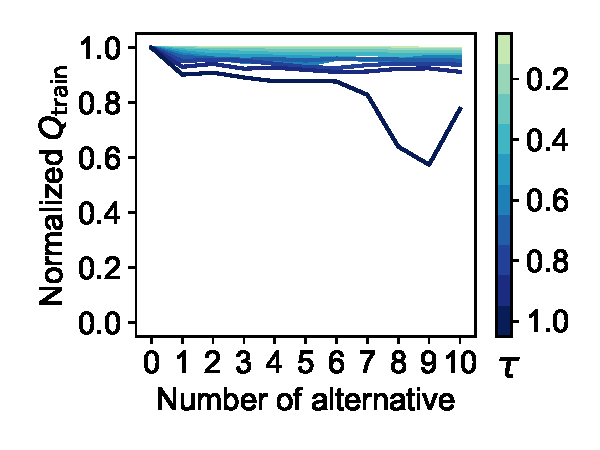
\includegraphics[width=\textwidth, trim=15 17 10 15, clip]{plots/afs-impact-num-alternatives-tau-train-objective-max-mrmr.pdf}
		\caption{
			\emph{mRMR} as the feature-selection method.
		}
		\label{fig:afs:impact-num-alternatives-tau-train-objective-max-mrmr}
	\end{subfigure}
	\\ \vspace{\baselineskip}
	\begin{subfigure}[t]{0.48\textwidth}
		\centering
		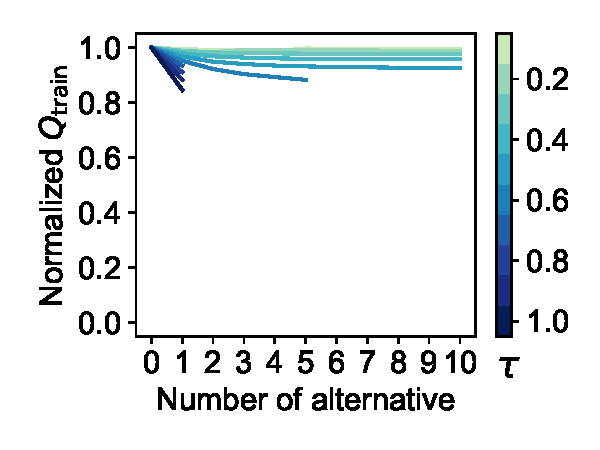
\includegraphics[width=\textwidth, trim=15 17 10 15, clip]{plots/afs-impact-num-alternatives-tau-train-objective-max-fcbf.pdf}
		\caption{
			\emph{FCBF} as the feature-selection method.
		}
		\label{fig:afs:impact-num-alternatives-tau-train-objective-max-fcbf}
	\end{subfigure}
	\hfill
	\begin{subfigure}[t]{0.48\textwidth}
		\centering
		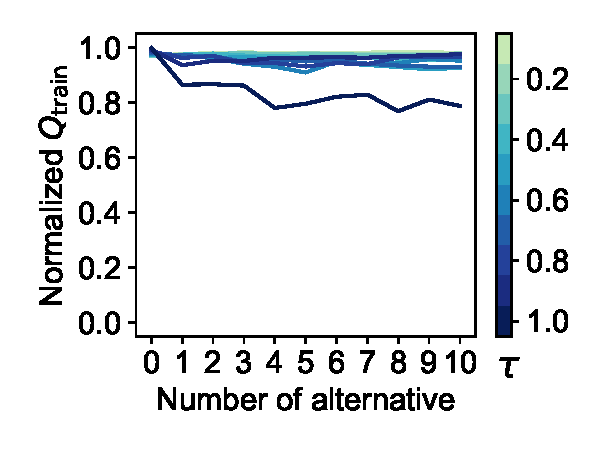
\includegraphics[width=\textwidth, trim=15 17 10 15, clip]{plots/afs-impact-num-alternatives-tau-train-objective-max-greedy-wrapper.pdf}
		\caption{
			\emph{Greedy Wrapper} as the feature-selection method.
		}
		\label{fig:afs:impact-num-alternatives-tau-train-objective-max-greedy-wrapper}
	\end{subfigure}
	\caption{
		Mean training-set objective value over datasets and cross-validation folds, max-normalized per search run for alternatives, by the number of alternative and dissimilarity threshold~$\tau$.
		Results from solver-based sequential search with $k=10$.
		Infeasible feature sets excluded.
	}
	\label{fig:afs:impact-num-alternatives-tau-train-objective-fs-method}
\end{figure}

\paragraph{Influence of feature-selection method}

While we discussed \emph{Model Gain} before, the decrease in objective value over~$a$ and~$\tau$ occurs to different extents for the other feature-selection methods in our experiments, as Figure~\ref{fig:afs:impact-num-alternatives-tau-train-objective-fs-method} displays.
In this figure, we shifted the objectives of \emph{Greedy Wrapper} and \emph{mRMR} to~$[0, 1]$ before max-normalization since their original range is~$[-1,1]$.
\emph{MI} (cf.~Figure~\ref{fig:afs:impact-num-alternatives-tau-train-objective-max-mi}) shows a similar behavior as \emph{Model Gain} (cf.~Figure~\ref{fig:afs:impact-num-alternatives-tau-train-objective-max}), which may result from both feature-selection methods using the same objective function, though with different feature qualities.
In contrast, \emph{mRMR} (cf.~Figure~\ref{fig:afs:impact-num-alternatives-tau-train-objective-max-mrmr}) exhibits a considerably smaller effect of increasing~$\tau$.
For \emph{FCBF} (cf.~Figure~\ref{fig:afs:impact-num-alternatives-tau-train-objective-max-fcbf}), the additional constraints on feature-feature correlation (cf.~Equation~\ref{eq:afs:fcbf}) cause many infeasible results (cf.~Table~\ref{tab:afs:impact-search-fs-method-optimization-status}), so we cannot determine the average feature-set quality for some combinations of~$a$ and~$\tau$.
For \emph{Greedy Wrapper} (cf.~Figure~\ref{fig:afs:impact-num-alternatives-tau-train-objective-max-greedy-wrapper}), $a$ and~$\tau$ barely make any difference, which may be explained by the heuristic, inexact search procedure.

\subsection{Summary}
\label{sec:afs:evaluation:summary}

\paragraph{Feature-selection methods (cf.~Section~\ref{sec:afs:evaluation:feature-selection})}

Among the feature-selection methods, \emph{Model Gain} yielded the best average prediction performance.
The simple univariate \emph{MI} also turned out competitive, while \emph{Greedy Wrapper} and \emph{mRMR} required high optimization times, and our constraint-based version of \emph{FCBF} yielded many infeasible solutions.
Selecting $k=10$ instead of $k=5$ features had only a small impact on prediction performance, so users may stick to smaller feature-set sizes if such a setting benefits interpretability.

\paragraph{Search methods for alternatives (cf.~Section~\ref{sec:afs:evaluation:search-methods})}

Solver-based simultaneous search, particularly with min-aggregation, considerably reduced the variance of the training-set objective value over alternatives compared to solver-based sequential search, as we desired.
However, results were less clear on the test set and when using prediction performance to measure feature-set quality.
Further, the average quality of alternatives was similar to solver-based sequential search.
In addition, the latter was considerably faster and led to fewer solver timeouts, particularly when increasing the number of alternatives.
Also, sequential search allows users to stop searching after each alternative.

The heuristic search methods \emph{Greedy Replacement} and \emph{Greedy Balancing} for univariate feature qualities achieved a good feature-set quality relative to solver-based search, particularly for a low number of alternatives and on the test set.
For a high number of alternatives, the training feature-set quality may differ more and the heuristics may stop early despite the existence of further alternatives.
As a positive point, both the heuristics' runtime was negligible.
Also, \emph{Greedy Balancing} achieved a low variance of training-set objective value between alternatives, similar to solver-based simultaneous search with min-aggregation.

\paragraph{User parameters $a$ and $\tau$ (cf.~Section~\ref{sec:afs:evaluation:parameters})}

Feature-set quality tended to decrease with a higher number of alternatives~$a$ and dissimilarity threshold~$\tau$, so these parameters give users control over alternatives.
The decrease was highest from the original feature set to the first alternative but smaller beyond, resulting in multiple alternatives of similar quality.
Also, the decrease was more prominent on the training set than on the test set.
Further, the strength of this decrease depended on the feature-selection method;
\emph{MI} and \emph{Model Gain} showed the largest effect.
Independent from the feature-selection method, the frequency of infeasible solutions increased with~$a$ and~$\tau$ due to stronger constraints.

\chapter{Discovering Sparse and Alternative Subgroup Descriptions}
\label{sec:csd}

\section{Overview}
\label{sec:csd:overview}

\paragraph{Scope}

In this chapter, we move to the field of subgroup discovery (cf.~Definition~\ref{def:csd:subgroup-discovery}).
Building on our work regarding constrained feature selection (cf.~Chapter~\ref{sec:syn}), we investigate constraints on features in subgroup descriptions:
We limit the number of selected features and search for alternative solutions, adapting the approach from Chapter~\ref{sec:afs}.
Both these constraint types make subgroup discovery more user-centric.

\paragraph{Contributions}

Our contribution in this chapter is fivefold:

(1) We formalize subgroup discovery as a Satisfiability Modulo Theories (SMT) optimization problem.
This novel white-box formulation admits a solver-based search for subgroups and allows integrating constraints in a declarative manner.

(2) We formalize two constraint types for this optimization problem: feature-cardinality constraints and alternative subgroup descriptions.
\emph{Feature-cardinality constraints} limit the number of selected features, i.e., features used in subgroup descriptions.
Thus, the subgroup descriptions become \emph{sparse}, which increases their interpretability at the potential expense of subgroup quality.
\emph{Alternative subgroup descriptions} should use different features than a given subgroup description but cover a similar set of data objects.
We allow users to control alternatives with two parameters, i.e., the number of alternatives and a dissimilarity threshold.
We integrate both constraint types into our white-box problem formulation.

(3) We describe how to integrate these two constraint types into three existing heuristic search methods and two novel baselines for subgroup discovery.
The latter are faster and simpler than the former, so they may serve as additional reference points for future experimental studies on subgroup discovery.

(4) We analyze the time complexity of the subgroup-discovery problem with each of these two constraint types and prove several $\mathcal{NP}$-completeness results.

(5) We conduct comprehensive experiments with 27 binary-classification datasets from the Penn Machine Learning Benchmarks (PMLB)~\cite{olson2017pmlb, romano2021pmlb}.
We compare solver-based and heuristic subgroup-discovery methods in different experimental scenarios:
without constraints, with a feature-cardinality constraint, and for searching alternative subgroup descriptions.
In particular, we evaluate the runtime of subgroup discovery and the quality of the discovered subgroups.
We also analyze how the subgroup quality in solver-based search depends on the timeout of the solver.
Section~\ref{sec:csd:evaluation:summary} summarizes key results.

\paragraph{Materials}

We publish all our code and experimental data online (cf.~Section~\ref{sec:introduction:materials}).

\paragraph{Prior works}

The content of this chapter bases on the following prior work:
%
\begin{itemize}
	\item \fullcite{bach2024using}
\end{itemize}

\paragraph{Chapter outline}

The remainder of this chapter is structured as follows:
Section~\ref{sec:csd:baselines} introduces two baselines for subgroup discovery.
Section~\ref{sec:csd:approach} describes and analyzes constrained subgroup discovery.
Section~\ref{sec:csd:experimental-design} outlines our experimental design.
Section~\ref{sec:csd:evaluation} presents the corresponding experimental results.

\section{Baselines}
\label{sec:csd:baselines}

In this section, we propose and analyze two baselines for subgroup discovery, \emph{MORS} (cf.~Section~\ref{sec:csd:baselines:mors}) and \emph{Random Search} (cf.~Section~\ref{sec:csd:baselines:random-search}).
They are conceptually simpler than existing heuristic search methods (cf.~Section~\ref{sec:fundamentals:subgroup-discovery:methods}) and serve as further reference points in our experiments.
While they technically also are heuristics, we use the term \emph{baselines} to refer to these two methods specifically.

\begin{algorithm}[t]
	\DontPrintSemicolon
	\KwIn{Dataset~$X \in \mathbb{R}^{m \times n}$, \newline
		Prediction target~$y \in \{0, 1\}^m$
	}
	\KwOut{Subgroup bounds~$\mathit{lb}, \mathit{ub} \in \{\mathbb{R} \cup \{-\infty, +\infty\}\}^n$}
	\BlankLine
	\For{$j \leftarrow 1$ \KwTo $n$}{
		$\mathit{lb}_j \leftarrow \min\limits_{\substack{i \in \{1, \dots, m\} \\ y_i = 1}} X_{ij}$\; \label{al:csd:mors:line:bounds-start}
		$\mathit{ub}_j \leftarrow \max\limits_{\substack{i \in \{1, \dots, m\} \\ y_i = 1}} X_{ij}$\; \label{al:csd:mors:line:bounds-end}
		\lIf{$\mathit{lb}_j = \min_{i \in \{1, \dots, m\}} X_{ij}$}{$\mathit{lb}_j \leftarrow -\infty$} \label{al:csd:mors:line:bounds-infty-start}
		\lIf{$\mathit{ub}_j = \max_{i \in \{1, \dots, m\}} X_{ij}$}{$\mathit{ub}_j \leftarrow + \infty$} \label{al:csd:mors:line:bounds-infty-end}
	}
	\For{$j \notin \text{get\_permissible\_feature\_idxs(\dots)}$}{ \label{al:csd:mors:line:reset-start} \label{al:csd:mors:line:permissible-features}
		$(\mathit{lb}_j,~ \mathit{ub}_j) \leftarrow (-\infty, +\infty)$\; \label{al:csd:mors:line:reset-end}
	}
	\Return{$\mathit{lb}, \mathit{ub}$}
	\caption{\emph{MORS} for subgroup discovery.}
	\label{al:csd:mors}
\end{algorithm}

\subsection{MORS}
\label{sec:csd:baselines:mors}

This baseline builds on the following definition:
%
\begin{definition}[Minimal Optimal-Recall Subgroup (MORS)]
	Given a dataset $X \in \mathbb{R}^{m \times n}$ with prediction target~$y \in \{0, 1\}^m$,
	the \emph{Minimal Optimal-Recall Subgroup (MORS)} is the subgroup (cf.~Definition~\ref{def:csd:subgroup}) whose lower and upper bounds of each feature correspond to the minimum and maximum value of that feature over all positive data objects (i.e., with $y_i = 1$) from the dataset~$X$.
	\label{def:csd:mors}
\end{definition}
%
The definition ensures that all positive data objects are contained in the subgroup.
Thus, the evaluation metric \emph{recall}, i.e., the fraction of positive data objects becoming subgroup members, reaches its \emph{optimal} value of~1.
At the same time, raising the lower bounds or lowering the upper bounds would exclude positive data objects from the subgroup.
In this sense, the set of subgroup members is \emph{minimal}.
The corresponding subgroup description is unique and solves the following variant of the subgroup-discovery problem:
%
\begin{definition}[Minimal-optimal-recall-subgroup discovery]
	Given a dataset $X \in \mathbb{R}^{m \times n}$ with prediction target~$y \in \{0, 1\}^m$,
	\emph{minimal-optimal-recall-subgroup discovery} is the problem of finding a subgroup (cf.~Definition~\ref{def:csd:subgroup}) that contains as few negative data objects (i.e., with $y_i = 0$) as possible but all positive data objects (i.e., with $y_i = 1$) from the dataset~$X$.
	\label{def:csd:minimal-optimal-recall-subgroup-discovery}
\end{definition}
%
I.e., the problem minimizes the number of false positives subject to producing no false negatives.
Equivalently, it maximizes the number of true negatives, i.e., negative data objects excluded from the subgroup, subject to producing no false negatives.

Algorithm~\ref{al:csd:mors} outlines the procedure to determine the \emph{MORS} bounds.
Slightly deviating from Definition~\ref{def:csd:mors}, but consistent to~Algorithm~\ref{al:csd:prim}, \emph{MORS} replaces all non-excluding bounds with infinity (Lines~\ref{al:csd:mors:line:bounds-infty-start}--\ref{al:csd:mors:line:bounds-infty-end}).
Further, if only certain features are permissible to be bounded, as we discuss later, we reset the bounds of the remaining features (Lines~\ref{al:csd:mors:line:reset-start}--\ref{al:csd:mors:line:reset-end}).

Since \emph{MORS} only needs to iterate over all data objects and features once to determine the minima and maxima, the time complexity of this algorithm is~$O(m \cdot n)$.
This places minimal-optimal-recall-subgroup discovery in the complexity class~$\mathcal{P}$:
%
\begin{proposition}[Complexity of minimal-optimal-recall-subgroup discovery]
	The problem of minimal-optimal-recall-subgroup discovery (cf.~Definition~\ref{def:csd:minimal-optimal-recall-subgroup-discovery}) can be solved in~$O(m \cdot n)$.
	\label{prop:csd:complexity-unconstrained-minimal-optimal-recall-subgroup-discovery}
\end{proposition}

Interestingly, a kind of inverted problem definition, the \textsc{Maximum Box} problem, is $\mathcal{NP}$-hard~\cite{eckstein2002maximum}.
The latter problem maximizes the number of true positives, i.e., positive data objects in the subgroup, subject to no false positives, i.e., optimal precision.

For complexity proofs later in this dissertation, we define another variant of the subgroup-discovery problem based on another particular type of subgroups~\cite{meeng2014rocsearch}:
%
\begin{definition}[Perfect subgroup]
	Given a dataset~$X \in \mathbb{R}^{m \times n}$ with prediction target~$y \in \{0, 1\}^m$,
	a \emph{perfect subgroup} is a subgroup (cf.~Definition~\ref{def:csd:subgroup}) that contains all positive data objects (i.e., with $y_i = 1$) but no negative data objects (i.e., with $y_i = 0$) from the dataset~$X$.
	\label{def:csd:perfect-subgroup}
\end{definition}
%
Perfect subgroups reach the theoretical maximum WRAcc (cf.~Equation~\ref{eq:csd:wracc-max}) but do not exist in all datasets.
Next, we define a corresponding search problem:
%
\begin{definition}[Perfect-subgroup discovery]
	Given a dataset~$X \in \mathbb{R}^{m \times n}$ with prediction target~$y \in \{0, 1\}^m$,
	\emph{perfect-subgroup discovery} is the problem of finding a perfect subgroup (cf.~Definition~\ref{def:csd:perfect-subgroup}) if it exists or determining that it does not exist.
	\label{def:csd:perfect-subgroup-discovery}
\end{definition}
%
Since \emph{MORS} helps solving this problem in~$O(m \cdot n)$, we obtain the following result:
%
\begin{proposition}[Complexity of perfect-subgroup discovery]
	The problem of perfect-subgroup discovery (cf.~Definition~\ref{def:csd:perfect-subgroup-discovery}) can be solved in~$O(m \cdot n)$.
	\label{prop:csd:complexity-unconstrained-perfect-subgroup}
\end{proposition}
%
In particular, after \emph{MORS} (cf.~Algorithm~\ref{al:csd:mors}) has found a subgroup, one only needs to check whether it contains any negative data objects.
If it does not, it is perfect, otherwise no perfect subgroup exists.
In particular, the \emph{MORS} bounds cannot be tightened to exclude negative data objects without also excluding positives, thereby violating perfection.

\begin{algorithm}[t]
	\DontPrintSemicolon
	\KwIn{Dataset~$X \in \mathbb{R}^{m \times n}$, \newline
		Prediction target~$y \in \{0, 1\}^m$, \newline
		Subgroup-quality function~$Q(\mathit{lb}, \mathit{ub}, X, y)$, \newline
		Number of iterations~$\mathit{n\_iters} \in \mathbb{N}$
	}
	\KwOut{Subgroup bounds~$\mathit{lb}, \mathit{ub} \in \{\mathbb{R} \cup \{-\infty, +\infty\}\}^n$}
	\BlankLine
	$Q^{\text{opt}} \leftarrow - \infty$\;
	\For{$\mathit{iters} \leftarrow 1$ \KwTo $\mathit{n\_iters}$}{
		\For{$j \leftarrow 1$ \KwTo $n$}{ \label{al:csd:random-search:line:sampling-start}
			$(\mathit{lb}_j,~ \mathit{ub}_j) \leftarrow (-\infty, +\infty)$\;
		}
		\For{$j \in$ get\_permissible\_feature\_idxs(\dots)}{ \label{al:csd:random-search:line:permissible-features}
			$(\mathit{lb}_j,~\mathit{ub}_j) \leftarrow$ sample\_uniformly(unique($X_{\cdot j}$)) \label{al:csd:random-search:line:sampling-end}
		}
		\If{$Q(\mathit{lb}, \mathit{ub}, X, y) > Q^{\text{opt}}$}{ \label{al:csd:random-search:line:optimum-update-start}
			$Q^{\text{opt}} \leftarrow Q(\mathit{lb}, \mathit{ub}, X, y)$\;
			$(\mathit{lb}^{\text{opt}},~ \mathit{ub}^{\text{opt}}) \leftarrow (\mathit{lb},~ \mathit{ub})$\; \label{al:csd:random-search:line:optimum-update-end}
		}
	}
	\For{$j \leftarrow 1$ \KwTo $n$}{ \label{al:csd:random-search:line:bounds-infty-start}
		\lIf{$\mathit{lb}_j^{\text{opt}} = \min_{i \in \{1, \dots, m\}} X_{ij}$}{$\mathit{lb}_j^{\text{opt}} \leftarrow -\infty$} 
		\lIf{$\mathit{ub}_j^{\text{opt}} = \max_{i \in \{1, \dots, m\}} X_{ij}$}{$\mathit{ub}_j^{\text{opt}} \leftarrow +\infty$} \label{al:csd:random-search:line:bounds-infty-end}
	}
	\Return{$\mathit{lb}^{\text{opt}},~ \mathit{ub}^{\text{opt}}$}
	\caption{\emph{Random Search} for subgroup discovery.}
	\label{al:csd:random-search}
\end{algorithm}

\subsection{Random Search}
\label{sec:csd:baselines:random-search}

Algorithm~\ref{al:csd:random-search} outlines a randomized search procedure that constitutes our second baseline.
\emph{Random Search} repeatedly generates and evaluates subgroups for a user-defined number of iterations~$\mathit{n\_iters} \in \mathbb{N}$.
Each generation step samples a lower bound and an upper bound uniformly random from the unique values for each permissible feature, leaving the remaining features unrestricted (Lines~\ref{al:csd:random-search:line:sampling-start}--\ref{al:csd:random-search:line:sampling-end}).
The algorithm tracks the best generated subgroup so far over the iterations (Lines~\ref{al:csd:random-search:line:optimum-update-start}--\ref{al:csd:random-search:line:optimum-update-end}) and finally returns it.
As for Algorithm~\ref{al:csd:prim}, \emph{Random Search} replaces all non-excluding bounds with infinity (Lines~\ref{al:csd:random-search:line:bounds-infty-start}--\ref{al:csd:random-search:line:bounds-infty-end}).

\section{Constrained Subgroup Discovery}
\label{sec:csd:approach}

In this section, we discuss subgroup discovery with constraints.
First, we frame subgroup discovery as an SMT optimization problem (cf.~Section~\ref{sec:csd:approach:smt}).
Second, we formalize and analyze feature-cardinality constraints (cf.~Section~\ref{sec:csd:approach:cardinality}).
Third, we formalize and analyze alternative subgroup descriptions (cf.~Section~\ref{sec:csd:approach:alternatives}).

\subsection{SMT Encoding of Subgroup Discovery}
\label{sec:csd:approach:smt}

To find optimal subgroups exactly, one can encode subgroup discovery as a white-box optimization problem and employ a solver.
As for constrained feature selection, this approach allows directly integrating and combining a variety of constraint types in a declarative manner.
Similar to Section~\ref{sec:syn:approach}, we propose an SMT encoding with linear real arithmetic (LRA)~\cite{barrett2018satisfiability}.
This formulation is straightforward given the problem definition (cf.~Definition~\ref{def:csd:subgroup-discovery}).
Appendix~\ref{sec:appendix:csd:milp-encoding} describes an encoding as a mixed integer linear program (MILP), which performed worse in preliminary experiments.
Beyond the scope of this dissertation, \cite{bach2024using}~outlines a \textsc{MaxSAT} encoding and how to handle categorical features.

The optimization problem consists of an objective function and constraints.

\paragraph{Objective function}

We use WRAcc as the objective, which should be maximized.
In the formula for WRAcc (cf.~Equation~\ref{eq:csd:wracc}), $m$ and $m^+$ are constants, while $m_b$ and $m_b^+$ depend on the decision variables.
The previously provided formula contains $m_b$ in the numerator and denominator, but one can reformulate it by multiplying its two factors:
%
\begin{equation}
	\text{WRAcc} = \frac{m_b^+}{m} - \frac{m_b \cdot m^+}{m^2} = \frac{m_b^+ \cdot m - m_b \cdot m^+}{m^2}
	\label{eq:csd:smt-wracc}
\end{equation}
%
In this new expression, the denominators and the factor~$m^+$ in the numerator are constant.
Thus, the whole expression is linear in~$m_b^+$ and~$m_b$.
We define these two quantities as linear expressions from binary decision variables~$b \in \{0, 1\}^m$ that denote subgroup membership.
I.e., $b_i$~expresses whether the $i$-th data object is in the subgroup.
%
\begin{equation}
	\begin{aligned}
		m_b &:= \sum_{i=1}^{m} b_i \\
		m_b^+ &:= \sum_{\substack{i \in \{1, \dots, m\} \\ y_i = 1 }} b_i \\
	\end{aligned}
	\label{eq:csd:smt-constraint-m-as-sum}
\end{equation}
%
Since the values of the target variable~$y$ are fixed, the expression for~$m_b^+$ only sums over the positive data objects.
Further, one may define $m_b^+$ and~$m_b$ as separate integer variables or directly insert their expressions into Equation~\ref{eq:csd:smt-wracc}.
We chose the latter in our implementation and therefore wrote `$:=$' in Equation~\ref{eq:csd:smt-constraint-m-as-sum} instead of using a propositional operator like `$\leftrightarrow$'.
Finally, the formula for nWRAcc (cf.~Equation~\ref{eq:csd:wracc-normalized}) is linear as well, having the same enumerator as Equation~\ref{eq:csd:smt-wracc} and a different constant in the denominator.

\paragraph{Constraints}

The subgroup membership~$b_i$ of a data object depends on the bounds of the subgroup (cf.~Definition~\ref{def:csd:subgroup}).
Thus, we define real-valued decision variables $\mathit{lb}, \mathit{ub} \in \{\mathbb{R} \cup \{-\infty, +\infty\}\}^n$ for the latter.
In particular, each feature has a lower bound and an upper bound.
The upper bounds naturally need to be at least as high as the lower bounds:
%
\begin{equation}
	\forall j \in \{1, \dots, n\}:~ \mathit{lb}_j\leq \mathit{ub}_j
	\label{eq:csd:smt-constraint-bounds-monotonic}
\end{equation}
%
A data object is a member of the subgroup if all its feature values are within the bounds:
%
\begin{equation}
	\forall i \in \{1, \dots, m\}:~ b_i\leftrightarrow \bigwedge_{j \in \{1, \dots, n\}} \left( \left( X_{ij} \geq \mathit{lb}_j \right) \land \left( X_{ij} \leq \mathit{ub}_j \right) \right)
	\label{eq:csd:smt-constraint-subgroup-membership}
\end{equation}
%
Instead of defining separate decision variables~$b_i$ and binding them to the bounds with an equivalence constraint, one could also insert the corresponding Boolean expression into the right-hand-side of Equation~\ref{eq:csd:smt-constraint-m-as-sum} directly.
In particular, $\mathit{lb}_j$ and $\mathit{ub}_j$ are the only decision variables strictly necessary for the optimization problem.
However, some constraint types on subgroups may use~$b_i$ as well, so it is helpful to have it defined explicitly.

\paragraph{Complete optimization problem}

Combining all prior definitions of decision variables, constraints, and the objective, we obtain the following SMT optimization problem:

\begin{equation}
	\begin{aligned}
		\max &\quad & Q_{\text{WRAcc}} &= \frac{m_b^+}{m} - \frac{m_b \cdot m^+}{m^2} \\
		\text{s.t.:} &\quad & m_b &:= \sum_{i=1}^{m} b_i \\
		&\quad & m_b^+ &:= \sum_{\substack{i \in \{1, \dots, m\} \\ y_i = 1 }} b_i \\
		&\quad \forall i \in \{1, \dots, m\} & b_i &\leftrightarrow \bigwedge_{j \in \{1, \dots, n\}} \left( \left( X_{ij} \geq \mathit{lb}_j \right) \land \left( X_{ij} \leq \mathit{ub}_j \right) \right) \\
		&\quad \forall j \in \{1, \dots, n\} & \mathit{lb}_j &\leq \mathit{ub}_j \\
		&\quad & b &\in \{0, 1\}^m \\
		&\quad & \mathit{lb}, \mathit{ub} &\in \{\mathbb{R} \cup \{-\infty, +\infty\}\}^n
	\end{aligned}
	\label{eq:csd:smt-problem-unconstrained-complete}
\end{equation}

We refer to this optimization problem as \emph{unconstrained subgroup discovery} in the following since it only contains constraints to define subgroup discovery per se but not the additional constraints on feature sets that we will impose later.

\paragraph{Post-processing}

In our implementation, we add a small post-processing step.
In particular, we do not use the solver-determined values of the variables $\mathit{lb}_j$ and $\mathit{ub}_j$ but the minimum and maximum feature values of all data objects in the subgroup (i.e., with $b_i=1$).
Thus, we ensure that the bounds correspond to actual feature values, consistent with the bounds returned by heuristic search methods and baselines.
Further, this choice avoids potential numerical issues caused by extracting floating-point values from the solver.
If the subgroup does not contain any data objects, we use invalid bounds (i.e., $\mathit{ub}_j = -\infty < \infty = \mathit{lb}_j$) to ensure that the subgroup remains empty even for arbitrary new data objects.

\subsection{Feature-Cardinality Constraints}
\label{sec:csd:approach:cardinality}

In this section, we discuss feature-cardinality constraints for subgroup discovery.
First, we motivate and formalize them (cf.~Section~\ref{sec:csd:approach:cardinality:concept}).
Next, we describe how to integrate them into our SMT encoding of subgroup discovery (cf.~Section~\ref{sec:csd:approach:cardinality:smt}), heuristic search methods (cf.~Section~\ref{sec:csd:approach:cardinality:heuristics}), and baselines (cf.~Section~\ref{sec:csd:approach:cardinality:baselines}).
Finally, we analyze the time complexity of subgroup discovery with this constraint type (cf.~Section~\ref{sec:csd:approach:cardinality:complexity}).

\subsubsection{Concept}
\label{sec:csd:approach:cardinality:concept}

Feature-cardinality constraints limit the number of features used in the subgroup description, rendering the latter less complex and easier to interpret~\cite{meeng2021real}.
To formalize this constraint type, we define feature selection in subgroup discovery as follows:
%
\begin{definition}[Feature selection in subgroups]
	Given a dataset~$X \in \mathbb{R}^{m \times n}$ and a subgroup (cf.~Definition~\ref{def:csd:subgroup}) with bounds~$\mathit{lb}, \mathit{ub} \in \{\mathbb{R} \cup \{-\infty, +\infty\}\}^n$,
	Feature~$j$ is \emph{selected} if the bounds exclude at least one data object of~$X$ from the subgroup, i.e., $\exists i \in \{1, \dots, m\}:~ \left( X_{ij} < \mathit{lb}_j \right) \lor \left( X_{ij} > \mathit{ub}_j \right)$.
	\label{def:csd:feature-selection}
\end{definition}
%
The bounds of unselected features can be considered infinite, effectively removing these features from the subgroup description.
The \emph{feature cardinality} of the subgroup is the number of selected features.
Related work (cf.~Section~\ref{sec:related-work:constraints:subgroup-discovery}) also uses the terms \emph{depth} \cite{meeng2021real} or \emph{length} \cite{atzmueller2015subgroup, helal2016subgroup}, though partly referring to the number of conditions in the subgroup description rather than selected features.
I.e., if there is a lower and an upper bound for a feature, some related work counts this feature twice instead of once.

Feature-cardinality constraints employ a user-defined limit on feature cardinality:
%
\begin{definition}[Feature-cardinality constraint]
	Given a cardinality threshold $k \in \mathbb{N}$,
	a \emph{feature-cardinality constraint} for a subgroup (cf.~Definition~\ref{def:csd:subgroup}) requires the subgroup to have at most $k$~features selected (cf.~Definition~\ref{def:csd:feature-selection}).
	\label{def:csd:feature-cardinality-constraint}
\end{definition}
%
In some scenarios, selecting less than exactly $k$ features may improve subgroup quality.
Thus, we use an inequality rather than the equality (cf.~Equation~\ref{eq:syn:cardinality}) we employed in our work on alternative feature selection (cf.~Chapter~\ref{sec:afs}).

\subsubsection{SMT Encoding}
\label{sec:csd:approach:cardinality:smt}

We first need to encode whether a feature is selected or not.
Thus, we introduce binary decision variables $s, s^{\text{lb}}, s^{\text{ub}} \in \{0, 1\}^n$.
A feature is selected if its bounds exclude at least one data object from the subgroup (cf.~Definition~\ref{def:csd:feature-selection}), i.e., the lower bound is higher than the minimum feature value or the upper bound is lower than the maximum feature value:
%
\begin{equation}
	\begin{aligned}
		\forall j: & & s^{\text{lb}}_j &\leftrightarrow \left( \mathit{lb}_j > \min_{i \in \{1, \dots, m\}} X_{ij} \right) \\
		\forall j: & &s^{\text{ub}}_j &\leftrightarrow \left( \mathit{ub}_j < \max_{i \in \{1, \dots, m\}} X_{ij} \right) \\
		\forall j: & & s_j &\leftrightarrow \left( s^{\text{lb}}_j \lor s^{\text{ub}}_j \right) \\
		\text{with index:} & & j &\in \{1, \dots, n\}
	\end{aligned}
	\label{eq:csd:smt-constraint-feature-selection}
\end{equation}
%
In this equation, minimum and maximum feature values are constants that can be determined before formulating the optimization problem.
Given the definition of~$s_j$, setting an upper bound on the number of selected features (cf.~Definition~\ref{def:csd:feature-cardinality-constraint}) is straightforward:
%
\begin{equation}
	\sum_{j=1}^n s_j \leq k
	\label{eq:csd:smt-constraint-feature-cardinalty}
\end{equation}
%
Instead of defining the decision variables $s_j$, $s^{\text{lb}}_j$, and $s^{\text{ub}}_j$, one could also insert the corresponding expressions into Equation~\ref{eq:csd:smt-constraint-feature-cardinalty} directly.
However, we will also use~$s_j$ for alternative subgroup descriptions (cf.~Section~\ref{sec:csd:approach:alternatives:smt}), so we define corresponding variables.

The overall SMT encoding of subgroup discovery with a feature-cardinality constraint is the SMT encoding of unconstrained subgroup discovery (cf.~Equation~\ref{eq:csd:smt-problem-unconstrained-complete}) supplemented by the variables and constraints from Equations~\ref{eq:csd:smt-constraint-feature-selection} and~\ref{eq:csd:smt-constraint-feature-cardinalty}.
Our implementation also contains a post-processing step that sets non-excluding lower bounds (i.e., with $s^{\text{lb}}_j = 0$) to $-\infty$ and non-excluding upper bounds (i.e., with $s^{\text{ub}}_j = 0$) to $+\infty$.
This step is consistent with the heuristic search methods and baselines (e.g., cf.~Lines~\ref{al:csd:prim:line:bounds-infty-start}--\ref{al:csd:prim:line:bounds-infty-end} in Algorithm~\ref{al:csd:prim}).

\subsubsection{Integration into Heuristic Search Methods}
\label{sec:csd:approach:cardinality:heuristics}

The feature-cardinality constraint (cf.~Definition~\ref{def:csd:feature-cardinality-constraint}) is \emph{antimonotonic}~\cite{ng1998exploratory} in the feature selection:
If a selected feature set satisfies the constraint, all its subsets also satisfy it.
Vice versa, if a feature set violates the constraint, all its supersets also violate it.
This property allows to easily integrate the constraint into the three heuristic search methods from Section~\ref{sec:fundamentals:subgroup-discovery:methods}, i.e., \emph{PRIM} (cf.~Algorithm~\ref{al:csd:prim}), \emph{Beam Search} (cf.~Algorithms~\ref{al:csd:generic-beam-search} and~\ref{al:csd:beam-search-subgroup-update}), and \emph{Best Interval} (cf.~Algorithms~\ref{al:csd:generic-beam-search} and~\ref{al:csd:best-interval-subgroup-update}), which all iteratively enlarge the set of selected features.
In particular, these search methods start with unrestricted subgroup bounds, i.e., an empty feature set, which satisfies the constraint for any~$k \geq 0$.
Each iteration may either add bounds on one further feature or refine the bounds on an already selected feature.
Thus, one can prevent generation of invalid solution candidates by defining the function \emph{get\_permissible\_feature\_idxs(\dots)} (cf.~Line~\ref{al:csd:prim:line:permissible-features} in Algorithm~\ref{al:csd:prim} and Line~\ref{al:csd:generic-beam-search:line:permissible-features} in Algorithm~\ref{al:csd:generic-beam-search}) as follows:
If already $k$~features are selected, only these features are permissible.
If less than $k$~features are selected, all features are permissible, as in the unconstrained search.

\subsubsection{Integration into Baselines}
\label{sec:csd:approach:cardinality:baselines}

\paragraph{MORS}

\emph{MORS} calls the function \emph{get\_permissible\_feature\_idxs(\dots)} in Line~\ref{al:csd:mors:line:permissible-features} of Algorithm~\ref{al:csd:mors}.
To instantiate this function, we employ a univariate, quality-based heuristic for feature selection:
For each feature, we evaluate what would happen if only this feature was restricted according to \emph{MORS} (cf.~Definition~\ref{def:csd:mors}).
In particular, we determine the number of false positives, i.e., negative data objects in the subgroup, defined by each feature's \emph{MORS} bounds (Lines~\ref{al:csd:mors:line:bounds-start}--\ref{al:csd:mors:line:bounds-end}).
We select the $k$~features with the lowest number of false positives.

This heuristic is equivalent to selecting the features with the highest WRAcc for univariate \emph{MORS} bounds:
Due to \emph{MORS}, not only~$m$ and~$m^+$ are constant but also the number of positive subgroup members~$m_b^+$, which equals~$m^+$.
Thus, one can rephrase Equation~\ref{eq:csd:wracc}:
%
\begin{equation}
	\text{WRAcc}_{\text{MORS}} = \frac{m_b^+}{m} - \frac{m_b \cdot m^+}{m^2} = \frac{m^+}{m} - \frac{m_b \cdot m^+}{m^2} = \frac{m^+}{m} \cdot \left( 1 - \frac{m_b}{m} \right)
	\label{eq:csd:wracc-mors}
\end{equation}
%
Thus, maximizing WRAcc corresponds to minimizing~$m_b / m$, i.e., the relative frequency of the data objects in the subgroup.
Since the number of positive data objects in the subgroup is fixed in \emph{MORS}, this objective amounts to including as few negative data objects as possible in the subgroup, i.e., minimizing the number of false positives like our heuristic.

\paragraph{Random Search}

\emph{Random Search} calls \emph{get\_permissible\_feature\_idxs(\dots)} in Line~\ref{al:csd:random-search:line:permissible-features} of Algorithm~\ref{al:csd:random-search}).
To observe a cardinality threshold~$k$, we simply sample~$k$ out of $n$ features uniformly random without replacement.
The bounds for these features will be restricted in the next step of the algorithm, while all remaining features remain unrestricted.

\subsubsection{Time Complexity}
\label{sec:csd:approach:cardinality:complexity}

We analyze three aspects of time complexity:
the size of the search space for exhaustive search, parameterized complexity, and $\mathcal{NP}$-hardness.

\paragraph{Exhaustive search}

Before addressing feature-cardinality constraints, we analyze the unconstrained case.
In general, the search space of subgroup discovery depends on the number of candidates for lower and upper bounds.
With $m$~data objects, each real-valued feature may have up to $m$~unique values.
It suffices to treat these unique values as bound candidates since any bounds between feature values or outside the feature's range do not change the subgroup membership during optimization.
Thus, there are $O(m^2)$ relevant lower-upper-bound combinations per feature.
Since we need to combine bounds over all $n$~features, the size of the search space is $O(m^{2n})$:
%
\begin{proposition}[Complexity of exhaustive search for subgroup discovery]
	An exhaustive search for subgroup discovery (cf.~Definition~\ref{def:csd:subgroup-discovery}) needs to evaluate $O(m^{2n})$ subgroups.
	\label{prop:csd:complexity-unconstrained-exhaustive}
\end{proposition}
%
For each of these candidate subgroups, the cost of evaluating a quality function like WRAcc (cf.~Equation~\ref{eq:csd:wracc}) typically is $O(m \cdot n)$, i.e., requires a constant number of passes over the dataset and therefore has linear complexity in the dataset size.
Further, the number of potential subgroups only is an upper bound:
Efficient exhaustive search methods employ quality-based pruning to not evaluate all solution candidates explicitly~\cite{atzmueller2015subgroup}.

Next, we adapt the result from Proposition~\ref{prop:csd:complexity-unconstrained-exhaustive} to feature-cardinality constraints.
There are $\binom{n}{k} \leq n^k$ feature sets of size~$k$ with $O(m^{2k})$ bound candidates each:
%
\begin{proposition}[Complexity of exhaustive search for subgroup discovery with feature-cardinality constraint]
	An exhaustive search for subgroup discovery (cf.~Definition~\ref{def:csd:subgroup-discovery}) with a feature-cardinality constraint (cf.~Definition~\ref{def:csd:feature-cardinality-constraint}) needs to evaluate $O(n^k \cdot m^{2k})$ subgroups.
	\label{prop:csd:complexity-cardinality-exhaustive}
\end{proposition}
%
For the special case $k=1$, the size of the search space becomes $O(n \cdot m^2)$, which is implicitly leveraged by heuristic search methods that only consider updating the bounds of each feature separately instead of jointly (cf.~Section~\ref{sec:fundamentals:subgroup-discovery:methods}).

\paragraph{Parameterized complexity}

If we consider the number of features~$n$ to be a small constant, the search-space size of unconstrained subgroup discovery (cf.~Proposition~\ref{prop:csd:complexity-unconstrained-exhaustive}) is polynomial in~$m$ and thereby also polynomial in the dataset size $m \cdot n$.
Thus, the problem of subgroup discovery belongs to the parameterized complexity class $\mathcal{XP}$~\cite{downey1997parameterized}:
%
\begin{proposition}[Parameterized complexity of subgroup discovery]
	The problem of subgroup discovery (cf.~Definition~\ref{def:csd:subgroup-discovery}) resides in the parameterized complexity class~$\mathcal{XP}$ for the parameter~$n$.
	\label{prop:csd:complexity-unconstrained-xp}
\end{proposition}
%
In contrast, the complexity remains exponential in~$n$ if $m$~is fixed.
I.e., the number of features has an exponential impact on the size of the search space, while the number of data objects has a polynomial impact.
With a feature-cardinality constraint, the problem retains its $\mathcal{XP}$ membership.
Considering the size of the search space from Proposition~\ref{prop:csd:complexity-cardinality-exhaustive}, the parameter is~$k$ instead of~$n$ now:
%
\begin{proposition}[Parameterized complexity of subgroup discovery with feature-cardinality constraint]
	The problem of subgroup discovery (cf.~Definition~\ref{def:csd:subgroup-discovery}) with a feature-cardinality constraint (cf.~Definition~\ref{def:csd:feature-cardinality-constraint}) resides in the parameterized complexity class~$\mathcal{XP}$ for the parameter~$k$.
	\label{prop:csd:complexity-cardinality-xp}
\end{proposition}

\paragraph{NP-Hardness}

\cite{boley2009non} showed $\mathcal{NP}$-hardness for finding a subgroup description with minimum feature cardinality that replicates the membership of a given subgroup.
We transfer this result to optimizing subgroup quality under a feature-cardinality constraint.
First, we tackle the search problem for perfect subgroups (cf.~Appendix~\ref{sec:appendix:csd:proofs:complexity-cardinality-np-perfect-subgroup} for the proof):
%
\begin{proposition}[Complexity of perfect-subgroup discovery with feature-cardinality constraint]
	The problem of perfect-subgroup discovery (cf.~Definition~\ref{def:csd:perfect-subgroup-discovery}) with a feature-cardinality constraint (cf.~Definition~\ref{def:csd:feature-cardinality-constraint}) is $\mathcal{NP}$-complete.
	\label{prop:csd:complexity-cardinality-np-perfect-subgroup}
\end{proposition}
%
This hardness result contrasts with the polynomial runtime of unconstrained perfect-subgroup discovery (cf.~Proposition~\ref{prop:csd:complexity-unconstrained-perfect-subgroup}), which corresponds to a cardinality constraint with $k = n$.
Generalizing Proposition~\ref{prop:csd:complexity-cardinality-np-perfect-subgroup}, the optimization problem of subgroup discovery with a feature-cardinality constraint is $\mathcal{NP}$-complete under a reasonable assumption on the notion of subgroup quality (cf.~Appendix~\ref{sec:appendix:csd:proofs:complexity-cardinality-np} for the proof):
%
\begin{proposition}[Complexity of subgroup discovery with feature-cardinality constraint]
	Assuming a subgroup-quality function~$Q(\mathit{lb}, \mathit{ub}, X, y)$ for which only perfect subgroups (cf.~Definition~\ref{def:csd:perfect-subgroup}) reach its maximal value,
	the problem of subgroup discovery (cf.~Definition~\ref{def:csd:subgroup-discovery}) with a feature-cardinality constraint (cf.~Definition~\ref{def:csd:feature-cardinality-constraint}) is $\mathcal{NP}$-complete.
	\label{prop:csd:complexity-cardinality-np}
\end{proposition}
%
WRAcc as the subgroup-quality function satisfies this assumption since only perfect subgroups yield the theoretical maximum WRAcc (cf.~Equation~\ref{eq:csd:wracc-max}).

\subsection{Alternative Subgroup Descriptions}
\label{sec:csd:approach:alternatives}

In this section, we propose the optimization problem of discovering alternative subgroup descriptions.
First, we motivate and formalize the problem (cf.~Section~\ref{sec:csd:approach:alternatives:concept}).
Next, we describe how to phrase it within our SMT encoding of subgroup discovery (cf.~Section~\ref{sec:csd:approach:alternatives:smt}), heuristic search methods (cf.~Section~\ref{sec:csd:approach:alternatives:heuristics}), and baselines (cf.~Section~\ref{sec:csd:approach:alternatives:baselines}).
Finally, we analyze the time complexity of this problem (cf.~Section~\ref{sec:csd:approach:alternatives:complexity}).

\subsubsection{Concept}
\label{sec:csd:approach:alternatives:concept}

\paragraph{Overview}

For alternative subgroup descriptions, we assume to have an \emph{original subgroup} given, with subgroup membership~$b^{(0)} \in \{0, 1\}^m$ of data objects and with feature selection~$s^{(0)} \in \{0, 1\}^n$.
When searching alternatives, we do not optimize subgroup quality but the similarity to this original subgroup.
We express the similarity in terms of subgroup membership.
If this similarity is very high, then the subgroup quality should also be similar since evaluation metrics for subgroup quality typically base on subgroup membership.

Additionally, we constrain the new subgroup description to be alternative enough.
We express this dissimilarity in terms of the subgroups' feature selection.
The user chooses a dissimilarity threshold~$\tau \in \mathbb{R}_{\geq 0}$ and can thereby control alternatives.
Further, we recommend employing a feature-cardinality constraint (cf.~Definition~\ref{def:csd:feature-cardinality-constraint}) when determining the original subgroup so there are sufficiently many features left for the alternative.
The alternative may be feature-cardinality-constrained as well, to increase its interpretability.

In a nutshell, alternative subgroup descriptions should produce similar subgroup membership as the original subgroup but use different features.

\paragraph{Sequential search}

One can search for multiple alternative subgroup descriptions sequentially, as for alternative feature sets (cf.~Section~\ref{sec:afs:approach:constraints:multiple}).
After determining the original subgroup, each iteration yields one further alternative.
Users may prescribe a number of alternatives~$a \in \mathbb{N}$ a priori or stop the procedure whenever the alternatives are not interesting anymore, e.g., too dissimilar to the original subgroup.
Each alternative should have a similar subgroup membership as the original subgroup but a dissimilar feature selection compared to all \emph{existing subgroups} found in prior iterations:
%
\begin{definition}[Alternative-subgroup-description discovery]
	Given
	\begin{itemize}[noitemsep]
		\item a dataset $X \in \mathbb{R}^{m \times n}$,
		\item $a \in \mathbb{N}$ existing subgroups with subgroup membership~$b^{(l)} \in \{0, 1\}^m$ and feature selection~$s^{(l)} \in \{0, 1\}^n$ for $l \in \{0, \dots, a - 1\}$,
		\item a similarity measure $\text{sim}(\cdot)$ for subgroup-membership vectors,
		\item a dissimilarity measure $\text{dis}(\cdot)$ for feature-selection vectors of subgroups,
		\item and a dissimilarity threshold~$\tau \in \mathbb{R}_{\geq 0}$,
	\end{itemize}
	\emph{alternative-subgroup-description discovery} is the problem of finding a subgroup (cf.~Definition~\ref{def:csd:subgroup}) with membership~$b^{(a)} \in \{0, 1\}^m$ and feature selection~$s^{(a)} \in \{0, 1\}^n$ that maximizes the subgroup-membership similarity $\text{sim}(b^{(a)}, b^{(0)})$ to the original subgroup while being dissimilar to all existing subgroups regarding the feature selection, i.e., $\forall l \in \{0, \dots, a-1\}:~\text{dis}(s^{(a)}, s^{(l)}) \geq \tau$.
	\label{def:csd:alternative-subgroup-description-discovery}
\end{definition}
%
Compared to the conventional subgroup-discovery problem (cf.~Definition~\ref{def:csd:subgroup-discovery}), $b^{(0)}$ replaces the prediction target~$y$, and $\text{sim}(\cdot)$ replaces the subgroup-quality function~$Q(\mathit{lb}, \mathit{ub}, X, y)$.
In the following, we discuss $\text{sim}(\cdot)$ and $\text{dis}(\cdot)$.

\paragraph{Similarity in objective function}

There are various options to quantify the similarity of subgroup membership, i.e., between two binary vectors.
For example, the Hamming distance counts how many vector entries differ~\cite{choi2010survey}.
We turn this distance into a similarity measure by counting identical vector entries.
Further, we normalize the similarity with the vector length, i.e., number of data objects~$m$, to obtain the following \emph{normalized Hamming similarity} for two subgroup-membership vectors~$b', b'' \in \{0, 1\}^m$:
%
\begin{equation}
	\text{sim}_{\text{nHamm}}(b', b'') = \frac{1}{m} \cdot \sum_{i=1}^{m} (b'_i = b''_i)
	\label{eq:csd:hamming-general}
\end{equation}
%
If either $b'$ or $b''$ is constant, this similarity measure is linear in its remaining argument, as discussed later (cf.~Equation~\ref{eq:csd:smt-hamming}).
Further, if one considers one vector to be a prediction and the other to be the ground truth, Equation~\ref{eq:csd:hamming-general} equals prediction accuracy for classification.
Another popular similarity measure for sets or binary vectors is the Jaccard index (cf.~Equation~\ref{eq:afs:jaccard}), which relates the intersection of positive vector entries to their union:
%
\begin{equation}
	\text{sim}_{\text{Jacc}}(b', b'') = \frac{\sum_{i=1}^{m} (b'_i \land b''_i)}{\sum_{i=1}^{m} (b'_i \lor b''_i)}
	\label{eq:csd:jaccard}
\end{equation}
%
However, this similarity measure is not linear in~$b'$ and~$b''$, which prevents its use in certain white-box solvers.
Thus, we use the normalized Hamming similarity.

\paragraph{Dissimilarity in constraints}

For the dissimilarity between feature-selection vectors, we employ the following \emph{deselection dissimilarity} with an adapted dissimilarity threshold:
%
\begin{equation}
	\text{dis}_{\text{des}}(s^{\text{new}}, s^{\text{old}}) = \sum_{j=1}^n (\lnot s^{\text{new}}_j \land s^{\text{old}}_j) \geq \min \left( \tau_{\text{abs}},~k^{\text{old}} \right)
	\label{eq:csd:constraint-dissimilarity}
\end{equation}
%
This dissimilarity counts how many previously selected features are \emph{not} selected in the new subgroup description.
These features may either be replaced by other features, or the total number of selected features may be reduced.
The constraint ensures that at least $\tau_{\text{abs}} \in \mathbb{N}_0$ features are deselected but never more than there were selected before ($k^{\text{old}}$), which would be infeasible.
For maximum dissimilarity, none of the previously selected features may be selected again.
This dissimilarity measure is asymmetric, i.e., $\text{dis}_{\text{des}}(s^{\text{new}}, s^{\text{old}}) \neq \text{dis}_{\text{des}}(s^{\text{old}}, s^{\text{new}})$, which would be an issue in a simultaneous search for alternatives but is acceptable in sequential search, where `old' and `new' are well-defined.

Compared to more common dissimilarity measures like the Jaccard distance or the Dice dissimilarity (cf.~Equation~\ref{eq:afs:dice}), our deselection dissimilarity has two advantages:
First, if $s^{\text{old}}$ is constant, the dissimilarity is a simple sum and therefore linear in $s^{\text{new}}$, even if the number of newly selected features is unknown yet, while Jaccard distance and Dice dissimilarity involve a ratio in the latter case.
This property is useful for solver-based search (cf.~Section~\ref{sec:csd:approach:alternatives:smt}).
Second, Equation~\ref{eq:csd:constraint-dissimilarity} is antimonotonic in the new feature selection, which is useful for heuristic search (cf.~Section~\ref{sec:csd:approach:alternatives:heuristics}).
Using the Jaccard distance or Dice dissimilarity in the constraint violates this property.
In particular, these dissimilarities can increase by selecting features that were not selected before, i.e., an invalid feature set can become valid instead of remaining invalid by selecting further features.

\subsubsection{SMT Encoding}
\label{sec:csd:approach:alternatives:smt}

Slightly reformulating Equation~\ref{eq:csd:hamming-general} yields a linear objective function regarding~$b^{(a)}$:
%
\begin{equation}
	\begin{aligned}
		\text{sim}_{\text{nHamm}}(b^{(a)}, b^{(0)}) &= \frac{1}{m} \cdot \sum_{i=1}^m \left( b_i^{(a)} \leftrightarrow b_i^{(0)} \right) \\
		&= \frac{1}{m} \cdot \Big( \sum\limits_{\substack{i \in \{1, \dots, m\} \\ b_i^{(0)} = 1}} b_i^{(a)} + \sum\limits_{\substack{i \in \{1, \dots, m\} \\ b_i^{(0)} = 0}} \lnot b_i^{(a)} \Big)
	\end{aligned}
	\label{eq:csd:smt-hamming}
\end{equation}
%
In particular, since $b^{(0)}$~is known and therefore constant, we employ the expression from the second line, i.e., without the logical equivalence operator.
Instead, we compute two sums, one for data objects that are members of the original subgroup and one for non-members.
The negated expression $\lnot b_i^{(a)}$ may be expressed as $1 - b_i^{(a)}$.

To formulate the dissimilarity constraints, we leverage that the feature-selection vector~$s^{(l)}$ and the corresponding number of selected features~$k^{(l)}$ are known for all existing subgroups as well.
Thus, we instantiate and adapt Equation~\ref{eq:csd:constraint-dissimilarity} as follows:

\begin{equation}
	\forall l \in \{0, \dots, a-1\}:~ \text{dis}_{\text{des}}(s^{(a)}, s^{(l)}) = \sum_{\substack{j \in \{1, \dots, n\} \\ s^{(l)}_j = 1}} \lnot s^{(a)}_j \geq \min \left( \tau_{\text{abs}},~k^{(l)} \right)
	\label{eq:csd:smt-constraint-dissimilarity}
\end{equation}
%
In particular, we only sum over features that were selected in the existing subgroup and check whether they are deselected now.

The overall SMT encoding of alternative-subgroup-description discovery (cf.~Definition~\ref{def:csd:alternative-subgroup-description-discovery}) combines the similarity objective (cf.~Equation~\ref{eq:csd:smt-hamming}) and dissimilarity constraints (cf.~Equation~\ref{eq:csd:smt-constraint-dissimilarity}) with the previously introduced variables and constraints for bounds (cf.~Equation~\ref{eq:csd:smt-constraint-bounds-monotonic}), subgroup membership (cf.~Equation~\ref{eq:csd:smt-constraint-subgroup-membership}), and feature selection (cf.~Equation~\ref{eq:csd:smt-constraint-feature-selection}).
Optionally, one may add a feature-cardinality constraint (cf.~Equation~\ref{eq:csd:smt-constraint-feature-cardinalty}).

\subsubsection{Integration into Heuristic Search Methods}
\label{sec:csd:approach:alternatives:heuristics}

The situation is similar to integrating feature-cardinality constraints (cf.~Section~\ref{sec:csd:approach:cardinality:heuristics}).
In particular, the constraint for alternatives based on the deselection dissimilarity (cf.~Equation~\ref{eq:csd:constraint-dissimilarity}) is antimonotonic.
I.e., the constraint is satisfied for an empty feature set, and once it is violated for a feature set, it remains violated for any superset.
Thus, the constraint type is suitable for heuristic search methods that iteratively enlarge the set of selected features, like \emph{PRIM} (cf.~Algorithm~\ref{al:csd:prim}), \emph{Beam Search} (cf.~Algorithms~\ref{al:csd:generic-beam-search} and~\ref{al:csd:beam-search-subgroup-update}), and \emph{Best Interval} (cf.~Algorithms~\ref{al:csd:generic-beam-search} and~\ref{al:csd:best-interval-subgroup-update}).
We only need to adapt the function \emph{get\_permissible\_feature\_idxs(\dots)} (cf.~Line~\ref{al:csd:prim:line:permissible-features} in Algorithm~\ref{al:csd:prim} and Line~\ref{al:csd:generic-beam-search:line:permissible-features} in Algorithm~\ref{al:csd:generic-beam-search}) to return the indices of all features that may be selected without violating the dissimilarity constraint (cf.~Equation~\ref{eq:csd:constraint-dissimilarity}).
In particular, once $k^{(l)} - \tau_{\text{abs}}$~features from an existing subgroup with $k^{(l)}$~features are selected in the new subgroup, no further features from the former subgroup may be selected.

\subsubsection{Integration into Baselines}
\label{sec:csd:approach:alternatives:baselines}

Adapting our two baselines to alternative subgroup descriptions is less straightforward than to feature-cardinality constraints (cf.~Section~\ref{sec:csd:approach:cardinality:baselines}) since the optimization objective changes and the search space under the dissimilarity constraint is harder to describe.
Thus, we did not implement concrete adaptations but still discuss possible ideas next.

\paragraph{MORS}

\emph{MORS} (cf.~Algorithm~\ref{al:csd:mors}) is tailored to a particular objective, i.e., subgroup quality in terms of recall, which differs from the normalized Hamming similarity (cf.~Equation~\ref{eq:csd:hamming-general}) we use for alternative subgroup descriptions.
For the dissimilarity constraint, we would like to enforce a valid feature set by implementing the function \emph{get\_permissible\_feature\_idxs(\dots)} in Line~\ref{al:csd:mors:line:permissible-features} of Algorithm~\ref{al:csd:mors} appropriately.
The univariate, quality-based selection heuristic we proposed for feature-cardinality constraints (cf.~Section~\ref{sec:csd:approach:cardinality:baselines}) may produce an invalid solution.
To alleviate this issue, we could adapt this heuristic as follows:
Still order the features by their univariate quality and iteratively select them in this order, but check the dissimilarity constraint in each iteration and skip over features that violate it.

\paragraph{Random Search}

For \emph{Random Search} (cf.~Algorithm~\ref{al:csd:random-search}), changing the optimization objective is not an issue since the objective is treated as a black-box function for evaluating randomly generated subgroups (cf.~Line~\ref{al:csd:random-search:line:optimum-update-start} of Algorithm~\ref{al:csd:random-search}).
For the dissimilarity constraint, we would like to implement \emph{get\_permissible\_feature\_idxs(\dots)} in Line~\ref{al:csd:random-search:line:permissible-features} of Algorithm~\ref{al:csd:random-search}) by uniformly sampling from the constrained search space, which is a computationally hard problem in general~\cite{ermon2012uniform}.
We could also sample from the unconstrained space and then check the dissimilarity constraint, repeating sampling till a valid feature set is found.
However, this strategy may produce a high fraction of invalid solution candidates.
Another option would be using non-uniform sampling.
E.g., we could only sample features not selected in any existing subgroup, which guarantees constraint satisfaction but does not cover the entire constrained search space since it ignores the allowed feature-set overlap.

\subsubsection{Time Complexity}
\label{sec:csd:approach:alternatives:complexity}

As for the feature-cardinality constraint (cf.~Section~\ref{sec:csd:approach:cardinality:complexity}), we analyze the size of the search space for exhaustive search, parameterized complexity, and $\mathcal{NP}$-hardness.

\paragraph{Exhaustive search}

The search for an alternative subgroup description can iterate over the same solution candidates as the search for an original subgroup description.
Thus, the results from Propositions~\ref{prop:csd:complexity-unconstrained-exhaustive} and~\ref{prop:csd:complexity-cardinality-exhaustive} remain valid:
%
\begin{proposition}[Complexity of exhaustive search for alternative-subgroup-description discovery]
	An exhaustive search for alternative-subgroup-description discovery (cf.~Definition~\ref{def:csd:alternative-subgroup-description-discovery})
	needs to evaluate $O(m^{2n})$ subgroups for each alternative in general or $O(n^k \cdot m^{2k})$ subgroups if a feature-cardinality constraint (cf.~Definition~\ref{def:csd:feature-cardinality-constraint}) is employed.
	\label{prop:csd:complexity-alternatives-exhaustive}
\end{proposition}
%
The evaluation of solution candidates differs from the original subgroup descriptions but has a similar time complexity, i.e., $O(m \cdot n + a \cdot n)$ instead of $O(m \cdot n)$.
In particular, evaluating the similarity-based objective function (e.g.,~Equation~\ref{eq:csd:hamming-general}) should typically have a cost of~$O(m \cdot n)$, like subgroup-quality functions have.
Checking the dissimilarity constraint (e.g.,~Equation~\ref{eq:csd:constraint-dissimilarity}) requires determining the selected features and computing the dissimilarity.
The former (cf.~Definition~\ref{def:csd:feature-selection}) runs in~$O(n)$ if the minimum and maximum feature values of the dataset are precomputed.
The latter should typically entail a cost of~$O(n)$ per existing subgroup description for reasonably simple dissimilarity functions.

\paragraph{Parameterized complexity}

Due to the similar search space as for original subgroup descriptions, the parameterized-complexity results from Propositions~\ref{prop:csd:complexity-unconstrained-xp} and~\ref{prop:csd:complexity-cardinality-xp} apply to discovering alternative subgroup descriptions as well:
%
\begin{proposition}[Parameterized complexity of alternative-subgroup-description discovery]
	The problem of alternative-subgroup-description discovery (cf. Definition~\ref{def:csd:alternative-subgroup-description-discovery}) resides in the parameterized complexity class~$\mathcal{XP}$ for the parameter~$n$ in general and for the parameter~$k$ if a feature-cardinality constraint (cf.~Definition~\ref{def:csd:feature-cardinality-constraint}) is employed.
	\label{prop:csd:complexity-alternatives-xp}
\end{proposition}

\paragraph{NP-Hardness}

We prove $\mathcal{NP}$-completeness for a special case of alternative-subgroup-description discovery (cf.~Definition~\ref{def:csd:alternative-subgroup-description-discovery}) first, leveraging the following definition:
%
\begin{definition}[Perfect alternative subgroup description]
	Given
	\begin{itemize}[noitemsep]
		\item a dataset $X \in \mathbb{R}^{m \times n}$,
		\item an original subgroup with subgroup membership~$b^{(0)} \in \{0, 1\}^m$ and feature selection~$s^{(0)} \in \{0, 1\}^n$,
		\item a dissimilarity measure $\text{dis}(\cdot)$ for feature-selection vectors of subgroups,
		\item and a dissimilarity threshold~$\tau \in \mathbb{R}_{\geq 0}$,
	\end{itemize}
	a \emph{perfect alternative subgroup description} defines a subgroup (cf.~Definition~\ref{def:csd:subgroup}) with membership~$b^{(a)} \in \{0, 1\}^m$ and feature selection~$s^{(a)} \in \{0, 1\}^n$ that exactly replicates the subgroup membership of the original subgroup, i.e., $b^{(a)} = b^{(0)}$, while being dissimilar regarding the feature selection, i.e., $\text{dis}(s^{(a)}, s^{(0)}) \geq \tau$.
	\label{def:csd:perfect-alternative}
\end{definition}
%
In particular, the subgroup-membership similarity is fixed here rather than an optimization objective.
Similar to perfect subgroups (cf.~Definition~\ref{def:csd:perfect-subgroup}), perfect alternative subgroup descriptions only exist in some datasets.
Next, we define a corresponding search problem:
%
\begin{definition}[Perfect-alternative-subgroup-description discovery]
	Given
	\begin{itemize}[noitemsep]
		\item a dataset $X \in \mathbb{R}^{m \times n}$,
		\item an original subgroup with subgroup membership~$b^{(0)} \in \{0, 1\}^m$ and feature selection~$s^{(0)} \in \{0, 1\}^n$,
		\item a dissimilarity measure $\text{dis}(\cdot)$ for feature-selection vectors of subgroups,
		\item and a dissimilarity threshold~$\tau \in \mathbb{R}_{\geq 0}$,
	\end{itemize}
	\emph{perfect-alternative-subgroup-description discovery} is the problem of finding a perfect alternative subgroup description (cf.~Definition~\ref{def:csd:perfect-alternative}) if it exists or determining that it does not exist.
	\label{def:csd:perfect-alternative-subgroup-description-discovery}
\end{definition}
%
We obtain the following hardness result for this search problem with a perfect original subgroup and under a reasonable assumption on the notion of feature-selection dissimilarity (cf.~Appendix~\ref{sec:appendix:csd:proofs:complexity-perfect-alternatives-np-perfect-subgroup} for the proof):
%
\begin{proposition}[Complexity of perfect-alternative-subgroup-description discovery with feature-cardinality constraint and perfect original subgroup]
	Assuming
	\begin{itemize}[noitemsep]
		\item a combination of a dissimilarity measure~$\text{dis}(\cdot)$ and a dissimilarity threshold~$\tau \in \mathbb{R}_{\geq 0}$ that prevents selecting any selected feature from the original subgroup description again,
		\item and the original subgroup being perfect (cf.~Definition~\ref{def:csd:perfect-subgroup}),
	\end{itemize}
	the problem of perfect-alternative-subgroup-description discovery (cf.~Definition \ref{def:csd:perfect-alternative-subgroup-description-discovery}) with a feature-cardinality constraint (cf.~Definition~\ref{def:csd:feature-cardinality-constraint}) is $\mathcal{NP}$-complete.
	\label{prop:csd:complexity-perfect-alternatives-np-perfect-subgroup}
\end{proposition}
%
Our deselection dissimilarity (cf.~Equation~\ref{eq:csd:constraint-dissimilarity}) as~$\text{dis}(\cdot)$ satisfies the dissimilarity assumption if we choose a dissimilarity threshold~$\tau_{\text{abs}} \geq k^{\text{old}}$.
Other dissimilarity measures should typically also have a threshold value that enforces zero overlap between feature sets.

The problem naturally remains $\mathcal{NP}$-complete when dropping the two assumptions in Proposition~\ref{prop:csd:complexity-perfect-alternatives-np-perfect-subgroup}.
Nevertheless, we explicitly extend this result to imperfect original subgroups (cf.~Appendix~\ref{sec:appendix:csd:proofs:complexity-perfect-alternatives-np-imperfect-subgroup} for the proof):
%
\begin{proposition}[Complexity of perfect-alternative-subgroup-description discovery with feature-cardinality constraint and imperfect original subgroup]
	Assuming
	\begin{itemize}[noitemsep]
		\item a combination of a dissimilarity measure~$\text{dis}(\cdot)$ and a dissimilarity threshold~$\tau \in \mathbb{R}_{\geq 0}$ that prevents selecting any selected feature from the original subgroup description again,
		\item and the original subgroup \emph{not} being perfect (cf.~Definition~\ref{def:csd:perfect-subgroup}),
	\end{itemize}
	the problem of perfect-alternative-subgroup-description discovery (cf.~Definition \ref{def:csd:perfect-alternative-subgroup-description-discovery}) with a feature-cardinality constraint (cf.~Definition~\ref{def:csd:feature-cardinality-constraint}) is $\mathcal{NP}$-complete.
	\label{prop:csd:complexity-perfect-alternatives-np-imperfect-subgroup}
\end{proposition}
%
Finally, we switch from the search problem for perfect alternatives to the optimization problem.
We establish $\mathcal{NP}$-completeness under a reasonable assumption on the notion of subgroup-membership similarity (cf.~Appendix~\ref{sec:appendix:csd:proofs:complexity-alternatives-np} for the proof):
%
\begin{proposition}[Complexity of alternative-subgroup-description discovery with feature-cardinality constraint]
	Assuming
	\begin{itemize}[noitemsep]
		\item a combination of a dissimilarity measure~$\text{dis}(\cdot)$ and a dissimilarity threshold~$\tau \in \mathbb{R}_{\geq 0}$ that prevents selecting any selected feature from the original subgroup description again,
		\item and a similarity measure~$\text{sim}(\cdot)$ for which only perfect alternative subgroup descriptions (cf.~Definition~\ref{def:csd:perfect-alternative}) reach its maximal value regarding the original subgroup,
	\end{itemize}
	the problem of alternative-subgroup-description discovery (cf.~Definition~\ref{def:csd:alternative-subgroup-description-discovery}) with a feature-cardinality constraint (cf. Definition~\ref{def:csd:feature-cardinality-constraint}) is $\mathcal{NP}$-complete.
	\label{prop:csd:complexity-alternatives-np}
\end{proposition}
%
Normalized Hamming similarity (cf.~Equation~\ref{eq:csd:hamming-general}) as~$\text{sim}(\cdot)$ satisfies the similarity assumption in Proposition~\ref{prop:csd:complexity-alternatives-np} since only perfect alternative subgroup descriptions yield the theoretical maximum similarity of~1 to the original subgroup description.

\section{Experimental Design}
\label{sec:csd:experimental-design}

In this section, we introduce our experimental design for evaluating constrained subgroup discovery.
After a brief overview (cf.~Section~\ref{sec:csd:experimental-design:overview}), we describe the components of the experimental design in detail:
subgroup-discovery methods (cf.~Section~\ref{sec:csd:experimental-design:methods}), experimental scenarios (cf.~Section~\ref{sec:csd:experimental-design:scenarios}), evaluation metrics (cf.~Section~\ref{sec:csd:experimental-design:metrics}), and datasets (cf.~Section~\ref{sec:csd:experimental-design:datasets}).
Finally, we briefly outline our implementation (cf.~Section~\ref{sec:csd:experimental-design:implementation}).

\subsection{Overview}
\label{sec:csd:experimental-design:overview}

We evaluate six subgroup-discovery methods on 27 binary-classification datasets.
As evaluation metrics, we mainly consider subgroup quality in terms of nWRAcc and the methods' runtime.
We analyze four \emph{experimental scenarios}:
First, we compare the subgroup-discovery methods without constraints.
Second, we vary the timeout in solver-based search.
Third, we introduce a feature-cardinality constraint and vary the cardinality threshold~$k$.
Fourth, we search for alternative subgroup descriptions and vary the number of alternatives~$a$ as well as the dissimilarity threshold~$\tau_{\text{abs}}$.

\subsection{Subgroup-Discovery Methods}
\label{sec:csd:experimental-design:methods}

We employ six subgroup-discovery methods:
A solver-based one using our SMT encoding, three heuristic search methods from related work, and our two baselines.

\paragraph{Solver-based search}

For solver-based search, denoted as \emph{SMT}, we employ the solver \emph{Z3}~\cite{bjorner2015nuz, deMoura2008z3} with our SMT encoding (cf.~Equation~\ref{eq:csd:smt-problem-unconstrained-complete}).
Unlike the other five subgroup-discovery methods, this method is exhaustive, i.e., it finds the global optimum if granted sufficient time.
However, we set solver timeouts to control the runtime (cf.~Section~\ref{sec:csd:experimental-design:scenarios}).

\paragraph{Heuristic search}

We evaluate three heuristic search methods from related work:
\emph{PRIM} (cf.~Algorithm~\ref{al:csd:prim}), \emph{Beam Search} (cf.~Algorithms~\ref{al:csd:generic-beam-search} and~\ref{al:csd:beam-search-subgroup-update}), subsequently called \emph{Beam}, and \emph{Best Interval} (cf.~Algorithms~\ref{al:csd:generic-beam-search} and~\ref{al:csd:best-interval-subgroup-update}), subsequently called \emph{BI}.
For \emph{PRIM}, we set the peeling fraction to~$\alpha = 0.05$, consistent with other implementations~\cite{arzamasov2021reds, kwakkel2017exploratory} and the range proposed by its authors~\cite{friedman1999bump}.
We set the support threshold to~$\beta_0 = 0$, so there is no constraint on the subgroup's size.
For \emph{Beam} and \emph{BI}, we choose a beam width of $w=10$, falling between default values used in other implementations~\cite{arzamasov2021reds, lemmerich2019pysubgroup}.

\paragraph{Baselines}

We also employ our baselines \emph{MORS} (cf.~Algorithm~\ref{al:csd:mors}) and \emph{Random Search} (cf.~Algorithm~\ref{al:csd:random-search}), subsequently called \emph{Random}.
\emph{MORS} is parameter-free.
For \emph{Random}, we set the number of iterations $\mathit{n\_iters} = 1000$.

\subsection{Experimental Scenarios}
\label{sec:csd:experimental-design:scenarios}

\paragraph{Unconstrained subgroup discovery}

Our first experimental scenario (cf. Section~\ref{sec:csd:evaluation:unconstrained} for results) compares all six subgroup-discovery methods without constraints.
This comparison assesses the effectiveness of the solver-based search method \emph{SMT} for conventional subgroup discovery and is a reference point for subsequent experiments with constraints.
All methods except \emph{MORS} use WRAcc (cf.~Equation~\ref{eq:csd:wracc}) as the subgroup-quality function~$Q(\mathit{lb}, \mathit{ub}, X, y)$ for search.
\emph{MORS} optimizes its built-in objective (cf.~Definition~\ref{def:csd:minimal-optimal-recall-subgroup-discovery}).

\paragraph{Solver timeouts}

Our second experimental scenario (cf.~Section~\ref{sec:csd:evaluation:timeouts} for results) analyzes whether setting solver timeouts enables finding good solutions in a shorter time frame.
If the solver does not finish optimization within a given timeout, we record the currently best solution at this time.
We evaluate twelve exponentially scaled timeout values for \emph{SMT}, i.e., \{1~s, 2~s, 4~s, $\dots$, 2048~s\}.
In the three other experimental scenarios, we employ the maximum, i.e., 2048~s.
The timeout only applies to optimization, while our runtime measurements include preparation effort and may be higher.
Since the heuristic search methods and baselines are significantly faster, we do not set timeouts for them.

\paragraph{Feature-cardinality constraints}

Our third experimental scenario (cf.~Section~\ref{sec:csd:evaluation:cardinality} for results) analyzes feature-cardinality constraints (cf.~Section~\ref{sec:csd:approach:cardinality}) for all six subgroup-discovery methods.
In particular, we evaluate $k \in \{1, 2, 3, 4, 5\}$ selected features.
These values of~$k$ are upper bounds (cf.~Equation~\ref{eq:csd:smt-constraint-feature-cardinalty}), i.e., the subgroup-discovery methods may select fewer features if selecting more does not improve subgroup quality.

\paragraph{Alternative subgroup descriptions}

Our fourth experimental scenario (cf. Section~\ref{sec:csd:evaluation:alternatives} for results) studies alternative subgroup descriptions (cf.~Section~\ref{sec:csd:approach:alternatives}) for \emph{SMT} and \emph{Beam}, i.e., a solver-based and a heuristic search method.
This scenario still optimizes WRAcc (cf.~Equation~\ref{eq:csd:wracc}) for the original subgroup but normalized Hamming similarity (cf.~Equation~\ref{eq:csd:hamming-general}) for the alternatives.
The deselection dissimilarity (cf.~Equation~\ref{eq:csd:constraint-dissimilarity}) ensures that the alternatives are dissimilar enough.
We limit the feature cardinality to~$k=3$, which yields a high subgroup quality (cf.~Section~\ref{sec:csd:evaluation:cardinality}), and search for $a=5$ alternatives with a dissimilarity threshold $\tau_{\text{abs}} \in \{1, 2, 3\}$.
Since each dataset has $n \geq 20$ features (cf.~Section~\ref{sec:csd:experimental-design:datasets}), our choices of~$a$, $k$, and~$\tau$ ensure that there always is a valid alternative.

\subsection{Evaluation Metrics}
\label{sec:csd:experimental-design:metrics}

\paragraph{Subgroup quality}

We use \emph{nWRAcc} (cf.~Equation~\ref{eq:csd:wracc-normalized}) to report subgroup quality.
To analyze how well the subgroup descriptions generalize, we conduct a stratified five-fold cross-validation.
In particular, we run the subgroup-discovery methods only on 80\% of the data objects, while the remaining data objects serve as test data.
We use the found subgroup description to determine subgroup membership for all data objects and compute \emph{training-set nWRAcc} and \emph{test-set nWRAcc} on the corresponding part of the data separately.

\paragraph{Subgroup similarity}

To evaluate alternative subgroup descriptions, we also consider their subgroup-membership similarity to the original subgroup.
To this end, we use \emph{normalized Hamming similarity} (cf.~Equation~\ref{eq:csd:hamming-general}) and \emph{Jaccard similarity} (cf.~Equation~\ref{eq:csd:jaccard}).

\paragraph{Runtime}

As \emph{runtime}, we report the training time of the subgroup-discovery methods.
In particular, we measure how long the search for a subgroup takes.
For solver-based search, we also record whether the solver timed out.

\begin{table}[t]
	\centering
	\caption{
		Datasets from PMLB used in our experiments.
		$m$~denotes the number of data objects and $n$~the number of features.
		We replaced \emph{GAMETES\_Epistasis} with \emph{GE\_} and \emph{GAMETES\_Heterogeneity} with \emph{GH\_}.
		\emph{Timeouts} indicates whether \emph{SMT} timed out at least once with the highest timeout setting (2048~s), optimizing the original subgroup without (\emph{Max~$k$}) or with a feature-cardinality constraint (\emph{Any~$k$}).
	}
	\begin{tabular}{lrrll}
		\toprule
		\multirow{2}{*}{Dataset} & \multirow{2}{*}{$m$} & \multirow{2}{*}{$n$} & \multicolumn{2}{c}{Timeouts} \\
		\cmidrule(lr){4-5}
		& & & Max~$k$ & Any~$k$ \\
		\midrule
		backache & 180 & 32 & No & No \\
		chess & 3196 & 36 & No & No \\
		churn & 5000 & 20 & Yes & Yes \\
		clean1 & 476 & 168 & No & No \\
		clean2 & 6598 & 168 & No & No \\
		coil2000 & 9822 & 85 & Yes & Yes \\
		credit\_g & 1000 & 20 & Yes & Yes \\
		dis & 3772 & 29 & No & No \\
		GE\_2\_Way\_20atts\_0.1H\_EDM\_1\_1 & 1600 & 20 & Yes & Yes \\
		GE\_2\_Way\_20atts\_0.4H\_EDM\_1\_1 & 1600 & 20 & No & No \\
		GE\_3\_Way\_20atts\_0.2H\_EDM\_1\_1 & 1600 & 20 & Yes & Yes \\
		GH\_20atts\_1600\_Het\_0.4\_0.2\_50\_EDM\_2\_001 & 1600 & 20 & Yes & Yes \\
		GH\_20atts\_1600\_Het\_0.4\_0.2\_75\_EDM\_2\_001 & 1600 & 20 & Yes & Yes \\
		Hill\_Valley\_with\_noise & 1212 & 100 & Yes & Yes \\
		horse\_colic & 368 & 22 & No & No \\
		hypothyroid & 3163 & 25 & No & No \\
		ionosphere & 351 & 34 & No & No \\
		molecular\_biology\_promoters & 106 & 57 & No & No \\
		mushroom & 8124 & 22 & No & No \\
		ring & 7400 & 20 & Yes & Yes \\
		sonar & 208 & 60 & No & Yes \\
		spambase & 4601 & 57 & No & Yes \\
		spect & 267 & 22 & No & No \\
		spectf & 349 & 44 & No & Yes \\
		tokyo1 & 959 & 44 & No & Yes \\
		twonorm & 7400 & 20 & Yes & Yes \\
		wdbc & 569 & 30 & No & No \\
		\bottomrule
	\end{tabular}
	\label{tab:csd:datasets}
\end{table}

\subsection{Datasets}
\label{sec:csd:experimental-design:datasets}

As in Chapter~\ref{sec:afs}, we use binary-classification datasets from the Penn Machine Learning Benchmarks (PMLB)~\cite{olson2017pmlb, romano2021pmlb}.
If the class labels occur with different frequencies, we encode the minority class as positive.
To avoid prediction scenarios that may be too easy or do not have enough features for alternative subgroup descriptions, we only select datasets with at least 100 data objects and 20 features.
Next, we exclude one dataset with 1000 features, which would dominate the overall runtime.
Finally, we manually exclude datasets that seem to be duplicated or modified versions of others.
These criteria yield 27 datasets with 106 to 9822 data objects and 20 to 168 features (cf.~Table~\ref{tab:csd:datasets}).
The datasets encode categorical features ordinally by default and do not contain missing values.

\subsection{Implementation and Execution}
\label{sec:csd:experimental-design:implementation}

We implemented our experimental pipeline in Python~3.8, using the SMT solver \emph{Z3}~\cite{bjorner2015nuz, deMoura2008z3} for solver-based search.
All code is available online (cf.~Section~\ref{sec:introduction:materials}).
We organized the subgroup-discovery methods and evaluation metrics as a Python package to ease reuse.

Our experimental pipeline parallelizes over datasets, cross-validation folds, and subgroup-discovery methods, while each of these experimental tasks runs single-threaded.
We ran the pipeline on a server with 160~GB RAM and an \emph{AMD EPYC 7551} CPU, having 32~physical cores and a base clock of 2.0~GHz.
The parallelized pipeline run took roughly 34~hours.

\section{Evaluation}
\label{sec:csd:evaluation}

In this section, we evaluate our experiments for subgroup discovery.
We cover our four experimental scenarios, i.e., unconstrained subgroup discovery (cf.~Section~\ref{sec:csd:evaluation:unconstrained}), solver timeouts (cf.~Section~\ref{sec:csd:evaluation:timeouts}), feature-cardinality constraints (cf.~Section~\ref{sec:csd:evaluation:cardinality}), and alternative subgroup descriptions (cf.~Section~\ref{sec:csd:evaluation:alternatives}).
Section~\ref{sec:csd:evaluation:summary} summarizes key findings.

\subsection{Unconstrained Subgroup Discovery}
\label{sec:csd:evaluation:unconstrained}

In this section, we compare all six subgroup-discovery methods in the experimental scenario without constraints.
\emph{SMT} uses its default solver timeout of 2048~s.

\begin{figure}[t]
	\centering
	\begin{subfigure}[t]{0.48\textwidth}
		\centering
		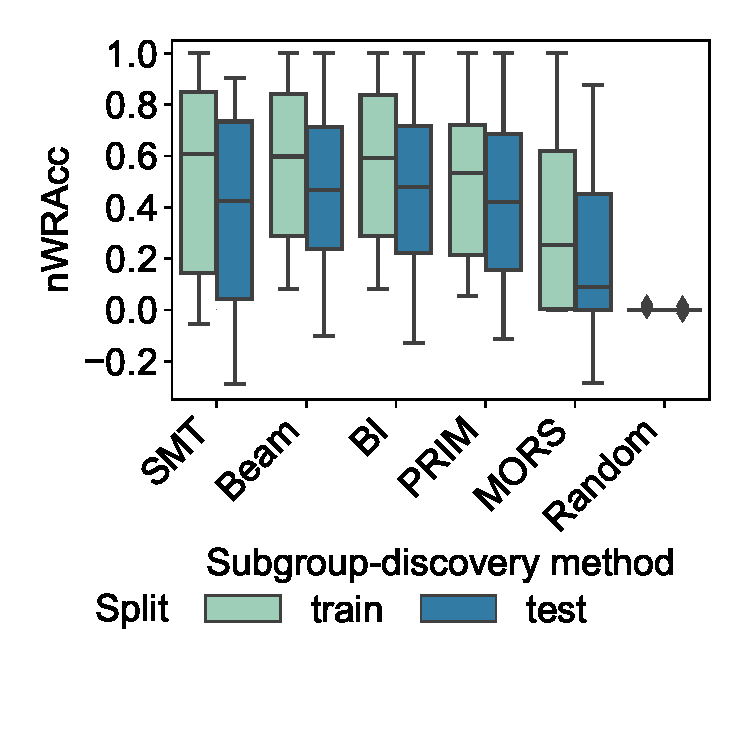
\includegraphics[width=\textwidth, trim=15 55 15 15, clip]{plots/csd-unconstrained-nwracc-all-datasets.pdf}
		\caption{All 27 datasets.}
		\label{fig:csd:unconstrained-nwracc-all-datasets}
	\end{subfigure}
	\hfill
	\begin{subfigure}[t]{0.48\textwidth}
		\centering
		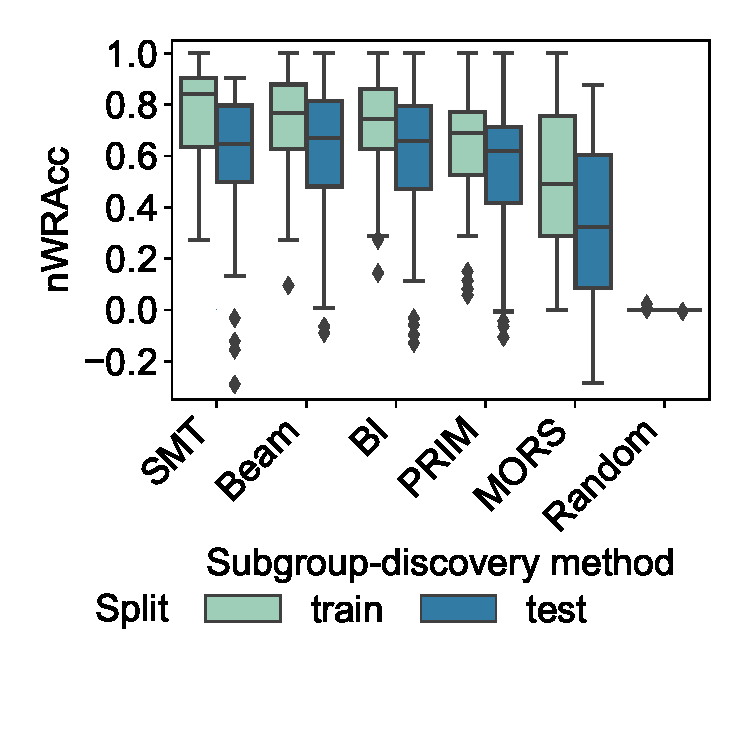
\includegraphics[width=\textwidth, trim=15 55 15 15, clip]{plots/csd-unconstrained-nwracc-no-timeout-datasets.pdf}
		\caption{17 datasets without \emph{SMT} timeouts.}
		\label{fig:csd:unconstrained-nwracc-no-timeout-datasets}
	\end{subfigure}
	\caption{
		Distribution of subgroup quality over datasets and cross-validation folds, by subgroup-discovery method.
		Results from the unconstrained experimental scenario.
	}
	\label{fig:csd:unconstrained-nwracc}
\end{figure}

\paragraph{Subgroup quality}

Figure~\ref{fig:csd:unconstrained-nwracc-all-datasets} compares subgroup quality for the six subgroup-discovery methods.
On the training set, the two heuristic search methods \emph{Beam} and \emph{BI} have roughly the same median nWRAcc as the solver-based search method \emph{SMT}.
In particular, the heuristics are even better than \emph{SMT} on some datasets but worse on others.
The former can happen when \emph{SMT} yields suboptimal solutions due to timeouts, as we analyze later (cf.~Section~\ref{sec:csd:evaluation:timeouts}).
However, even if we limit our analysis to the 17 datasets without \emph{SMT} timeouts, \emph{Beam} and \emph{BI} are still remarkably close to the optimum quality (cf.~Figure~\ref{fig:csd:unconstrained-nwracc-no-timeout-datasets}).
This result is not specific to \emph{SMT} but also affects any other exhaustive search method.
On the test set, \emph{Beam} and \emph{BI} are even better than \emph{SMT} on median, also excluding timeout datasets, since their training-test nWRAcc difference is smaller.
This result indicates that \emph{Beam} and \emph{BI} are less susceptible to overfitting, so their solutions generalize better.
In detail, the average difference between training-set nWRAcc and test-set nWRAcc is 0.122 for \emph{SMT}, 0.101 for \emph{BI}, 0.095 for \emph{Beam}, 0.094 for \emph{MORS}, 0.068 for \emph{PRIM}, and 0.001 for \emph{Random}.

The heuristic search method \emph{PRIM} yields worse subgroup quality than \emph{Beam} and \emph{BI}.
Although it follows an iterative subgroup-refinement procedure like the latter two methods, its refinement options are more limited.
In particular, \emph{PRIM} always has to remove a fixed fraction~$\alpha$ of data objects from the subgroup (cf.~Algorithm~\ref{al:csd:prim}), while \emph{Beam} and \emph{BI} can remove more or less.
Finally, all three heuristic search methods clearly beat the two baselines \emph{MORS} and \emph{Random}.
While \emph{Random} mostly yields the same quality as not restricting the subgroup at all, i.e., an nWRAcc of~0, \emph{MORS} is considerably above~0 and thus a suitable baseline for future studies comparing subgroup-discovery methods.

\begin{table}[t]
	\centering
	\caption{
		Aggregated runtime over datasets and cross-validation folds, by subgroup-discovery method.
		Results from the unconstrained experimental scenario.
	}
	\begin{subtable}{\textwidth}
		\centering
		\caption{
			All 27 datasets.
		}
		\begin{tabular}{lrrrrrr}
			\toprule
			Aggregate & BI & Beam & MORS & PRIM & Random & SMT \\
			\midrule
			Mean & 34.95~s & 30.47~s & 0.01~s & 1.26~s & 0.91~s & 849.02~s \\
			Standard deviation & 103.61~s & 85.69~s & 0.00~s & 1.51~s & 0.95~s & 929.60~s \\
			Median & 2.60~s & 2.95~s & 0.01~s & 0.66~s & 0.51~s & 254.21~s \\
			\bottomrule
		\end{tabular}
		\label{tab:csd:unconstrained-runtime-all-datasets}
	\end{subtable}
	\\ \vspace{\baselineskip}
	\begin{subtable}{\textwidth}
		\centering
		\caption{
			17 datasets without \emph{SMT} timeouts.
		}
		\begin{tabular}{lrrrrrr}
			\toprule
			Aggregate & BI & Beam & MORS & PRIM & Random & SMT \\
			\midrule
			Mean & 12.40~s & 11.77~s & 0.01~s & 1.29~s & 0.82~s & 168.13~s \\
			Standard deviation & 21.17~s & 20.47~s & 0.00~s & 1.62~s & 0.89~s & 243.11~s \\
			Median & 2.60~s & 2.95~s & 0.01~s & 0.80~s & 0.56~s & 57.23~s \\
			\bottomrule
		\end{tabular}
		\label{tab:csd:unconstrained-runtime-no-timeout-datasets}
	\end{subtable}
	\label{tab:csd:unconstrained-runtime}
\end{table}

\paragraph{Runtime}

Table~\ref{tab:csd:unconstrained-runtime} summarizes the runtimes of the subgroup-discovery methods.
On average, \emph{SMT} is an order of magnitude slower than \emph{Beam} and \emph{BI}, which are an order of magnitude slower than \emph{PRIM} and the baseline \emph{Random}.
The baseline \emph{MORS} runs in negligible time and thus is a good tool for instantaneously obtaining a lower bound on subgroup quality.
Taking subgroup quality into consideration, the heuristic search methods offer a good quality in a short time.
Among the three heuristics, \emph{PRIM} is the fastest but yields the lowest subgroup quality, so users should decide which runtime is acceptable.

For \emph{SMT}, the runtime not only comprises optimization but also formulating the optimization problem.
Since the latter depends on the dataset size, e.g., involves $O(m)$ constraints with length $O(n)$ each to define the subgroup-membership variables~$b_i$ (cf.~Equation~\ref{eq:csd:smt-constraint-subgroup-membership}), the preparation time can become considerable for large datasets.
In our experiments, formulating the \emph{SMT} problem took 45~s on average, with a maximum of 379~s.
This average preparation time is already greater than the average total runtime of the heuristics.

\begin{table}[t]
	\centering
	\caption{
		Spearman correlation between runtime and metrics for dataset size,
		over datasets and cross-validation folds, by subgroup-discovery method.
		Results from the unconstrained experimental scenario, using the 17 datasets without \emph{SMT} timeouts.
	}
	\begin{tabular}{lrrrr}
		\toprule
		Method & $\Sigma n^u$ & $m \cdot n$ & $m$ & $n$ \\
		\midrule
		BI & 0.95 & 0.51 & 0.32 & 0.67 \\
		Beam & 0.96 & 0.49 & 0.30 & 0.66 \\
		MORS & 0.27 & 0.57 & 0.51 & 0.26 \\
		PRIM & 0.84 & 0.56 & 0.29 & 0.76 \\
		Random & 0.58 & 0.69 & 0.42 & 0.77 \\
		SMT & 0.39 & 0.73 & 0.70 & 0.23 \\
		\bottomrule
	\end{tabular}
	\label{tab:csd:unconstrained-runtime-correlation}
\end{table}

To determine which factors influence runtime, we analyze the Spearman correlation between runtime and four simple metrics for dataset size.
In particular, Table~\ref{tab:csd:unconstrained-runtime-correlation} considers the number of data objects~$m$, the number of features~$n$, the product of these two quantities~$m \cdot n$, and the number of unique values per feature summed over the features~$\Sigma n^u$.
For the three heuristic search methods, the latter metric shows a high correlation to runtime, while \emph{SMT} exhibits the highest runtime correlation to~$m \cdot n$.

\subsection{Solver Timeouts}
\label{sec:csd:evaluation:timeouts}

In this section, we evaluate the impact of solver timeouts for \emph{SMT} search.

\begin{figure}[t]
	\centering
	\begin{subfigure}[t]{0.48\textwidth}
		\centering
		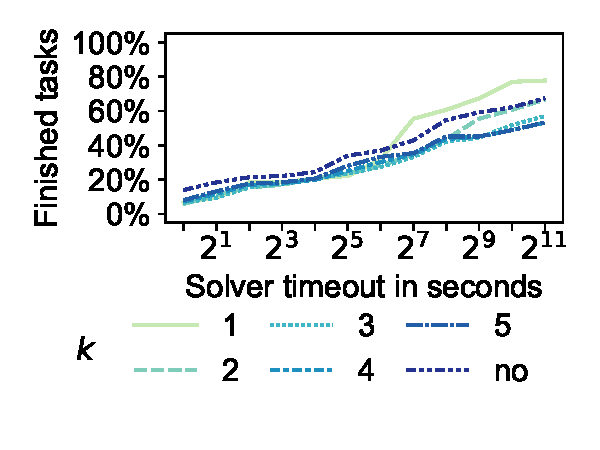
\includegraphics[width=\textwidth, trim=15 25 15 10, clip]{plots/csd-timeouts-finished-tasks.pdf}
		\caption{
			Frequency of finished \emph{SMT} tasks over datasets and cross-validation folds, by feature cardinality~$k$.
		}
		\label{fig:csd:timeouts-finished-tasks}
	\end{subfigure}
	\hfill
	\begin{subfigure}[t]{0.48\textwidth}
		\centering
		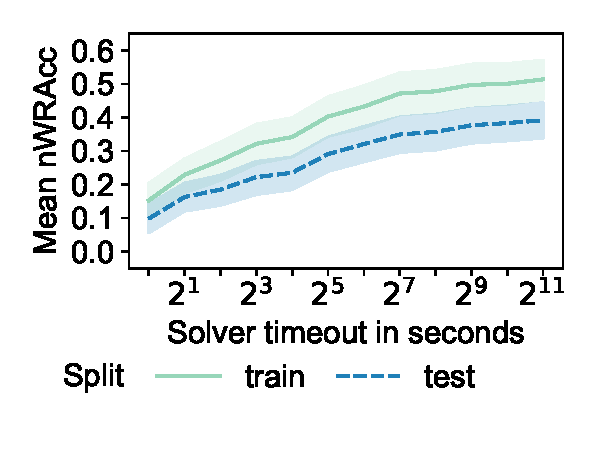
\includegraphics[width=\textwidth, trim=15 25 15 10, clip]{plots/csd-timeouts-nwracc.pdf}
		\caption{
			Mean subgroup quality, with 95\% confidence intervals based on datasets and cross-validation folds.
			Results from the unconstrained experimental scenario.
		}
		\label{fig:csd:timeouts-nwracc}
	\end{subfigure}
	\caption{
		Impact of solver timeouts for \emph{SMT} as the subgroup-discovery method.
		Results from the search for original subgroups.
	}
	\label{fig:csd:timeouts}
\end{figure}

\paragraph{Finished tasks}

Figure~\ref{fig:csd:timeouts-finished-tasks} displays how many of the \emph{SMT} optimization tasks for original subgroups finished within the evaluated solver timeouts.
Besides the unconstrained tasks, we also consider different feature-cardinality thresholds, though the overall trend is the same.
In particular, the number of finished tasks only increases slowly over time, and some tasks take orders of magnitude longer than others.
E.g., in the unconstrained experimental scenario, 21.5\% of the \emph{SMT} tasks finished within 4~s, 24.4\% within 16~s, 37.0\% within 64~s, 54.8\% within 256~s, and 62.2\% within 1024~s.
For the maximum setting of 2048~s, 67.4\% of the \emph{SMT} tasks finished, and 17 out of 27 datasets did not encounter timeouts (cf.~Table~\ref{tab:csd:datasets}).

\paragraph{Subgroup quality}

Figure~\ref{fig:csd:timeouts-nwracc} visualizes the subgroup quality over solver timeouts for unconstrained \emph{SMT} search.
This plot uses the quality of the optimal solution for finished tasks and of the currently best solution for unfinished tasks.
As for the number of finished tasks (cf.~Figure~\ref{fig:csd:timeouts-finished-tasks}), the largest gains occur in the first minute.
E.g., the mean test-set nWRAcc over datasets and cross-validation folds is 0.10 for 1~s, 0.19 for 4~s, 0.24 for 16~s, 0.32 for 64~s, and 0.39 for the maximum solver timeout of 2024~s.
The main cause for this trend is that many tasks finish relatively early (cf.~Figure~\ref{fig:csd:timeouts-finished-tasks}), and finished tasks cannot improve their quality for higher solver timeouts.
In contrast, if we only consider the tasks where the solver did not finish even within the maximum solver timeout, the quality increase of the currently best solution over time is marginal.

Further, even \emph{SMT} with a timeout does not compare favorably to fast heuristic search methods.
E.g., with a solver timeout of 64~s, corresponding to an average overall runtime of 88~s, \emph{SMT} achieves a mean training-set nWRAcc of 0.43, compared to 0.56 for \emph{Beam} with an average runtime of 30~s (cf.~Table~\ref{tab:csd:unconstrained-runtime-all-datasets}).
Finally, setting a lower solver timeout decreases overfitting, i.e., the difference between training-set nWRAcc and test-set nWRAcc increases over time (cf.~Figure~\ref{fig:csd:timeouts-nwracc}).
However, since the test-set nWRAcc still increases with the timeout, choosing lower timeouts does not help quality-wise.

\subsection{Feature-Cardinality Constraints}
\label{sec:csd:evaluation:cardinality}

In this section, we compare all subgroup-discovery methods in the experimental scenario with feature-cardinality constraints.
\emph{SMT} uses its default solver timeout of 2048~s.

\begin{figure}[t]
	\centering
	\begin{subfigure}[t]{0.48\textwidth}
		\centering
		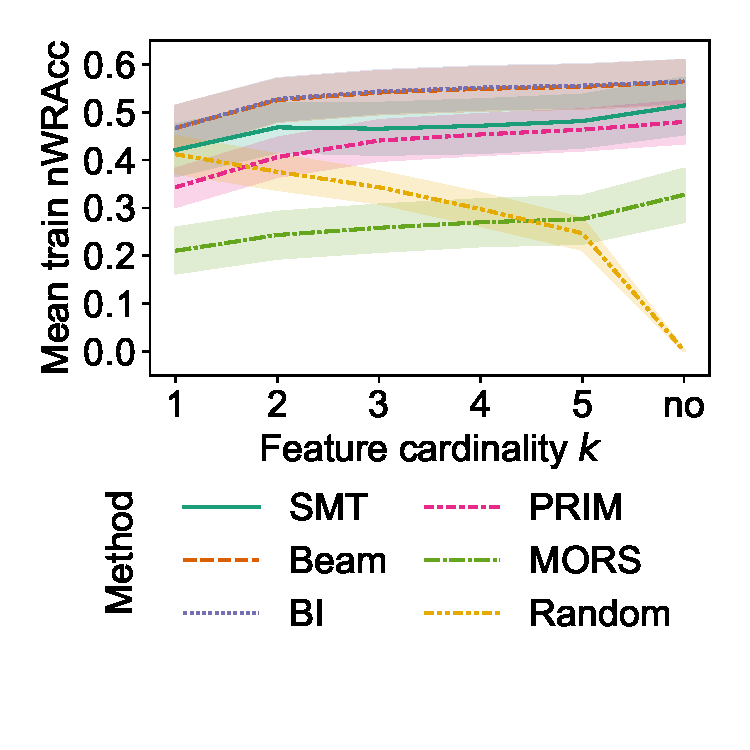
\includegraphics[width=\textwidth, trim=15 55 15 15, clip]{plots/csd-cardinality-train-nwracc-all-datasets.pdf}
		\caption{All 27 datasets, training set.}
		\label{fig:csd:cardinality-train-nwracc-all-datasets}
	\end{subfigure}
	\hfill
	\begin{subfigure}[t]{0.48\textwidth}
		\centering
		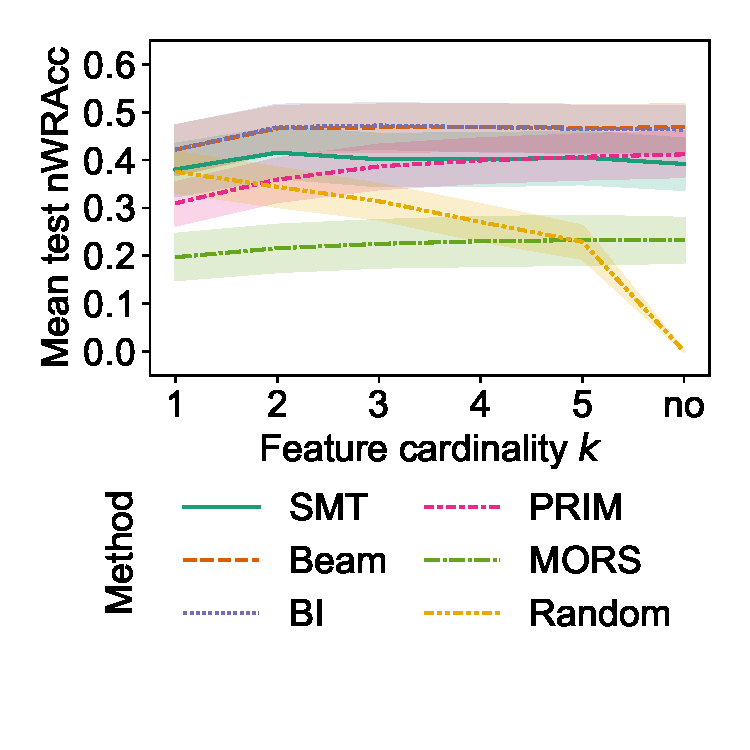
\includegraphics[width=\textwidth, trim=15 55 15 15, clip]{plots/csd-cardinality-test-nwracc-all-datasets.pdf}
		\caption{All 27 datasets, test set.}
		\label{fig:csd:cardinality-test-nwracc-all-datasets}
	\end{subfigure}
	\\
	\begin{subfigure}[t]{0.48\textwidth}
		\centering
		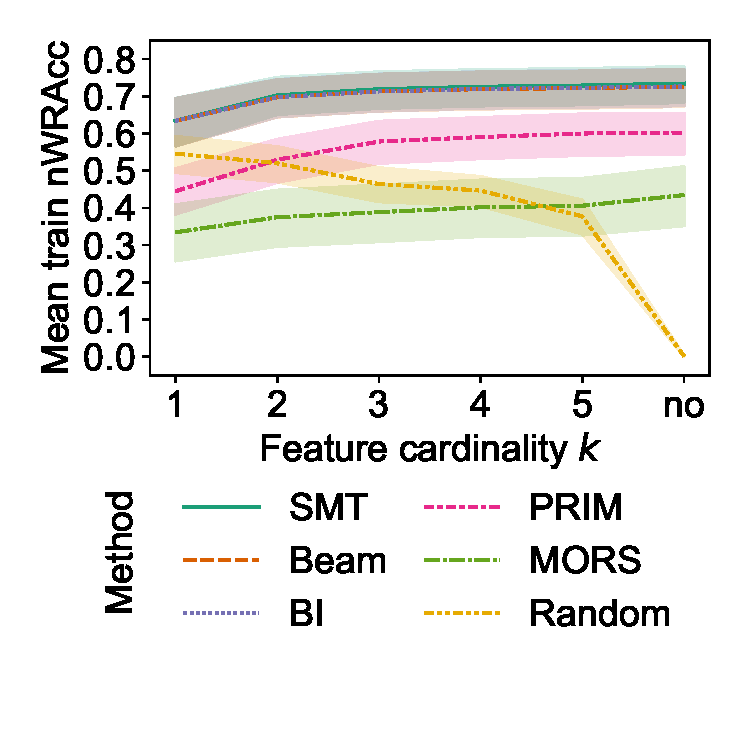
\includegraphics[width=\textwidth, trim=15 55 15 15, clip]{plots/csd-cardinality-train-nwracc-no-timeout-datasets.pdf}
		\caption{13 datasets without \emph{SMT} timeouts, training set.}
		\label{fig:csd:cardinality-train-nwracc-no-timeout-datasets}
	\end{subfigure}
	\hfill
	\begin{subfigure}[t]{0.48\textwidth}
		\centering
		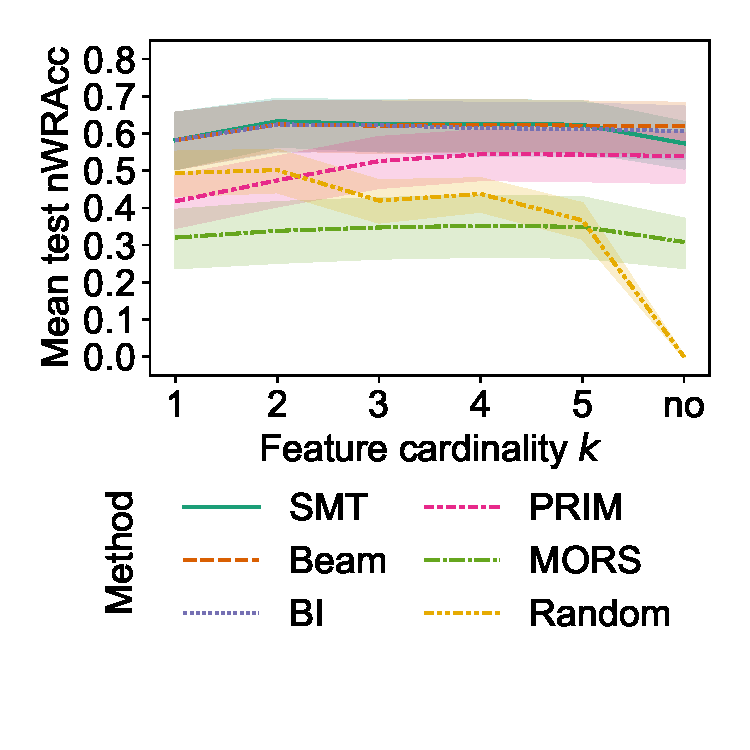
\includegraphics[width=\textwidth, trim=15 55 15 15, clip]{plots/csd-cardinality-test-nwracc-no-timeout-datasets.pdf}
		\caption{13 datasets without \emph{SMT} timeouts, test set.}
		\label{fig:csd:cardinality-test-nwracc-no-timeout-datasets}
	\end{subfigure}
	\caption{
		Mean subgroup quality, with 95\% confidence intervals based on datasets and cross-validation folds, by subgroup-discovery method and feature cardinality~$k$.
		Results from the search for original subgroups.
	}
	\label{fig:csd:cardinality-nwracc}
\end{figure}

\paragraph{Subgroup quality}

Figure~\ref{fig:csd:cardinality-nwracc} displays the mean subgroup quality, averaging over datasets and cross-validation folds, for different values of the feature-cardinality threshold~$k$.
For most subgroup-discovery methods, mean training-set nWRAcc (cf.~Figure~\ref{fig:csd:cardinality-train-nwracc-all-datasets}) increases with~$k$, though the marginal utility decreases.
In particular, even with $k=1$, the mean nWRAcc is already clearly above 50\% of the nWRAcc achieved with all features.
Further, the quality increase between $k=1$ and $k=2$ is usually the largest.
On the test set (cf.~Figure~\ref{fig:csd:cardinality-test-nwracc-all-datasets}), the benefit of setting a larger~$k$ is even smaller.
E.g., the mean test-set nWRAcc of \emph{Beam}, \emph{BI}, and \emph{SMT} barely improves beyond $k=2$.
These results indicate that sparse subgroup descriptions already yield a high subgroup quality.
The baseline \emph{Random} even improves subgroup quality with lower~$k$ due to its design (cf.~Algorithm~\ref{al:csd:random-search}):
\emph{Random} samples bounds independently for each feature.
The more features are used in the subgroup description, the smaller the expected number of data objects in the subgroup becomes.
However, the number of subgroup members is one factor in WRAcc (cf.~Equation~\ref{eq:csd:wracc}).

Figures~\ref{fig:csd:cardinality-train-nwracc-all-datasets} and~\ref{fig:csd:cardinality-test-nwracc-all-datasets} also reveal that the heuristic search methods \emph{Beam} and \emph{BI} still yield higher average subgroup quality than the solver-based search \emph{SMT} due to timeouts, for any feature-cardinality setting.
Even excluding the datasets with \emph{SMT} timeouts (cf.~Figures~\ref{fig:csd:cardinality-train-nwracc-no-timeout-datasets} and~\ref{fig:csd:cardinality-test-nwracc-no-timeout-datasets}), these two heuristics yield nearly the same average subgroup quality as \emph{SMT} for constrained~$k$ and have an advantage on the test set with unconstrained~$k$.
The heuristic \emph{PRIM} exhibits a larger increase of subgroup quality over~$k$ than \emph{Beam} and \emph{BI}, thereby narrowing the quality gap to the latter.
The baseline \emph{MORS} displays the least effect of~$k$ on mean test-set nWRAcc, showing very stable subgroup quality.

Finally, the results indicate that limiting~$k$ reduces overfitting.
For example, \emph{Beam} has a mean training-test nWRAcc difference of 0.095 without limiting~$k$, 0.073 for $k=3$, and 0.045 for $k=1$.
The increasing tendency to overfit with larger~$k$ explains why mean training-set nWRAcc increases more than mean test-set nWRAcc over~$k$ in Figure~\ref{fig:csd:cardinality-nwracc}.
\emph{PRIM} shows the smallest increase of overfitting over~$k$, \emph{MORS} and \emph{SMT} the largest.

\begin{table}[t]
	\centering
	\caption{
		Mean runtime over datasets and cross-validation folds, by subgroup-discovery method and feature cardinality~$k$.
		Results from the search for original subgroups.
	}
	\begin{tabular}{lrrrrrr}
		\toprule
		$k$ & BI & Beam & MORS & PRIM & Random & SMT \\
		\midrule
		1 & 7.81~s & 6.81~s & 0.01~s & 0.08~s & 0.63~s & 648.16~s \\
		2 & 11.74~s & 10.06~s & 0.01~s & 0.17~s & 0.64~s & 911.28~s \\
		3 & 14.20~s & 12.78~s & 0.01~s & 0.26~s & 0.65~s & 1091.75~s \\
		4 & 16.68~s & 14.65~s & 0.01~s & 0.35~s & 0.66~s & 1113.40~s \\
		5 & 18.66~s & 16.12~s & 0.01~s & 0.46~s & 0.66~s & 1117.39~s \\
		no & 34.95~s & 30.47~s & 0.01~s & 1.26~s & 0.91~s & 849.02~s \\
		\bottomrule
	\end{tabular}
	\label{tab:csd:cardinality-runtime}
\end{table}

\paragraph{Runtime}

As Table~\ref{tab:csd:cardinality-runtime} displays, the heuristic search methods \emph{Beam}, \emph{BI}, and \emph{PRIM} become faster the smaller~$k$ is.
The baseline \emph{Random} shows a similar trend, though less prominent, while \emph{MORS} yields results instantaneously in any case.
In contrast, the picture for the solver-based search method \emph{SMT} is less clear.
While its average runtime clearly increases from $k=1$ till $k=3$, it roughly remains constant for $k \in \{4, 5\}$ and even decreases without a feature-cardinality constraint, only remaining higher than for $k = 1$.

\subsection{Alternative Subgroup Descriptions}
\label{sec:csd:evaluation:alternatives}

In this section, we analyze alternative subgroup descriptions for \emph{Beam} and \emph{SMT}.
Both employ a feature cardinality of~$k=3$.
\emph{SMT} uses its default solver timeout of 2048~s.

\begin{figure}[t]
	\centering
	\begin{subfigure}[t]{0.48\textwidth}
		\centering
		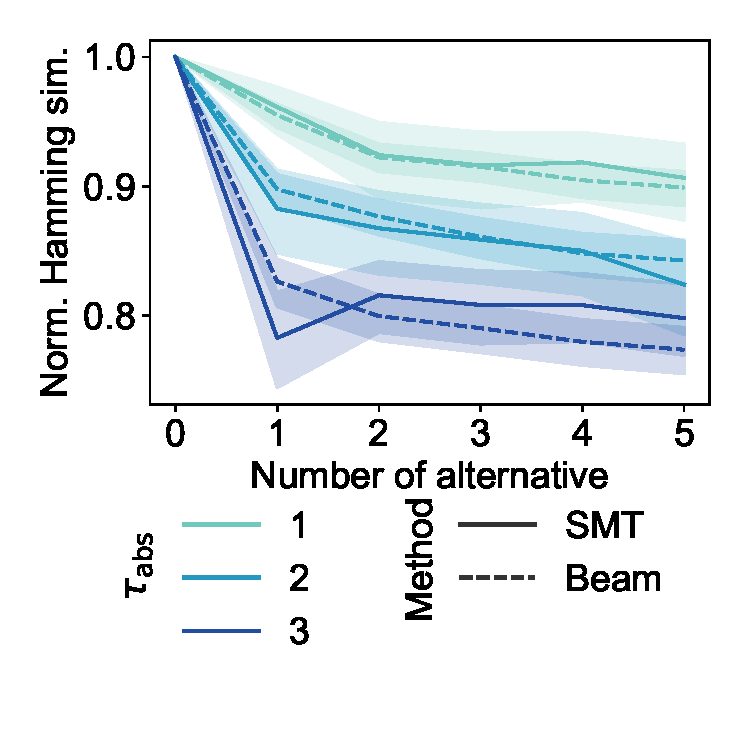
\includegraphics[width=\textwidth, trim=15 50 15 15, clip]{plots/csd-alternatives-hamming.pdf}
		\caption{Normalized Hamming similarity.}
		\label{fig:csd:alternatives-hamming}
	\end{subfigure}
	\hfill
	\begin{subfigure}[t]{0.48\textwidth}
		\centering
		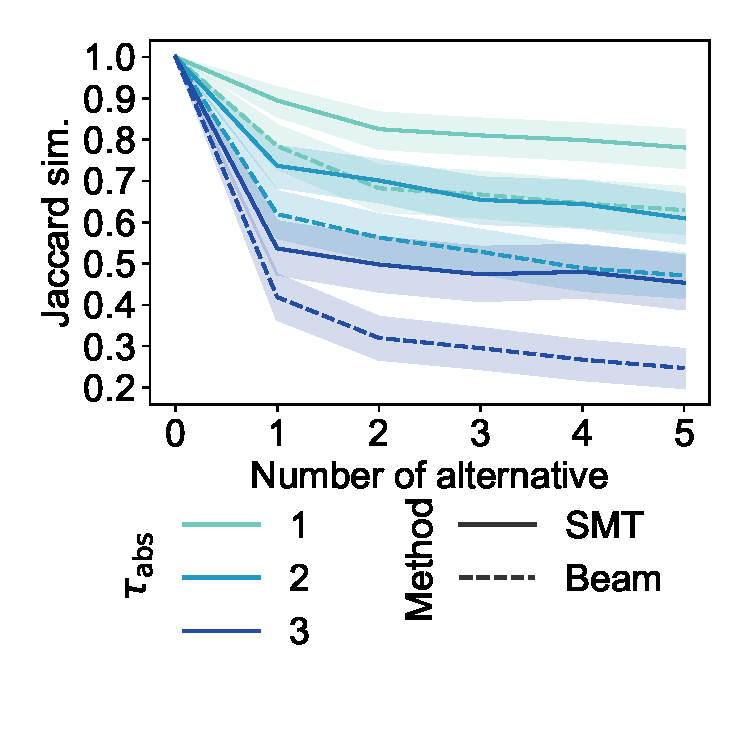
\includegraphics[width=\textwidth, trim=15 50 15 15, clip]{plots/csd-alternatives-jaccard.pdf}
		\caption{Jaccard similarity.}
		\label{fig:csd:alternatives-jaccard}
	\end{subfigure}
	\caption{
		Mean subgroup similarity of alternative subgroup descriptions to the original subgroup, with 95\% confidence intervals based on datasets and cross-validation folds, by subgroup-discovery method, number of alternative, and dissimilarity threshold~$\tau_{\text{abs}}$.
	}
	\label{fig:csd:alternatives-similarity}
\end{figure}

\paragraph{Subgroup similarity}

Figure~\ref{fig:csd:alternatives-similarity} visualizes the average similarity between the original subgroups and those induced by alternative subgroup descriptions.
As expected, the subgroup-membership similarity decreases the more alternatives one desires and the more the selected features in subgroup descriptions should differ.
Further, the decrease is strongest from the original subgroup, i.e., the zeroth alternative, to the first alternative but smaller beyond.
This observation indicates that one may find several alternative subgroup descriptions of comparable similarity to the original.

These trends hold for both similarity measures, i.e., the normalized Hamming similarity we optimize (cf.~Equation~\ref{eq:csd:hamming-general} and Figure~\ref{fig:csd:alternatives-hamming}) as well as the Jaccard similarity (cf.~Equation~\ref{eq:csd:jaccard} and Figure~\ref{fig:csd:alternatives-jaccard}).
The latter yields lower similarity values than the former since it ignores data objects that are not contained in either of the two compared subgroups.
Further, the observed trends exist for the solver-based search method \emph{SMT} as well as the heuristic search method \emph{Beam}.
\emph{SMT} yields clearly more similar subgroups than \emph{Beam} for the Jaccard similarity, while the normalized Hamming similarity does not show a clear winner.

\begin{figure}[t]
	\centering
	\begin{subfigure}[t]{0.48\textwidth}
		\centering
		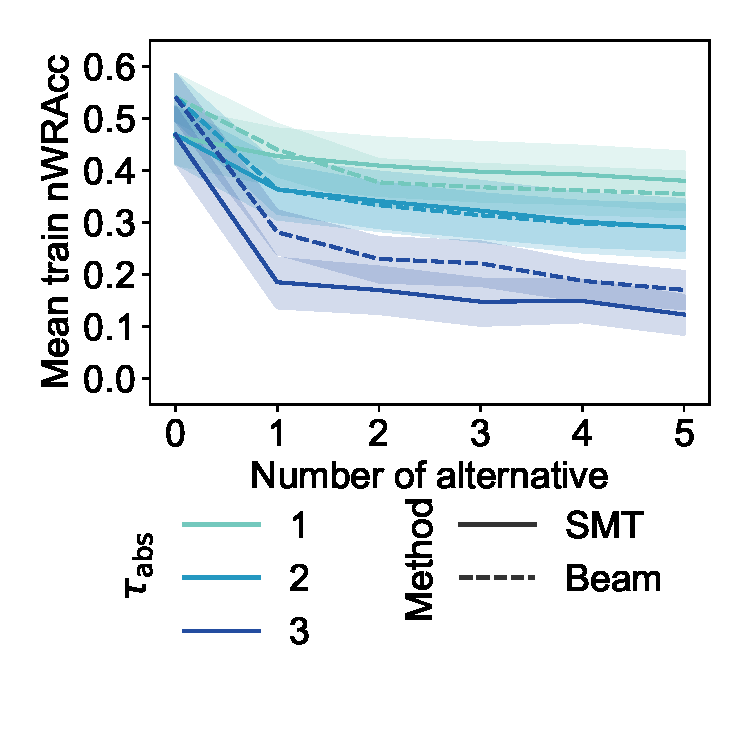
\includegraphics[width=\textwidth, trim=15 50 15 15, clip]{plots/csd-alternatives-train-nwracc.pdf}
		\caption{Training set.}
		\label{fig:csd:alternatives-train-nwracc}
	\end{subfigure}
	\hfill
	\begin{subfigure}[t]{0.48\textwidth}
		\centering
		\includegraphics[width=\textwidth, trim=15 50 15 15, clip]{plots/csd-alternatives-test-nwracc.pdf}
		\caption{Test set.}
		\label{fig:csd:alternatives-test-nwracc}
	\end{subfigure}
	\caption{
		Mean subgroup quality of alternative subgroup descriptions, with 95\% confidence intervals based on datasets and cross-validation folds, by subgroup-discovery method, number of alternative, and dissimilarity threshold~$\tau_{\text{abs}}$.
	}
	\label{fig:csd:alternatives-nwracc}
\end{figure}

\paragraph{Subgroup quality}

The average subgroup quality of alternative subgroup descriptions (cf.~Figure~\ref{fig:csd:alternatives-nwracc}) shows similar trends as subgroup similarity (cf.~Figure~\ref{fig:csd:alternatives-similarity}) and the quality of alternative feature sets in our previous chapter (cf.~Figure~\ref{fig:afs:impact-num-alternatives-tau-quality}).
In particular, quality decreases over the dissimilarity threshold~$\tau_{\text{abs}}$ and over the number of alternatives~$a$, with the largest decrease to the first alternative.
For the highest dissimilarity threshold~$\tau_{\text{abs}} = 3$, \emph{Beam} consistently yields higher average quality than \emph{SMT} for the original subgroup and each alternative.
In contrast, the other two values of the dissimilarity threshold do not clearly favor either method.
The observed trends on the test set (cf.~Figure~\ref{fig:csd:alternatives-test-nwracc}) are very similar to those on the training set (cf.~Figure~\ref{fig:csd:alternatives-train-nwracc}).
For both subgroup-discovery methods, overfitting, as measured by the training-test difference in nWRAcc, is lower for the alternative subgroup descriptions than for the original subgroups.
This phenomenon may result from the alternatives not directly optimizing subgroup quality.

\begin{table}[t]
	\centering
	\caption{
		Mean runtime over datasets and cross-validation folds, by subgroup-discovery method, dissimilarity threshold~$\tau_{\text{abs}}$, and number of alternative.
		Results from the search for alternative subgroup descriptions.
	}
	\begin{tabular}{llrrrrrr}
		\toprule
		\multirow{2}{*}{Method} & \multirow{2}{*}{$\tau_{\text{abs}}$} & \multicolumn{6}{c}{Number of alternative} \\
		\cmidrule(lr){3-8}
		& &  0 & 1 & 2 & 3 & 4 & 5 \\
		\midrule
		\multirow[t]{3}{*}{Beam} & 1 & 12.8~s & 8.0~s & 7.6~s & 7.3~s & 7.3~s & 7.3~s \\
		& 2 & 12.8~s & 7.7~s & 7.4~s & 7.2~s & 7.0~s & 6.8~s \\
		& 3 & 12.8~s & 5.8~s & 5.1~s & 4.7~s & 4.1~s & 3.5~s \\
		\multirow[t]{3}{*}{SMT} & 1 & 1091.7~s & 166.0~s & 221.5~s & 239.6~s & 258.1~s & 277.9~s \\
		& 2 & 1105.2~s & 377.5~s & 463.5~s & 537.5~s & 599.4~s & 658.3~s \\
		& 3 & 1107.4~s & 869.1~s & 670.8~s & 597.6~s & 588.1~s & 557.6~s \\
		\bottomrule
	\end{tabular}
	\label{tab:csd:alteratives-runtime}
\end{table}

\paragraph{Runtime}

Table~\ref{tab:csd:alteratives-runtime} displays the average runtime for searching original subgroups and alternative subgroup descriptions.
The search for alternatives is faster for both analyzed search methods, i.e., \emph{Beam} and \emph{SMT}.
As for the original subgroups, \emph{Beam} search for alternatives is one to two orders of magnitude faster than the solver-based \emph{SMT} search.
For \emph{Beam}, runtime tends to decrease over the number of alternatives, while \emph{SMT} shows a less clear behavior.
In particular, its runtime increases over alternatives for~$\tau_{\text{abs}} \in \{1, 2\}$, i.e., settings that allow reusing features from previous subgroup descriptions.
In contrast, runtime decreases over alternatives for $\tau_{\text{abs}} = k = 3$, which forbids reusing any feature selected before.
Finally, the number of \emph{SMT} tasks finished within the solver timeout shows trends corresponding to the runtime.
In particular, there are more finished tasks when searching for alternative subgroup descriptions than for original subgroups.

\subsection{Summary}
\label{sec:csd:evaluation:summary}

\paragraph{Unconstrained subgroup discovery (cf.~Section~\ref{sec:csd:evaluation:unconstrained})}

We recommend using heuristic search methods rather than solver-based search.
In particular, \emph{Beam} and \emph{BI} were an order of magnitude faster than \emph{SMT} and still yielded higher test-set subgroup quality since they overfit less.
The latter result not only impedes \emph{SMT} but other exhaustive search methods as well.
\emph{PRIM} was faster than \emph{Beam} and \emph{BI} but yielded lower subgroup quality.
Our novel baseline \emph{MORS} provided instantaneous, non-trivial lower bounds for subgroup quality.

\paragraph{Solver timeouts (cf.~Section~\ref{sec:csd:evaluation:timeouts})}

Setting larger solver timeouts showed a decreasing marginal utility regarding the number of finished \emph{SMT} tasks and subgroup quality, i.e., most gains occurred within the first dozens of seconds.
About half the \emph{SMT} tasks that finished at all finished in under a minute.
However, the average subgroup quality with this solver timeout was lower than for heuristic search methods with even lower runtime.

\paragraph{Feature-cardinality constraints (cf.~Section~\ref{sec:csd:evaluation:cardinality})}

Using more features in subgroup descriptions showed a decreasing marginal utility regarding subgroup quality.
For \emph{Beam}, \emph{BI}, and \emph{SMT}, test-set subgroup quality was already close to the unconstrained scenario at $k=2$, while \emph{PRIM} benefited more from larger~$k$.
A smaller~$k$ made the heuristic search methods faster and generally reduced overfitting.
\emph{MORS} showed stable test-set subgroup quality regarding~$k$, while \emph{Random} even increased subgroup quality with smaller~$k$.

\paragraph{Alternative subgroup descriptions (cf.~Section~\ref{sec:csd:evaluation:alternatives})}

The heuristic \emph{Beam} was one to two orders of magnitude faster than solver-based \emph{SMT} when searching for alternative subgroup descriptions, while both search methods found alternatives faster than original subgroups.
The quality and similarity of alternatives strongly depended on the number of alternatives~$a$ and the dissimilarity threshold~$\tau_{\text{abs}}$.
The difference in quality and similarity between the original and the first alternative was higher than among the first few alternatives.


\chapter{Conclusions}
\label{sec:conclusions}

This dissertation focused on making feature selection more user-centric with the help of constraints.
In particular, we tackled two research gaps that have not received sufficient attention in the literature before (cf.~Section~\ref{sec:introduction:research-gaps}):
integrating domain knowledge and finding alternative solutions.
We addressed these two issues by formulating constraints on the selected feature sets.
In particular, we made the following contributions:

In Chapter~\ref{sec:syn}, we formally introduced the optimization problem of constrained feature selection.
Our definition is orthogonal to the user's choice of a feature-selection method, as it retains the method's notion of feature-set quality.
We proposed using an SMT solver for optimization, which supports a wide range of constraint types.
Additionally, we systematically evaluated the impact of constraints on feature selection.
Our comprehensive study generated constraints with varying characteristics and quantified the feature-selection results with multiple evaluation metrics.
Section~\ref{sec:syn:evaluation:summary} summarizes central results.

In Chapter~\ref{sec:ms}, we applied constrained feature selection in a domain-specific case study.
We worked with materials scientists to express preferences and scientific hypotheses as constraints.
Section~\ref{sec:ms:evaluation:summary} summarizes central results.

In Chapter~\ref{sec:afs}, we introduced the optimization problem of alternative feature selection.
We formalized alternatives via 0-1 integer linear constraints, which are independent of the feature-selection method and allow users to control the number and dissimilarity of alternatives.
Additionally, we discussed how to combine these constraints with different categories of existing feature-selection methods.
For a simple notion of feature-set quality, we showed that the optimization problem is $\mathcal{NP}$-hard but a constant-factor approximation exists, for which we proposed corresponding heuristics.
Finally, we conducted extensive experiments with five feature-selection methods, five search methods for alternatives, and different values of the two user parameters.
Section~\ref{sec:afs:evaluation:summary} summarizes central results.

In Chapter~\ref{sec:csd}, we analyzed feature-selection-related constraints in subgroup discovery.
We formalized subgroup discovery as an SMT optimization problem, focusing on two constraint types:
limiting the number of features used in subgroups and searching for alternative subgroup descriptions.
Further, we proved $\mathcal{NP}$-hardness of these two constrained optimization problems.
We also showed how to integrate these constraint types into existing heuristic search methods for subgroup discovery.
Finally, we evaluated heuristic and solver-based search in four experimental scenarios:
unconstrained subgroup discovery, our two constraint types, and solver timeouts.
Section~\ref{sec:csd:evaluation:summary} summarizes central results.

For all contributions, we made our code and experimental data available online (cf.~Section~\ref{sec:introduction:materials}).
Finally, we will discuss directions for future work in the next chapter.

\chapter{Future Work}
\label{sec:future-work}

In this section, we outline potential directions for future research.

\paragraph{Integrating more conventional methods}

Our notions of constraints and alternatives are orthogonal to conventional methods for feature selection and subgroup discovery.
While we successfully showed how to integrate constraints, we could naturally only evaluate a combination with a few existing methods.
Thus, there is room for integrating constraints into further methods.
E.g., we implemented only one procedure to find alternatives for wrapper feature selection (cf.~Section~\ref{sec:afs:approach:objectives:black-box}) and did not adapt embedded feature selection, which does not admit a generic solution procedure (cf.~Section~\ref{sec:afs:approach:objectives:embedding}).

\paragraph{Further problem encodings and solvers}

In each chapter, we focused on one problem encoding and solver, i.e., SMT via \emph{Z3} (cf.~Chapters~\ref{sec:syn}, \ref{sec:ms}, and~\ref{sec:csd}) or 0-1 integer linear programming via \emph{SCIP} (cf.~Chapter~\ref{sec:afs}).
One could analyze further problem encodings, e.g., using \textsc{MaxSAT}, and compare additional solvers.
For subgroup discovery, we assumed numerical features and a binary target (cf.~Section~\ref{sec:fundamentals:subgroup-discovery:problem}).
To support more datasets, one could adapt the encoding to multi-valued categorical features and continuous targets.

\paragraph{Heuristic search}

For alternative feature selection, we developed heuristic search methods and showed membership in the complexity class~$\mathcal{APX}$ for univariate feature qualities (cf.~Equation~\ref{eq:fs:univariate-filter}) under certain conditions (cf.~Proposition~\ref{prop:afs:approximation-apx}).
One could attempt to tighten the quality bounds we derived or show membership in a narrower complexity class.
Additionally, one could develop heuristic search methods for other notions of feature-set quality.
For subgroup discovery, we described how to integrate feature-cardinality constraints and alternative subgroup descriptions into heuristic search methods (cf.~Sections~\ref{sec:csd:approach:cardinality:heuristics} and~\ref{sec:csd:approach:alternatives:heuristics}).
However, proving quality-approximation guarantees is still open.

\paragraph{Further definitions of alternatives}

One could vary the definition of alternatives, e.g., the set-dissimilarity measure (cf.~Equations~\ref{eq:afs:dice} and~\ref{eq:csd:constraint-dissimilarity}).
However, one should ensure that the corresponding search method supports the desired change, e.g., requiring linearity for integer linear programming or antimonotonicity for specific heuristic search methods. 
For simultaneous alternatives, there are different options to aggregate the quality of feature sets (cf.~Section~\ref{sec:afs:approach:constraints:multiple}).
For subgroup discovery, one could analyze solver-based search for alternatives in the sense of covering different data objects, as used in related work (cf.~Section~\ref{sec:related-work:alternatives:subgroup-discovery}), rather than covering the same data objects differently, as we did.

\paragraph{Soft constraints}

We only employed hard constraints, i.e., all constraints had to be satisfied.
As we observed, this can result in reduced feature-set quality or even an infeasible solution.
With soft constraints, users could attach individual penalties to each constraint violation and thereby specify how to trade off constraint satisfaction against feature-set quality.
Alternatively, one could treat constraint satisfaction as another objective besides feature-set quality and apply multi-objective optimization.
The set of Pareto-optimal solutions may allow users to compare different constraint-quality trade-offs.

\paragraph{Time complexity}

Our various $\mathcal{NP}$-hardness results made assumptions on the problem definition, e.g., parametrization of the search for alternatives.
One could attempt to obtain further hardness results for other scenarios.
For alternative feature selection, our analysis (cf.~Section~\ref{sec:afs:approach:complexity:univariate}) assumed univariate feature qualities (cf.~Equation~\ref{eq:fs:univariate-filter}).
Results for other feature-selection methods may differ.
In the univariate scenario, we obtained $\mathcal{NP}$-hardness for min-aggregation with feature-set overlap (cf.~Proposition~\ref{prop:afs:complexity-no-partitioning-min-constrained-k}) and polynomial runtime for sum-aggregation without overlap (cf.~Proposition~\ref{prop:afs:complexity-partitioning-sum}).
However, an analysis of sum-aggregation with overlap remains open.
For subgroup discovery, we showed $\mathcal{NP}$-hardness of finding alternative subgroup descriptions (cf.~Propositions~\ref{prop:csd:complexity-perfect-alternatives-np-perfect-subgroup}, \ref{prop:csd:complexity-perfect-alternatives-np-imperfect-subgroup}, and~\ref{prop:csd:complexity-alternatives-np}) but focused on scenarios without feature-set overlap.
Additionally, our proofs assumed a feature-cardinality constraint (cf.~Definition~\ref{def:csd:feature-cardinality-constraint}) when searching alternative subgroup descriptions.
One could examine scenarios without this constraint type.

\paragraph{Case studies}

While we conducted a case study for constrained feature selection (cf.~Chapters~\ref{sec:ms}), our other experiments used generic benchmark datasets and quantitative evaluation metrics (cf.~Chapters~\ref{sec:syn}, \ref{sec:afs}, and~\ref{sec:csd}).
In particular, we focused on uncovering general trends rather than dataset-specific insights.
Since all the methods introduced in this dissertation are domain-independent, one could also employ them in domain-specific case studies and interpret the corresponding results qualitatively, i.e., from the domain perspective.

\paragraph{User-friendly systems}

We made all our generally applicable methods available for reuse via Python packages.
Also, we implemented specific evaluation routines to create figures and tables.
However, users may prefer an application with a graphical user interface to run analyses and inspect results themselves.
In particular, an interactive tool could ease trying out different constraints or varying the parameters for alternatives.
For constrained feature selection, one would need to design a user-friendly way to formulate constraints.
For all methods, runtime is an essential concern for interactivity.
This point could be addressed with solver timeouts, fast heuristics, and runtime estimates shown to users.

\paragraph{Constrained feature engineering}

In this dissertation, we took the datasets as-is, i.e., assuming all features were engineered already.
However, one could integrate constraints into feature engineering as well, steering the creation of new features rather than the selection of existing ones.
For example, one could desire only to engineer features with specific characteristics or limit the combination of certain feature-engineering operators.


\printbibliography

%%% Back matter %%%

\appendix

\chapter{Appendix}
\label{sec:appendix}

In this chapter, we provide supplementary materials for Chapter~\ref{sec:afs} (cf.~Section~\ref{sec:appendix:afs}) and Chapter~\ref{sec:csd} (cf.~Section~\ref{sec:appendix:csd}).

\section{\nameref*{sec:afs}}
\label{sec:appendix:afs}

In this section, we provide supplementary materials for Chapter~\ref{sec:afs}.
Section~\ref{sec:appendix:afs:univariate-complete-optimization-problem} provides complete definitions of the alternative-feature-selection problem (cf.~Section~\ref{sec:afs:approach:constraints}) for the univariate objective (cf.~Equation~\ref{eq:fs:univariate-filter}).
Section~\ref{sec:appendix:afs:proofs} contains proofs for the complexity analysis with the univariate objective (cf.~Section~\ref{sec:afs:approach:complexity:univariate}).

\subsection{Complete Optimization Problems for the Univariate Objective}
\label{sec:appendix:afs:univariate-complete-optimization-problem}

In this section, we provide complete specifications of the alternative-feature-selection problem for sequential and simultaneous search as a 0-1 integer linear problem.
In particular, we combine all relevant definitions and equations from Section~\ref{sec:afs:approach}.
We use the objective of univariate filter feature selection (cf.~Equation~\ref{eq:fs:univariate-filter}).
The corresponding feature qualities $q(\cdot)$ are constants in the optimization problem.
Further, we use the Dice dissimilarity (cf.~Equations~\ref{eq:afs:dice} and~\ref{eq:afs:dice-rearranged-equal-size}) to measure feature-set dissimilarity for alternatives.
The dissimilarity threshold~$\tau \in [0,1]$ is a user-defined constant.
Finally, we assume fixed, user-defined feature-set sizes~$k \in \mathbb{N}$.

\paragraph{Sequential-search problem}

In the sequential case (cf.~Definition~\ref{def:afs:alternative-feature-selection-sequential} and Equation~\ref{eq:afs:afs-sequential}), only one feature set~$F_s$ is variable in the optimization problem, while the existing feature sets $F_{\bar{s}} \in \mathbb{F}$ with their selection vectors $\bar{s}$ are constants.
%
\begin{equation}
	\begin{aligned}
		\max_s &\quad & Q_{\text{uni}}(s,X,y) &= \sum_{j=1}^{n} q(X_{\cdot{}j},y) \cdot s_j \\
		\text{subject to:} &\quad \forall F_{\bar{s}} \in \mathbb{F}: & \sum_{j=1}^n s_j \cdot \bar{s}_j &\leq (1 - \tau) \cdot k \\
		&\quad & \sum_{j=1}^n s_j &= k \\
		&\quad & s &\in \{0,1\}^n
	\end{aligned}
	\label{eq:afs:afs-sequential-complete}
\end{equation}
%
\paragraph{Simultaneous-search problem}

In the simultaneous case (cf.~Definition~\ref{def:afs:alternative-feature-selection-simultaneous} and Equation~\ref{eq:afs:afs-simultaneous}), all feature sets are variable.
$a \in \mathbb{N}_0$ denotes the number of alternatives, which corresponds to the number of feature sets minus one.
Next, we introduce auxiliary variables to linearize products between decision variables (cf.~Equation~\ref{eq:afs:product-linear}).
Finally, we use sum-aggregation (cf.~Equation~\ref{eq:afs:afs-simultaneous-sum-objective}) over alternatives in the objective here.
%
\begin{equation}
	\begin{aligned}
		\max_{s^{(0)}, \dots, s^{(a)}} &\quad & \sum_l Q_{\text{uni}}(s^{(l)},X,y) &= \sum_l \sum_j q(X_{\cdot{}j},y) \cdot s^{(l)}_j\\
		\text{subject to:} &\quad \forall l_1~\forall l_2: & \sum_j t^{(l_1,l_2)}_j &\leq (1 - \tau) \cdot k \\
		&\quad \forall l_1~\forall l_2~\forall j: & t^{(l_1,l_2)}_j &\leq s^{(l_1)}_j \\
		&\quad \forall l_1~\forall l_2~\forall j: & t^{(l_1,l_2)}_j &\leq s^{(l_2)}_j \\
		&\quad \forall l_1~\forall l_2~\forall j: & 1 + t^{(l_1,l_2)}_j &\geq s^{(l_1)}_j + s^{(l_2)}_j \\
		&\quad \forall l: & \sum_j s^{(l)}_j &= k \\
		&\quad \forall l: & s^{(l)} &\in \{0,1\}^n \\
		&\quad \forall l_1~\forall l_2: & t^{(l_1,l_2)} &\in \{0,1\}^n \\
		\text{with indices:} &\quad & l &\in \{0, \dots, a\} \\
		&\quad & l_1 &\in \{1, \dots, a\} \\
		&\quad & l_2 &\in \{0, \dots, l_1-1\} \\
		&\quad & j &\in \{1, \dots, n\}
	\end{aligned}
	\label{eq:afs:afs-simultaneous-complete}
\end{equation}

\subsection{Proofs}
\label{sec:appendix:afs:proofs}

In this section, we provide proofs for propositions from Section~\ref{sec:afs:approach:complexity:univariate}, i.e., complexity results for alternative feature selection with univariate feature qualities.

\subsubsection{Proof of Proposition~\ref{prop:afs:complexity-incomplete-partitioning-min-constrained-k}}
\label{sec:appendix:afs:proofs:complexity-incomplete-partitioning-min-constrained-k}

\begin{proof}
	Let~$I$ be an arbitrary problem instance of the simultaneous-search problem with min-aggregation, univariate feature qualities, a complete-partitioning scenario, and a fixed feature-set size~$k$ (cf.~Proposition~\ref{prop:afs:complexity-partitioning-min-constrained-k}).
	We add a new feature~$f'$ to~$I$ and keep the parameters $a$, $k$, and $\tau$ as before, obtaining an instance~$I'$ of the incomplete-partitioning scenario since one feature will not be selected.
	We set the quality~$q'$ of~$f'$ to be lower than all other feature qualities in~$I$.
	Since the univariate objective monotonically increases in the selected feature qualities, selecting feature~$f'$ in a solution of~$I'$ does not have any benefit since~$f'$ would replace a feature with higher quality.
	If~$f'$ is not selected, this solution of~$I'$ also solves~$I$.
	However, if the qualities of the alternatives are not equal, $f'$ might still be chosen in a set that does not have the minimum quality of all sets since only the latter determines the objective value (cf.~Example~\ref{ex:afs:min-aggregation}).
	In that case, we replace $f'$ with the remaining unselected feature; the objective value remains the same, and the solution becomes valid for~$I$.
	Thus, in any case, we can easily transform a solution for~$I'$ to a solution for~$I$.
	
	Overall, an algorithm for incomplete partitioning can solve arbitrary complete-partitioning instances with negligible computational overhead.
	Thus, a polynomial-time algorithm for incomplete partitioning could also solve complete partitioning polynomially.
	However, the latter problem is $\mathcal{NP}$-complete (cf.~Proposition~\ref{prop:afs:complexity-partitioning-min-constrained-k}), so incomplete partitioning has to be $\mathcal{NP}$-hard.
	Since checking a solution for incomplete partitioning needs only polynomial time, we obtain membership in $\mathcal{NP}$ and thereby $\mathcal{NP}$-completeness.
\end{proof}

\subsubsection{Proof of Proposition~\ref{prop:afs:complexity-no-partitioning-min-constrained-k}}
\label{sec:appendix:afs:proofs:complexity-no-partitioning-min-constrained-k}

\begin{proof}
	Let~$I$ be an arbitrary problem instance of the simultaneous-search problem with min-aggregation, univariate feature qualities, a complete-partitioning scenario, the Dice dissimilarity (cf.~Equation~\ref{eq:afs:dice}) as~$d(\cdot)$, and a fixed feature-set size~$k$ (cf.~Proposition~\ref{prop:afs:complexity-partitioning-min-constrained-k}).
	We create a new problem instance~$I'$ by adding a new feature~$f'$ and increasing the feature-set size to $k' = k + 1$.
	Further, we set $\tau' = (k' - 1) / k'$, thereby allowing an overlap of at most one feature between feature sets.
	Also, we choose~$f'$ to have a considerably higher quality~$q'$ than all other features.
	Our goal is to force the selection of~$f'$ in all feature sets, no matter which other features are selected.
	One possible choice is $q' = \sum_{j=1}^n q_j + \varepsilon$ for a small $\varepsilon \in \mathbb{R}_{> 0}$
	This quality~$q'$ of~$f'$ is higher than of any feature set not containing it.
	Thus, a solution for~$I'$ contains~$f'$ in each feature set, while the remaining features are part of exactly one feature set.
	Hence, we can remove~$f'$ to get feature sets of size~$k = k' - 1$ that constitute an optimal solution for the original problem instance~$I$.
	
	This transformation shows how an algorithm for problem instances with $\tau < 1$ can help solve arbitrary problem instances with $\tau = 1$.
	Given the $\mathcal{NP}$-completeness of the latter problem (cf.~Proposition~\ref{prop:afs:complexity-partitioning-min-constrained-k}), we obtain $\mathcal{NP}$-hardness of the former.
\end{proof}
%
One can transfer this reduction from $\tau' = (k' - 1) / k'$ to all other $\tau > 0$.
In particular, for a given~$k$, there is only a finite number of $\tau$ values leading to different set overlaps, e.g., $\tau = \{0, 1/k, \dots, (k - 1) / k, 1\}$ for the Dice dissimilarity.
The proof for the highest overlap except~$\tau=0$ requires creating an instance $I'$ with $\tau'= 1/k$ from an instance with $\tau = 1$.
For this purpose, $k^2 - k$ features need to be added since $\tau' = k / k' = k / (k + k^2 -k) = 1/k$.
I.e., $k$ out of $k' = k^2$ features need to form a complete partitioning, while the remaining $k^2 - k$~features occur in each feature set and will be removed after solving~$I'$.
The number of features to be added is polynomial in~$k$ and thereby also polynomial in~$n$.

\subsubsection{Proof of Proposition~\ref{prop:afs:complexity-partitioning-sum}}
\label{sec:appendix:afs:proofs:complexity-partitioning-sum}

\begin{proof}
	We discuss the simultaneous-search problem (cf.~Definition~\ref{def:afs:alternative-feature-selection-simultaneous}) with sum-aggregation (cf.~Equation~\ref{eq:afs:afs-simultaneous-sum-objective}) first.
	We leverage the monotonicity of the univariate objective with sum-aggregation.
	In particular, this objective cannot decrease when selecting features of higher quality.
	Thus, we order all features decreasingly by their quality, which yields the complexity of~$O(n \cdot \log n)$.
	Next, we pick features in this order without replacement and assign them to sets until we have the user-defined number of alternatives with the user-defined feature-set sizes.
	Apart from observing cardinality constraints, the actual assignment of the selected features to sets does not matter quality-wise since swapping features between sets does not change the summed objective.
	Thus, one can fill the feature sets in an arbitrary order.
	Each assignment runs in $O(1)$, e.g., using arrays to store feature-set membership, yielding $O(n)$ for all features.
	Without cardinality constraints, only the number of alternatives needs to be satisfied.
	Further, if all features need to be selected, i.e., for a complete partitioning, one need not sort the features.
	Finally, if only a small fraction of features needs to be selected, one might slightly improve complexity to $O(k \cdot n)$ by iteratively picking the maximum instead of sorting all qualities.

	For the sequential-search problem (cf.~Definition~\ref{def:afs:alternative-feature-selection-sequential}), we conduct the same quality-sorting procedure.
	In contrast to the simultaneous-search problem, the actual assignment of features to sets matters since the sets have an explicit order.
	In particular, each alternative should get the remaining highest-quality features until its user-defined size is reached.
	The complexity is still dominated by sorting and therefore~$O(n \cdot \log n)$.
\end{proof}

\section{\nameref*{sec:csd}}
\label{sec:appendix:csd}

In this section, we supplement Chapter~\ref{sec:csd}.
Section~\ref{sec:appendix:csd:milp-encoding} describes how to encode constrained subgroup discovery as a mixed integer linear program, complementing Section~\ref{sec:csd:approach:smt}.
Section~\ref{sec:appendix:csd:proofs} contains proofs for complexity propositions from Section~\ref{sec:csd:approach}.

\subsection{Encoding via Mixed Integer Linear Programming (MILP)}
\label{sec:appendix:csd:milp-encoding}

We start from the SMT formulation and introduce additional variables and constraints to linearize certain logical expressions.

\paragraph{Unconstrained subgroup discovery}

We keep all decision variables from the corresponding SMT formulation (cf.~Equation~\ref{eq:csd:smt-problem-unconstrained-complete}):
the binary variables~$b_i$ for subgroup membership and the real-valued bound variables~$\mathit{lb}_j$ and~$\mathit{ub}_j$.
The bound constraints (cf.~Equation~\ref{eq:csd:smt-constraint-bounds-monotonic}) remain unchanged as well.
Further, we retain the optimization objective, which already is linear in~$b_i$ (cf.~Equations~\ref{eq:csd:smt-wracc} and~\ref{eq:csd:smt-constraint-m-as-sum}).
However, we need to linearize the logical AND ($\land$) operators in the definition of subgroup membership~$b_i$ (cf.~Equation~\ref{eq:csd:smt-constraint-subgroup-membership}) by introducing auxiliary variables and further constraints.
In particular, we supplement the variables~$b \in \{0, 1\}^m$ by $b^{\text{lb}} \in \{0, 1\}^{m \times n}$ and $b^{\text{ub}} \in \{0, 1\}^{m \times n}$.
These new binary variables indicate whether a particular data object satisfies the lower or upper bound for a particular feature.
Using linearization techniques for constraint satisfaction and AND operators from~\cite{mosek2022modeling}, we obtain the following set of constraints to replace Equation~\ref{eq:csd:smt-constraint-subgroup-membership}:

\begin{equation}
	\begin{aligned}
		\forall i~\forall j: & & X_{ij} + m_j \cdot b^{\text{lb}}_{ij} &\leq \mathit{lb}_j - \varepsilon_j \\
		\forall i~\forall j: & & \mathit{lb}_j &\leq X_{ij} + M_j \cdot \left(1 - b^{\text{lb}}_{ij} \right) \\
		\forall i~\forall j: & & \mathit{ub}_j + m_j \cdot b^{\text{ub}}_{ij} &\leq X_{ij} - \varepsilon_j \\
		\forall i~\forall j: & & X_{ij} &\leq \mathit{ub}_j + M_j \cdot \left(1 - b^{\text{ub}}_{ij} \right) \\
		\forall i~\forall j: & & b_i &\leq b^{\text{lb}}_{ij} \\
		\forall i~\forall j: & & b_i &\leq b^{\text{ub}}_{ij} \\
		\forall i: & & \sum_{j=1}^{n} \left( b^{\text{lb}}_{ij} + b^{\text{ub}}_{ij} \right) &\leq b_i + 2n - 1 \\
		\text{with indices:} & & i &\in \{1, \dots, m\} \\
		& & j &\in \{1, \dots, n\}
	\end{aligned}
	\label{eq:csd:milp-constraint-subgroup-membership}
\end{equation}
%
The first two inequalities ensure that $b^{\text{lb}}_{ij} = 1$ if and only if $\mathit{lb}_j \leq X_{ij}$.
The following two inequalities relate~$b^{\text{ub}}_{ij}$ to $X_{ij} \leq \mathit{ub}_j$.
The values~$\varepsilon_j \in \mathbb{R}_{> 0}$ are small constants that turn strict inequalities into non-strict ones since a MILP solver may only support the latter.
One possible choice is to sort all unique feature values and take the minimum difference between two consecutive values in that order.
The values~$M_j \in \mathbb{R}_{> 0}$ and $m_j \in \mathbb{R}_{< 0}$ are large positive and negative constants, respectively.
They help to connect real-valued and binary-valued expressions, compensating for the latter's smaller range.
One choice for~$M_j$ is a value larger than the difference between the feature's minimum and maximum:
%
\begin{equation}
	\begin{aligned}
		\forall j \in \{1, \dots, n\} & & M_j &:= 2 \cdot \left( \max_{i \in \{1, \dots, m\}} X_{ij} - \min_{i \in \{1, \dots, m\}} X_{ij} \right) \\
		\forall j \in \{1, \dots, n\} & & m_j &:= 2 \cdot \left( \min_{i \in \{1, \dots, m\}} X_{ij} - \max_{i \in \{1, \dots, m\}} X_{ij} \right) \\
	\end{aligned}
	\label{eq:csd:milp-big-m}
\end{equation}
%
In particular, the difference between the subgroup's bounds and arbitrary feature values must be smaller than $M_j$ and larger than $m_j$, unless the bounds are placed outside the feature's value range.
Since the latter does not improve the subgroup's quality in any case, we prevent it with additional constraints on the bound variables~$\mathit{lb}_j$ and~$\mathit{ub}_j$:
%
\begin{equation}
	\begin{aligned}
		\forall j \in \{1, \dots, n\} & & \min_{i \in \{1, \dots, m\}} X_{ij} &\leq \mathit{lb}_j &\leq \max_{i \in \{1, \dots, m\}} X_{ij} \\
		\forall j \in \{1, \dots, n\} & & \min_{i \in \{1, \dots, m\}} X_{ij} &\leq \mathit{ub}_j &\leq \max_{i \in \{1, \dots, m\}} X_{ij} \\
	\end{aligned}
	\label{eq:csd:milp-constraint-bounds-in-range}
\end{equation}
%
Finally, the last three inequalities in Equation~\ref{eq:csd:milp-constraint-subgroup-membership} tie $b^{\text{lb}}_{ij}$ and $b^{\text{ub}}_{ij}$ to $b_i$ and linearize the logical AND ($\land$) operators from Equation~\ref{eq:csd:smt-constraint-subgroup-membership}.
In particular, these constraints ensure that a data object is a member of the subgroup, i.e., $b_i = 1$, if and only if all feature values of the data object observe the bounds, i.e., all corresponding $b^{\text{lb}}_{ij} = 1$ and $b^{\text{ub}}_{ij} = 1$.

\paragraph{Feature-cardinality constraints}

The feature-cardinality constraint of the SMT formulation (cf.~Equation~\ref{eq:csd:smt-constraint-feature-cardinalty}) already is a linear expression in the feature-selection variables~$s_j$.
However, the constraints defining~$s_j$ (cf.~Equation~\ref{eq:csd:smt-constraint-feature-selection}) contain a logical OR ($\lor$) operator and comparison ($<$) expressions.
We linearize these constraints as follows:
%
\begin{equation}
	\begin{aligned}
		\forall i~\forall j: & & 1 - b^{\text{lb}}_{ij} &\leq s^{\text{lb}}_j \\
		\forall i~\forall j: & & 1 - b^{\text{ub}}_{ij} &\leq s^{\text{ub}}_j \\
		\forall j: & & s^{\text{lb}}_j &\leq s_j \\
		\forall j: & & s^{\text{ub}}_j &\leq s_j \\
		\forall j: & & s_j &\leq 2m - \sum_{i=1}^{m} \left( b^{\text{lb}}_{ij} + b^{\text{ub}}_{ij} \right) \\
		\text{with indices:} & & i &\in \{1, \dots, m\} \\
		& & j &\in \{1, \dots, n\}
	\end{aligned}
	\label{eq:csd:milp-constraint-feature-selection}
\end{equation}
%
The first four inequalities ensure that a feature is selected, i.e., $s_j = 1$, if any data object's feature value lies outside the subgroup's bounds, i.e., any $b^{\text{lb}}_{ij} = 0$ or $b^{\text{ub}}_{ij} = 0$.
The last inequality covers the other direction of the logical equivalence:
If a feature is selected, then at least one data object's feature value lies outside the subgroup's bounds.

\paragraph{Alternative subgroup descriptions}

The objective function for alternative subgroup descriptions in the SMT formulation (cf.~Equation~\ref{eq:csd:smt-hamming}) is already linear.
We only need to replace the logical negation ($\lnot$) operator:
%
\begin{equation}
	\text{sim}_{\text{nHamm}}(b^{(a)}, b^{(0)}) = \frac{1}{m} \cdot \Big( \sum\limits_{\substack{i \in \{1, \dots, m\} \\ b_i^{(0)} = 1}} b_i^{(a)} + \sum\limits_{\substack{i \in \{1, \dots, m\} \\ b_i^{(0)} = 0}} \left( 1 - b_i^{(a)} \right) \Big)
	\label{eq:csd:mip-hamming}
\end{equation}
%
The same replacement also applies to the dissimilarity constraints (cf.~Equation~\ref{eq:csd:smt-constraint-dissimilarity}):
%
\begin{equation}
	\forall l \in \{0, \dots, a-1\}:~ \text{dis}_{\text{des}}(s^{(a)}, s^{(l)}) = \sum_{\substack{j \in \{1, \dots, n\} \\ s^{(l)}_j = 1}} \left(1 - s^{(a)}_j \right) \geq \min \left( \tau_{\text{abs}},~k^{(l)} \right)
	\label{eq:csd:mip-constraint-dissimilarity}
\end{equation}
%
Otherwise, this expression already is linear as well.

\paragraph{Implementation}

Our published code (cf.~Section~\ref{sec:introduction:materials}) contains a MILP implementation for unconstrained and feature-cardinality-constrained subgroup discovery.
We use the package \emph{OR-Tools}~\cite{perron2022or-tools} with \emph{SCIP}~\cite{bestuzheva2021scip} as the optimizer.
However, in preliminary experiments, this implementation was (on average) slower than the SMT implementation or yielded worse subgroup quality in the same runtime.
Further, it sometimes finished considerably after the prescribed timeout or ran out of memory after consuming dozens of gigabytes.
Thus, we stuck to the SMT implementation for our main experiments (cf.~Section~\ref{sec:csd:experimental-design:methods}).

\subsection{Proofs}
\label{sec:appendix:csd:proofs}

In this section, we provide proofs for propositions from Section~\ref{sec:csd:approach}, particularly for the complexity results for subgroup discovery with a feature-cardinality constraint and for searching alternative subgroup descriptions.

\subsubsection{Proof of Proposition~\ref{prop:csd:complexity-cardinality-np-perfect-subgroup}}
\label{sec:appendix:csd:proofs:complexity-cardinality-np-perfect-subgroup}

\begin{proof}
	Let~$I$ be an arbitrary instance of the decision problem \textsc{Set Covering}~\cite{karp1972reducibility}.
	$I$ consists of a set of elements~$E = \{e_1, \dots, e_m\}$, a set of sets~$\mathbb{S} = \{S_1,  \dots, S_n\}$ with $E = \bigcup_{S \in \mathbb{S}} S$, and a cardinality threshold~$k \in \mathbb{N}$.
	\textsc{Set Covering} asks whether a subset $\mathbb{C} \subseteq \mathbb{S}$ exists with $|\mathbb{C}| \leq k$ and $E = \bigcup_{S \in \mathbb{C}} S$, i.e., a subset of~$\mathbb{S}$ which contains (= covers) each element from~$E$ in at least one set and consist of at most $k$~sets.
	
	We transform~$I$ into an instance~$I'$ of the perfect-subgroup-discovery problem (cf.~Definition~\ref{def:csd:perfect-subgroup-discovery}) with a feature-cardinality constraint (cf.~Definition~\ref{def:csd:feature-cardinality-constraint}).
	To this end, we define a binary dataset~$X \in \{0, 1\}^{(m + 1) \times n}$, prediction target~$y \in \{0, 1\}^{m+1}$, and retain the number of sets~$k \in \mathbb{N}$ as feature cardinality~$k$.
	In particular, data objects represent elements from~$E$, and features represent sets from~$\mathbb{S}$.
	$X_{ij}$ denotes $e_i \in S_j$, i.e., membership of Element~$i$ in Set~$j$.
	The additional index $i = m + 1$ represents a \emph{dummy element} that is not part of any set, so all its feature values are set to~0.
	Further, we define the prediction target~$y \in \{0, 1\}^{m+1}$ as $y_{m+1} = 1$ and $y_i = 0$ for all other indices $i \in \{1, \dots, m\}$.
	This prediction target represents whether an element should \emph{not} be covered by the set of sets~$\mathbb{C} \subseteq \mathbb{S}$.
	In particular, all elements from~$E$ should be covered but not the new dummy element.
	This `inverted' definition of the prediction target stems from the different nature of set covers and subgroup descriptions:
	Set covers include elements from selected sets, with the empty cover $\mathbb{C} = \emptyset$ containing no elements.
	There is a logical OR ($\lor$) respectively set union over the selected sets.
	In contrast, subgroup descriptions exclude data objects based on bounds for their selected features, with the unrestricted subgroup containing all data objects.
	There is a logical AND ($\land$) over the features' bounds.
	
	A perfect subgroup (cf.~Definition~\ref{def:csd:perfect-subgroup}) exactly replicates the prediction target~$y$ as subgroup membership.
	Here, it only contains the data object representing the dummy element but no data objects representing elements from~$E$.
	As all feature values of this dummy data object are~0, the subgroup description only consists of the bounds $\mathit{lb}_j = \mathit{ub}_j = 0$ for selected features and $\mathit{lb}_j = 0 < 1 = \mathit{ub}_j$ for unselected features.
	Therefore, the data objects described by the selected features represent elements not contained in any selected set, which only applies to the dummy element.
	Vice versa, all remaining data objects represent elements that are part of at least one selected set, which applies to all elements from~$E$.
	Further, the feature-cardinality constraint (cf.~Definition~\ref{def:csd:feature-cardinality-constraint}) ensures that at most $k$~features are selected, which means that at most $k$~sets are selected.
	Thus, the selected features of a perfect subgroup represent sets forming a valid set cover~$\mathbb{C}$.
	In contrast, if no feature set of the desired size~$k$ can describe a perfect subgroup, then at least one data object with prediction target~$y_i = 0$ has to be a subgroup member.
	Thus, at least one element is not contained in any set forming the set cover, so no valid set cover of size~$k$ exists.
	
	Overall, a solution to the instance~$I'$ of the perfect-subgroup discovery problem (cf.~Definition~\ref{def:csd:perfect-subgroup-discovery}) with a feature-cardinality constraint (cf.~Definition~\ref{def:csd:feature-cardinality-constraint}) also solves the instance~$I$ of \textsc{Set Covering} ~\cite{karp1972reducibility} with negligible computational overhead.
	In particular, an efficient algorithm for the former would also efficiently solve the latter.
	However, since the latter problem is $\mathcal{NP}$-hard~\cite{karp1972reducibility}, the former is as well.
	To be more precise, perfect-subgroup discovery with a feature-cardinality constraint resides in~$\mathcal{NP}$ and therefore is $\mathcal{NP}$-complete.
	In particular, checking a solution induces a polynomial cost of~$O(m \cdot n)$, requiring one pass over the dataset to determine subgroup membership and feature selection.
\end{proof}
%
This proof adapts the proof of \cite{boley2009non} for minimizing the feature cardinality of a given subgroup description.
The latter reduces from the optimization problem \textsc{Minimum Set Cover}, while we use the decision problem \textsc{Set Covering}.
Further, we replace the notion of a given subgroup description~\cite{boley2009non} with the notion of a perfect subgroup and employ lower and upper bounds instead of `feature=value' conditions.
The latter difference is irrelevant for binary datasets, where selected features have $\mathit{lb}_j = \mathit{ub}_j$ and thereby implicitly select a feature value.
The hardness result naturally extends to real-valued datasets.

Note that the hardness reduction does not work for the special case $k=n$.
For \textsc{Set Covering}, this case allows all sets to be selected, which trivially solves the problem.
Vice versa, the unconstrained problem of perfect-subgroup discovery (cf.~Definition~\ref{def:csd:perfect-subgroup-discovery}) admits a polynomial-time solution (cf.~Proposition~\ref{prop:csd:complexity-unconstrained-perfect-subgroup}).

\subsubsection{Proof of Proposition~\ref{prop:csd:complexity-cardinality-np}}
\label{sec:appendix:csd:proofs:complexity-cardinality-np}

\begin{proof}
	Let~$I$ be an arbitrary instance of the perfect-subgroup-discovery problem (cf.~Definition~\ref{def:csd:perfect-subgroup-discovery}) with a feature-cardinality constraint (cf.~Definition~\ref{def:csd:feature-cardinality-constraint}).
	We transform~$I$ into an instance~$I'$ of the subgroup-discovery problem (cf.~Definition~\ref{def:csd:subgroup-discovery}) with the same constraint.
	In particular, we define the objective as optimizing subgroup quality~$Q(\mathit{lb}, \mathit{ub}, X, y)$ rather than searching for a perfect subgroup (cf.~Definition~\ref{def:csd:perfect-subgroup}) that may or may not exist.
	The other inputs of the problem instance ($X$, $y$, and $k$) remain the same.
	
	Based on the assumption we made on~$Q(\mathit{lb}, \mathit{ub}, X, y)$ in Proposition~\ref{prop:csd:complexity-cardinality-np}, the optimal solution for~$I'$ is a perfect subgroup if the latter exists.
	Thus, if the optimal subgroup for~$I'$ is not perfect, then a perfect subgroup does not exist at all.
	Checking whether a subgroup is perfect entails a cost of $O(m \cdot n)$, i.e., computing subgroup membership and checking for false positives and false negatives.
	Overall, an algorithm for subgroup discovery (cf.~Definition~\ref{def:csd:subgroup-discovery}) with a feature-cardinality constraint (cf.~Definition~\ref{def:csd:feature-cardinality-constraint}) solves perfect-subgroup discovery (cf.~Definition~\ref{def:csd:perfect-subgroup-discovery}) with the same constraint with negligible overhead.
	Since the latter problem is $\mathcal{NP}$-complete (cf.~Proposition~\ref{prop:csd:complexity-cardinality-np-perfect-subgroup}) and the former resides in the complexity class $\mathcal{NP}$, the former is $\mathcal{NP}$-complete as well.
\end{proof}
%
Alternatively, one could reduce from the optimization problem \textsc{Maximum Coverage}~\cite{chekuri2004maximum}, similar to the proof for Proposition~\ref{prop:csd:complexity-cardinality-np-perfect-subgroup} (cf.~Section~\ref{sec:appendix:csd:proofs:complexity-cardinality-np-perfect-subgroup}), which reduces from the decision problem \textsc{Set Covering}~\cite{karp1972reducibility}.
In contrast to \textsc{Set Covering}, the $k \in \mathbb{N}$~selected subsets in \textsc{Maximum Coverage} need not cover all elements but should cover as many elements as possible.
In subgroup discovery, the latter objective corresponds to a particular notion of subgroup quality:
maximizing the number of true negatives or minimizing the number of false positives, i.e., excluding as many negative data objects from the subgroup as possible.
This problem is minimal-optimal-recall-subgroup discovery (cf.~Definition~\ref{def:csd:minimal-optimal-recall-subgroup-discovery}).
However, the latter's objective is simpler than WRAcc (cf.~Equation~\ref{eq:csd:wracc}), which we focus on in this dissertation.
Our proof above is more general regarding the notion of subgroup quality but more narrow in the sense that it reduces from a search problem, assuming a particular value of the objective function, instead of an optimization problem.

\subsubsection{Proof of Proposition~\ref{prop:csd:complexity-perfect-alternatives-np-perfect-subgroup}}
\label{sec:appendix:csd:proofs:complexity-perfect-alternatives-np-perfect-subgroup}

\begin{proof}
	Let~$I$ be an arbitrary instance of the perfect-subgroup-discovery problem (cf.~Definition~\ref{def:csd:perfect-subgroup-discovery}) with a feature-cardinality constraint (cf.~Definition~\ref{def:csd:feature-cardinality-constraint}).	
	We transform~$I$ into an instance~$I'$ of the perfect-alternative-subgroup-description-discovery problem (cf.~Definition~\ref{def:csd:perfect-alternative-subgroup-description-discovery}) with the same constraint.
	We retain the feature-cardinality threshold~$k \in \mathbb{N}$ and slightly modify the dataset~$X \in \mathbb{R}^{m \times n}$, as explained later.
	
	Based on the assumptions from Proposition~\ref{prop:csd:complexity-perfect-alternatives-np-perfect-subgroup}, we define the original subgroup for~$I'$ to be perfect (cf.~Definition~\ref{def:csd:perfect-subgroup}), i.e., having subgroup membership $b^{(0)} = y$.
	Also, we choose the dissimilarity threshold~$\tau \in \mathbb{R}_{\geq 0}$ high enough that the alternative subgroup description may not select any features from the original subgroup description.
	E.g., we can choose the deselection dissimilarity (cf.~Equation~\ref{eq:csd:constraint-dissimilarity}) and $\tau_{\text{abs}} = k$.
	We need not even explicitly define the original feature selection since we must not select these features in the alternative anyway.
	For the sake of completeness, we can define dataset~$X' \in \mathbb{R}^{m \times (n+k)}$ of problem instance~$I'$ as dataset~$X \in \mathbb{R}^{m \times n}$ of problem instance~$I$ with $k$ features added that equal the prediction target~$y$.
	Choosing the bounds $\mathit{lb}_j = \mathit{ub}_j = 1$ on any of these extra features produces the desired original subgroup membership $b^{(0)} = y$.
	We further assume that all extra features were selected in the original subgroup description but no actual features from~$X$ were, i.e., $\forall j \in \{1, \dots, n\}:~ s^{(0)}_j = 0$ and $\forall j \in \{n+1, \dots, n+k\}:~ s^{(0)}_j = 1$.
	
	A solution for problem instance~$I'$ also solves~$I$.
	In particular, the perfect alternative subgroup description (cf.~Definition~\ref{def:csd:perfect-alternative}) is a perfect subgroup since it perfectly replicates the original subgroup membership, which is perfect, i.e., $b^{(a)} = b^{(0)} = y$.
	Due to the dissimilarity constraint, the alternative subgroup description only selects features from dataset~$X$, not those newly added to create~$X'$.
	Finally, both~$I$ and~$I'$ use a feature-cardinality constraint with threshold~$k$.
	Thus, if a perfect alternative subgroup description for~$I'$ exists, it also solves~$I$.
	If it does not exist, then there is also no other perfect subgroup for~$I$.
	
	Thus, an efficient algorithm for the perfect-alternative-subgroup-description-discovery problem (cf.~Definition~\ref{def:csd:perfect-alternative-subgroup-description-discovery}) with a feature-cardinality constraint (cf.~Definition~\ref{def:csd:feature-cardinality-constraint}) would also efficiently solve perfect-subgroup discovery (cf.~Definition~\ref{def:csd:perfect-subgroup-discovery}) with the same constraint.
	However, we already established that the latter problem is $\mathcal{NP}$-complete (cf.~Proposition~\ref{prop:csd:complexity-cardinality-np-perfect-subgroup}).
	Further, evaluating a solution for the former problem entails a polynomial cost of $O(m \cdot n)$ for checking constraints regarding bounds, feature cardinality, and dissimilarity, placing the problem in complexity class~$\mathcal{NP}$ and thereby making it $\mathcal{NP}$-complete.
\end{proof}

\subsubsection{Proof of Proposition~\ref{prop:csd:complexity-perfect-alternatives-np-imperfect-subgroup}}
\label{sec:appendix:csd:proofs:complexity-perfect-alternatives-np-imperfect-subgroup}

\begin{proof}
	Let~$I$ be an arbitrary instance of the perfect-alternative-subgroup-description-discovery problem (cf.~Definition~\ref{def:csd:perfect-alternative-subgroup-description-discovery}) with a feature-cardinality constraint (cf.~Definition~\ref{def:csd:feature-cardinality-constraint}) and a perfect original subgroup (cf.~Definition~\ref{def:csd:perfect-subgroup}).
	We transform~$I$ into an instance~$I'$ of the same problem but with an imperfect original subgroup.
	In particular, we retain all problem inputs as-is except defining dataset~$X' \in \mathbb{R}^{(m + 1) \times n}$ of~$I'$ as dataset~$X \in \mathbb{R}^{m \times n}$ of~$I$ plus an additional data object with label $y_{m+1}=0$ but exactly the same feature values as an arbitrary existing data object~$X_{i\cdot}$ with $y_i=1$.
	In particular, this data object prevents the existence of a perfect subgroup.
	However, we assume this data object to be a member of the original subgroup, i.e., $b^{(0)}_{m+1} = 1$, while subgroup membership of all other data objects corresponds to their prediction target, i.e., $\forall i \in \{1, \dots, m\}:~ b^{(0)}_i = y_i$.
	
	If there is a solution for problem instance~$I'$, we can easily transform it to a solution for~$I$.
	In particular, since the solution is a perfect alternative subgroup description (cf.~Definition~\ref{def:csd:perfect-alternative}), it replicates~$b^{(0)}$, i.e., assigns all positive data objects of~$I$ to the alternative subgroup and places all negative data objects of~$I$ outside.
	The additional data object is also a member of the alternative subgroup in~$I'$ but does not exist in~$I$.
	Thus, the solution is a perfect subgroup for~$I$.
	In contrast, if no solution for~$I'$ exists, then there is also no solution for~$I$.
	
	Overall, an efficient algorithm for perfect-alternative-subgroup-description discovery (cf.~Definition~\ref{def:csd:perfect-alternative-subgroup-description-discovery}) with a feature-cardinality constraint (cf.~Definition~\ref{def:csd:feature-cardinality-constraint}) and an imperfect original subgroup (cf.~Definition~\ref{def:csd:perfect-subgroup}) could be adapted to efficiently solve this problem for a perfect original subgroup.
	However, since the latter problem is $\mathcal{NP}$-complete (cf.~Proposition~\ref{prop:csd:complexity-perfect-alternatives-np-perfect-subgroup}), the former, which resides in $\mathcal{NP}$ as well, is also $\mathcal{NP}$-complete.
\end{proof}

\subsubsection{Proof of Proposition~\ref{prop:csd:complexity-alternatives-np}}
\label{sec:appendix:csd:proofs:complexity-alternatives-np}

\begin{proof}
	Let~$I$ be an arbitrary instance of the perfect-alternative-subgroup-description-discovery problem (cf.~Definition~\ref{def:csd:perfect-alternative-subgroup-description-discovery}) with a feature-cardinality constraint (cf.~Definition~\ref{def:csd:feature-cardinality-constraint}).
	We transform~$I$ into an instance~$I'$ of the alternative-subgroup-description-discovery problem (cf.~Definition~\ref{def:csd:alternative-subgroup-description-discovery}) with the same constraint.
	In particular, we define the objective as optimizing the subgroup-membership similarity~$\text{sim}(\cdot)$ rather than asking for a perfect alternative subgroup description (cf.~Definition~\ref{def:csd:perfect-alternative}) that may or may not exist.
	The other inputs of the problem instance remain the same.
	
	Based on the assumption on~$\text{sim}(\cdot)$ from Proposition~\ref{prop:csd:complexity-alternatives-np}, the optimal solution for~$I'$ is a perfect alternative subgroup description if the latter exists.
	Thus, if the optimal alternative subgroup description for~$I'$ is not a perfect alternative, then a perfect alternative subgroup description does not exist.
	Overall, an algorithm for alternative-subgroup-description discovery (cf.~Definition~\ref{def:csd:alternative-subgroup-description-discovery}) with a feature-cardinality constraint (cf.~Definition~\ref{def:csd:feature-cardinality-constraint}) solves perfect-alternative-subgroup-description discovery (cf.~Definition~\ref{def:csd:perfect-alternative-subgroup-description-discovery}) with the same constraint with negligible overhead.
	Since the latter problem is $\mathcal{NP}$-complete (cf.~Propositions~\ref{prop:csd:complexity-perfect-alternatives-np-perfect-subgroup} and~\ref{prop:csd:complexity-perfect-alternatives-np-imperfect-subgroup}) and the former resides in~$\mathcal{NP}$, the former is also $\mathcal{NP}$-complete.
\end{proof}


%%% Only for "vorgelegte" (review), but not "genehmigte" (final) version of dissertation: CV and publication list %%%

%\selectlanguage{ngerman}
%%\definecolor{kitblue}{RGB}{70, 100, 170}

% formatting inspired by "moderncv" and https://github.com/edouardfouche/phd-thesis/blob/master/cv.tex

\newlength{\hintscolumnwidth}
\setlength{\hintscolumnwidth}{3.3cm}

\newlength{\separatorcolumnwidth}
\setlength{\separatorcolumnwidth}{0.5cm}

\newlength{\additionalwidth}
\setlength{\additionalwidth}{1cm}

\newlength{\maincolumnwidth}
\setlength{\maincolumnwidth}{\textwidth-\separatorcolumnwidth-\hintscolumnwidth-12pt} % in dissertation, box is 12pt too wide if \textwidth used

\newcommand*{\cventry}[4]{%
	\noindent%
	\parbox[t]{\hintscolumnwidth}{\raggedleft{}#1}%
	\hspace{\separatorcolumnwidth}%
	\parbox[t]{\maincolumnwidth}{%
		\textbf{#2}%
		\ifthenelse{\equal{#2}{} \OR \equal{#3}{}}{}{, }\emph{#3}%
		\ifthenelse{\equal{#3}{} \OR \equal{#4}{}}{}{, }{#4}%
	}%
}

\newcommand*{\cvsection}[1]{%
	\vspace{\baselineskip}%
	\noindent%
	\parbox[m]{\maincolumnwidth}{\large\textsc{#1}}%
}

\chapter*{Lebenslauf}
\addcontentsline{toc}{chapter}{Lebenslauf} % entry for table of contents in dissertation (not relevant in standalone version of document)

\cvsection{Persönliche Daten}

\cventry{Name}{}{}{Vorname Nachname}

\cventry{Geboren}{}{}{xx.yy.zzzz in aaa}

\cventry{Adresse}{}{}{aaa}

\cventry{E-Mail}{}{}{xxx@yyy.zzz}

\cvsection{Berufserfahrung}

\cventry{yy/zzzz -- yy/zzzz}{Berufsbezeichnung}{Arbeitgeber}{Standort}

\dots % add further jobs here

\cvsection{Bildung}

\cventry{yy/zzzz -- heute}{Studiengang (Promotion)}{Universität}{}

\cventry{yy/zzzz -- yy/zzzz}{Studiengang (M.Sc.)}{Universität}{Abschlussnote: x,x}

\cventry{yy/zzzz -- yy/zzzz}{Studiengang (B.Sc.)}{Universität}{Abschlussnote: x,x}

\vspace{2\baselineskip}

\noindent Ort, yy. Monat zzzz

\vspace{\baselineskip}

\noindent\textbf{Vorname Nachname}


%
%\selectlanguage{english}
%\chapter*{List of Own Publications}
\addcontentsline{toc}{chapter}{List of Own Publications} % entry for table of contents in dissertation (not relevant in standalone version of document)

\paragraph{Relevant for dissertation}

\begin{itemize}[parsep=2pt]
	\item \fullcite{bach2022empirical}
	\item \fullcite{bach2022leveraging}
	\item \fullcite{bach2023finding}
	\item \fullcite{bach2024alternative}
	\item \fullcite{bach2024using}
\end{itemize}

\paragraph{Not relevant for dissertation}

\begin{itemize}[parsep=2pt]
	\item \fullcite{bach2022comprehensive}
	\item \fullcite{bielski2024knowledge}
	\item \fullcite{fuchs2023active}
	\item \fullcite{ordoni2022analyzing}
	\item \fullcite{sudmanns2020data}
	\item \fullcite{trittenbach2018tradeoff}
	\item \fullcite{trittenbach2019understanding}
\end{itemize}


\end{document}
